\documentclass[10pt,a4paper]{article}
\usepackage[margin=2.0cm]{geometry}\usepackage[T1]{fontenc}\usepackage{lmodern}\usepackage{amsmath,amssymb}
\usepackage{graphicx,booktabs,longtable,array,float,xcolor}
\graphicspath{{_figcache/}{../figures/}}\DeclareGraphicsExtensions{.jpg,.png}
\usepackage[colorlinks=true,linkcolor=blue!50!black,pdftitle={Digital Image Processing, Assignment 2: Questions 1-6},pdfauthor={Shourya Sarkar}]{hyperref}
\setlength{\parskip}{3pt}\setlength{\parindent}{0pt}\makeatletter\long\def\@makecaption#1#2{\vskip 6pt\small\textbf{#1.} #2\par\vskip 4pt}\makeatother
\setcounter{secnumdepth}{0}
\begin{document}
\thispagestyle{empty}\begin{center}\vspace*{3cm}{\huge\bfseries Digital Image Processing - Assignment 2\par}\vspace{0.6cm}{\Large Questions 1-6: DFT, frequency-domain filtering, homomorphic filtering, edge-preserving smoothing, Wiener denoising and motion deblurring\par}\vspace{1.5cm}
{\large Student: Shourya Sarkar\par}\vspace{4pt}
{\large Roll number / student ID: 2023112013\par}\vspace{4pt}
{\large Course: Digital Image Processing, Assignment 2 (released 8 October 2026, due 29 October 2026)\par}\vspace{4pt}
\end{center}\newpage
\section{Summary of findings}
This report covers Questions 1-6. Derivations, tables and figures are in the corresponding sections, and every number is read from \texttt{results/\allowbreak{}}\texttt{*}\texttt{.\allowbreak{}json} when the report is built. The main findings are:

\begin{itemize}\item \textbf{Q1.} The matrix DFT agrees with \texttt{numpy.\allowbreak{}fft.\allowbreak{}fft2} to 5.60e-09 (relative 1.65e-16) with exact twiddles; conjugacy classes of a 512x512 real image = 131,074 = (N\textasciicircum{}2+4)/2 (not the 131,584 bins stored by \texttt{rfft2}, not the 262,144 real degrees of freedom). Shift and convolution theorems hold at rounding level; the circular/linear difference is confined to a (M-1)/2-pixel border and padding to $N+M-1$ is the exact threshold. The heuristic bound \textbar{}r\textbar{}\textless{}0.1 from the pre-implementation prediction is not supported: Parseval's relation gives the correlation of the phase-only reconstruction with the image exactly, r = E\textbar{}F\textbar{}/sqrt(E\textbar{}F\textbar{}\textasciicircum{}2) = 0.184. \item \textbf{Q2.} Matched Gaussian $D_0'=D_0/\sqrt{2\ln2}$; inverse design gives $n=2$, $D_0=20$ and minimal order $n=4$; the Si-based Gibbs prediction (8.95\%, peak at $P/2D_0$) is confirmed on an x-only strip, while the departure from it at small $D_0$ in the 2-D pipeline is attributed to the finite height of the square (control experiments exclude zero padding as the cause). Best low-pass PSNR at sigma = 20: Butterworth 29.72 dB, Gaussian 29.56, ideal 28.69 (optima beyond the required range, near $D_0\approx210$). \item \textbf{Q3.} The log-domain homomorphic filter can flatten illumination without clipping the aperture, but histogram equalisation gives higher raw shadow contrast with better noise selectivity; the homomorphic filter wins on saturation, tonal fidelity and controllability. Large $\gamma_H$ with small $D_0$ produces halos. \item \textbf{Q4.} With the matching defined by measured flat-region noise-variance reduction, classical Kuwahara and the bilateral filter (sigma\_r = 2 sigma) are close at small windows and Kuwahara wins at large windows, while oracle-tuned sigma\_r lets the bilateral filter catch up; soft-Kuwahara removes blockiness. The analytic weight-ratio half-point is NCR = 0.347; the empirical edge-retention-0.5 threshold of the bilateral filter ($\sigma_s=2$) is NCR$^*$ = 0.522; they are different quantities. \item \textbf{Q5.} Wiener denoising (no clean reference needed) gains 1.99-9.81 dB over the noisy input at sigma = 5-40 and is within 0.3 dB of oracle-tuned low-pass filters, but an oracle-tuned bilateral filter beats it at sigma \textless{}= 20: Wiener does not win everywhere. A factor-two noise-power error costs under 0.4 dB when only the denominator is mis-specified. The real photo B has a flat-patch noise of 2-3 grey levels, 3.3-4x photo A at matched levels, and is strongly spatially correlated, so the white-noise model is violated. \item \textbf{Q6.} The motion OTF is sinc(L s); inverse filtering fails (PSNR \textasciitilde{}4.5 dB); the Wiener optimum is K\_opt = 0.063, 0.025, 6.3e-03, 1.3e-03 for SNR 20, 30, 40, 50 dB (K\_opt exceeds the mean-power NSR by 6-126x because the signal spectrum is not flat). For the real motion-blurred photo C the single-crop spectra show \textbf{no clean zero-line pattern}; a tile-averaged, control-normalised analysis gives direction 3.8 deg and length 33 px (native resolution), and the Wiener deconvolution with this PSF visibly recovers the window bars, panel edges and clock face, with documented ringing and non-uniform-blur failures. \end{itemize}
\textbf{Limitations (Section 7):} no pixel-aligned clean references exist for the real photographs, so they are evaluated qualitatively or by spectral and noise statistics only.

\section{0. Scope, environment and conventions}
Scope. This report covers Questions 1-6 of the assignment. Question 7 (lens distortion), which appears in the marks table of the assignment sheet, is not part of this submission, as confirmed by the instructor.

Every number in this report was produced by the code in \texttt{src/\allowbreak{}} on the machine described below. Tables and quoted values are read from \texttt{results/\allowbreak{}}\texttt{*}\texttt{.\allowbreak{}json}, and the report is generated from those files by \texttt{report/\allowbreak{}build\_\allowbreak{}report.\allowbreak{}py}.

\begin{table}[H]\centering\small{\small\textbf{Table 0.1.} Machine and software used for every experiment.\par}\vskip 3pt
\resizebox{\ifdim\width>\linewidth\linewidth\else\width\fi}{!}{\begin{tabular}{ll}\toprule
\textbf{Item} & \textbf{Value}\\\midrule
CPU & 13th Gen Intel(R) Core(TM) i5-1340P, 12 cores / 16 logical processors\\
RAM & 15.6 GB\\
OS & Windows-10-10.0.26300-SP0\\
Python & 3.11.0\\
NumPy & 2.4.4\\
SciPy (checks only) & 1.17.1\\
Matplotlib & 3.10.9\\
Random seed & 2026 (all experiments; per-experiment offsets documented in the code)\\
\bottomrule\end{tabular}}\end{table}
\textbf{Conventions.} Arrays are indexed $f[r,c]$ (row = $y$ downwards, column = $x$ to the right). DFT frequencies $(u,v)$ are the integer indices along axes 0 and 1; the forward transform is unnormalised, $F(u,v)=\sum_{r,c} f[r,c]\,e^{-2\pi i (ur+vc)/N}$, and the inverse carries $1/N^2$ (NumPy's convention). Image intensities are on the 0-255 scale unless a section says that they are normalised to [0,1]. Metrics: PSNR with data range 255, SSIM implemented from scratch (Gaussian 11x11 window, $\sigma=1.5$, $K_1=0.01$, $K_2=0.03$, 'valid' region, mean over channels), which agrees with \texttt{skimage.\allowbreak{}metrics.\allowbreak{}structural\_\allowbreak{}similarity(\allowbreak{}gaussian\_\allowbreak{}weights=\allowbreak{}True,\allowbreak{} use\_\allowbreak{}sample\_\allowbreak{}covariance=\allowbreak{}False)} to better than $10^{-13}$ (tested). Noisy inputs are never clipped before filtering; clipping is applied only for display and metric evaluation.

\textbf{'From scratch'.} All filters and transforms the problems ask for are written with NumPy array arithmetic. \texttt{numpy.\allowbreak{}fft} is used for the transforms as permitted; \texttt{scipy.\allowbreak{}ndimage}, \texttt{scipy.\allowbreak{}signal.\allowbreak{}fftconvolve}, \texttt{scipy.\allowbreak{}special.\allowbreak{}sici} and \texttt{skimage} are used only to check answers (explicitly marked as such in the text) and, for connected-component counting and Gaussian-equivalence checks, as measurement tools.

\textbf{Dated predictions.} Section 1.2 and Section 2.2 require analytical predictions written before the experiments. They are stored in \texttt{predictions/\allowbreak{}q1\_\allowbreak{}2\_\allowbreak{}prediction.\allowbreak{}md} and \texttt{predictions/\allowbreak{}q2\_\allowbreak{}2\_\allowbreak{}prediction.\allowbreak{}md}; they were written (timestamps 2026-10-27 11:17:12 and 11:17:29 +0530, recorded in the files) before the corresponding code existed. Their SHA-256 hashes and file modification times are stored in \texttt{results/\allowbreak{}q1.\allowbreak{}json} and \texttt{results/\allowbreak{}q2.\allowbreak{}json} next to the experiment run time. Each prediction is reproduced in its section and compared with the measurement.

\textbf{Real photographs.} Four original-resolution photographs were supplied (Table 0.2). Photographs A/B and C/D are \textit{not} pixel-aligned clean/degraded pairs (different exposure, illumination, viewpoint and framing). Therefore no PSNR/SSIM/MSE is ever computed between A and B or between C and D, and no synthetic degradation is presented as a camera degradation. Quantitative restoration scores use synthetic degradations of the instructor-provided reference image only; the photographs are used for qualitative demonstrations and for noise/spectral measurements.

\begin{table}[H]\centering\footnotesize{\small\textbf{Table 0.2.} The four supplied photographs (all Nothing/CMF Phone 2 Pro, 'MediaTek Camera Application', EXIF intact, files unmodified; SHA-256 recorded in data/photos\_original\_sha256.json).\par}\vskip 3pt
\resizebox{\ifdim\width>\linewidth\linewidth\else\width\fi}{!}{\begin{tabular}{lllllp{3.6cm}}\toprule
\textbf{ID} & \textbf{File} & \textbf{Size} & \textbf{\begin{tabular}[b]{@{}c@{}}EXIF\\{}exposure\end{tabular}} & \textbf{Content} & \textbf{Role}\\\midrule
A & IMG\_20261026\_195540763.jpg & 4080x3072 & ISO 734, 1/14 s (0.07 s), f/1.87, 5.56 mm & bright turquoise room, open window & Q5 qualitative comparison (less noisy reference scene)\\
B & IMG\_20261026\_195556198.jpg & 4080x3072 & ISO 6400, 1/16.7 s (0.0600 s), f/1.87 & dark room, golden window lights & Q5.2 real low-light noisy photo\\
C & IMG\_20261026\_195635983.jpg & 4080x3072 & ISO 491, 1/14 s (0.07 s), f/1.87 & blurred room: white door, barred window, wall clock & Q6.4 real blurred photo\\
D & IMG\_20261026\_195702582.jpg & 4080x3072 & ISO 722, 1/50 s (0.02 s), f/1.87 & sharper view of the same room & Q6.4 spectral control (no ground truth)\\
\bottomrule\end{tabular}}\end{table}
\section{Question 1 - DFT and the machinery of frequency}
\subsection{1.1 Building and validating the DFT}
Definition. The 1-D DFT matrix is $W_N[k,n]=e^{-2\pi i kn/N}$. Because the 2-D kernel factorises, $e^{-2\pi i(ur+vc)/N}=e^{-2\pi i ur/N}e^{-2\pi i vc/N}$, the 2-D DFT is a pair of matrix products (rows then columns):

\begin{equation}F = W_N\, f\, W_N^{T}, \qquad f = \frac{1}{N^{2}}\,\overline{W_N}\, F\, \overline{W_N}^{T}\end{equation}
The twiddle exponent is computed as $(kn \bmod N)$ before evaluating the complex exponential, which keeps every argument in $[0,2\pi)$; the naive evaluation of $\cos,\sin$ at angles up to $2\pi N$ loses accuracy (last column of Table 1.1). The same matrix code was checked against a literal quadruple sum (independent of $W_N$ and of NumPy): maximum difference 1.39e-13 on a 16x16 random image.

\begin{table}[H]\centering\footnotesize{\small\textbf{Table 1.1.} Custom DFT vs numpy.fft.fft2 on the top-left NxN crop of the provided test image: maximum absolute error max\textbar{}F\_custom - F\_numpy\textbar{}, the same divided by max\textbar{}F\_numpy\textbar{} (relative), relative L2 error \textbar{}\textbar{}F\_c - F\_n\textbar{}\textbar{}\_2/\textbar{}\textbar{}F\_n\textbar{}\textbar{}\_2, and inverse round-trip error max\textbar{}idft2(dft2(f)) - f\textbar{}.\par}\vskip 3pt
\resizebox{\ifdim\width>\linewidth\linewidth\else\width\fi}{!}{\begin{tabular}{rrrrrrr}\toprule
\textbf{N} & \textbf{\begin{tabular}[b]{@{}c@{}}max abs err\\{}(exact\\{}twiddles)\end{tabular}} & \textbf{\begin{tabular}[b]{@{}c@{}}max abs err\\{}(naive\\{}twiddles)\end{tabular}} & \textbf{max\textbar{}F\textbar{}} & \textbf{\begin{tabular}[b]{@{}c@{}}max abs err\\{}/ max\textbar{}F\textbar{}\end{tabular}} & \textbf{rel. L2 err} & \textbf{\begin{tabular}[b]{@{}c@{}}round-trip\\{}err\end{tabular}}\\\midrule
16 & 3.53e-12 & 5.42e-11 & 5.11e+04 & 6.91e-17 & 3.00e-16 & 3.49e-13\\
64 & 8.03e-11 & 2.16e-09 & 8.32e+05 & 9.65e-17 & 5.97e-16 & 1.17e-12\\
128 & 4.59e-10 & 1.60e-08 & 3.39e+06 & 1.36e-16 & 7.64e-16 & 2.01e-12\\
256 & 1.04e-09 & 1.00e-07 & 8.24e+06 & 1.26e-16 & 9.72e-16 & 3.96e-12\\
512 & 5.60e-09 & 1.18e-06 & 3.38e+07 & 1.65e-16 & 1.33e-15 & 6.41e-12\\
\bottomrule\end{tabular}}\end{table}
At N=512 the absolute error is 5.60e-09, which is $1.65e-16\,$ of $\max|F|=3.38e+07$: machine precision, as expected for a double-precision matrix product whose entries have magnitude up to $3.4\times 10^{7}$ (the DC term). Timing (single run, N=512): custom matrix DFT 0.069 s, numpy FFT 0.020 s; the matrix method costs $O(N^3)$ against $O(N^2\log N)$ and is used for validation only.

\subsection{1.1a Conjugate symmetry}
Derivation. For a real image, $f=\bar f$. Evaluating the transform at $(-u,-v)$ and conjugating:

\begin{equation}F(-u,-v)=\sum_{r,c} f[r,c]\,e^{+2\pi i(ur+vc)/N}=\overline{\sum_{r,c}\overline{f[r,c]}\,e^{-2\pi i(ur+vc)/N}}=\overline{F(u,v)}\end{equation}
(indices are taken modulo $N$). Hence $|F(u,v)|=|F(-u,-v)|$ (even magnitude) and $\angle F(-u,-v)=-\angle F(u,v)$ (odd phase). Numerically, on the test image the maximum of $|F(u,v)-\overline{F(-u,-v)}|$ is 5.21e-09 (1.54e-16 of $\max|F|$), the phase antisymmetry error over bins with $|F|>10^{-3}\max|F|$ is 3.06e-14 rad, whereas the same test applied to a complex-valued input fails with a relative error of 1.330 (the property is specific to real images).

Redundant region. Half of the plane is redundant: knowing $F$ on any half-plane (e.g. $v>0$, plus $v=0,\,u\ge 0$, plus the Nyquist column $v=N/2$ handled in the same way) determines the rest by $F(-u,-v)=\overline{F(u,v)}$. Why viewers show the full spectrum: the spectrum is an $N\times N$ array that must be stored and indexed in full for filter design (a transfer function must itself be symmetric, $H(-u,-v)=\overline{H(u,v)}$, for the output to be real) and the centred ($\mathrm{fftshift}$) display simply plots the whole array; the symmetry is a consequence of $f$ being real, not a property of the display. Figure 1.1 shows the full log-magnitude, the non-redundant half and the odd phase.

\begin{figure}[H]\centering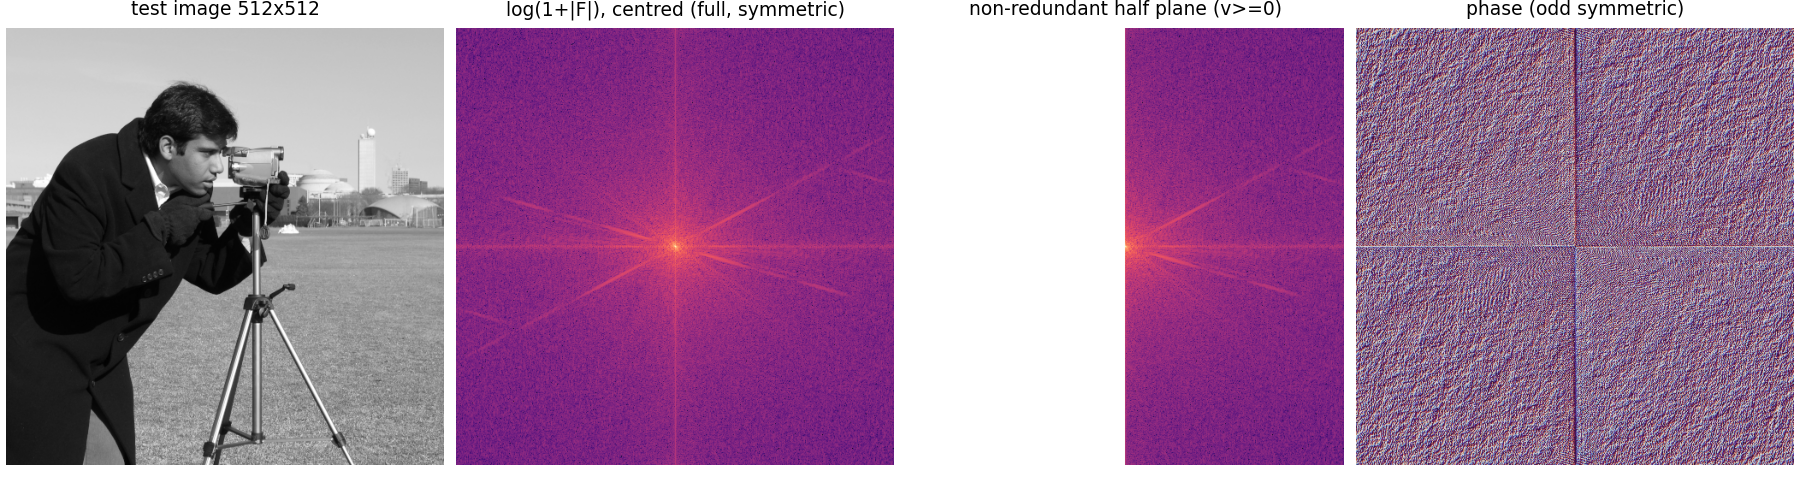
\includegraphics[width=1.00\linewidth]{q1_spectrum}\par\vskip 3pt{\small\textbf{Figure 1.1.} Test image, centred log(1+\textbar{}F\textbar{}), the non-redundant half plane (v \textgreater{}= 0) and the (odd-symmetric) phase.\par}\end{figure}
\textbf{Counting conventions (even N=512).} Under $(u,v)\mapsto(-u,-v) \bmod N$ the fixed points are exactly the four bins with $u,v\in\{0,N/2\}$. The number of conjugacy-equivalence classes (orbits) is therefore $4+(N^2-4)/2=(N^2+4)/2$, which is 131074 for N=512 (enumerated numerically: 131074). This is different from (i) the number of bins stored by \texttt{rfft2}, $N(N/2+1)=131584$, which still contains 510 redundant entries (the conjugate-symmetric pairs inside the two columns $v=0$ and $v=N/2$), and (ii) the number of independent real degrees of freedom: each of the 4 self-conjugate bins is real (1 DOF) and each of the other $(N^2-4)/2$ classes is complex (2 DOF), giving $4+(N^2-4)=N^2=262144$, equal to the number of pixels, as it must for an invertible transform. For odd N only DC is self-conjugate ($(N^2+1)/2=130561$ classes).

\begin{table}[H]\centering\small{\small\textbf{Table 1.2.} Counting of spectral quantities for N=512 (enumerated by code, tests/test\_q1.py).\par}\vskip 3pt
\resizebox{\ifdim\width>\linewidth\linewidth\else\width\fi}{!}{\begin{tabular}{lr}\toprule
\textbf{Quantity} & \textbf{Value}\\\midrule
self-conjugate bins (fixed points) & 4\\
conjugacy classes = (N\textasciicircum{}2+4)/2 & 131074\\
real degrees of freedom (= N\textasciicircum{}2) & 262144\\
bins stored by rfft2 = N(N/2+1) & 131584\\
redundant entries inside rfft2 storage & 510\\
real numbers stored by rfft2 & 263168\\
\bottomrule\end{tabular}}\end{table}
\subsection{1.1b Verification of the shift and circular-convolution theorems}
\textbf{Shift theorem.} If $g[r,c]=f[(r-a)\bmod N,(c-b)\bmod N]$ then, substituting $r'=r-a$, $c'=c-b$,

\begin{equation}G(u,v)=e^{-2\pi i (ua+vb)/N}\,F(u,v)\end{equation}
so the magnitude is unchanged and the phase changes linearly by $-2\pi(ua+vb)/N$. Table 1.3 compares $G$ computed by the custom DFT of the shifted test image with the prediction (right-hand side); phase errors are evaluated on the 5717 bins with $|F|>10^{-3}\max|F|$ (below that the phase of a numerically tiny bin is meaningless).

\begin{table}[H]\centering\footnotesize{\small\textbf{Table 1.3.} Shift theorem: measured vs theoretical prediction. Columns: max\textbar{}DFT(shifted) - F e\textasciicircum{}\{-2 pi i (ua+vb)/N\}\textbar{}; the same relative to max\textbar{}F\textbar{} = 3.38e7; max over bins of \textbar{}\textbar{}F\_s\textbar{}-\textbar{}F\textbar{}\textbar{} (theory: 0); max phase deviation from the predicted linear phase (rad); max spatial error after inverting the predicted spectrum vs np.roll (theory: 0).\par}\vskip 3pt
\resizebox{\ifdim\width>\linewidth\linewidth\else\width\fi}{!}{\begin{tabular}{lrrrrr}\toprule
\textbf{shift (a,b)} & \textbf{max abs err} & \textbf{\begin{tabular}[b]{@{}c@{}}rel. to\\{}max\textbar{}F\textbar{}\end{tabular}} & \textbf{\begin{tabular}[b]{@{}c@{}}max\\{}\textbar{}\textbar{}Fs\textbar{}-\textbar{}F\textbar{}\textbar{}\end{tabular}} & \textbf{\begin{tabular}[b]{@{}c@{}}max phase\\{}err (rad)\end{tabular}} & \textbf{spatial err}\\\midrule
(0, 0) & 0.00e+00 & 0.00e+00 & 0.00e+00 & 0.00e+00 & 6.39e-12\\
(1, 0) & 6.16e-09 & 1.82e-16 & 6.05e-09 & 3.42e-14 & 6.11e-12\\
(0, 1) & 6.77e-09 & 2.00e-16 & 4.19e-09 & 5.51e-14 & 6.59e-12\\
(5, 3) & 2.33e-08 & 6.90e-16 & 6.52e-09 & 6.71e-14 & 6.42e-12\\
(-17, 40) & 3.46e-08 & 1.02e-15 & 4.66e-09 & 7.06e-14 & 5.85e-12\\
(100, -37) & 2.55e-07 & 7.53e-15 & 4.66e-09 & 1.24e-13 & 9.09e-12\\
(256, 256) & 1.65e-06 & 4.88e-14 & 4.89e-09 & 3.52e-13 & 2.98e-11\\
(333, 101) & 1.82e-06 & 5.38e-14 & 6.52e-09 & 3.32e-13 & 3.09e-11\\
(511, 511) & 1.15e-06 & 3.41e-14 & 6.52e-09 & 6.57e-13 & 5.15e-11\\
\bottomrule\end{tabular}}\end{table}
\textbf{Circular convolution theorem.} With $(f\circledast g)[r,c]=\sum_{a,b} f[a,b]\,g[(r-a) \bmod N,(c-b) \bmod N]$,

\begin{equation}\mathrm{DFT}\{f\circledast g\}(u,v)=F(u,v)\,G(u,v)\end{equation}
The \textit{reference} convolution is computed directly in the spatial domain by summing rolled copies of the image, $\sum_{m,n}K[m,n]\,f[(r-m+c_m) \bmod N,(c-n+c_n) \bmod N]$ (no FFT involved); the \textit{tested} value is $\mathrm{IDFT}\{F\,G\}$ with the custom DFT. Errors are defined as: absolute $\max|a-b|$; relative-L2 $\|a-b\|_2/\|a\|_2$; and max error divided by $\max|a|$ ($a$ = direct spatial result).

\begin{table}[H]\centering\footnotesize{\small\textbf{Table 1.4.} Circular convolution theorem on the 512x512 test image (kernel origin at its centre, wrapped).\par}\vskip 3pt
\resizebox{\ifdim\width>\linewidth\linewidth\else\width\fi}{!}{\begin{tabular}{lrrrrr}\toprule
\textbf{kernel} & \textbf{taps} & \textbf{max\textbar{}direct\textbar{}} & \textbf{max abs err} & \textbf{\begin{tabular}[b]{@{}c@{}}max abs err\\{}/\\{}max\textbar{}direct\textbar{}\end{tabular}} & \textbf{rel. L2 err}\\\midrule
Laplacian 5x5 & 25 & 1.85e+03 & 6.53e-11 & 3.53e-14 & 1.33e-14\\
Sobel 3x3 & 9 & 8.60e+02 & 1.74e-11 & 2.03e-14 & 9.47e-15\\
Gaussian 15x15 (sigma=3) & 225 & 2.43e+02 & 1.14e-12 & 4.68e-15 & 1.35e-15\\
random positive 63x63 & 3969 & 2.18e+02 & 1.73e-12 & 7.95e-15 & 2.13e-15\\
\bottomrule\end{tabular}}\end{table}
The dual statement $\mathrm{DFT}\{f\cdot g\}=\frac{1}{N^2}F\circledast G$ was verified on a 32x32 crop windowed by a Hann function: max abs error 1.76e-10 (1.80e-15 relative). All discrepancies are at rounding level; the identities hold exactly in exact arithmetic.

\subsection{1.1c Sinusoid parameter recovery and the resolution limit}
\textbf{Synthetic image (ground truth).} $f[r,c]=\sum_{i=1}^{4} A_i\cos\!\big(2\pi(u_i r+v_i c)/N+\phi_i\big)$ with $N=512$ and the parameters listed as 'true' in Table 1.5. A real cosine with parameters $(u,v,A,\phi)$ produces two spectral lines, $F(\pm u,\pm v)=\frac{AN^2}{2}e^{\pm i\phi}$; the recovery below therefore uses only the half plane $u>0$ (or $u=0,v>0$): frequency = peak position, $A=2|F|/N^2$, $\phi=\angle F$. The peak picker (local maxima of $|F|$ above $10^{-3}\max|F|$) uses no ground-truth information.

\begin{table}[H]\centering\scriptsize{\small\textbf{Table 1.5.} True vs recovered parameters (noise-free, half-plane convention: signs of (u,v) and phi flipped where the true frequency lies in the other half plane).\par}\vskip 3pt
\resizebox{\ifdim\width>\linewidth\linewidth\else\width\fi}{!}{\begin{tabular}{lrrlrrrr}\toprule
\textbf{true (u,v)} & \textbf{true A} & \textbf{true phi} & \textbf{rec. (u,v)} & \textbf{rec. A} & \textbf{rec. phi} & \textbf{A error} & \textbf{\begin{tabular}[b]{@{}c@{}}phi error\\{}(rad)\end{tabular}}\\\midrule
(12, 20) & 100.000 & 0.5000 & (12, 20) & 100.000000 & 0.500000 & 0.00e+00 & -3.55e-15\\
(45, -30) & 60.000 & 1.2000 & (45, -30) & 60.000000 & 1.200000 & -7.11e-15 & -3.11e-15\\
(70, -15) & 40.000 & 2.0000 & (70, -15) & 40.000000 & 2.000000 & 7.11e-15 & -6.22e-15\\
(5, 5) & 25.000 & -2.5000 & (5, 5) & 25.000000 & -2.500000 & 0.00e+00 & -8.88e-16\\
\bottomrule\end{tabular}}\end{table}
With additive Gaussian noise of standard deviation 5.0 (not part of the ground truth) the same procedure returns amplitudes 100.014, 60.006, 39.999, 24.984 and phases 0.4999, 1.2002, 2.0005, -2.5000, i.e. errors below 0.02 in amplitude and 0.001 rad in phase, because the DFT averages $N^2=262144$ noisy samples per bin (error std $\approx\sigma\sqrt{2/N^2}$).

\textbf{Resolution limit.} For a sinusoid of frequency $f_0$ (cycles/pixel) observed on $N$ samples, the DFT bin spacing is $\Delta f=1/N$ cycles/pixel (1 cycle per image); the continuous spectrum of the rectangular observation window is the Dirichlet kernel

\begin{equation}W_N(f-f_0)=\sum_{n=0}^{N-1} e^{-2\pi i (f-f_0)n}=e^{-i\pi (N-1)(f-f_0)}\,\frac{\sin(\pi N (f-f_0))}{\sin(\pi (f-f_0))}\end{equation}
whose main lobe has null-to-null width $2/N$. The origin of the limit is the finite window: a signal observed over $T=N$ samples cannot resolve frequencies closer than $\sim 1/T$ (time-frequency uncertainty). Bins at integer multiples of $1/N$ see each other's kernels at nulls (orthogonality), so on-grid sinusoids are recovered exactly (Table 1.5); off-grid sinusoids leak. Test: a component at $u=40.5$ (half a bin) gives a grid peak of $A_\mathrm{peak}=50.930$ instead of 80, i.e. a ratio 0.6366, which equals the predicted scalloping loss $|\mathrm{sinc}(0.5)|=2/\pi=0.6366$ for one axis half a bin off-grid; zero padding by 4 recovers $(u,v)=(40.5,22)$ and $A=80.000$.

\begin{table}[H]\centering\footnotesize{\small\textbf{Table 1.6.} Two equal-amplitude sinusoids at u = 50 and u = 50 + delta (v = 0) on N = 512 samples; the spectrum is evaluated with 16x zero padding and the number of main lobes (\textgreater{}= 50\% of the maximum) and the valley depth between them are reported. 'Resolved' means two main lobes with valley \textless{} 0.9 of the lower peak.\par}\vskip 3pt
\resizebox{\ifdim\width>\linewidth\linewidth\else\width\fi}{!}{\begin{tabular}{lrrlrr}\toprule
\textbf{delta (bins)} & \textbf{\begin{tabular}[b]{@{}c@{}}relative\\{}phase\end{tabular}} & \textbf{main peaks} & \textbf{\begin{tabular}[b]{@{}c@{}}peak\\{}locations\end{tabular}} & \textbf{\begin{tabular}[b]{@{}c@{}}valley/lower\\{}peak\end{tabular}} & \textbf{resolved}\\\midrule
0.5 & in phase & 1 & 50.25 & n/a & no\\
0.5 & quadrature & 2 & 49.56, 50.94 & 0.00429 & yes\\
0.75 & in phase & 2 & 49.75, 51.00 & 0.677 & yes\\
0.75 & quadrature & 2 & 49.75, 51.00 & 0.667 & yes\\
1.0 & in phase & 2 & 49.81, 51.19 & 0.00876 & yes\\
1.0 & quadrature & 2 & 50.00, 51.00 & 0.901 & no\\
1.25 & in phase & 2 & 49.94, 51.31 & 0.311 & yes\\
1.25 & quadrature & 2 & 50.19, 51.06 & 0.965 & no\\
1.5 & in phase & 2 & 50.00, 51.50 & 0.41 & yes\\
1.5 & quadrature & 2 & 49.94, 51.56 & 0.764 & yes\\
2.0 & in phase & 2 & 49.88, 52.12 & 1.8e-15 & yes\\
2.0 & quadrature & 2 & 50.00, 52.00 & 2.5e-15 & yes\\
3.0 & in phase & 2 & 49.94, 53.12 & 9.0e-16 & yes\\
3.0 & quadrature & 2 & 50.00, 53.00 & 1.5e-15 & yes\\
\bottomrule\end{tabular}}\end{table}
Reading the table: separations below one bin merge into one lobe or give biased peak positions; between about 0.75 and 1.5 bins the outcome depends on the relative phase of the two components (interference of the two Dirichlet kernels shifts and distorts the lobes), and from 2 bins (the null-to-null width) the components are always separated with a valley at the numerical zero. Hence the \textit{guaranteed}, phase-independent resolution is $2\Delta f=2/N$ and the \textit{nominal} grid resolution is $\Delta f=1/N$ cycles/pixel (here 0.00195 cycles/pixel = 1 cycle/image).

\begin{figure}[H]\centering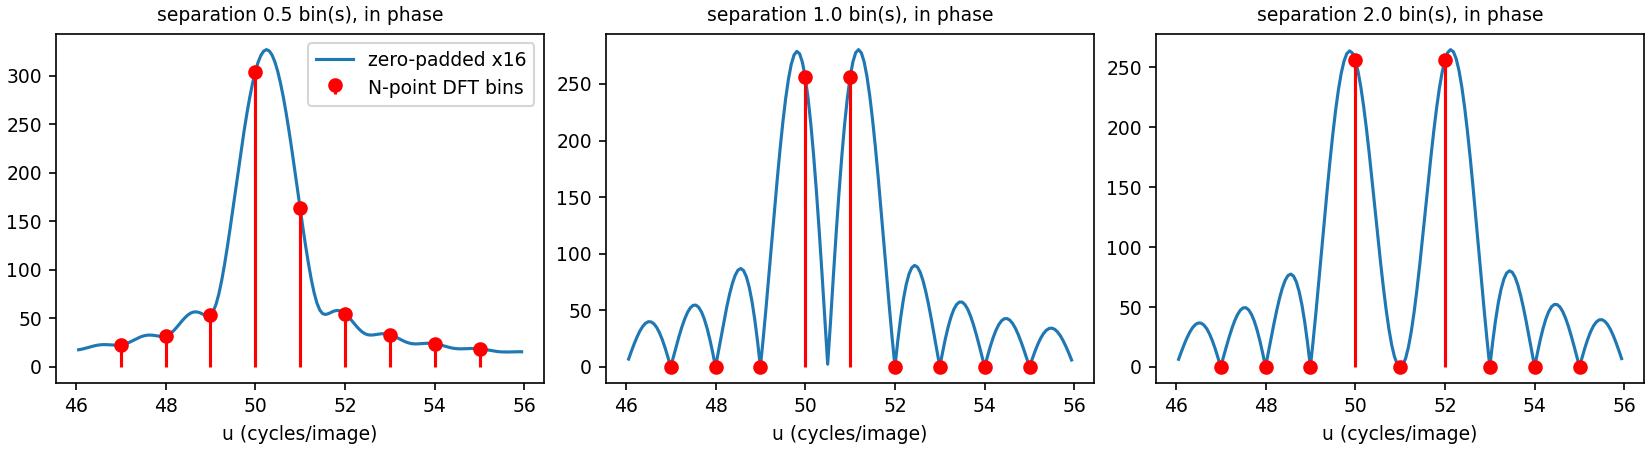
\includegraphics[width=1.00\linewidth]{q1_resolution}\par\vskip 3pt{\small\textbf{Figure 1.2.} Resolution experiment: zero-padded spectrum (blue) and the N-point DFT bins (red) for separations of 0.5, 1 and 2 bins.\par}\end{figure}
\begin{figure}[H]\centering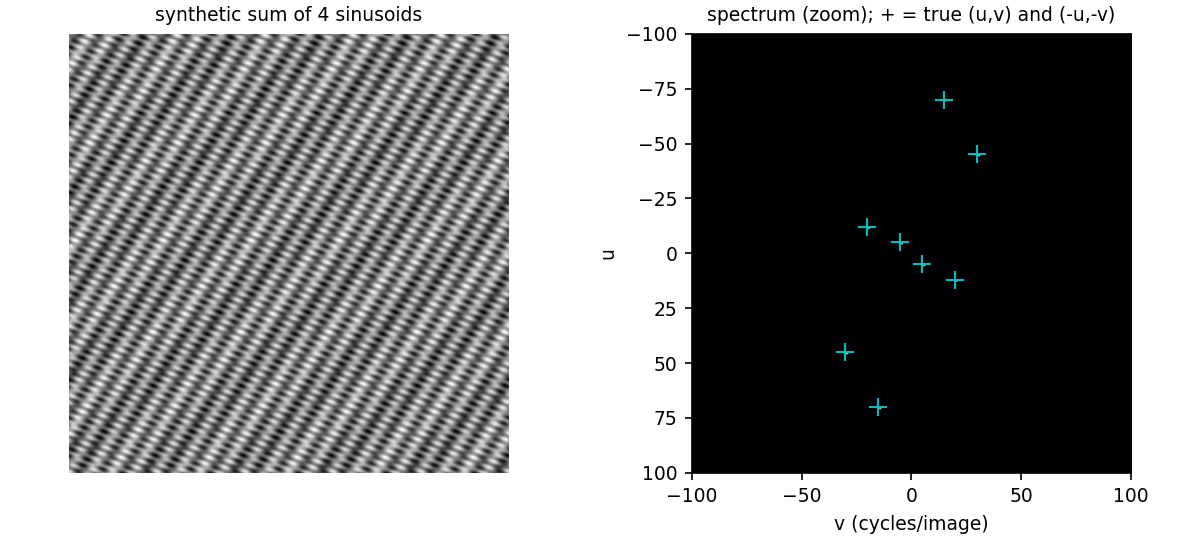
\includegraphics[width=0.85\linewidth]{q1_sinusoid}\par\vskip 3pt{\small\textbf{Figure 1.3.} Synthetic four-sinusoid image and the zoomed spectrum with the true (u,v) and (-u,-v) positions overlaid.\par}\end{figure}
\subsection{1.2 Phase versus magnitude}
\textbf{Pre-implementation prediction} (full text in \texttt{predictions/\allowbreak{}q1\_\allowbreak{}2\_\allowbreak{}prediction.\allowbreak{}md}, written 2026-10-27 11:17:12 +0530, sha256 58f5812245c8794a...; the experiment was run at 2026-10-27 11:55:26).

\begin{itemize}\item Flat magnitude $c$: $\hat f=c\,\mathrm{IDFT}[F/|F|]=c\,(f\circledast w)$ with the zero-phase whitening kernel $w=\mathrm{IDFT}[1/|F|]$. By the shift theorem an impulse keeps its position (its phase carries the position); phase is not additive, so superposition fails and the result is the image filtered by $1/|F|\sim|k|^{\alpha}$, a strong high-pass: contours and texture at their original positions, low-frequency tone lost, sparse heavy-tailed edge-map-like appearance. \item Exact consequences: $\hat f$ real; $\sum\hat f^2=c^2$ (Parseval); mean $=c/N^2$; flat radial power spectrum. \item Heuristics (not exact): smoothed $|\hat f|$ correlates with the gradient magnitude (predicted $r>0.3$); correlation of $\hat f$ with $f$ small (predicted $|r|<0.1$). \item White-noise magnitude $R$ (Rayleigh-like, independent of the phase): $\mathrm{corr}(\hat f_R,\hat f_{flat})=E[R]/\sqrt{E[R^2]}=\sqrt\pi/2=0.886$. \item Zero phase: $\hat f=\mathrm{IDFT}|F|$ is real and even, maximum at the origin equal to $\sum|F|/N^2$, no localisation: a smooth centred blob. \end{itemize}
\begin{figure}[H]\centering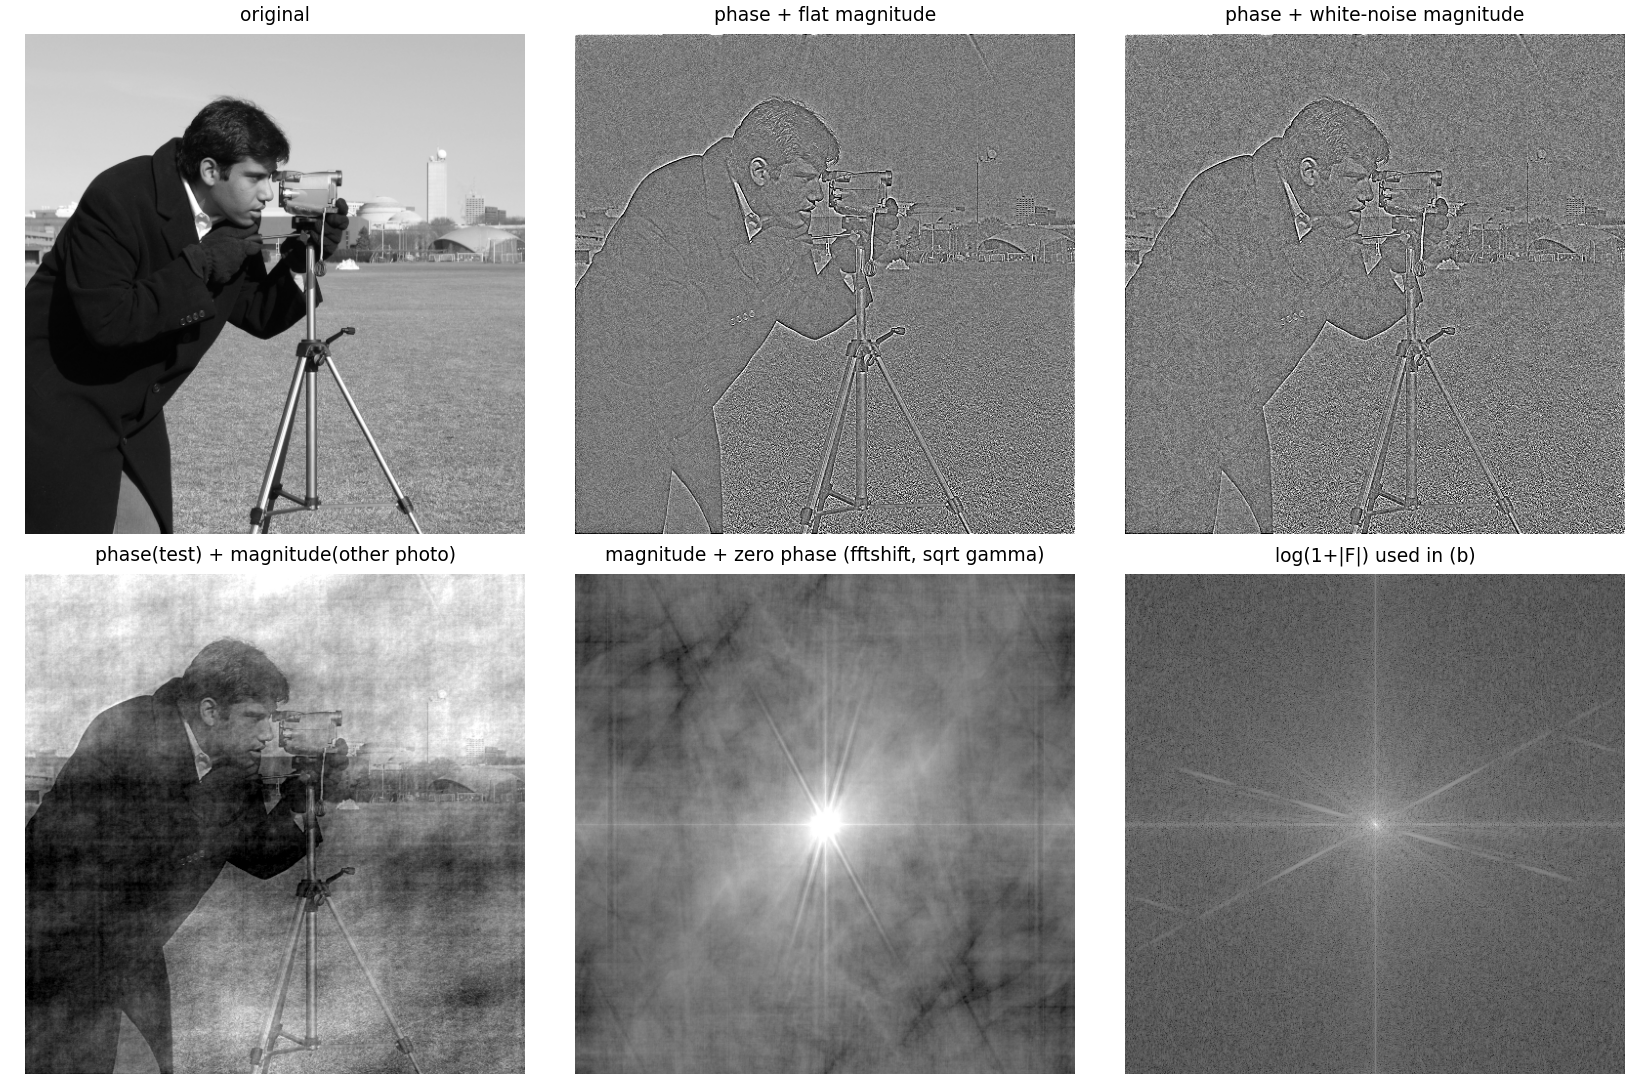
\includegraphics[width=1.00\linewidth]{q1_phase_magnitude}\par\vskip 3pt{\small\textbf{Figure 1.4.} Phase-only reconstructions and the zero-phase reconstruction. Top: original; phase + flat magnitude; phase + white-noise magnitude. Bottom: phase of the test image + magnitude of a different photograph; magnitude + zero phase (fftshifted, square-root display); the log-magnitude spectrum used in (b).\par}\end{figure}
\begin{table}[H]\centering\small{\small\textbf{Table 1.7.} Pre-implementation predictions vs measurements (Section 1.2).\par}\vskip 3pt
\resizebox{\ifdim\width>\linewidth\linewidth\else\width\fi}{!}{\begin{tabular}{p{5.2cm}p{3.5cm}p{3.2cm}p{3.5cm}}\toprule
\textbf{quantity} & \textbf{prediction} & \textbf{measured} & \textbf{status}\\\midrule
f\_hat (flat) is real: max\textbar{}Im\textbar{}/max\textbar{}Re\textbar{} & 0 (exact) & 1.16e-15 & confirmed (rounding)\\
Parseval: sum f\_hat\textasciicircum{}2 / c\textasciicircum{}2 & 1 & 1 & confirmed\\
mean(f\_hat) N\textasciicircum{}2 / c & 1 & 1 & confirmed\\
flatness of radial power std/mean & 0 & 4.71e-16 & confirmed\\
corr(f\_hat, f) & \textbar{}r\textbar{} \textless{} 0.1 (heuristic) & 0.1841 & NOT confirmed; see text\\
corr(smoothed \textbar{}f\_hat\textbar{}, smoothed \textbar{}grad f\textbar{}) & \textgreater{} 0.3 & 0.859 & confirmed\\
kurtosis of f\_hat (Gaussian = 3; f: 1.69) & heavy-tailed (\textgreater{} 3) & 8.07 & confirmed\\
corr(f\_hat\_noise-magnitude, f\_hat\_flat) & 0.886 +- 0.01 & 0.8860 & confirmed\\
zero phase: f\_hat real / even (rel. err) & 0 / 0 & 2.09e-16 / 1.61e-16 & confirmed\\
zero phase: argmax and max value & (0,0), sum\textbar{}F\textbar{}/N\textasciicircum{}2 = 7071.55 & (0, 0), 7071.55 & confirmed\\
\bottomrule\end{tabular}}\end{table}
\textbf{Reconciliation.} All exact predictions are confirmed to rounding precision, and the qualitative description (outlines and texture at the right places, no tone, heavy tails; Figure 1.4, top middle) is correct. One heuristic bound was wrong: the correlation of $\hat f$ with $f$ was predicted to be below 0.1 in magnitude but measured 0.184. The error was in the heuristic, not in the theory: by Parseval the correlation between $f-\bar f$ and $\hat f=\mathrm{IDFT}[F/|F|]$ is exactly $\sum_{k\ne0}|F_k|/\sqrt{K\sum_{k\ne 0}|F_k|^2}=E|F|/\sqrt{E|F|^2}$ over the non-DC bins, because $F\,\overline{F/|F|}=|F|$ is positive in every bin. For this image that ratio is 0.1841 (the measured value is 0.1841): positive and small, because the spread of $|F|$ over six decades makes $E|F|\ll\sqrt{E|F|^2}$. The white-noise-magnitude variant agrees with $\sqrt\pi/2$ to four digits (the empirical $E[R]/\sqrt{E[R^2]}$ of the particular noise draw is 0.8860).

\textbf{Why a flat magnitude isolates structure more cleanly than a magnitude swap.} With a flat magnitude, $\hat f=c(f\circledast w)$ contains \textit{only} information of $f$ (its measured correlation with the second photograph is 0.008, i.e. none). With another natural image's magnitude, $\hat f=f\circledast\mathrm{IDFT}[|G|/|F|]$: since $|G|$ has the typical $1/k^\alpha$ envelope, the result keeps most of the low-frequency energy and mixes in the donor's amplitude structure: its correlation with $f$ is 0.877 (tone and layout of $f$ visible, Figure 1.4 bottom left) but it is also correlated with the donor image (0.402) and its gradient-magnitude correlation drops to -0.117. The swap therefore reflects the \textit{product} of two sets of statistics, while the flat magnitude removes every amplitude cue so that what remains is attributable to phase (position) alone.

\textbf{(b) Zero phase.} With $\angle F\equiv 0$, $\hat f=\mathrm{IDFT}|F|$. Because $|F|$ is real, non-negative and even, $\hat f$ is real and even ($\hat f(x,y)=\hat f(-x,-y)$; measured asymmetry 1.61e-16) and all spectral components add constructively at the origin, so the global maximum sits at $(0,0)$ and equals $\sum|F|/N^2=7071.55$ (measured 7071.55). No linear phase means no position information: structure is not localised; the image is a centrally symmetric blob whose radial profile is the square-root of the power spectrum (a smooth, sharply peaked core with streaks from the dominant edge orientations). 10.4\% of its energy lies within 16 px of the origin (the test image: 0.34\%).

\subsection{1.3 Padding, wraparound and computational overhead}
A $5\times5$ Laplacian-of-Gaussian-type kernel $K$ and the $3\times3$ Sobel kernel are applied to the 512x512 test image by multiplying DFTs. The \textit{linear} reference is computed by direct spatial summation with zeros outside the image (no FFT). Figure 1.5 compares the unpadded circular result with the zero-padded linear result.

\begin{figure}[H]\centering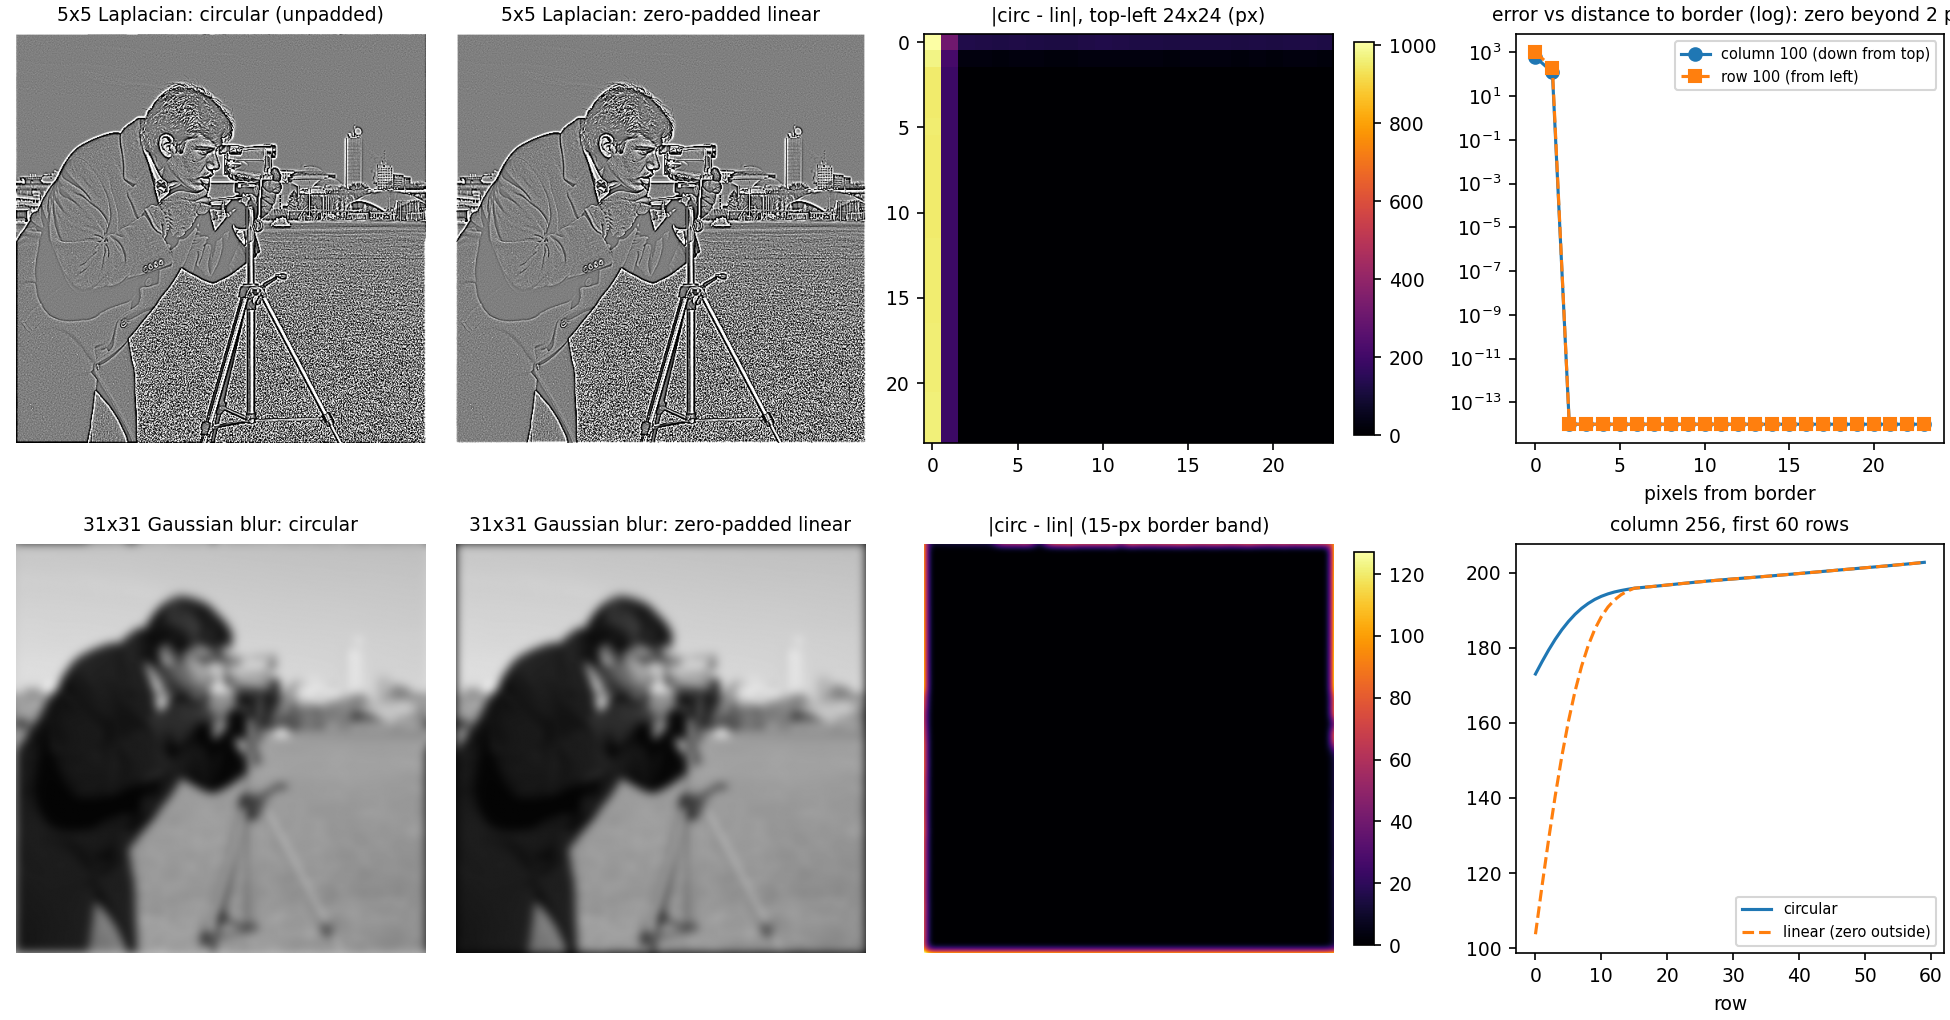
\includegraphics[width=1.00\linewidth]{q1_wraparound}\par\vskip 3pt{\small\textbf{Figure 1.5.} Wraparound evidence. Top row: 5x5 Laplacian, circular vs linear and the error confined to the first 2 pixels from the border (log plot: exactly zero beyond). Bottom row: a 31x31 Gaussian low-pass makes the border difference plainly visible: the circular result mixes in content from the opposite edge of the image (bright sky at the top with the ground at the bottom, dark coat at the left with the right edge), whereas the zero-padded linear result fades towards black at the border; the two differ by up to 49.9\% of full scale within the 15-pixel band (right plot: column 256, first 60 rows).\par}\end{figure}
\begin{table}[H]\centering\footnotesize{\small\textbf{Table 1.8.} Where circular and linear convolution differ: error is zero (to rounding) in the interior and non-zero only in the border band of width (M-1)/2. (Sobel: some border pixels are zero by coincidence on flat areas, so the corrupted fraction is slightly below the band area.)\par}\vskip 3pt
\resizebox{\ifdim\width>\linewidth\linewidth\else\width\fi}{!}{\begin{tabular}{lrrrrr}\toprule
\textbf{kernel} & \textbf{\begin{tabular}[b]{@{}c@{}}band width\\{}(M-1)/2\end{tabular}} & \textbf{\begin{tabular}[b]{@{}c@{}}max err\\{}interior\end{tabular}} & \textbf{\begin{tabular}[b]{@{}c@{}}max err in\\{}band\end{tabular}} & \textbf{\begin{tabular}[b]{@{}c@{}}fraction of\\{}pixels\\{}corrupted\end{tabular}} & \textbf{\begin{tabular}[b]{@{}c@{}}band area\\{}fraction\\{}1-((N-2h)/N)\textasciicircum{}2\end{tabular}}\\\midrule
Laplacian 5x5 & 2 & 0.00e+00 & 1608 & 0.01556 & 0.01556\\
Sobel 3x3 & 1 & 0.00e+00 & 948 & 0.006664 & 0.007797\\
Gaussian 31x31 (sigma=6) low-pass & 15 & 0.00e+00 & 127.29 & 0.1138 & 0.1138\\
\bottomrule\end{tabular}}\end{table}
\textbf{Minimal padding.} The linear convolution of an $N\times N$ image with an $M\times M$ kernel has support $(N+M-1)\times(N+M-1)$. The DFT product corresponds to circular convolution of period $P$; a sample at linear index $n\ge P$ lands on $n-P$ (time-domain aliasing). Exact equivalence with the linear convolution for all outputs therefore requires

\begin{equation}N_{x,\mathrm{pad}}=N_{y,\mathrm{pad}}\ \ge\ N+M-1 ,\qquad \text{minimal: } P=N+M-1=516\ \ (N=512,\,M=5)\end{equation}
Both image and kernel are zero-padded (kernel origin at index 0) to $P\times P$. The sweep of Table 1.9 confirms it: for $P<N+M-1$ the output differs from the true linear result by up to 1819 (the aliased rows), while the aliasing-folded prediction of the full linear result matches the FFT output to $10^{-11}$; at $P=516$ and above the error is $10^{-12}$. (If only the centred 'same' crop is required, aliased samples fall outside the crop when $P\ge N+(M-1)/2=514$; this is visible in the last column.)

\begin{table}[H]\centering\footnotesize{\small\textbf{Table 1.9.} Zero-padding size sweep for the 5x5 Laplacian (N=512, M=5): max error of the FFT result vs the direct linear convolution (column 4; for P \textless{} N+M-1 over the P x P block), vs the folded (aliased) linear result (column 5; theory says 0), and for the centred 'same' crop.\par}\vskip 3pt
\resizebox{\ifdim\width>\linewidth\linewidth\else\width\fi}{!}{\begin{tabular}{rrrrrr}\toprule
\textbf{P} & \textbf{P \textgreater{}= N+M-1} & \textbf{\begin{tabular}[b]{@{}c@{}}memory\\{}factor\\{}(P/N)\textasciicircum{}2\end{tabular}} & \textbf{\begin{tabular}[b]{@{}c@{}}max err vs\\{}linear\end{tabular}} & \textbf{\begin{tabular}[b]{@{}c@{}}max err vs\\{}folded\\{}linear\end{tabular}} & \textbf{\begin{tabular}[b]{@{}c@{}}max err of\\{}'same' crop\end{tabular}}\\\midrule
512 & no & 1.0000 & 1.82e+03 & 9.66e-13 & 1.61e+03\\
513 & no & 1.0039 & 1.82e+03 & 2.27e-12 & 3.49e+02\\
514 & no & 1.0078 & 1.22e+03 & 4.97e-12 & 4.97e-12\\
515 & no & 1.0118 & 2.54e+02 & 1.05e-11 & 1.05e-11\\
516 & yes & 1.0157 & 5.90e-12 & - & 5.90e-12\\
540 & yes & 1.1124 & 1.71e-12 & - & 1.71e-12\\
1024 & yes & 4.0000 & 1.37e-12 & - & 1.37e-12\\
\bottomrule\end{tabular}}\end{table}
\begin{figure}[H]\centering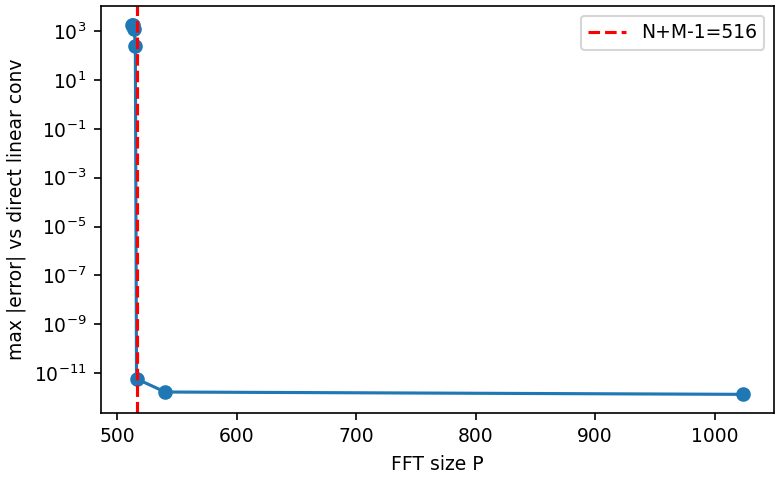
\includegraphics[width=0.50\linewidth]{q1_padding_sweep}\par\vskip 3pt{\small\textbf{Figure 1.6.} Maximum error of the padded-FFT convolution versus P: it collapses to rounding level exactly at P = N+M-1 = 516.\par}\end{figure}
\textbf{Cost of padding.} Storage grows by $(P/N)^2$ (complex arrays): 1.016 for $P=516$ and 4 for the $P=2N$ pipeline of Problem 2. A 2-D FFT of $P\times P$ points costs $\sim 5P^2\log_2(P^2)$ flops, so relative to the unpadded $N\times N$ transform the asymptotic increase is

\begin{equation}\frac{P^2\log P^2}{N^2\log N^2}=\Big(\frac{P}{N}\Big)^{2}\Big(1+\frac{\log (P/N)}{\log N}\Big),\qquad P=2N:\ 4\Big(1+\frac{1}{9}\Big)=4.44\end{equation}
i.e. still $O(N^2\log N)$ with a constant that depends on $(P/N)^2$; three transforms are needed (image, kernel, inverse). Direct spatial convolution costs $O(N^2M^2)$, so the FFT route wins beyond a kernel size of roughly $M\gtrsim 10$ on this machine (Table 1.10). \texttt{scipy.\allowbreak{}signal.\allowbreak{}fftconvolve} implements exactly this scheme: it computes the full linear shape $N+M-1$ and then pads further to \texttt{scipy.\allowbreak{}fft.\allowbreak{}next\_\allowbreak{}fast\_\allowbreak{}len(\allowbreak{}N+M-1,\allowbreak{} real=\allowbreak{}True)} because FFT length matters: $514=2\cdot257$, $526=2\cdot263$ and $516=2^2\cdot3\cdot43$ contain large prime factors and are \textit{slower} than the 5-smooth length 540 (compare the 'minimal' and 'fast length' timing columns of Table 1.10). Our padded FFT with the same length reproduces \texttt{fftconvolve} to $\le 4\times10^{-10}$ (last column).

\begin{table}[H]\centering\scriptsize{\small\textbf{Table 1.10.} Padding overhead for N=512 and M x M kernels. Memory factors (P/N)\textasciicircum{}2 for the minimal and the fast FFT length, cost-model ratio, and measured median times in ms (3 runs; machine dependent - the ratios, not the absolute times, are the result): unpadded circular, padded to N+M-1, padded to next fast length, scipy.signal.fftconvolve(full), direct spatial (rolled sums), and max difference of our fast-length result vs fftconvolve.\par}\vskip 3pt
\resizebox{\ifdim\width>\linewidth\linewidth\else\width\fi}{!}{\begin{tabular}{rrrrrrrrrrrr}\toprule
\textbf{M} & \textbf{N+M-1} & \textbf{fast len} & \textbf{mem (min)} & \textbf{mem (fast)} & \textbf{cost ratio} & \textbf{t circ} & \textbf{t pad min} & \textbf{t pad fast} & \textbf{t scipy} & \textbf{t direct} & \textbf{\begin{tabular}[b]{@{}c@{}}max diff vs\\{}scipy\end{tabular}}\\\midrule
3 & 514 & 540 & 1.008 & 1.112 & 1.008 & 24.0 & 169.0 & 30.6 & 22.9 & 28 & 9.09e-13\\
5 & 516 & 540 & 1.016 & 1.112 & 1.017 & 24.4 & 48.9 & 33.1 & 22.9 & 79 & 2.73e-12\\
9 & 520 & 540 & 1.031 & 1.112 & 1.034 & 23.9 & 34.1 & 31.7 & 23.2 & 255 & 9.09e-12\\
15 & 526 & 540 & 1.055 & 1.112 & 1.060 & 25.7 & 182.1 & 33.3 & 23.0 & 707 & 2.55e-11\\
31 & 542 & 576 & 1.121 & 1.266 & 1.131 & 24.8 & 206.5 & 36.9 & 26.5 & - & 8.73e-11\\
63 & 574 & 576 & 1.257 & 1.266 & 1.280 & 24.3 & 66.0 & 35.7 & 24.6 & - & 3.49e-10\\
\bottomrule\end{tabular}}\end{table}
\section{Question 2 - Frequency-domain filtering: ideal, Butterworth, Gaussian}
\textbf{Pipeline (used throughout).} Each $M\times N$ image is placed in the top-left corner of a $P\times P$ zero array with $P=2\max(M,N)$, transformed, multiplied by a real zero-phase $H(u,v)$ defined on the centred $P\times P$ grid with $D=\sqrt{(u-P/2)^2+(v-P/2)^2}$, inverted, the real part taken and the result cropped. Radii $D_0$ are therefore in bins of the padded grid (cycles per $P$ pixels); e.g. for the 512x512 images $P=1024$, so $D_0=40$ corresponds to $0.039$ cycles/pixel. \texttt{make\_\allowbreak{}filter(\allowbreak{}kind,\allowbreak{} P,\allowbreak{} D0,\allowbreak{} n=\allowbreak{}None,\allowbreak{} highpass=\allowbreak{}False)} (src/q2\_filtering.py) builds

\begin{equation}H_{ILPF}=\{1\ (D\le D_0),\ 0\ (D>D_0)\}\qquad H_{BLPF}=\frac{1}{1+[D/D_0]^{2n}}\qquad H_{GLPF}=e^{-D^2/(2D_0^2)}\qquad H_{HP}=1-H_{LP}\end{equation}
\subsection{2.1a Cutoff semantics and the matched Gaussian}
\begin{table}[H]\centering\small{\small\textbf{Table 2.1.} Low-pass value at D = D0 = 40 (P = 1024): analytic vs measured with make\_filter. 'GLPF matched' uses D0' = D0/sqrt(2 ln 2) = 33.97 (the value at (u,v) offset (24,32), i.e. exactly D = 40 on a diagonal, is also exactly 0.5).\par}\vskip 3pt
\resizebox{\ifdim\width>\linewidth\linewidth\else\width\fi}{!}{\begin{tabular}{lrr}\toprule
\textbf{filter} & \textbf{measured H(D0)} & \textbf{analytic}\\\midrule
ILPF & 1 & 1\\
BLPF n=1 & 0.5 & 0.5\\
BLPF n=2 & 0.5 & 0.5\\
BLPF n=5 & 0.5 & 0.5\\
GLPF (D0'=D0) & 0.606531 & 0.606531\\
GLPF matched D0'=D0/sqrt(2 ln 2) & 0.5 & 0.5\\
\bottomrule\end{tabular}}\end{table}
At $D=D_0$ the ILPF equals 1 (it jumps from 1 to 0 just beyond), the Butterworth filter equals $1/2$ for every order, and the Gaussian equals $e^{-1/2}=0.607$. The same numerical $D_0$ is therefore not like-for-like: the three filters have different attenuation at $D_0$ (ILPF has no half-amplitude point at all; the Gaussian is already above the Butterworth half-power value). Requiring $H_{GLPF}(D_0)=1/2$:

\begin{equation}e^{-D_0^2/(2D_0'^2)}=\frac12\ \Rightarrow\ D_0'=\frac{D_0}{\sqrt{2\ln 2}}=0.8493\,D_0\end{equation}
\textbf{This matched pairing is used in every later comparison}: ILPF and BLPF with $D_0$, GLPF with $D_0'=D_0/\sqrt{2\ln2}$ (Sections 2.2c, 2.3, and Problem 5). Its spatial standard deviation is derived in 2.2d. Radial profiles of the six transfer functions are in Figure 2.1.

\begin{figure}[H]\centering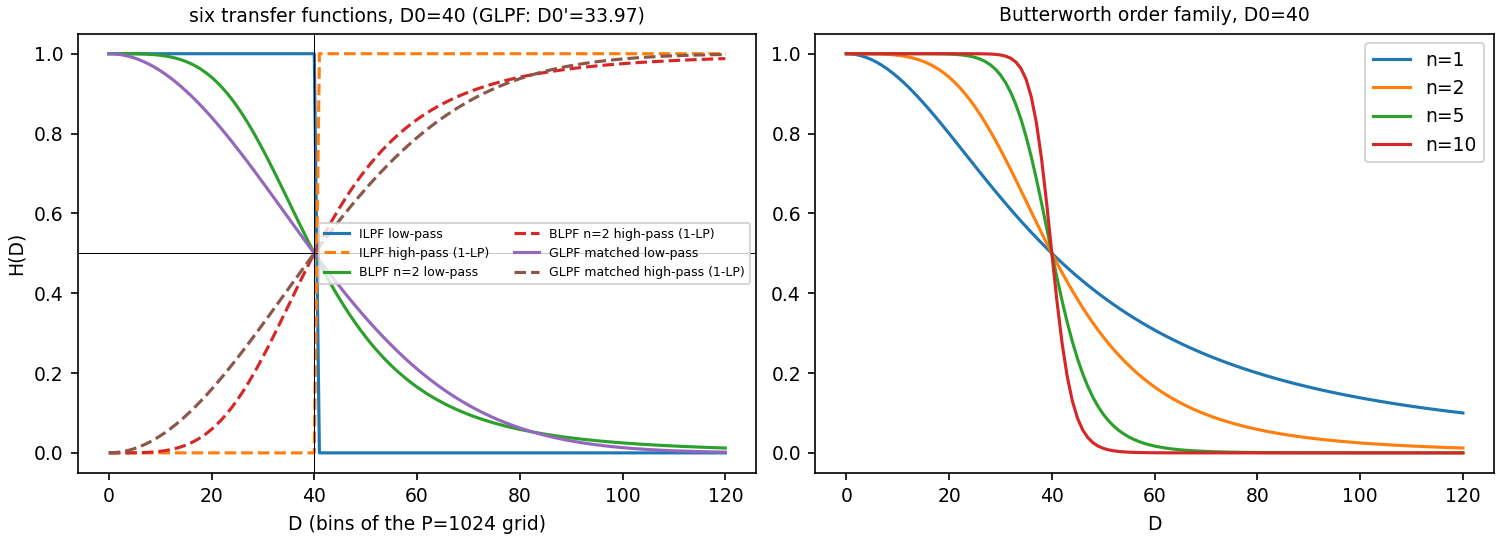
\includegraphics[width=1.00\linewidth]{q2_radial_profiles}\par\vskip 3pt{\small\textbf{Figure 2.1.} Radial profiles H(D) of the six transfer functions on a common axis (D0 = 40; GLPF with matched D0' = 33.97), and the Butterworth order family.\par}\end{figure}
\subsection{2.1b Energy-based cutoff selection}
\begin{table}[H]\centering\footnotesize{\small\textbf{Table 2.2.} Radii enclosing $\alpha(r)=100\sum_{D\le r}|F|^2/\sum|F|^2$ of the spectral power of characters\_test\_pattern.tif (688x688, zero-padded to P = 1376). Columns: smallest integer radius with alpha \textgreater{}= target (padded bins), the achieved alpha, the radius in cycles/pixel, the equivalent radius on the unpadded 688 grid, and (for comparison) the radius if the mean is removed first.\par}\vskip 3pt
\resizebox{\ifdim\width>\linewidth\linewidth\else\width\fi}{!}{\begin{tabular}{rrrrrr}\toprule
\textbf{target alpha} & \textbf{\begin{tabular}[b]{@{}c@{}}radius r\\{}(padded\\{}bins)\end{tabular}} & \textbf{\begin{tabular}[b]{@{}c@{}}achieved\\{}alpha (\%)\end{tabular}} & \textbf{\begin{tabular}[b]{@{}c@{}}r\\{}(cycles/pixel)\end{tabular}} & \textbf{\begin{tabular}[b]{@{}c@{}}r on\\{}unpadded\\{}grid\end{tabular}} & \textbf{\begin{tabular}[b]{@{}c@{}}r with DC\\{}removed\end{tabular}}\\\midrule
90 \% & 16 & 90.079 & 0.0116 & 8.0 & 378\\
95 \% & 46 & 95.013 & 0.0334 & 23.0 & 541\\
99 \% & 410 & 99.003 & 0.2980 & 205.0 & 711\\
99.5 \% & 559 & 99.501 & 0.4062 & 279.5 & 765\\
\bottomrule\end{tabular}}\end{table}
The single DC sample of the zero-padded 1376 x 1376 spectral grid carries 22.3946\% of the total spectral power. This fraction is specific to the padded grid used in this table and changes with the zero-padding resolution: with the unnormalised DFT convention used here, the DC coefficient $F(0,0)=\sum f$ is unchanged by zero-padding, whereas Parseval's relation makes the total squared-magnitude sum $\sum|F|^2=P^2\sum f^2$ scale with $P^2$. The padded DC fraction is therefore $(\sum f)^2/(P^2\sum f^2)$, which equals $(N/P)^2$ times the fraction $(\sum f)^2/(N^2\sum f^2)$ of the original unpadded 688 x 688 DFT. For the unpadded DFT the DC sample carries $\overline{f}^{2}/\overline{f^2}=89.5783\%$ of the power, and $89.5783\%\times(688/1376)^2=22.3946\%$. The mean grey level is 207 of 255 (a bright page with dark glyphs). Natural and graphic images have power spectra falling like $1/D^{\beta}$, so 90\% of the power lies within $r=16$ bins (0.012 cycles/pixel) although the Nyquist radius is 688. But power is not visual importance: the energy is dominated by the large, smooth bright background; the \textit{information} that makes the characters legible (edge positions, stroke widths, serif detail, the noise-like texture patches) is carried by the small residual power at high frequencies. A filter that keeps 99\% of the energy ($r=410$) is visually near-lossless, whereas one that keeps 95\% ($r=46$) already shows strong ringing and blur (Figure 2.4). Edges are discontinuities whose Fourier amplitude decays only as $1/D$, so many weak coefficients are needed to place them.

\subsection{2.1c Inverse design problem}
For the Butterworth low-pass $H=1/(1+(D/D_0)^{2n})$ we have $1/H-1=(D/D_0)^{2n}$. From $H(10)=16/17$: $(10/D_0)^{2n}=1/16$. From $H(40)=1/17$: $(40/D_0)^{2n}=16$. Dividing the second by the first eliminates $D_0$:

\begin{equation}\Big(\frac{40}{10}\Big)^{2n}=256\ \Rightarrow\ 4^{2n}=4^{4}\ \Rightarrow\ n=2,\qquad (10/D_0)^{4}=\frac1{16}\Rightarrow D_0=20\end{equation}
Smallest integer order with $H(2D_0)\le 1\%$: $H(2D_0)=1/(1+2^{2n})=1/(1+4^n)\le 0.01\iff 4^n\ge 99\iff n\ge 3.31$, so $n=4$ ($n=3$ gives $1/65=1.54\%$, $n=4$ gives $1/257=0.389\%$). Verification with \texttt{make\_\allowbreak{}filter} (P=1024, $D_0=20$, $n=2$): $H(10)=0.94117647$ (target $16/17=0.94117647$), $H(40)=0.058823529$ (target $1/17=0.058823529$); $H(2D_0)$ for $n=1..6$ is 0.2, 0.05882, 0.01538, 0.003891, 0.0009756, 0.0002441, so the smallest order meeting the 1\% requirement is $n=4$.

\subsection{2.2 Ringing: prediction, measurement and reconciliation}
\textbf{Pre-implementation prediction} (\texttt{predictions/\allowbreak{}q2\_\allowbreak{}2\_\allowbreak{}prediction.\allowbreak{}md}, written 2026-10-27 11:17:29 +0530, sha256 e25d2dffaab97006...; experiment run 2026-10-27 11:32:30).

Far from the corners the step image varies only along $x$; its spectrum is confined to $v=0$, so only the slice $H(u,0)$ matters: for the ILPF a 1-D ideal low-pass with cutoff $f_c=D_0/P$. Its impulse response is $2f_c\,\mathrm{sinc}(2f_cx)$ and its unit-step response is

\begin{equation}F(t)=\frac12+\frac{1}{\pi}\mathrm{Si}(2\pi f_c t),\qquad \mathrm{Si}(z)=\int_0^z\frac{\sin w}{w}\,dw\end{equation}
so $g(x)=A+(B-A)F(x-x_e)$ near one edge (and $A+(B-A)[F(x-x_1)-F(x-x_2)]$ for the square). $F'(t)=\sin(2\pi f_ct)/(\pi t)$ first vanishes at $2\pi f_c t^*=\pi$:

\begin{equation}t^{*}=\frac{1}{2f_c}=\frac{P}{2D_0},\qquad \mathrm{OS}=100\Big[\frac12+\frac{\mathrm{Si}(\pi)}{\pi}-1\Big]=100\,[0.0895]=8.95\%\ \ \text{(independent of }D_0)\end{equation}
Predicted first-peak distances for $P=1024$: 51.2, 25.6, 12.8, 6.4 px for $D_0=10,20,40,80$ (discrete-grid refinement $P/(2D_0+1)$: 48.8, 25.0, 12.6, 6.4). The Gaussian filter has the non-negative Gaussian kernel of $\sigma_s=P/(2\pi D_0')$ and its step response is a Gaussian CDF: predicted overshoot exactly 0\%.

\begin{table}[H]\centering\scriptsize{\small\textbf{Table 2.3.} ILPF on the 512x512 step image (A=50, B=200, square side 256), profile along the middle row y=256. OS = 100 (max g - B)/(B - A). 'Single-edge' = 8.95\% (prediction); 'two-edge Si' = closed form with both edges and f\_c=(D0+1/2)/P; 'measured' = assignment pipeline (zero padding, P=1024); 'x-only strip' = control experiment with an image that really depends on x only (rows identical, background padding). Peak distance from the edge at x=127.5 to the first local maximum inside the square.\par}\vskip 3pt
\resizebox{\ifdim\width>\linewidth\linewidth\else\width\fi}{!}{\begin{tabular}{rrrrrrrrr}\toprule
\textbf{D0} & \textbf{\begin{tabular}[b]{@{}c@{}}pred OS \%\\{}(single\\{}edge)\end{tabular}} & \textbf{\begin{tabular}[b]{@{}c@{}}pred OS \%\\{}(two-edge\\{}Si)\end{tabular}} & \textbf{\begin{tabular}[b]{@{}c@{}}measured OS\\{}\% (pipeline)\end{tabular}} & \textbf{\begin{tabular}[b]{@{}c@{}}measured OS\\{}\% (x-only\\{}strip)\end{tabular}} & \textbf{\begin{tabular}[b]{@{}c@{}}pred dist\\{}(P/2D0)\end{tabular}} & \textbf{\begin{tabular}[b]{@{}c@{}}pred dist\\{}(P/(2D0+1))\end{tabular}} & \textbf{\begin{tabular}[b]{@{}c@{}}measured\\{}dist (px)\end{tabular}} & \textbf{\begin{tabular}[b]{@{}c@{}}strip dist\\{}(px)\end{tabular}}\\\midrule
10 & 8.95 & 7.31 & 3.44 & 8.74 & 51.2 & 48.8 & 50.5 & 53.5\\
20 & 8.95 & 9.78 & 11.45 & 8.84 & 25.6 & 25.0 & 26.5 & 25.5\\
40 & 8.95 & 9.31 & 8.27 & 8.97 & 12.8 & 12.6 & 12.5 & 12.5\\
80 & 8.95 & 9.12 & 8.78 & 9.02 & 6.4 & 6.4 & 6.5 & 6.5\\
\bottomrule\end{tabular}}\end{table}
\begin{figure}[H]\centering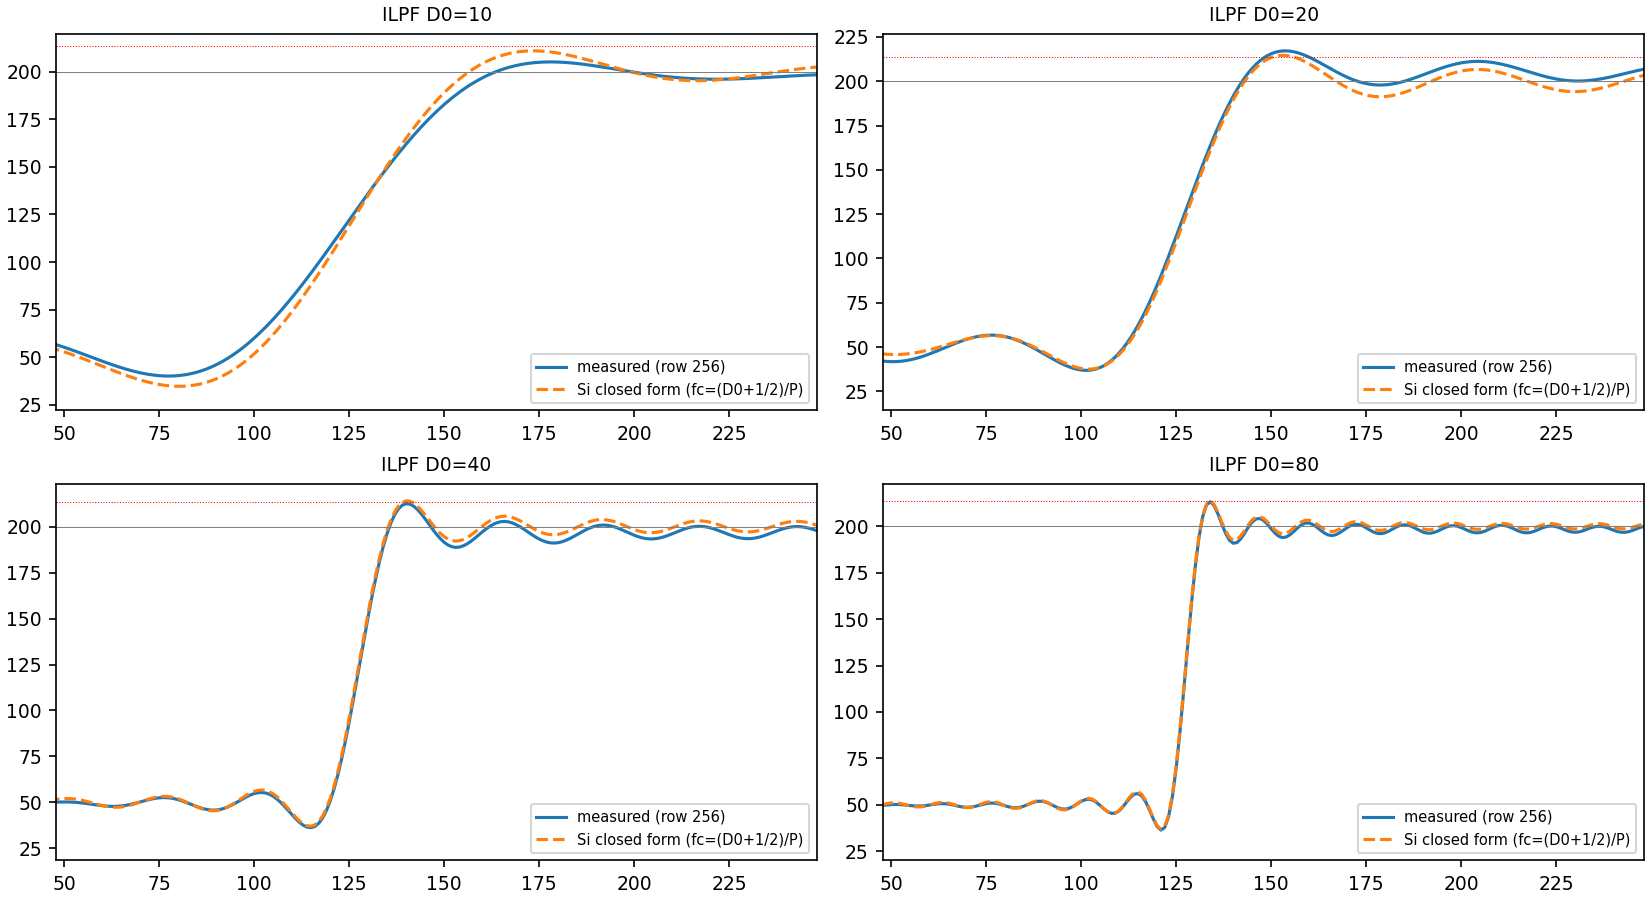
\includegraphics[width=1.00\linewidth]{q2_ringing_profiles}\par\vskip 3pt{\small\textbf{Figure 2.2.} Measured middle-row profiles (blue) vs the two-edge sine-integral closed form (dashed) for D0 = 10, 20, 40, 80; the dotted red line is the single-edge prediction B + 0.0895(B-A).\par}\end{figure}
\textbf{Reconciliation.} (i) The first-peak distances agree with the prediction to within one pixel at all four cutoffs (50.5, 26.5, 12.5, 6.5 px measured; deviations from $P/(2D_0)$: -0.7, +0.9, -0.3, +0.1 px; the discrete-grid refinement $P/(2D_0+1)$ is closer only at $D_0=40$ and not systematically better). (ii) For $D_0=40$ and $80$ the measured overshoot (8.27\%, 8.78\%) is within 0.7 and 0.2 percentage points of the 8.95\% prediction; the remaining gap is the sampling of the peak on a 1-px grid (peak width $\sim t^*$) and the second edge. (iii) For small $D_0$ the prediction fails: 3.44\% measured at $D_0=10$ and 11.45\% at $D_0=20$. The pre-implementation prediction named the zero-padding border edge as a possible cause; control experiments \textbf{rule this out for }$D_0=10$: padding with the background value $A$ (no $50\to0$ jump) still gives only 2.26\% (and 12.53\% at $D_0=20$), whereas the x-only strip reproduces the 1-D theory (8.74\%, 8.84\%, 8.97\%, 9.02\% for $D_0=10..80$, within 0.2 pp of 8.95\%, and within 1.4, 0.9, 0.3, 0.1 pp of the two-edge Si value for $D_0=10,20,40,80$; the residual at small $D_0$ comes from discrete-grid effects the closed form ignores). The dominant cause is therefore that the square is only 256 px tall while the ripple scale of the filter ($P/D_0=102$ px at $D_0=10$) is comparable: the image is not one-dimensional on that scale and the 2-D radially symmetric kernel (a jinc, not a sinc) integrates the other edges. The 1-D argument is valid only when the extent of the object in $y$ is large compared with $t^*$ (and $x$-extent with $t^*$ for the second edge's $\mathrm{Si}$ tail, which changes the overshoot by $\pm1$-2 pp at $D_0=10,20$ as the two-edge formula shows). The overshoot itself does not shrink with $D_0$: the Gibbs phenomenon only moves closer to the edge (6.5 px at $D_0=80$).

\begin{table}[H]\centering\footnotesize{\small\textbf{Table 2.4.} Gaussian low-pass (matched D0') on the step image: spatial sigma\_s = P/(2 pi D0'), measured overshoot on the profile row (0 within 1e-12 \%), maximum of the output over the whole image minus B (\textless{}= 0 up to rounding), minimum along the row.\par}\vskip 3pt
\resizebox{\ifdim\width>\linewidth\linewidth\else\width\fi}{!}{\begin{tabular}{rrrrrr}\toprule
\textbf{D0} & \textbf{D0'} & \textbf{sigma\_s (px)} & \textbf{\begin{tabular}[b]{@{}c@{}}overshoot \%\\{}(row)\end{tabular}} & \textbf{\begin{tabular}[b]{@{}c@{}}max(g) - B\\{}(whole\\{}image)\end{tabular}} & \textbf{\begin{tabular}[b]{@{}c@{}}min g along\\{}row\end{tabular}}\\\midrule
10 & 8.49 & 19.19 & -5.1e-09 & -7.72e-09 & 25.52\\
20 & 16.99 & 9.59 & 1.9e-14 & 8.53e-14 & 26.04\\
40 & 33.97 & 4.80 & 3.8e-14 & 8.53e-14 & 27.08\\
80 & 67.95 & 2.40 & 1.9e-13 & 5.68e-13 & 29.16\\
\bottomrule\end{tabular}}\end{table}
The Gaussian overshoot is zero to $10^{-13}$ at all cutoffs, as predicted (a non-negative kernel of unit sum cannot exceed $\max s$; see the proof below).

\begin{table}[H]\centering\footnotesize{\small\textbf{Table 2.5.} Profiles along rows close to the top edge of the square (corner at x=127.5): the 1-D prediction no longer applies. 'none' = the profile never rises above B (or has no interior local maximum above B).\par}\vskip 3pt
\resizebox{\ifdim\width>\linewidth\linewidth\else\width\fi}{!}{\begin{tabular}{rrrrrr}\toprule
\textbf{D0} & \textbf{\begin{tabular}[b]{@{}c@{}}row offset\\{}below top\\{}edge (px)\end{tabular}} & \textbf{\begin{tabular}[b]{@{}c@{}}OS \%\\{}measured\end{tabular}} & \textbf{\begin{tabular}[b]{@{}c@{}}first peak\\{}dist (px)\end{tabular}} & \textbf{\begin{tabular}[b]{@{}c@{}}1-D pred OS\\{}\%\end{tabular}} & \textbf{\begin{tabular}[b]{@{}c@{}}1-D pred\\{}dist\end{tabular}}\\\midrule
20 & 2 & -35.37 & none & 8.95 & 25.6\\
20 & 6 & -19.91 & none & 8.95 & 25.6\\
20 & 16 & 8.85 & 27.5 & 8.95 & 25.6\\
20 & 64 & 8.65 & 25.5 & 8.95 & 25.6\\
20 & 128 & 11.45 & 26.5 & 8.95 & 25.6\\
40 & 2 & -25.62 & none & 8.95 & 12.8\\
40 & 6 & 1.28 & 13.5 & 8.95 & 12.8\\
40 & 16 & 16.64 & 13.5 & 8.95 & 12.8\\
40 & 64 & 11.92 & 12.5 & 8.95 & 12.8\\
40 & 128 & 8.27 & 12.5 & 8.95 & 12.8\\
\bottomrule\end{tabular}}\end{table}
\textbf{Near a corner} (rows 2-16 px from the top edge) the profile is a mixture of $x$- and $y$-ripples: the image is not a function of $x$ only, its spectrum has energy off the line $v=0$ where the radial filter cuts at $|u|<\sqrt{D_0^2-v^2}$, so the effective 1-D cutoff in $u$ is smaller and depends on $v$, and the response is the 2-D jinc convolved with a quarter-plane. The overshoot is then strongly modulated: at $D_0=40$ it is $-25.6\%$ (row 2: the profile never reaches $B$ because the blurred top edge is still rising), 1.3\% (row 6), 16.6\% (row 16: constructive superposition of the $x$-ripple and the $y$-ripple, 1.9 times the 1-D value) and returns towards 8.3\% at 128 px (middle row).

\subsection{2.2b Butterworth order sweep}
\begin{table}[H]\centering\footnotesize{\small\textbf{Table 2.6.} Butterworth low-pass at D0 = 40 (P=1024): measured overshoot on the middle row, 1-D kernel h(x) = IDFT\{H(u,0)\} extrema and the ratio \textbar{}min h\textbar{}/max h. Ideal-filter limit (prediction): 8.95\%; ILPF measured with the same pipeline: 8.27\%.\par}\vskip 3pt
\resizebox{\ifdim\width>\linewidth\linewidth\else\width\fi}{!}{\begin{tabular}{rrrrrr}\toprule
\textbf{n} & \textbf{overshoot \%} & \textbf{\begin{tabular}[b]{@{}c@{}}first peak\\{}dist (px)\end{tabular}} & \textbf{max h} & \textbf{min h} & \textbf{\begin{tabular}[b]{@{}c@{}}\textbar{}min h\textbar{}/max\\{}h\end{tabular}}\\\midrule
1 & 0.000 & none & 0.1166 & -2.94e-07 & 2.52e-06\\
2 & 3.359 & 13.5 & 0.08676 & -0.003749 & 0.04321\\
3 & 5.603 & 12.5 & 0.08181 & -0.007906 & 0.09664\\
5 & 7.499 & 12.5 & 0.07943 & -0.01253 & 0.1577\\
10 & 8.486 & 12.5 & 0.07845 & -0.01569 & 0.1999\\
20 & 8.434 & 12.5 & 0.07821 & -0.01661 & 0.2124\\
ILPF (ref.) & 8.269 & 12.5 & - & - & 0.2173\\
GLPF (ref.) & 0 & - & - & - & 6.3e-17\\
\bottomrule\end{tabular}}\end{table}
\begin{figure}[H]\centering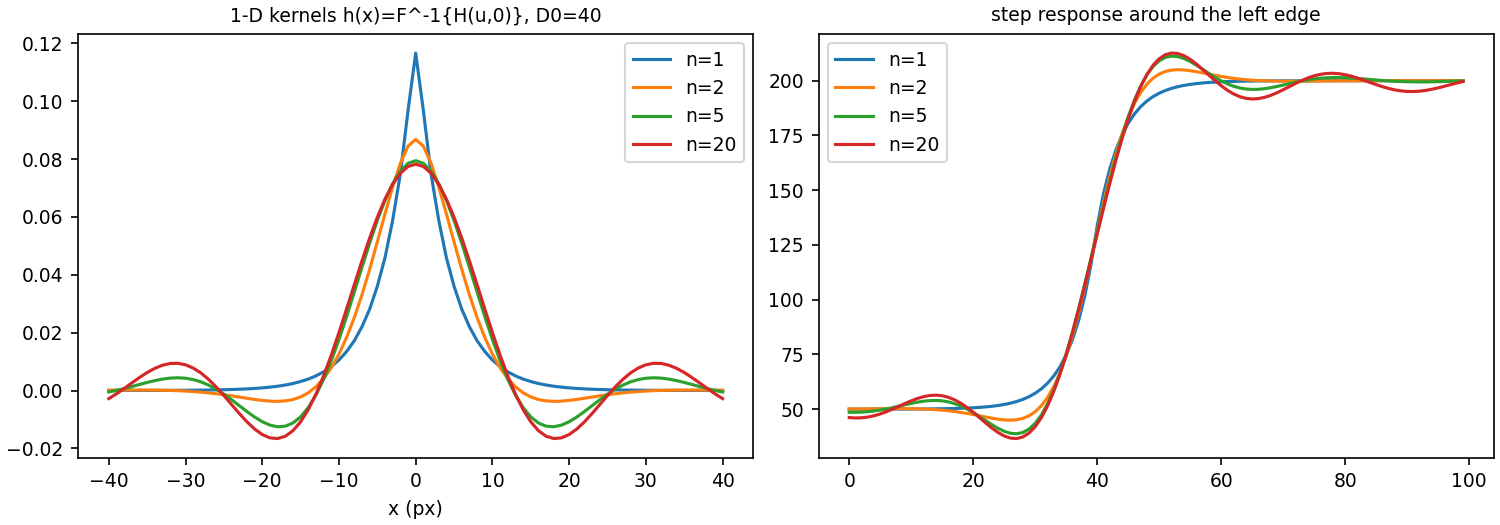
\includegraphics[width=1.00\linewidth]{q2_butterworth_kernels}\par\vskip 3pt{\small\textbf{Figure 2.3.} Left: 1-D spatial kernels h(x) = F\textasciicircum{}-1\{H(u,0)\} of the Butterworth filters at D0=40: n=1 is positive, higher orders develop negative side lobes. Right: step responses.\par}\end{figure}
\textbf{Why no ringing for n=1 but ringing for higher orders.} For $n=1$, $H(u,0)=1/(1+(u/D_0)^2)$ is a Lorentzian whose inverse transform is the two-sided exponential $\propto e^{-2\pi D_0|x|/P}$, strictly positive: $|\min h|/\max h=2.5\times10^{-6}$ (the tiny negative value is the discrete Nyquist truncation, $H(P/2)=0.006$), and the measured overshoot is $9\times10^{-6}$\%. As $n$ grows the kernel acquires negative side lobes (ratio 0.043, 0.097, 0.158, 0.200, 0.212 for $n=2,3,5,10,20$, approaching the ILPF's 0.217) and the overshoot grows monotonically with this ratio: 3.36\%, 5.60\%, 7.50\%, 8.49\%, 8.43\% towards the ideal-filter limit (8.95\% predicted, 8.27\% measured for the ILPF with the same pipeline; the last two values are within the sampling error of each other). The unit-step response is the running sum of the kernel, $s(x)=\sum_{t\le x}h(t)$, which overshoots exactly when the kernel has negative lobes.

\textbf{Proof that a non-negative, unit-sum kernel cannot overshoot.} Let $h\ge0$, $\sum h=1$ and $g=h\ast s$, i.e. $g(x)=\sum_t h(t)s(x-t)$. Because the weights are non-negative and sum to one, $g(x)$ is a convex combination of values of $s$, so $\min s\le g(x)\le\max s$ for all $x$; for the step image $A\le g\le B$, so $\mathrm{OS}\le0$. Moreover the step response $\sum_{t\le x}h(t)$ is non-decreasing because every increment $h(t)\ge0$, so it is monotone. Conversely, overshoot requires $\sum_{t\le x}h(t)>1$ for some $x$, i.e. a negative part of $h$. For the 2-D filter acting on an x-only image, the relevant 1-D kernel is the projection (marginal) of the 2-D kernel, which is again non-negative when the 2-D kernel is: the Gaussian satisfies the hypothesis (its kernel is a positive Gaussian, ratio $6\times10^{-17}$ numerically), the ideal filter and Butterworth $n\ge2$ do not.

\subsection{2.2c Visual comparison on the characters test pattern}
ILPF, BLPF ($n=2$) and GLPF (matched $D_0'=D_0/\sqrt{2\ln2}$) were applied at the four radii of Table 2.2 ($D_0=16, 46, 410, 559$, i.e. alpha = 90/95/99/99.5\%). Figure 2.4 shows the grid; red arrows R1 and R2 mark two locations where ILPF ringing is visible at $D_0=46$ (concentric ripples around the circles at R1 and the squares at R2, also the periodic 'ghost' ripples across the whole flat background), and Figure 2.5 shows zoomed insets of the same locations for the three filter families.

\begin{figure}[H]\centering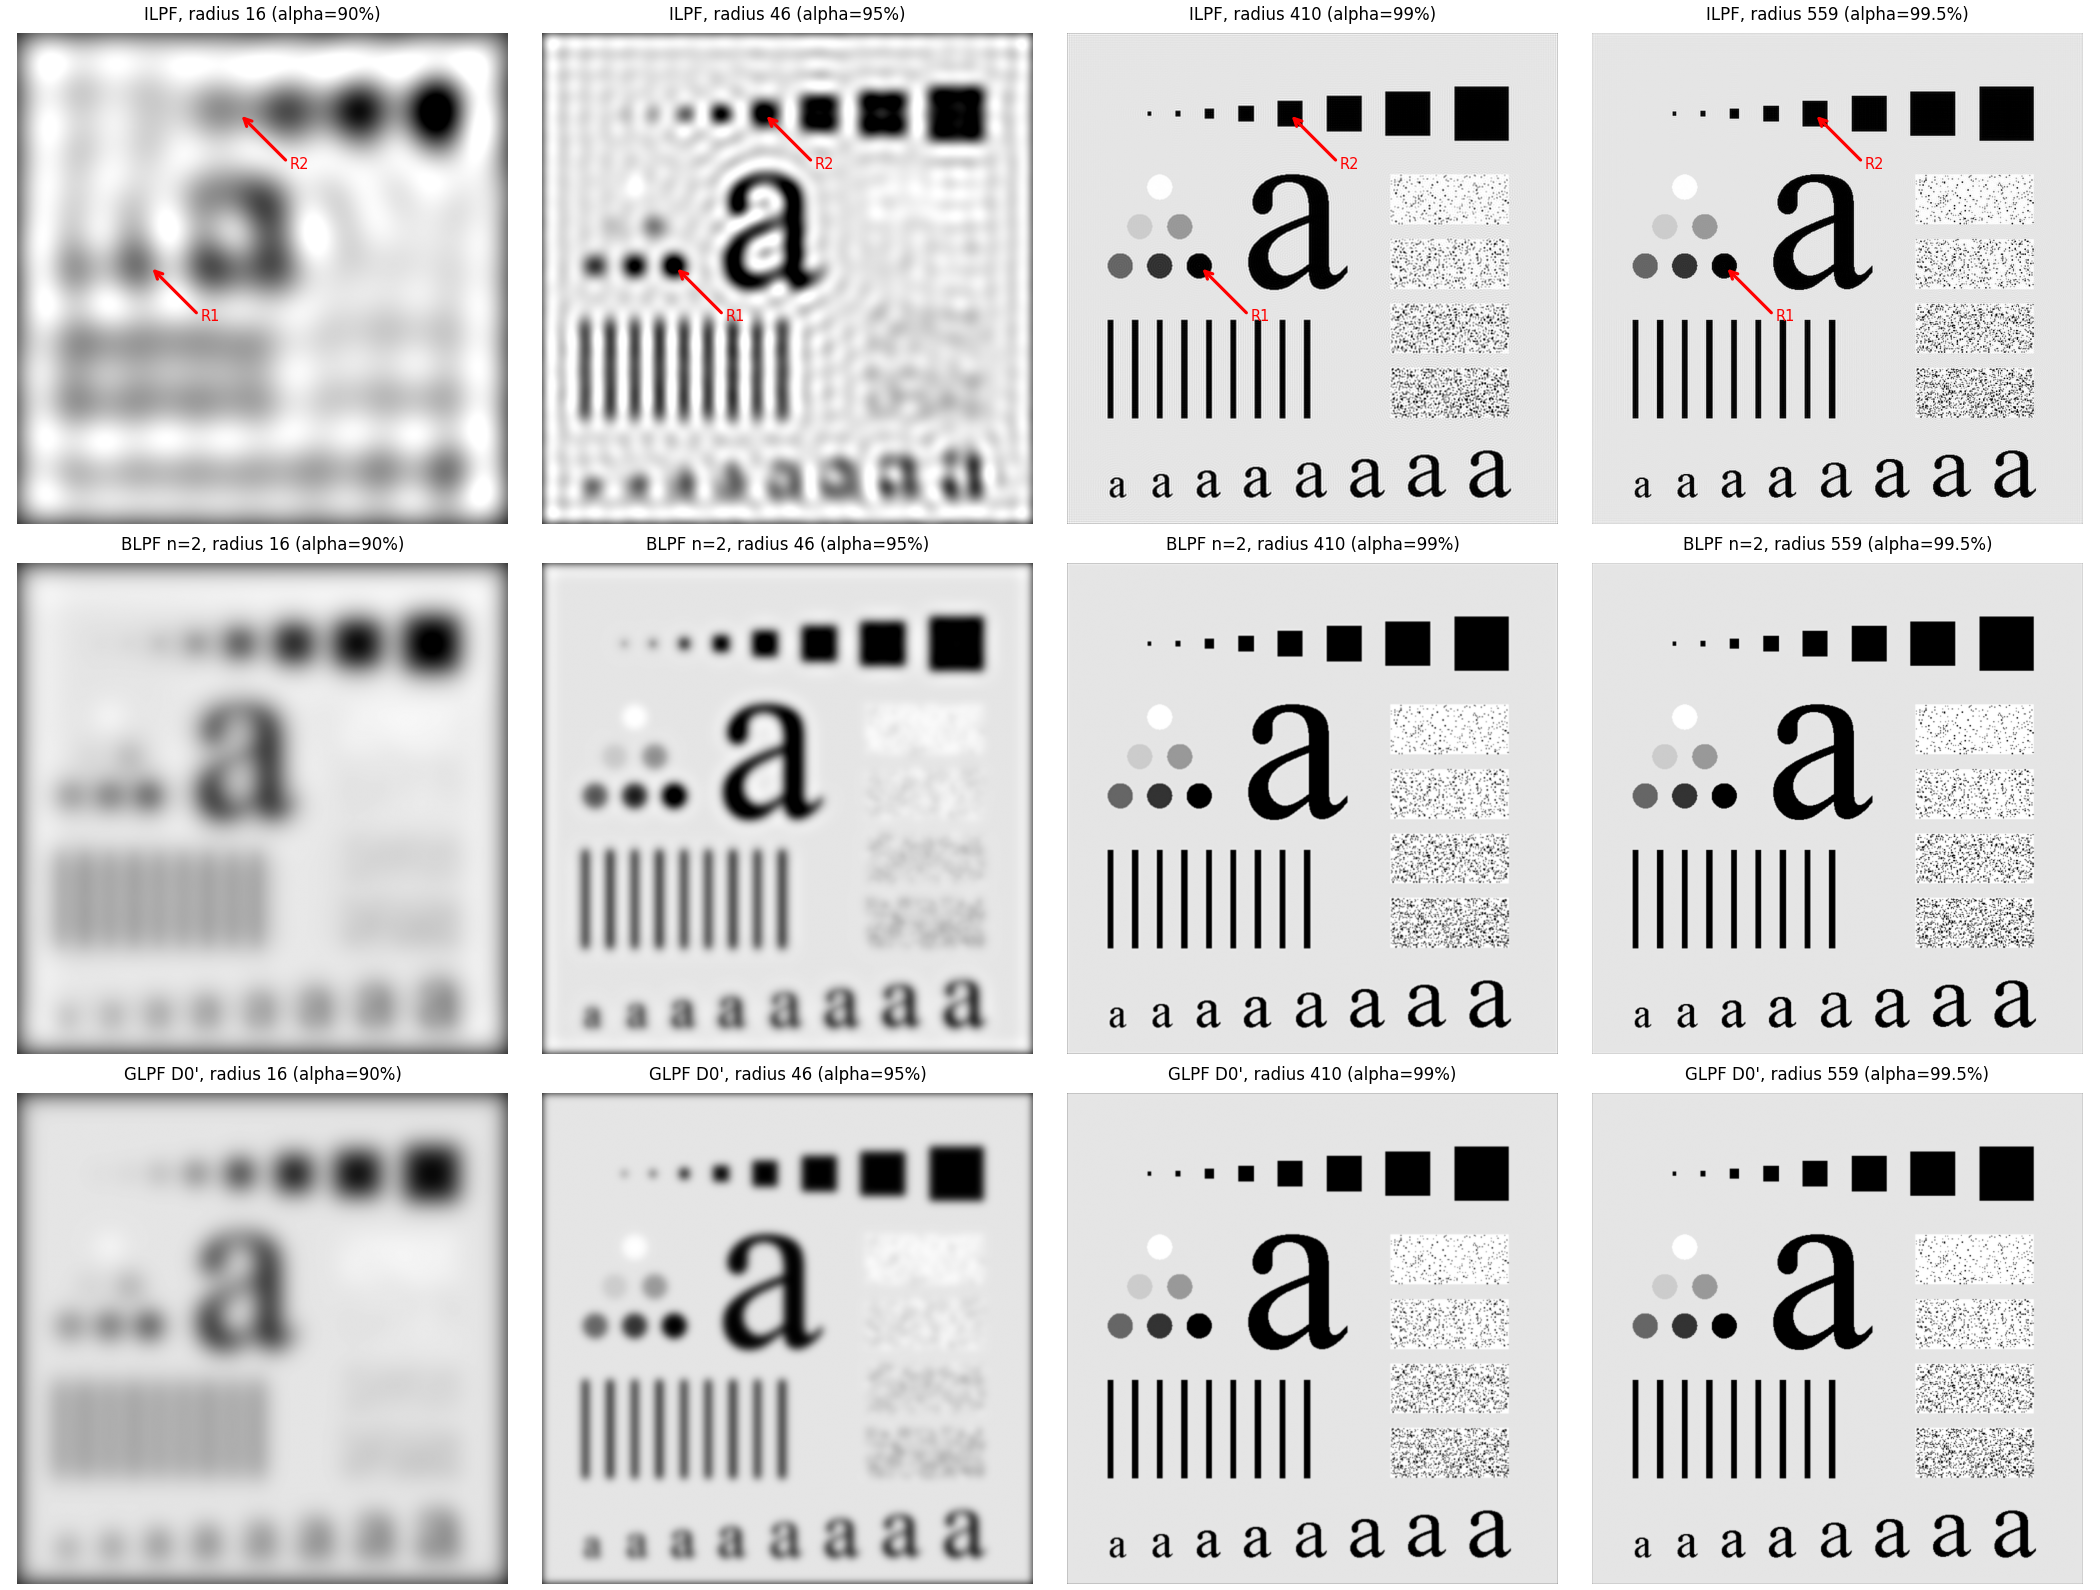
\includegraphics[width=1.00\linewidth]{q2_visual_grid}\par\vskip 3pt{\small\textbf{Figure 2.4.} Filter type (rows: ILPF, BLPF n=2, GLPF with matched D0') versus cutoff (columns: the radii enclosing 90, 95, 99, 99.5\% of the power). Red arrows R1, R2: ringing locations.\par}\end{figure}
\begin{figure}[H]\centering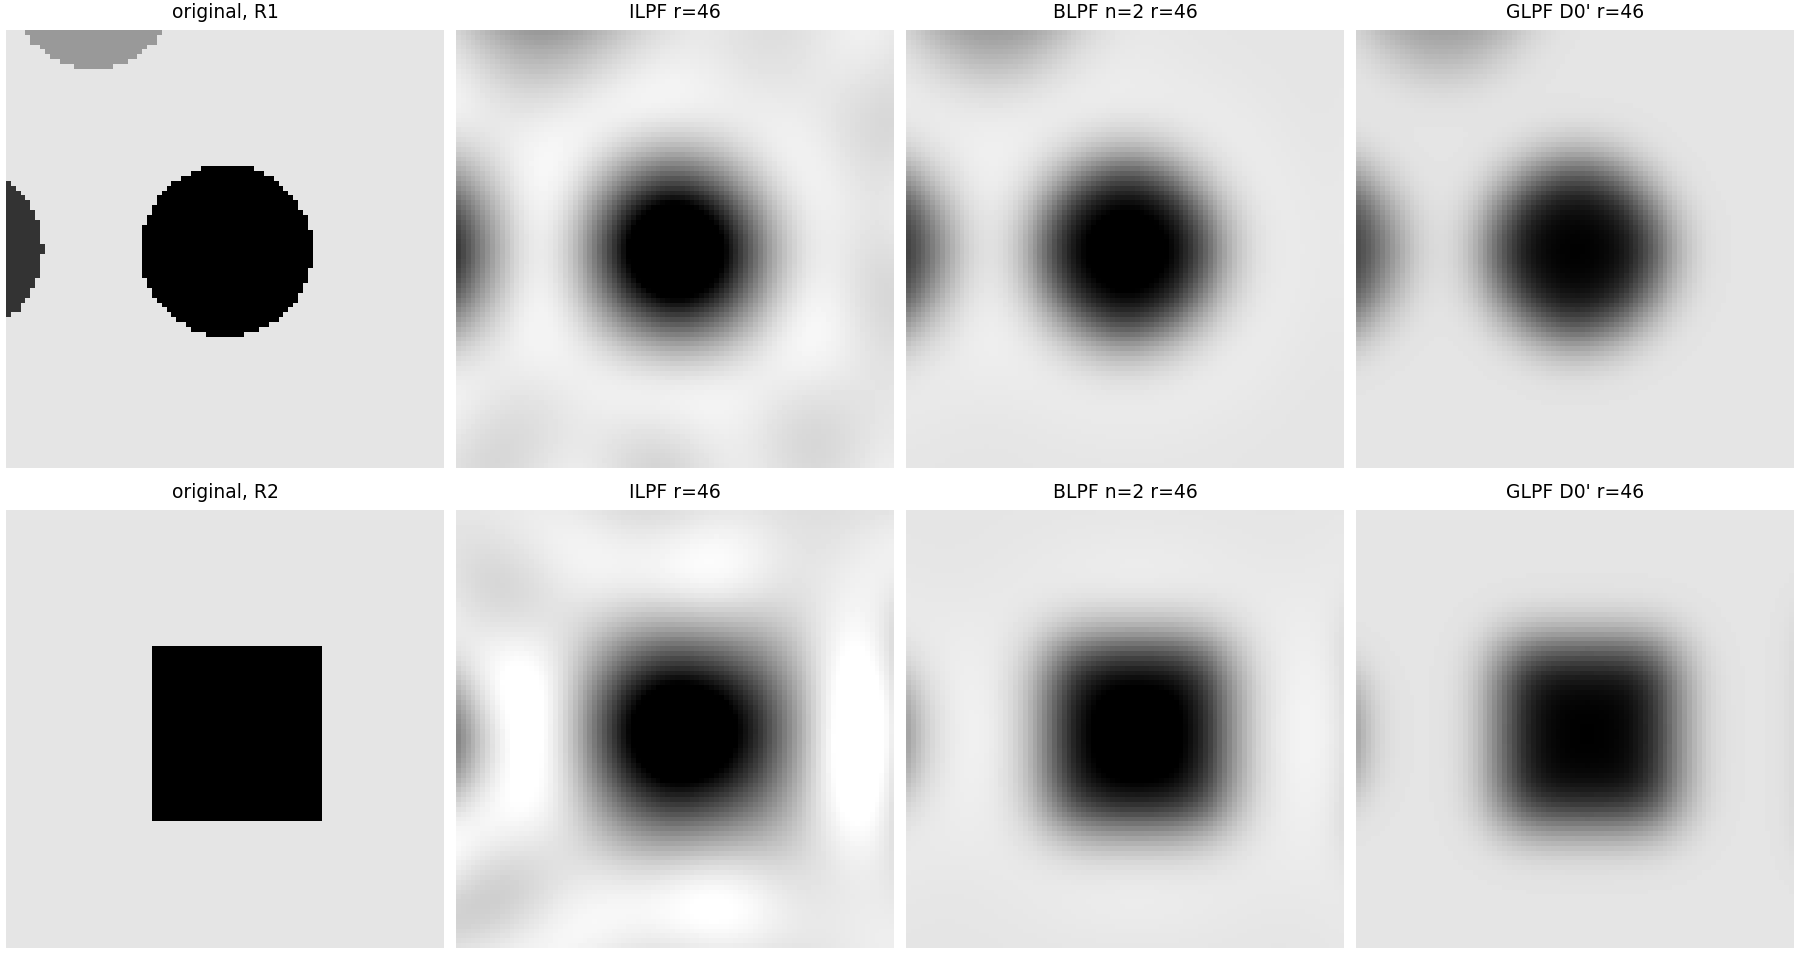
\includegraphics[width=0.90\linewidth]{q2_ringing_insets}\par\vskip 3pt{\small\textbf{Figure 2.5.} Zoomed insets at R1 and R2 (original, ILPF, BLPF n=2, GLPF) at D0 = 46: ripples in the ideal case only (faint overshoot for n=2, none for the Gaussian).\par}\end{figure}
\begin{table}[H]\centering\footnotesize{\small\textbf{Table 2.7.} RMS error of the filtered image relative to the original and [min, max] of the output (the original range is [0,255]; values outside it are pure ringing overshoot).\par}\vskip 3pt
\resizebox{\ifdim\width>\linewidth\linewidth\else\width\fi}{!}{\begin{tabular}{lrrrr}\toprule
\textbf{filter} & \textbf{radius 16} & \textbf{radius 46} & \textbf{radius 410} & \textbf{radius 559}\\\midrule
ILPF & 63.9 [-69, 286] & 46.5 [-90, 291] & 21.5 [-107, 364] & 15.2 [-134, 416]\\
BLPF n=2 & 60.4 [-15, 247] & 44.2 [-28, 258] & 17.4 [-31, 272] & 11.6 [-46, 292]\\
GLPF D0' & 60.8 [8, 245] & 44.5 [0, 255] & 17.2 [-5, 262] & 12.0 [-16, 273]\\
\bottomrule\end{tabular}}\end{table}
\textbf{Sharpness-ringing trade-off.} At any cutoff the ideal filter retains the sharpest transitions but produces the strongest ringing (output pushed to $[-134,416]$ at $D_0=559$ against $[-16,273]$ for the Gaussian); the Butterworth filter ($n=2$) is intermediate (about 4\% overshoot, one weak ripple); the Gaussian is monotone but gives the widest transitions for the same half-amplitude radius. RMS errors against the original are lowest for the Gaussian/Butterworth at 410 and 559 because the ILPF's ripples add error even where the passband is nearly everything; at 16 and 46 all three are blurred and the ILPF is additionally disturbed by ripples that look like a texture of the glyphs themselves (e.g. 'ghost' squares in the flat area).

\subsection{2.2d Gaussian equivalence check}
A spatial Gaussian $g(x)=\frac{1}{\sqrt{2\pi}\sigma_s}e^{-x^2/(2\sigma_s^2)}$ has transfer function $e^{-2\pi^2\sigma_s^2 f^2}$ with $f$ in cycles/pixel. On a $P$-point grid $f=k/P$ with $k=u-P/2$ the frequency-domain filter is $e^{-k^2/(2D_0^2)}$, so $2\pi^2\sigma_s^2/P^2=1/(2D_0^2)$:

\begin{equation}\sigma_s=\frac{P}{2\pi D_0}\end{equation}
\begin{table}[H]\centering\footnotesize{\small\textbf{Table 2.8.} cameraman.tif (P=1024): max \textbar{}g\_freq - g\_spatial\textbar{} (grey levels, 0-255 scale) against scipy.ndimage.gaussian\_filter with sigma\_s = P/(2 pi D0): default truncation at 4 sigma with zero boundary (mode='constant'), truncation at 8 sigma, and 8 sigma on the zero-padded periodic P x P array (isolating the kernel sampling difference).\par}\vskip 3pt
\resizebox{\ifdim\width>\linewidth\linewidth\else\width\fi}{!}{\begin{tabular}{rrrrrr}\toprule
\textbf{D0} & \textbf{sigma\_s (px)} & \textbf{H at Nyquist} & \textbf{\begin{tabular}[b]{@{}c@{}}err\\{}(truncate 4,\\{}zero bdry)\end{tabular}} & \textbf{\begin{tabular}[b]{@{}c@{}}err\\{}(truncate 8,\\{}zero bdry)\end{tabular}} & \textbf{\begin{tabular}[b]{@{}c@{}}err\\{}(truncate 8,\\{}periodic)\end{tabular}}\\\midrule
10 & 16.297 & 0.00e+00 & 1.25e-02 & 3.98e-13 & 3.98e-13\\
40 & 4.074 & 2.65e-36 & 1.64e-02 & 1.42e-13 & 1.42e-13\\
160 & 1.019 & 5.98e-03 & 6.92e-02 & 6.98e-02 & 6.98e-02\\
\bottomrule\end{tabular}}\end{table}
The error is not exactly zero for two reasons. (1) \textit{Kernel truncation}: \texttt{gaussian\_\allowbreak{}filter} cuts the kernel at 4$\sigma_s$ (mass $\mathrm{erfc}(4/\sqrt2)=6.3\times10^{-5}$ lost per axis, giving the $10^{-2}$ errors of column 4 for $D_0=10,40$); with truncation at 8$\sigma_s$ the two agree to $10^{-13}$, which confirms the derivation of $\sigma_s$ and the pipeline (zero padding $\equiv$ \texttt{mode=\allowbreak{}'constant'}). (2) \textit{Grid sampling}: the frequency-domain filter is band-limited at the Nyquist frequency (it only exists for $|k|\le P/2$), whereas the spatial Gaussian sampled on the pixel grid is aliased; the discrepancy is controlled by the Gaussian's value at Nyquist, $e^{-(P/2)^2/(2D_0^2)}$, which is $0$ for $D_0=10,40$ but $5.98e-03$ for $D_0=160$ ($\sigma_s=1.02$ px). Hence the error \textbf{grows with }$D_0$ and is not reduced by a longer kernel (0.0698 at $D_0=160$ with either truncation): a Gaussian narrower than about one pixel is not representable on the grid.

\subsection{2.3a Noise-blur trade-off}
Zero-mean Gaussian noise with $\sigma=20$ (seed 2026, drawn with \texttt{numpy.\allowbreak{}random.\allowbreak{}default\_\allowbreak{}rng(\allowbreak{}2026)}, \textbf{not clipped}) was added to cameraman.tif (PSNR of the noisy input: 22.46 dB, SSIM 0.327). PSNR (clipping the output to [0,255] for the metric) was evaluated against the clean image for $D_0=5..150$ (as required) and, because all three curves are still rising at $D_0=150$, for $D_0$ up to 300 so that the true optimum is found; for the Gaussian the sweep parameter is the half-amplitude radius $D_0$ with $D_0'=D_0/\sqrt{2\ln2}$.

\begin{figure}[H]\centering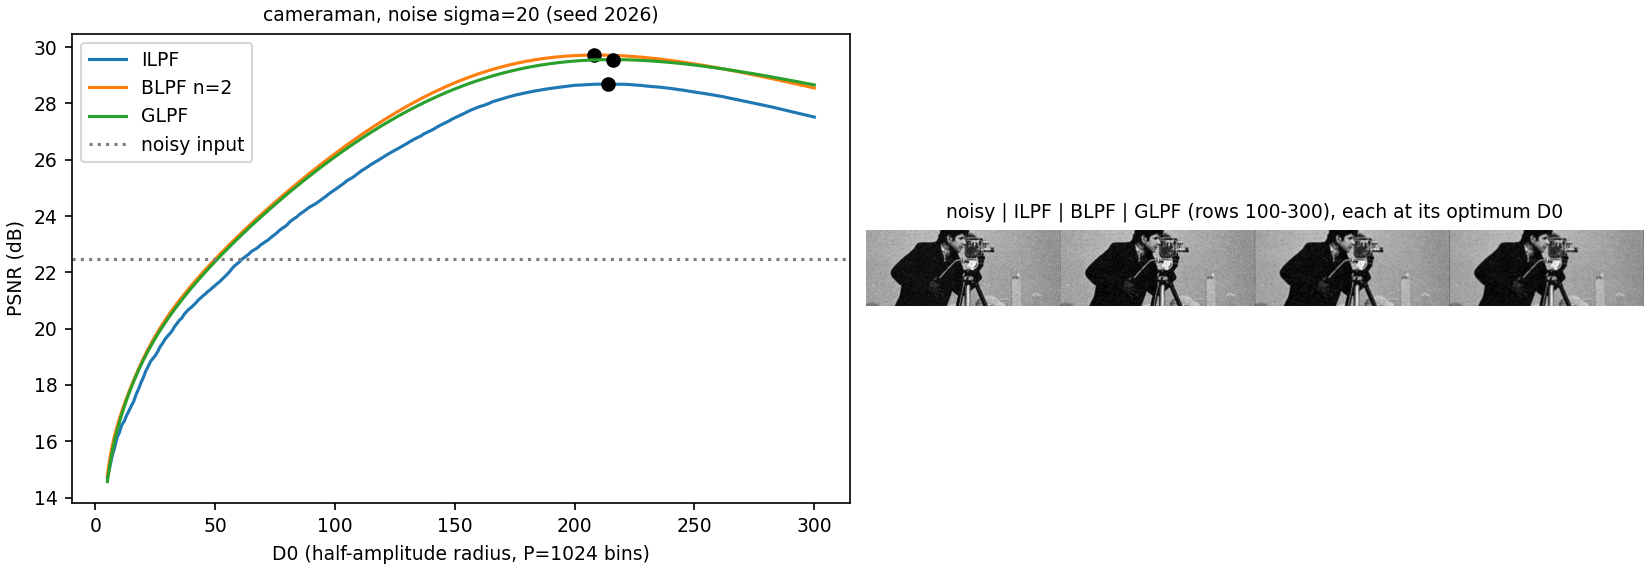
\includegraphics[width=1.00\linewidth]{q2_psnr_sweep}\par\vskip 3pt{\small\textbf{Figure 2.6.} PSNR vs D0 for the three low-pass families on one plot (noise sigma=20, seed 2026); dots mark each optimum. Right: the three outputs at their optimum.\par}\end{figure}
\begin{table}[H]\centering\footnotesize{\small\textbf{Table 2.9.} Optimal cutoff and peak PSNR. Columns 2-3: best D0 inside the required range 5..150 (at the edge of the range for every family); columns 4-6: optimum of the extended sweep (D0 \textless{}= 300, step 2 beyond 150) with PSNR and SSIM.\par}\vskip 3pt
\resizebox{\ifdim\width>\linewidth\linewidth\else\width\fi}{!}{\begin{tabular}{lrrrrr}\toprule
\textbf{family} & \textbf{\begin{tabular}[b]{@{}c@{}}best D0 in\\{}5..150\end{tabular}} & \textbf{PSNR (dB)} & \textbf{\begin{tabular}[b]{@{}c@{}}best D0\\{}(extended)\end{tabular}} & \textbf{\begin{tabular}[b]{@{}c@{}}peak PSNR\\{}(dB)\end{tabular}} & \textbf{\begin{tabular}[b]{@{}c@{}}SSIM at\\{}optimum\end{tabular}}\\\midrule
ILPF & 150 & 27.49 & 214 & 28.69 & 0.700\\
BLPF n=2 & 150 & 28.73 & 208 & 29.72 & 0.761\\
GLPF & 150 & 28.52 & 216 & 29.56 & 0.753\\
\bottomrule\end{tabular}}\end{table}
\textbf{Interpretation.} Noise is white (flat spectrum, power $\sigma^2$) while the image power falls rapidly with frequency, so a low-pass trades removed noise power (proportional to the passband \textit{area}, $\propto D_0^2$) against removed signal power (the image energy beyond $D_0$). Small $D_0$ blurs the image (signal loss dominates), large $D_0$ passes almost all noise; the maximum is where marginal noise power equals marginal signal power: near $D_0\approx 210$ bins ($0.2$ cycles/pixel, i.e. about 40\% of Nyquist), where the cameraman's spectrum has fallen to the noise floor. The Butterworth and Gaussian filters peak slightly higher than the ILPF because their smooth roll-off attenuates the transition band gradually; the ideal filter's abrupt cutoff gives a sinc kernel with slowly decaying side lobes, i.e. ringing (the added error) that remains even at the optimum, so it has the lowest peak (28.69 dB vs 29.72 / 29.56 dB; its SSIM 0.700 is also clearly lower). The Butterworth ($n=2$) is the best of the three here (+1.03 dB over ILPF): it keeps a flatter passband than the Gaussian (whose attenuation already reaches $e^{-1/2}$ at $D_0'$ and 0.5 at $D_0$) while still rolling off smoothly, and the two optima are within 0.16 dB.

\subsection{2.3b Character repair}
text\_gaps.tif (444x508, padded to P=1016) contains 1-2 pixel gaps in the glyph strokes. A Gaussian low-pass was swept and a proxy was computed: the number of 8-connected components of dark pixels (\textless{} 127.5) - the original has 266, many being broken stroke fragments - together with the dark area fraction (Table 2.10). The proxy alone cannot choose $D_0$ (a very small $D_0$ yields one component, because everything merges into a grey smear); it was combined with visual inspection of Figure 2.7.

\begin{table}[H]\centering\small{\small\textbf{Table 2.10.} Gaussian LPF sweep on text\_gaps.tif (parameter = Gaussian D0 on the P=1016 grid).\par}\vskip 3pt
\resizebox{\ifdim\width>\linewidth\linewidth\else\width\fi}{!}{\begin{tabular}{rrrr}\toprule
\textbf{D0 (Gaussian)} & \textbf{dark components} & \textbf{dark area \%} & \textbf{min grey level}\\\midrule
10 & 1 & 1.25 & 60.6\\
15 & 1 & 1.01 & 59.1\\
20 & 1 & 0.94 & 57.6\\
30 & 1 & 0.88 & 54.7\\
40 & 1 & 0.86 & 51.8\\
50 & 1 & 0.86 & 49.0\\
60 & 23 & 0.91 & 46.3\\
70 & 100 & 1.22 & 43.6\\
80 & 209 & 1.85 & 41.1\\
90 & 338 & 2.93 & 38.6\\
100 & 372 & 4.15 & 36.2\\
120 & 313 & 5.93 & 25.5\\
160 & 264 & 7.22 & 5.3\\
\bottomrule\end{tabular}}\end{table}
\begin{figure}[H]\centering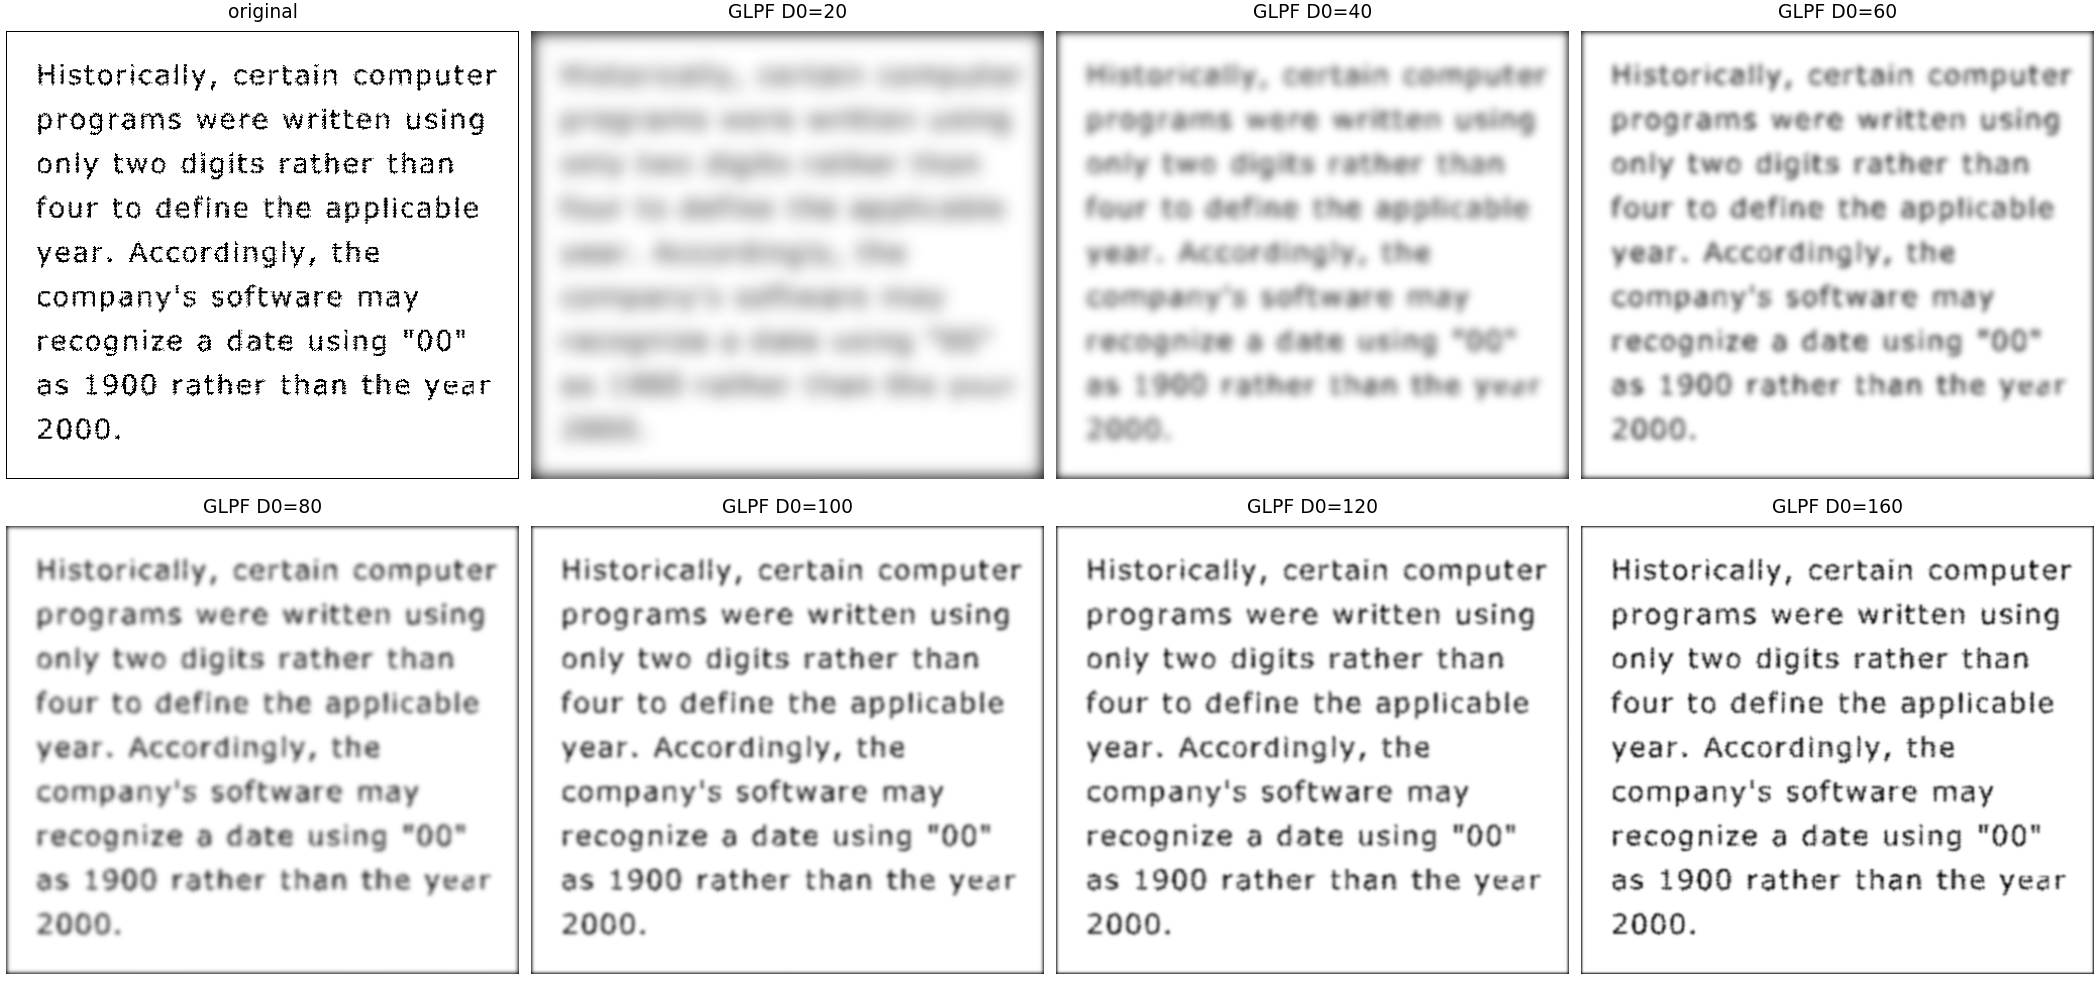
\includegraphics[width=1.00\linewidth]{q2_text_sweep}\par\vskip 3pt{\small\textbf{Figure 2.7.} Gaussian low-pass sweep on text\_gaps.tif. Below D0\textasciitilde{}60 the words are smeared; D0\textasciitilde{}80 joins the broken strokes while the characters remain legible; at D0=160 the gaps are still visible.\par}\end{figure}
\begin{figure}[H]\centering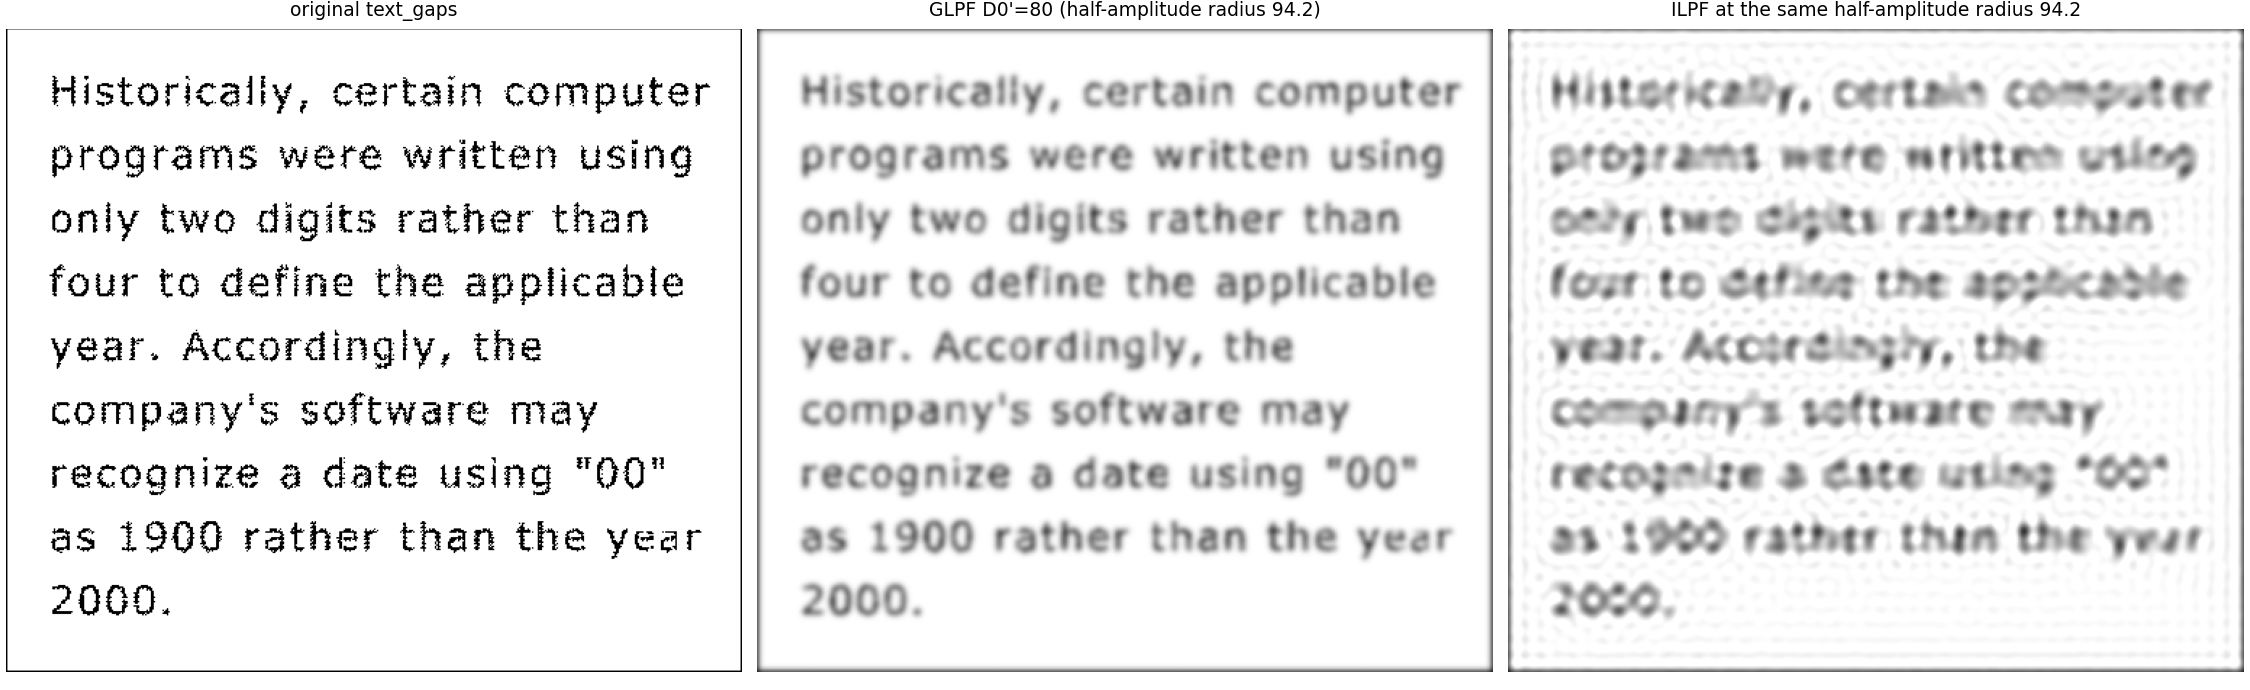
\includegraphics[width=1.00\linewidth]{q2_text_repair}\par\vskip 3pt{\small\textbf{Figure 2.8.} Chosen repair: Gaussian D0' = 80 (half-amplitude radius 94.2) next to the ideal filter with the same half-amplitude radius.\par}\end{figure}
\begin{figure}[H]\centering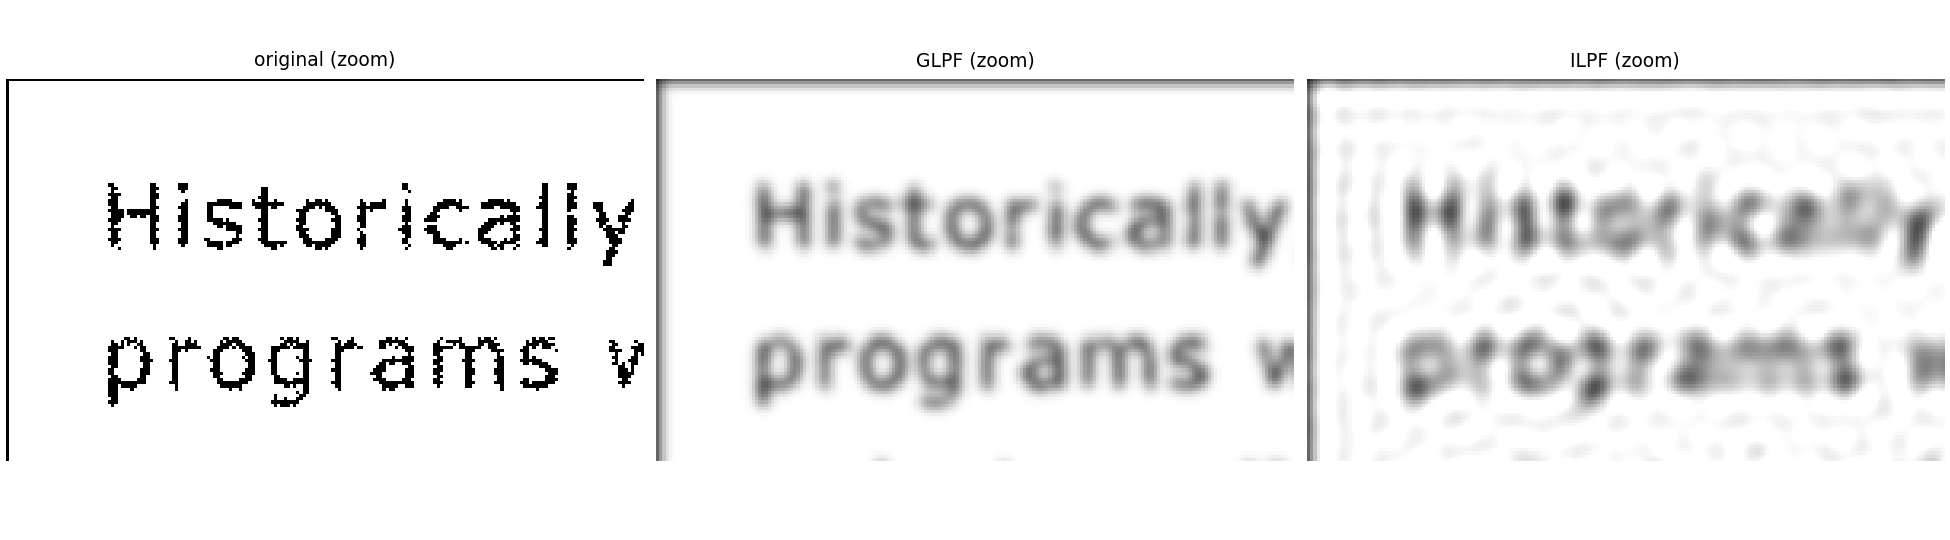
\includegraphics[width=1.00\linewidth]{q2_text_repair_zoom}\par\vskip 3pt{\small\textbf{Figure 2.9.} Zoom of the top-left region: original, GLPF D0'=80, ILPF at radius 94.2.\par}\end{figure}
\textbf{Choice: Gaussian }$D_0'=80$ (half-amplitude radius $94.2$ bins; spatial $\sigma_s=P/(2\pi D_0')=2.02$ px, so the gap of 1-2 px is spanned by one standard deviation of the kernel). At $D_0'=60$ the components drop to 23 and neighbouring letters merge ('words' become blobs, minimum grey level 46 - the text is unreadable); at $D_0'\ge100$ between 264 and 372 components remain and the gaps are visible. At $D_0'=80$ the number of components falls from 266 to 209: the broken strokes are joined (the remaining components are separate letters and dots) while counters of letters such as 'a' and 'e' are still open. \textbf{Ideal filter at the same half-amplitude radius:} it reaches 193 components too (it also bridges gaps), but its sinc kernel produces ringing: the output ranges over [38, 318] instead of [41, 255], the glyphs are surrounded by parallel ripples, and the ripples create faint false strokes in the white background (RMS difference from the Gaussian result 14.8 grey levels). The Gaussian never overshoots (non-negative kernel).

\subsection{2.3c High-pass filtering, the DC term and high-frequency emphasis}
thumb\_print.tif (962x1026, $P=2052$) was filtered with IHPF, BHPF ($n=4$) and GHPF at a common half-amplitude radius $D_0=60$ bins (GHPF: $D_0'=51.0$).

\begin{table}[H]\centering\footnotesize{\small\textbf{Table 2.11.} High-pass outputs on thumb\_print.tif (input mean 142.73). H\_HP(P/2,P/2) is the DC gain; 'mean (cropped)' is the mean of the cropped 962x1026 output; 'mean (padded)' the mean over the whole PxP output.\par}\vskip 3pt
\resizebox{\ifdim\width>\linewidth\linewidth\else\width\fi}{!}{\begin{tabular}{lrrrrrr}\toprule
\textbf{filter} & \textbf{H\_HP(DC)} & \textbf{\begin{tabular}[b]{@{}c@{}}mean\\{}(cropped\\{}output)\end{tabular}} & \textbf{\begin{tabular}[b]{@{}c@{}}mean (full\\{}padded PxP)\end{tabular}} & \textbf{std} & \textbf{min} & \textbf{max}\\\midrule
IHPF & 0 & 1.195 & 2.76e-17 & 31.32 & -116.3 & 157.1\\
BHPF n=4 & 0 & 1.220 & 4.15e-17 & 30.51 & -107.1 & 157.8\\
GHPF & 0 & 1.725 & 5.53e-17 & 28.79 & -95.8 & 157.5\\
\bottomrule\end{tabular}}\end{table}
All three high-pass filters have $H_{HP}(P/2,P/2)=1-H_{LP}(0)=0$: the DC term is removed. The mean of the output over the full padded array is $\hat f_{pad}[\,]=H(0)\cdot\frac1{P^2}F(0,0)=0$ exactly (measured $\sim10^{-17}$, Table 2.11); the mean of the \textit{cropped} output is not exactly zero (1.2-1.7 grey levels, against an input mean of 142.7) because the crop discards the filtered padded region, where the filter output ($\approx$ minus a smoothed copy of the image edge) has the opposite sign. The tonal information (the overall brightness and slow shading) is lost: the high-pass image is zero-mean with ridges as positive/negative excursions.

\textbf{High-frequency emphasis} $H_{HFE}=k_1+k_2H_{HP}$ with $k_1=1$, $k_2=0.5$ (and the Gaussian high-pass above): the DC gain is $k_1=1$ (so tone is preserved: output mean 143.6 vs input 142.7, ratio 1.006), the gain at high frequencies is $k_1+k_2=1.5$, and the local contrast of ridges (mean standard deviation in 15x15 windows) rises from 27.4 to 39.9 (x1.46) while 1.9\% of pixels leave $[0,255]$ (clipped for display; $k_2=1.5$ would clip 12\%, so the milder setting was chosen). Figure 2.10 shows the original, the three high-pass outputs, the emphasised image and the Otsu-thresholded binary ridge maps; Figure 2.11 is a zoomed crop.

\begin{figure}[H]\centering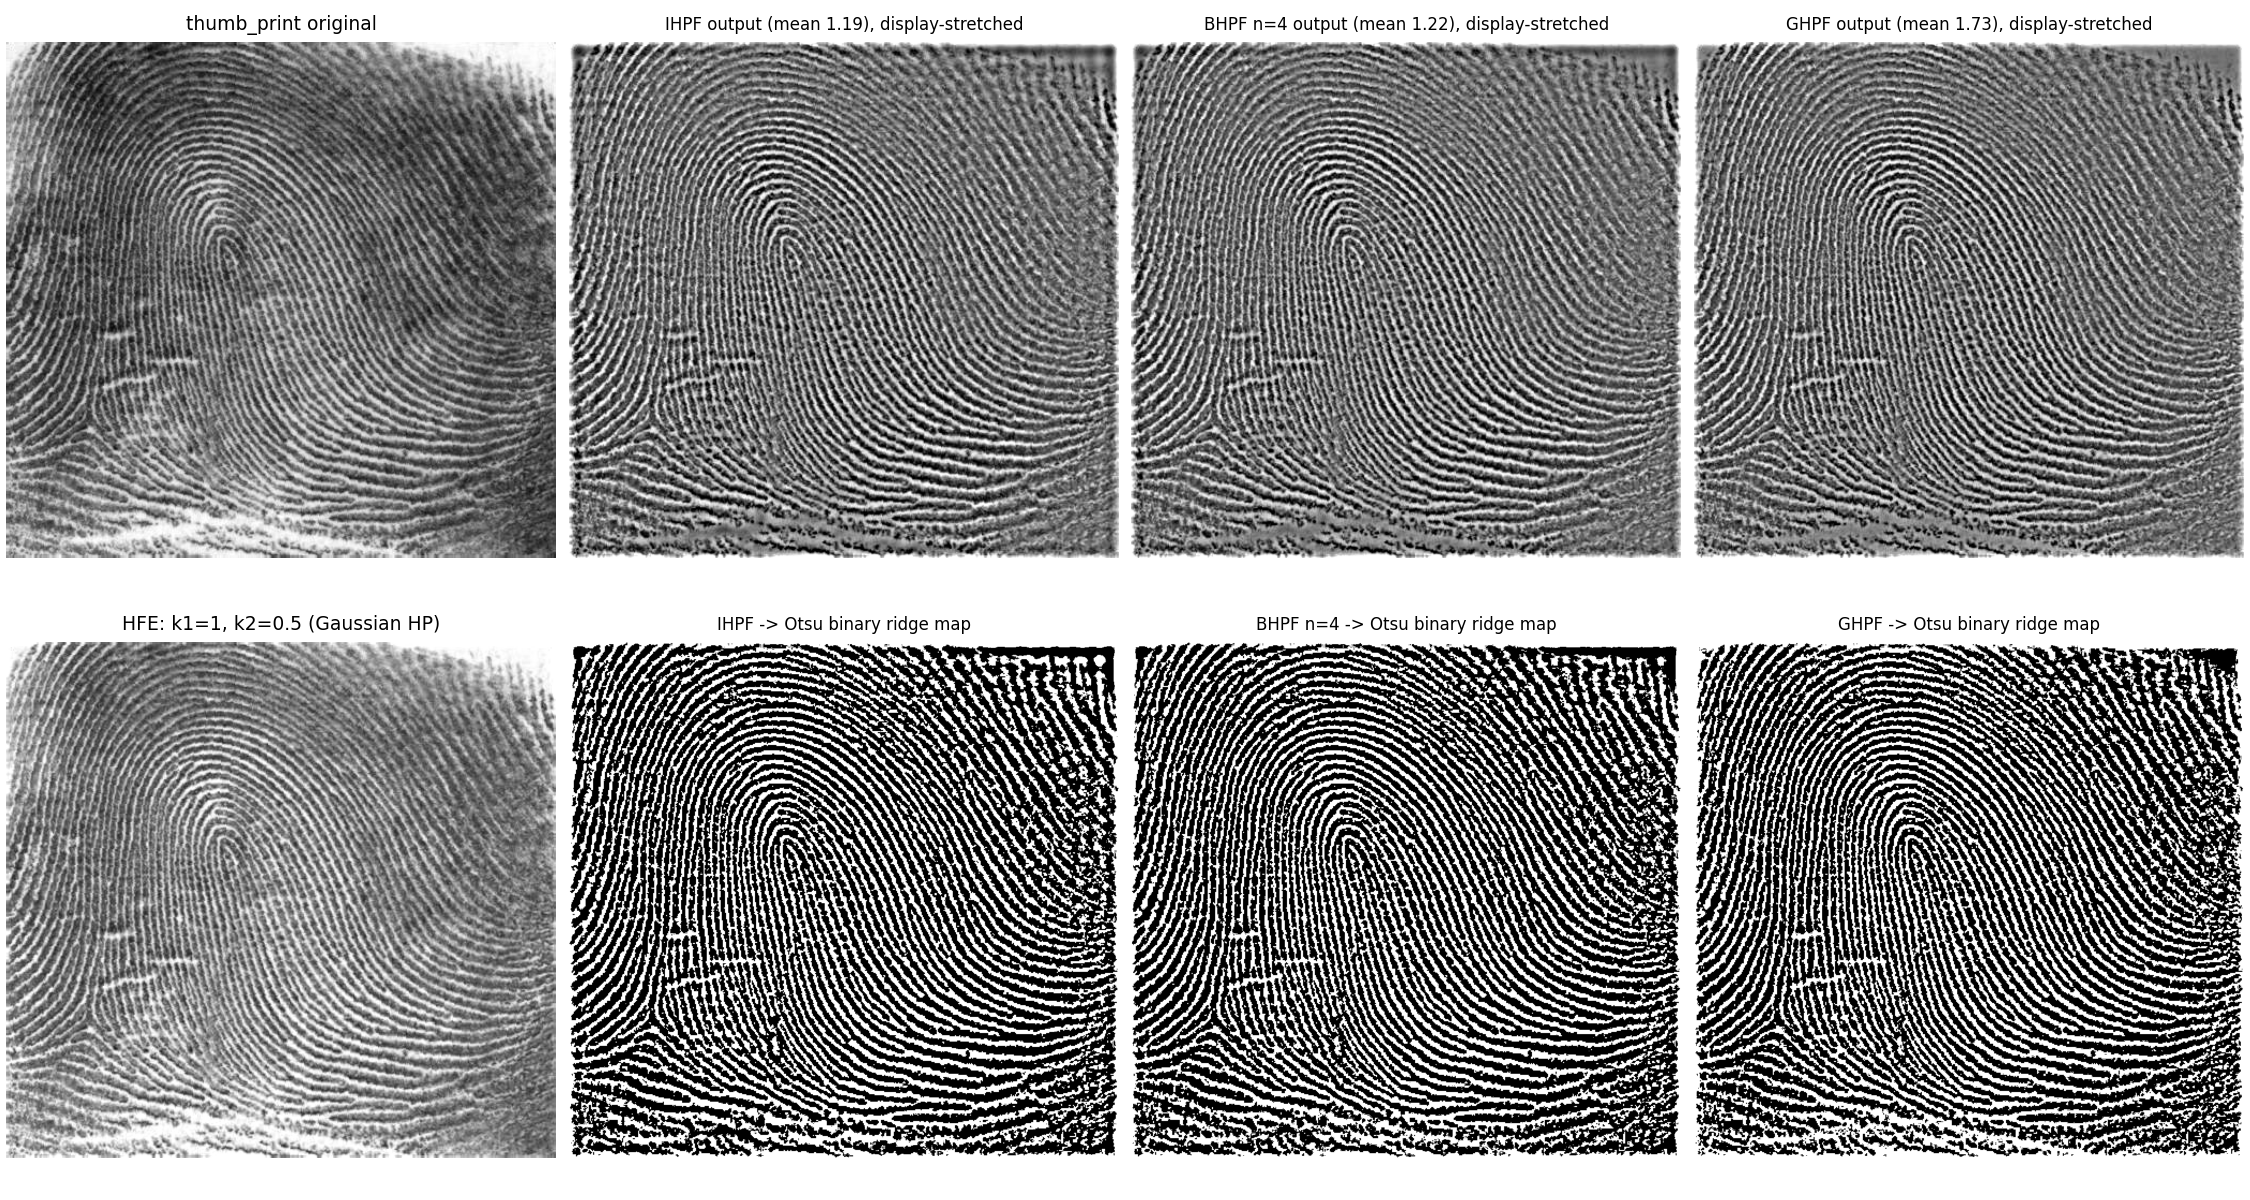
\includegraphics[width=1.00\linewidth]{q2_highpass}\par\vskip 3pt{\small\textbf{Figure 2.10.} Top: original and the IHPF/BHPF/GHPF outputs (display stretched; means are \textasciitilde{}1). Bottom: high-frequency emphasis (k1=1, k2=0.5) and Otsu-thresholded binary ridge maps.\par}\end{figure}
\begin{figure}[H]\centering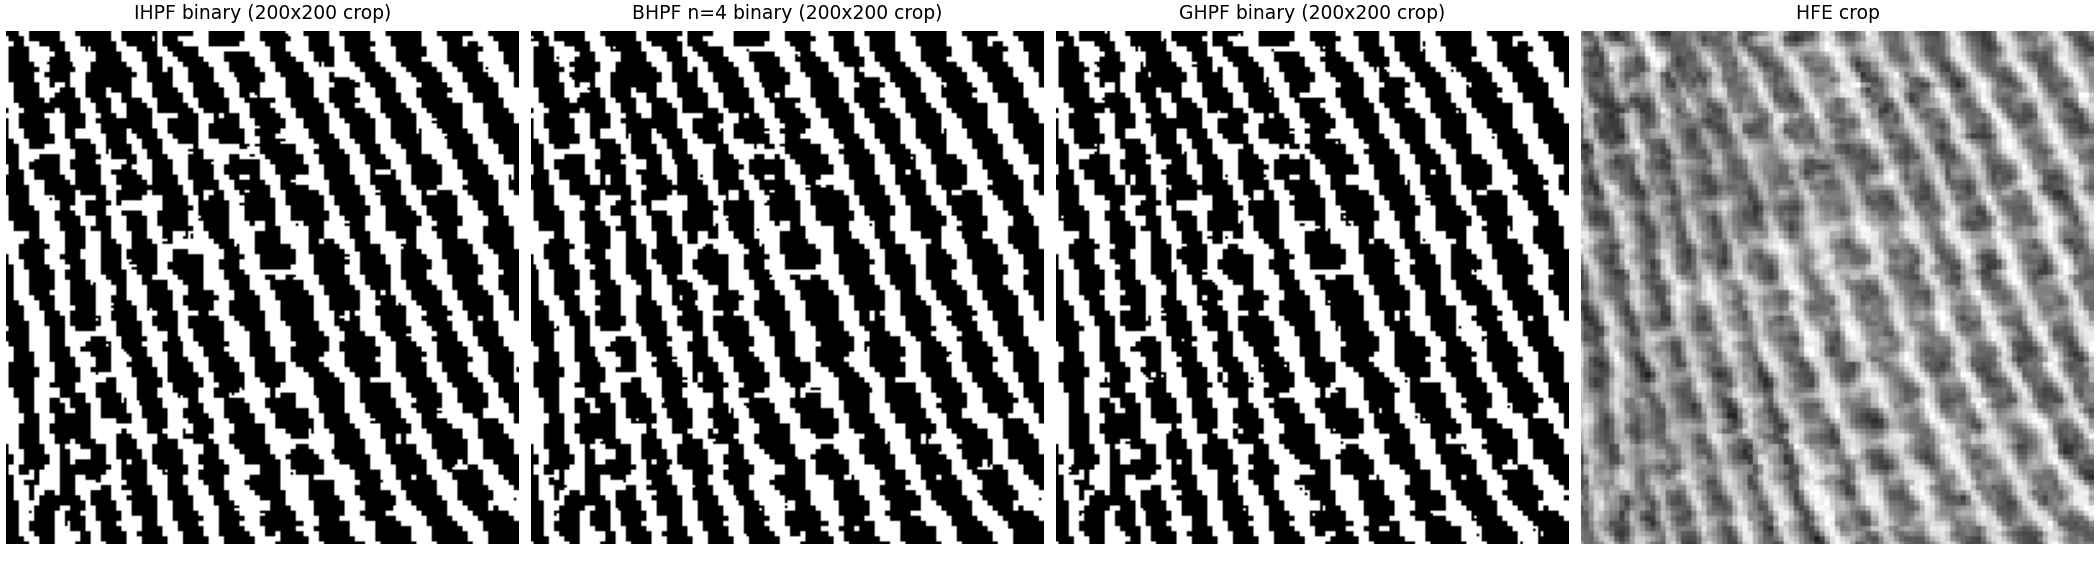
\includegraphics[width=1.00\linewidth]{q2_highpass_crops}\par\vskip 3pt{\small\textbf{Figure 2.11.} 200x200 crops of the three binary ridge maps and of the HFE image.\par}\end{figure}
\begin{table}[H]\centering\footnotesize{\small\textbf{Table 2.12.} Binary ridge maps (Otsu threshold of each high-pass output).\par}\vskip 3pt
\resizebox{\ifdim\width>\linewidth\linewidth\else\width\fi}{!}{\begin{tabular}{lrrrrr}\toprule
\textbf{filter} & \textbf{\begin{tabular}[b]{@{}c@{}}Otsu\\{}threshold\end{tabular}} & \textbf{foreground \%} & \textbf{components} & \textbf{\begin{tabular}[b]{@{}c@{}}components \textless{}\\{}20 px\end{tabular}} & \textbf{\begin{tabular}[b]{@{}c@{}}tiny per\\{}10\textasciicircum{}4 px\end{tabular}}\\\midrule
IHPF & 5.95 & 40.6 & 1167 & 926 & 9.38\\
BHPF n=4 & 6.18 & 40.1 & 1307 & 1025 & 10.38\\
GHPF & 5.63 & 41.1 & 1738 & 1467 & 14.86\\
\bottomrule\end{tabular}}\end{table}
\textbf{Which filter gives the cleanest ridges?} In this experiment the three maps are visually almost identical (Figure 2.11); the counts of isolated tiny components (a proxy for speckle) are IHPF 926 \textless{} BHPF 1025 \textless{} GHPF 1467. The difference is small and not what the textbook intuition suggests ('Butterworth is the cleanest'). The explanation consistent with the transfer functions: at a common half-amplitude radius the Gaussian high-pass rises most slowly, so it passes least of the low-frequency ridge band near the cutoff and relatively more of the pixel-scale noise, whereas the ideal high-pass passes the ridge band completely but its sinc side lobes ring along the ridge direction (ringing is partly hidden because ridges are themselves quasi-periodic). The Butterworth filter is the compromise (no abrupt cutoff, little ringing, steep enough transition): it is the recommended choice in practice, but the quantitative evidence here shows only a marginal advantage of the sharper filters in speckle count and no decisive winner; the binary maps are limited more by the global Otsu threshold than by the filter.

\section{Question 3 - Homomorphic filtering: illumination and reflectance}
\subsection{3.1 The multiplicative model}
An image formed by a reflecting scene is modelled as $I(x,y)=L(x,y)\,R(x,y)$ with $0<R\le1$ the reflectance (fine detail, edges, texture; high spatial frequencies) and $L>0$ the illumination, assumed slowly varying (low frequencies, e.g. the falloff of a lamp, a vignette, the tunnel light). A linear frequency-domain filter cannot separate $L$ and $R$ directly because the Fourier transform of a product is the \textit{convolution} of the transforms, $\mathcal F\{LR\}=\mathcal F\{L\}\circledast\mathcal F\{R\}$: the two spectra overlap and smear into each other. The logarithm turns the product into a sum,

\begin{equation}z=\ln I=\ln L+\ln R\ \Rightarrow\ \mathcal F\{z\}=\mathcal F\{\ln L\}+\mathcal F\{\ln R\}\end{equation}
and now $\ln L$ (slowly varying) concentrates near the origin and $\ln R$ at higher frequencies, so a linear shift-invariant filter acting on $z$ can attenuate the first and boost the second; the exponential brings the result back to the intensity domain, $\hat I=\exp(\mathcal F^{-1}\{H\,\mathcal F\{z\}\})$. Numerically, $\ln(LR)$ and $\ln L+\ln R$ agree to 4.44e-16 on a synthetic illumination/reflectance pair (tests/test\_q3.py); a constant $\epsilon=1/255$ is added before the logarithm because real images contain exact zeros.

\textbf{Why the log must come before the Fourier transform.} Filtering is linear only in the domain where the model is additive. The pipeline $\ln\to\mathcal F\to H\to\mathcal F^{-1}\to\exp$ filters $\ln L$ and $\ln R$ separately. If instead we took the Fourier transform of $I$ and then the logarithm of its magnitude, we would obtain $\ln|\mathcal F\{L\}\circledast\mathcal F\{R\}|$, which does \textit{not} separate into a function of $L$ plus a function of $R$ (the log of a convolution of spectra has no additive structure), so there is no frequency band in which 'illumination' lives; moreover the log-magnitude discards the phase, so a filter on it cannot be inverted into an image at all, and $\ln|F|$ is dominated by the DC term and the $1/|k|^\alpha$ envelope of the whole image, not of the illumination. In short: filtering $\ln|\mathcal F\{I\}|$ is a \textit{spectral} operation on the magnitude, whereas the model requires a \textit{spatial} operation $\ln I$. Figure 3.1 shows the two spectra for the supplied image: the spectrum of $\ln I$ is much more concentrated near the origin (the slowly varying illumination), the spectrum of $I$ is dominated by the huge intensity step of the aperture.

\begin{figure}[H]\centering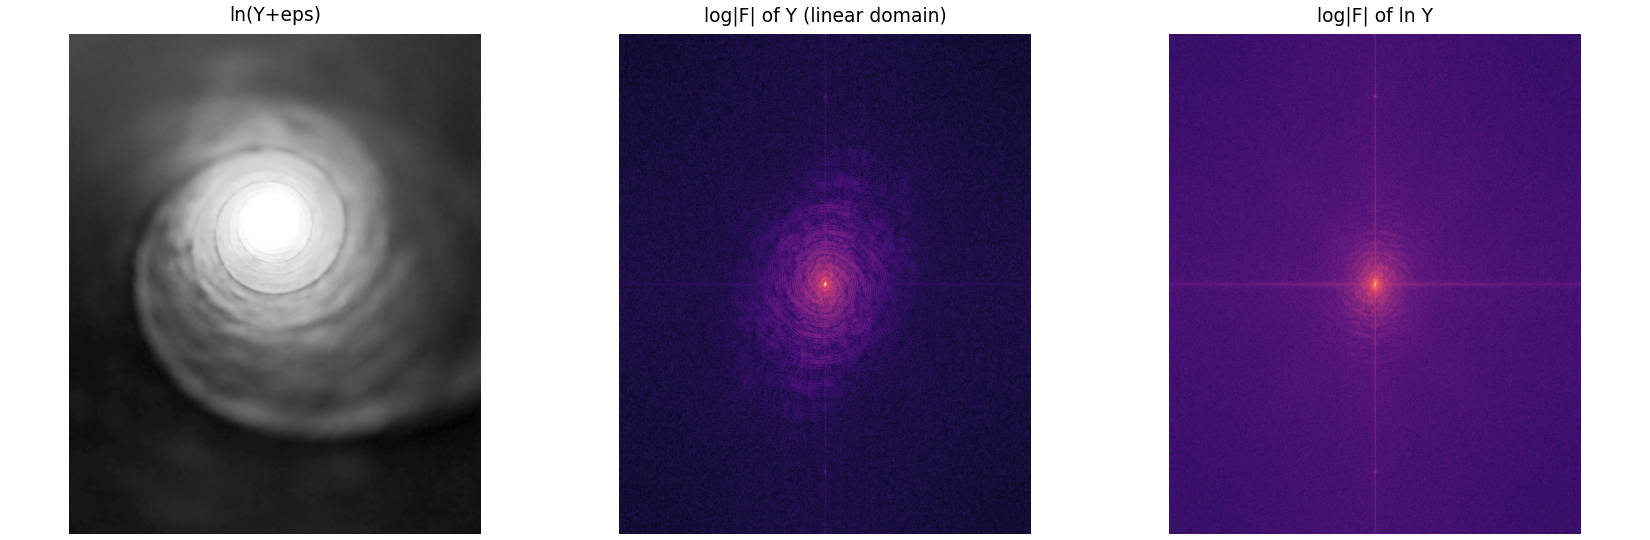
\includegraphics[width=0.95\linewidth]{q3_log_spectra}\par\vskip 3pt{\small\textbf{Figure 3.1.} ln(Y+eps) of the tunnel luminance and the log-magnitude spectra of Y (linear domain) and of ln Y.\par}\end{figure}
\subsection{3.2 Implementation and tuning}
\textbf{Data.} The provided photograph tunnel\_image.jpg (3000x3644, deep shadow in the tunnel walls, a saturated bright aperture; 1.17\% of the pixels are at 255 and the median luminance is 20.7/255) was reduced by 3x3 block averaging to 1000x1214 to keep the 2-D FFT sizes practical. Processing is applied to the BT.601 luminance $Y$; the colour of every output pixel is restored by scaling the RGB triple by $Y_{out}/Y_{in}$. Derived images are in \texttt{data/\allowbreak{}derived/\allowbreak{}}.

\begin{equation}H(u,v)=(\gamma_H-\gamma_L)\left[1-e^{-c\,D^{2}(u,v)/D_0^{2}}\right]+\gamma_L,\qquad \gamma_L<1<\gamma_H,\ c=1\end{equation}
$D$ is the radial frequency in cycles/pixel on the padded FFT grid (so $D_0$ is resolution independent: $D_0=0.02$ cycles/pixel means structures with a period of 50 px); the DC gain is $\gamma_L$ (illumination compressed), the high-frequency gain tends to $\gamma_H$ (reflectance boosted); with $\gamma_L=\gamma_H=1$ the filter is the identity (tested to $10^{-12}$). The log image is mirror-padded to about twice its size before the FFT (zero padding would create an artificial step in the log image) and cropped afterwards; the result is $\exp(\cdot)-\epsilon$ and is normalised by its 99.9th percentile (clipping to [0,1]).

\begin{figure}[H]\centering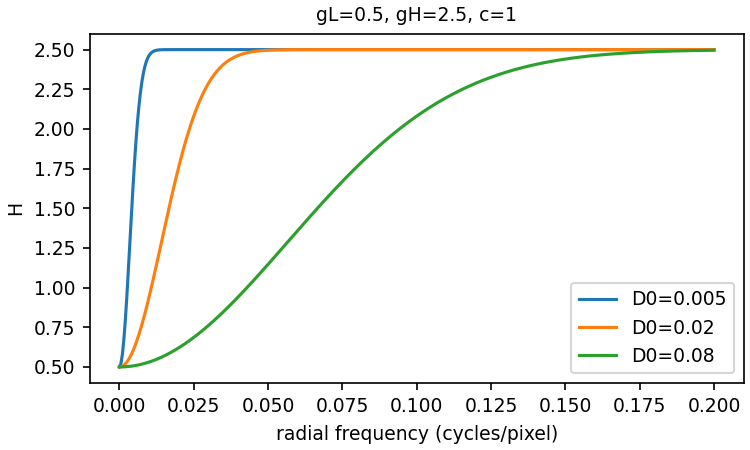
\includegraphics[width=0.45\linewidth]{q3_filter_profile}\par\vskip 3pt{\small\textbf{Figure 3.2.} Radial profile of the homomorphic filter for gamma\_L = 0.5, gamma\_H = 2.5 and three cutoffs.\par}\end{figure}
\textbf{Parameter sweep.} $\gamma_L\in\{0.25,0.5,0.75\}$, $\gamma_H\in\{1.5,2.5,4\}$, $D_0\in\{0.005,0.02,0.08\}$ cycles/pixel (27 settings; Figures 3.3-3.5: one 3x3 grid per $D_0$; cyan box = shadow region; red titles = halo flag). For every setting the code measures (i) \textit{illumination flattening}: ratio of the mean level in the shadow box to the mean level in the aperture disc (input 0.073); (ii) \textit{local contrast} in the shadow box: mean 9x9 local standard deviation, and the standard deviation of $\ln(Y+\epsilon)$ (scale-invariant, so it is not changed by global gain); (iii) the same measures in a \textit{detail-free control region} (deep black upper-left corner), to separate real detail from amplified noise and JPEG artefacts; (iv) saturation (fraction of pixels $\ge 0.98$); (v) a \textit{halo index}: the annular mean of $\ln Y$ about the aperture centre (radius $R_e=67$ px) is computed and the rim overshoot inside the aperture edge, $\max_{0.6R_e<r<R_e}p(r)-\overline p_{r<0.4R_e}$, is divided by the plateau-to-surround step $S$; values above 0.10 are flagged (the input and HE give $\le 10^{-16}$). The threshold is a heuristic; the grids show what it means visually.

\begin{figure}[H]\centering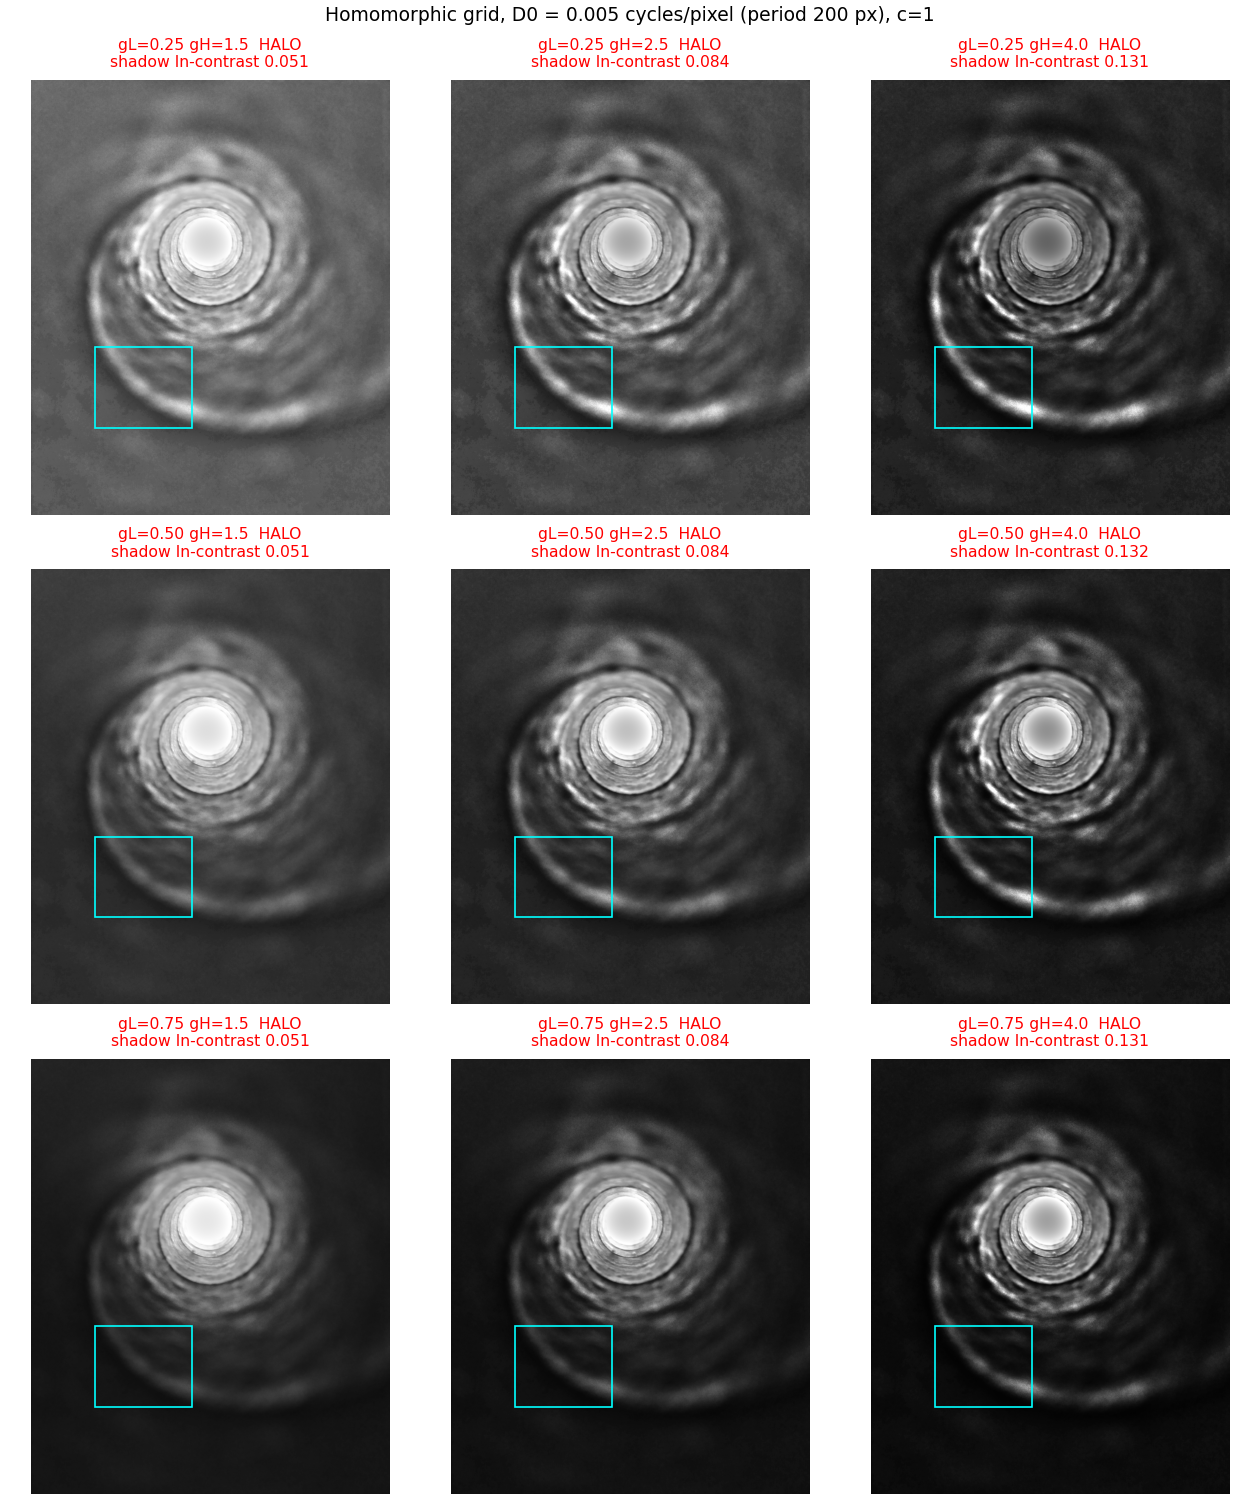
\includegraphics[width=0.62\linewidth]{q3_grid_D0_0p005}\par\vskip 3pt{\small\textbf{Figure 3.3.} Homomorphic grid, D0 = 0.005 cycles/pixel (rows gamma\_L = 0.25, 0.5, 0.75; columns gamma\_H = 1.5, 2.5, 4). Titles give the shadow-box log-contrast; HALO = flagged.\par}\end{figure}
\begin{figure}[H]\centering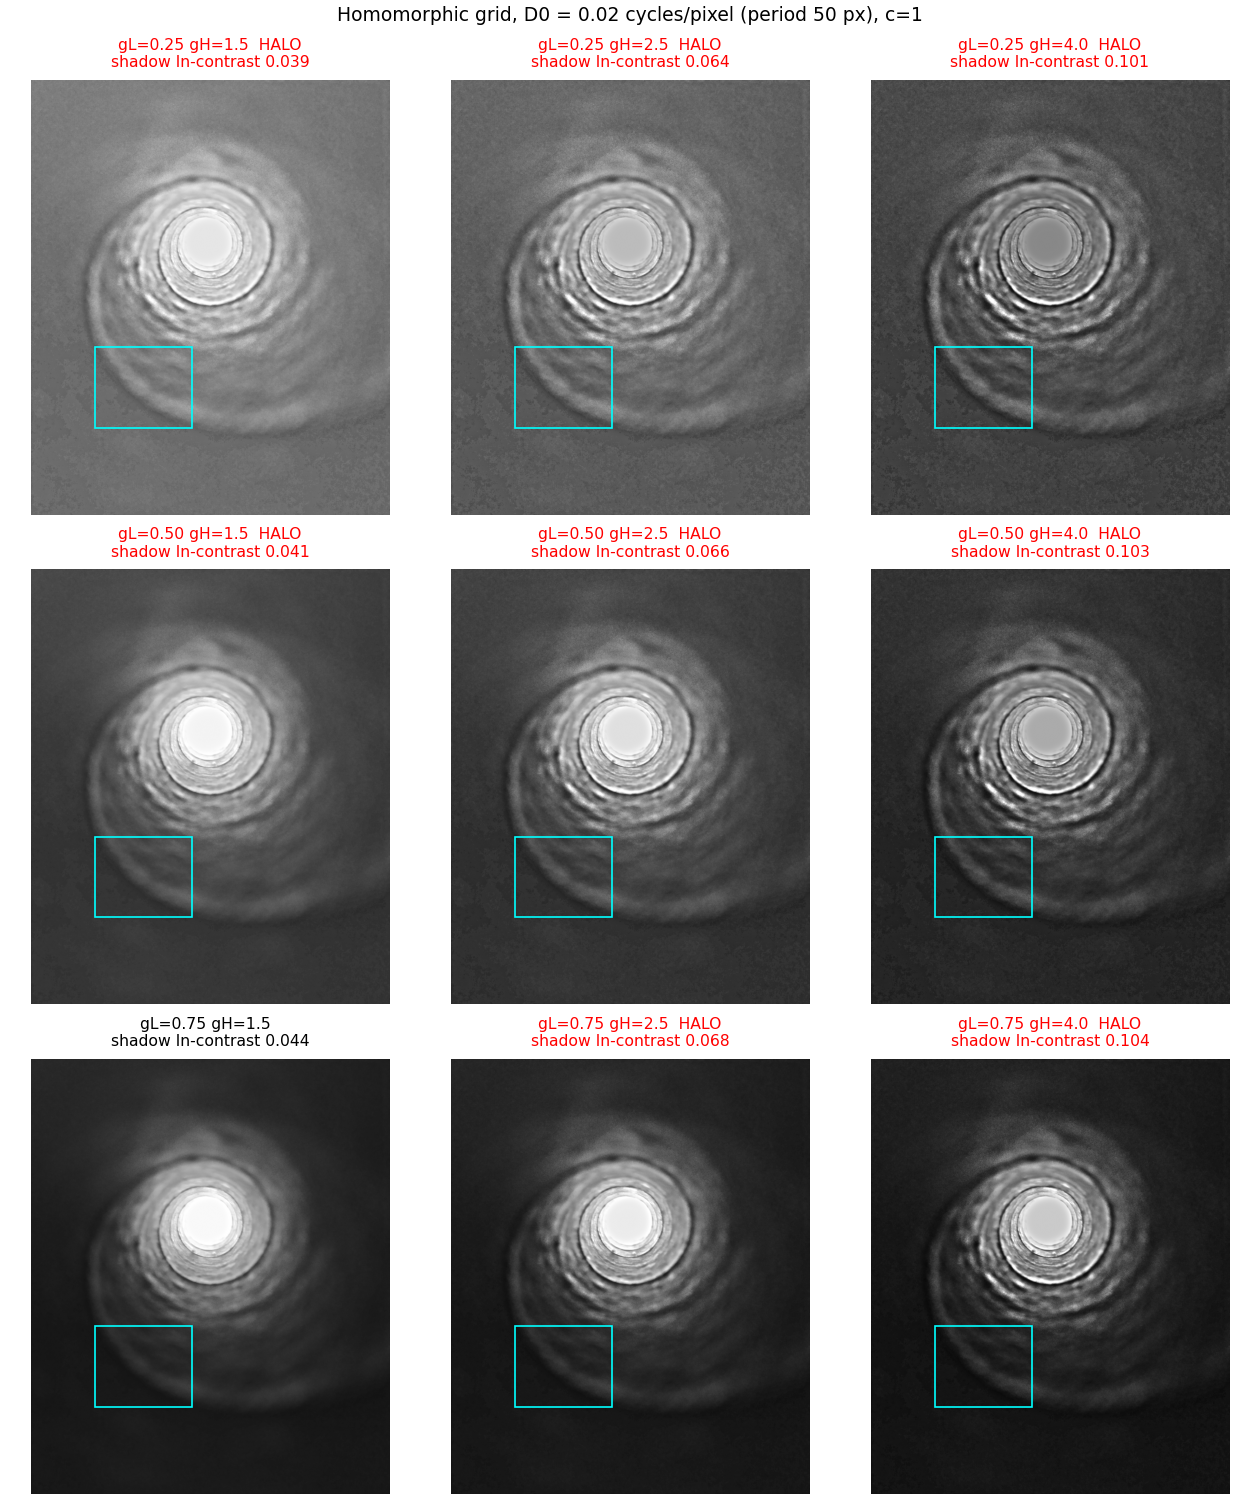
\includegraphics[width=0.62\linewidth]{q3_grid_D0_0p02}\par\vskip 3pt{\small\textbf{Figure 3.4.} Homomorphic grid, D0 = 0.02 cycles/pixel (rows gamma\_L = 0.25, 0.5, 0.75; columns gamma\_H = 1.5, 2.5, 4). Titles give the shadow-box log-contrast; HALO = flagged.\par}\end{figure}
\begin{figure}[H]\centering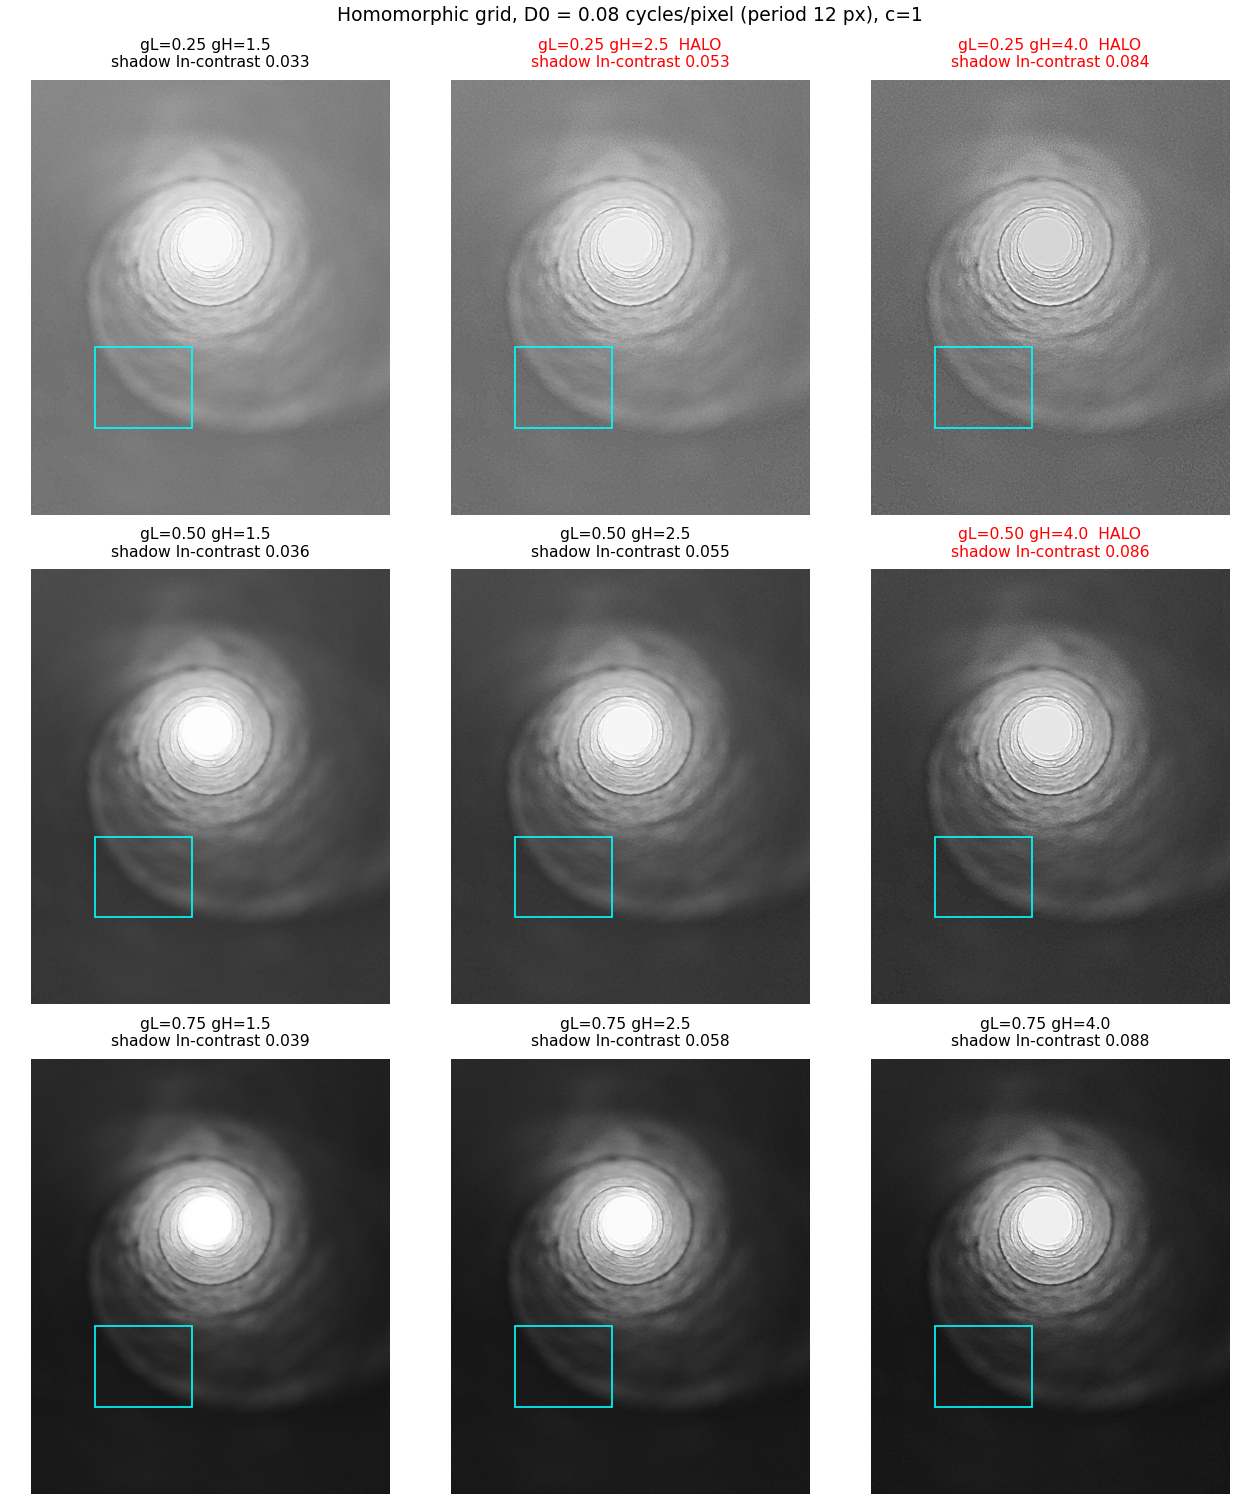
\includegraphics[width=0.62\linewidth]{q3_grid_D0_0p08}\par\vskip 3pt{\small\textbf{Figure 3.5.} Homomorphic grid, D0 = 0.08 cycles/pixel (rows gamma\_L = 0.25, 0.5, 0.75; columns gamma\_H = 1.5, 2.5, 4). Titles give the shadow-box log-contrast; HALO = flagged.\par}\end{figure}
\begin{table}[H]\centering\scriptsize{\small\textbf{Table 3.1.} Local contrast, flattening, saturation and halo measures. Shadow = faint tunnel wall box (rows 746-971, cols 180-450 of the 1214x1000 working image); corner = detail-free control box; ratio = shadow mean / aperture-disc mean; saturation = fraction of pixels \textgreater{}= 0.98 over the whole image; halo = rim overshoot / step S.\par}\vskip 3pt
\resizebox{\ifdim\width>\linewidth\linewidth\else\width\fi}{!}{\begin{tabular}{p{4.6cm}rrrrrrrrr}\toprule
\textbf{method} & \textbf{\begin{tabular}[b]{@{}c@{}}shadow mean\\{}level\end{tabular}} & \textbf{\begin{tabular}[b]{@{}c@{}}shadow local\\{}std (0-255)\end{tabular}} & \textbf{\begin{tabular}[b]{@{}c@{}}shadow std\\{}ln Y\end{tabular}} & \textbf{\begin{tabular}[b]{@{}c@{}}control std\\{}ln Y\end{tabular}} & \textbf{\begin{tabular}[b]{@{}c@{}}shadow/bright\\{}mean\end{tabular}} & \textbf{\begin{tabular}[b]{@{}c@{}}aperture\\{}mean level\end{tabular}} & \textbf{\begin{tabular}[b]{@{}c@{}}saturated \%\\{}(image)\end{tabular}} & \textbf{halo index} & \textbf{\begin{tabular}[b]{@{}c@{}}entropy\\{}(bits)\end{tabular}}\\\midrule
input (identity) & 18.7 & 0.71 & 0.0353 & 0.0259 & 0.0732 & 255.0 & 1.17 & 2.2e-17 & 5.75\\
global histogram equalisation & 105.8 & 7.50 & 0.157 & 0.0319 & 0.415 & 255.0 & 2.16 & 2.7e-16 & 5.44\\
homomorphic gL=0.5 gH=2.5 D0=0.08 (selected: halo-free, flattens) & 66.4 & 3.76 & 0.0553 & 0.0597 & 0.27 & 245.6 & 0.20 & 0.0497 & 6.52\\
homomorphic gL=0.75 gH=4 D0=0.08 & 33.8 & 3.10 & 0.0879 & 0.0954 & 0.142 & 238.8 & 0.15 & 0.0562 & 6.25\\
homomorphic gL=0.25 gH=4 D0=0.08 (strongest flattening, mild halo) & 111.2 & 9.51 & 0.0843 & 0.0948 & 0.52 & 213.8 & 0.13 & 0.253 & 6.52\\
homomorphic gL=0.5 gH=2.5 D0=0.02 (halo flagged) & 61.0 & 4.13 & 0.0659 & 0.0622 & 0.272 & 224.5 & 0.16 & 0.355 & 6.51\\
homomorphic gL=0.25 gH=4 D0=0.005 (strong halo) & 49.5 & 6.97 & 0.131 & 0.0989 & 0.409 & 121.0 & 0.11 & 3.76 & 6.25\\
\bottomrule\end{tabular}}\end{table}
\begin{figure}[H]\centering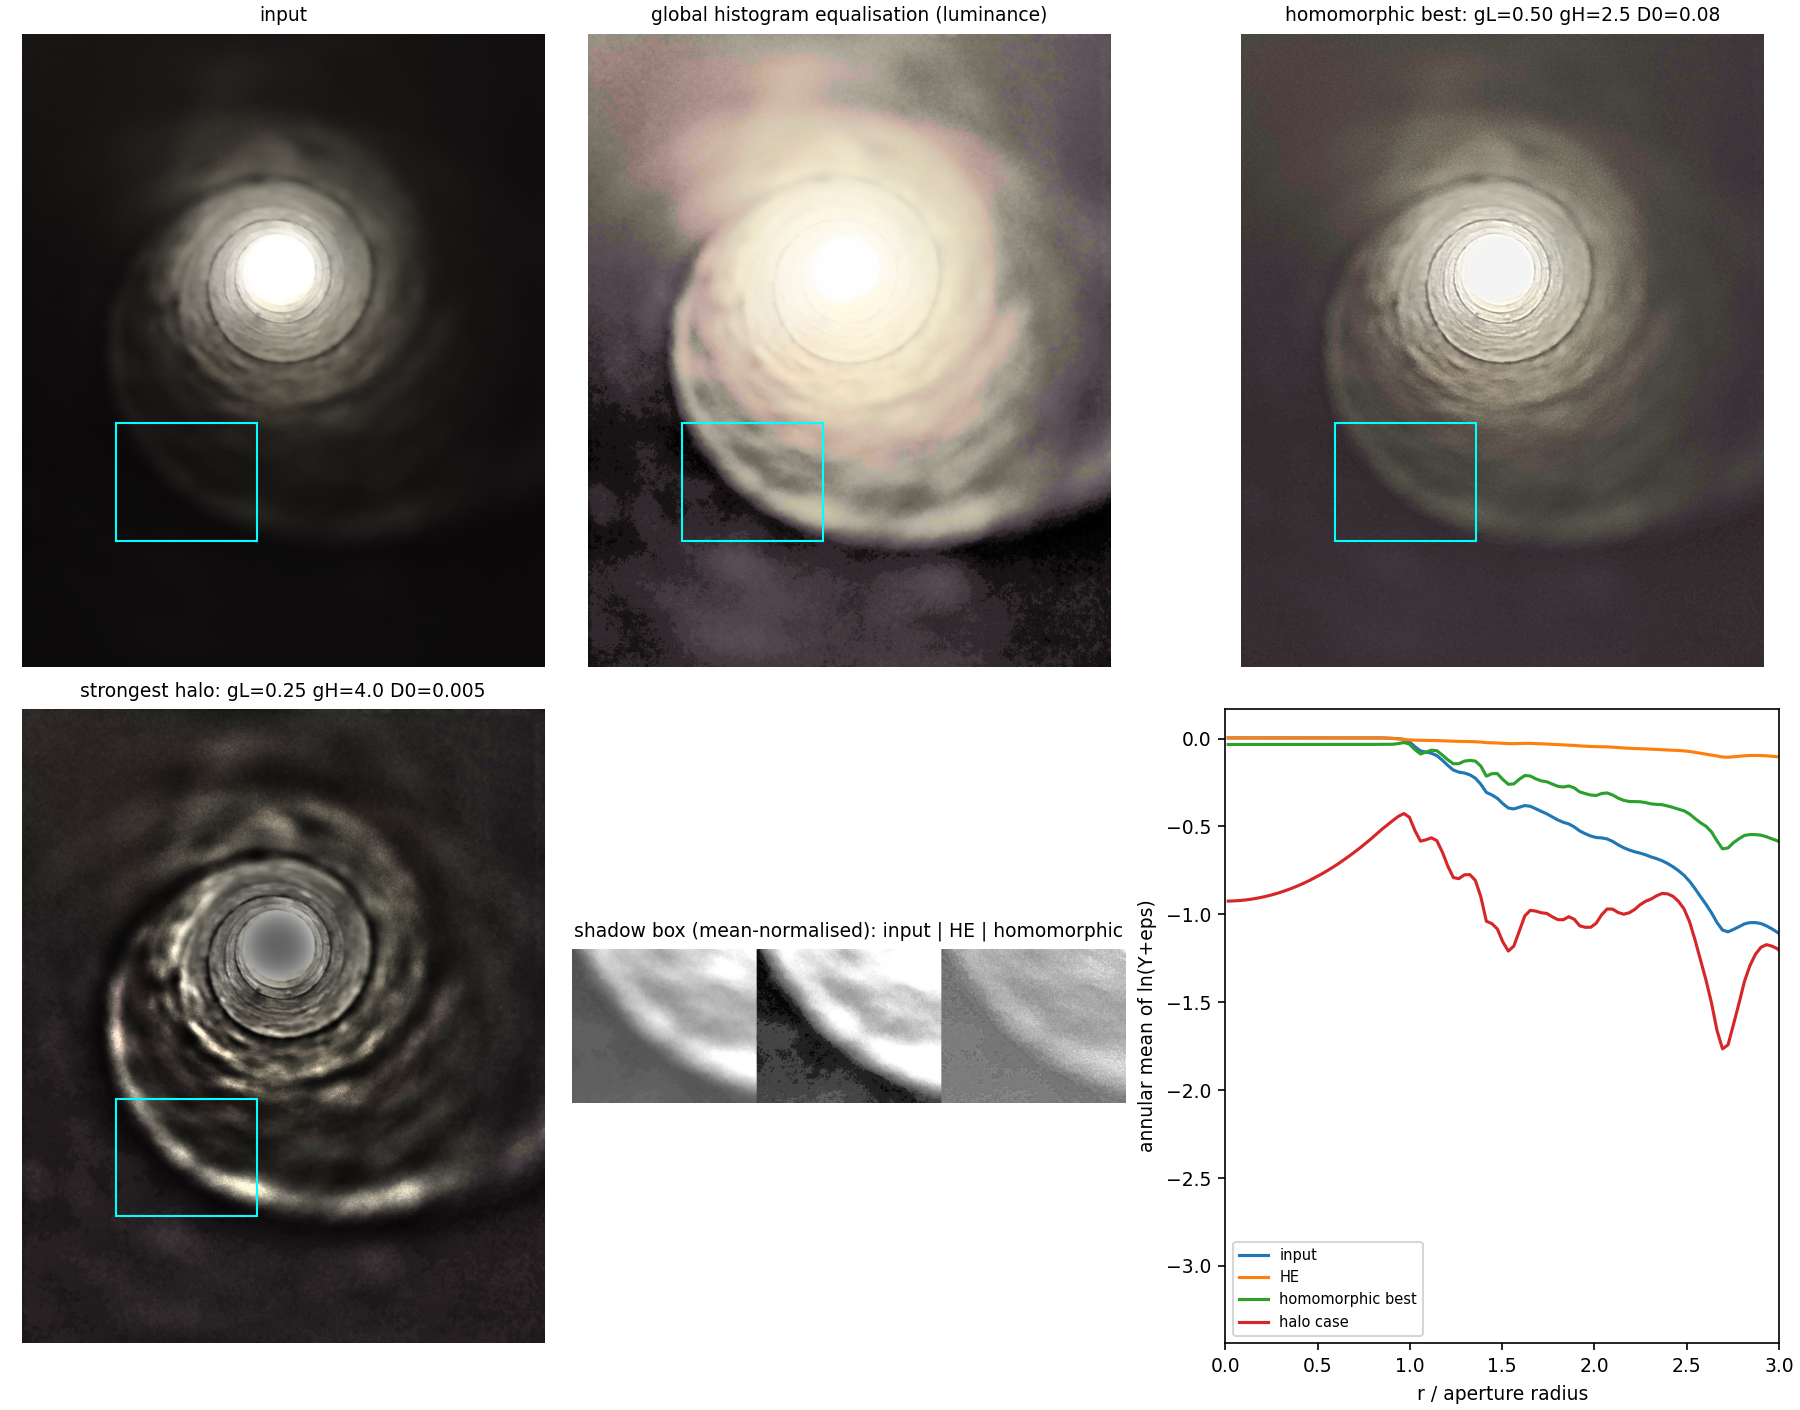
\includegraphics[width=1.00\linewidth]{q3_comparison}\par\vskip 3pt{\small\textbf{Figure 3.6.} Input, global histogram equalisation, the selected homomorphic setting and the strongest halo case; shadow-box crops (each normalised to the same mean so that contrast, not level, is compared) and annular log-profiles about the aperture centre (r in units of the aperture radius).\par}\end{figure}
\textbf{Settings that flatten illumination while preserving local contrast (no halo).} The DC gain $\gamma_L$ controls the compression of the illumination: shadow/bright ratio is 0.073 for the input and 0.142, 0.271, 0.52 for $\gamma_L=0.75,0.5,0.25$ (at $D_0=0.08$), while $\gamma_H$ sets the boost of detail (shadow log-contrast 0.0356 for $\gamma_H=1.5$ vs 0.0859 for $\gamma_H=4$ at $\gamma_L=0.5$). A large $D_0$ (0.08 cycles/pixel, i.e. detail finer than 12 px) keeps the high-boost band narrow and local; $\gamma_L=0.5$, $\gamma_H=2.5$, $D_0=0.08$ is selected by the explicit rule 'maximum shadow log-contrast among settings with no halo flag, \textless{}5\% saturated pixels and flattening ratio \textgreater{}= 0.25' (it lifts the shadow wall from mean level 18.7 to 66.4, reduces the shadow/bright ratio from 0.073 to 0.27, keeps the aperture below clipping with 0.20\% saturated pixels vs 1.17\% in the input, and has halo index 0.05). \textbf{Halo settings:} a small $D_0$ with large $\gamma_H$ and small $\gamma_L$ makes the filter boost a wide band around the strong aperture edge: the strongest case is $\gamma_L=0.25$, $\gamma_H=4.0$, $D_0=0.005$ (halo index 3.8): a bright rim ripples inside the aperture edge, the aperture interior is turned into a grey disc (its plateau is attenuated by the large step at the edge while the wall rings are over-emphasised), and the tunnel wall shows bright concentric 'glow' rims at 1.3-2.7 $R_e$ (Figure 3.6, bottom left; negative values of the outer undershoot index mean that the monotone fall-off outside the aperture is preserved in all cases).

\textbf{Comparison with plain global histogram equalisation (implemented from scratch: 8-bit luminance, cdf mapping, colour restored by the luminance ratio).} HE yields the largest \textit{raw} local contrast in the shadow box (mean local std 7.50 vs 3.76 for the selected homomorphic setting and 0.71 for the input; log-contrast 0.157 vs 0.0553 vs 0.0353). But (i) it lifts the \textit{entire} image (shadow mean level 106 vs 19 in the input), which turns the aperture surround into a washed-out, colour-cast glow (Figure 3.6); (ii) the bright aperture is left at 255 (100\% of the disc pixels are $\ge0.98$, as in the input) and the saturated fraction of the whole image doubles (2.16\% vs 1.17\%), i.e. HE blows out more of the bright region than it recovers; (iii) the HE mapping is global and applies the same stretch to noise: the detail-free control region has log-contrast 0.0319 (input 0.0259) - here HE is actually \textit{more noise-selective} than the homomorphic filter (control 0.0597), because the filter's high-frequency gain $\gamma_H$ boosts pixel noise and JPEG artefacts wherever the image is dark (the control ratio control/shadow is 0.20 for HE and 1.08 for the selected homomorphic setting; a value near 1 means the extra 'contrast' is mostly noise). (iv) HE has no parameter to trade flattening against halo, while the homomorphic filter cleanly separates the scale at which detail is boosted ($D_0$) from the strength of the compression ($\gamma_L$). A stronger homomorphic setting ($\gamma_L=0.25$, $\gamma_H=4$, $D_0=0.08$) exceeds HE in raw shadow contrast (9.51 vs 7.50), flattening (0.52 vs 0.41) and saturation (0.13\% vs 2.16\%) but is flagged for a mild halo (index 0.25) and amplifies the control region even more (0.0948).

\textbf{Verdict.} Neither method wins on every axis, and the numbers do not support a blanket claim that the homomorphic filter 'recovers more shadow detail': HE has the larger raw shadow contrast of the halo-free settings and the better detail-to-noise ratio. The homomorphic filter wins on \textit{not blowing out the bright region} (the aperture is pulled below clipping, the saturated fraction falls rather than doubles), on colour and tonal fidelity (no global wash-out; relative brightness of structures is preserved by construction), and on controllability; it loses on noise amplification in dark regions because the boost $\gamma_H$ is spatially uniform and the shadows are noisy. The reason is structural: the log makes the filter act on \textit{ratios}, so a given multiplicative detail is boosted equally in the shadow and in the lit regions, whereas HE redistributes grey levels according to the histogram (most pixels are dark, so HE assigns them most of the output range - good for shadow contrast, bad for the bright region, which has few pixels and gets squeezed into the top bins).

\section{Question 4 - Edge-preserving smoothing: bilateral vs Kuwahara}
\textbf{Data.} The provided clean ground truth (512x512, 41 grey levels: flat regions at 20/60/200, a horizontal ramp rectangle 66-103, and a disc of radius 104.0 px) is corrupted with zero-mean Gaussian noise of \textbf{standard deviation }$\sigma=15$ (8-bit levels; seed 2026; noisy input PSNR 24.70 dB, SSIM 0.257; the Immerkaer estimate of the noise level from the noisy image alone is 14.99). The noisy input is not clipped before filtering. PSNR (data range 255) and SSIM (Gaussian window, Section 0) are computed against the clean image with the filter output clipped to [0,255].

\subsection{4.1 Implementation and matched-strength comparison}
\textbf{Bilateral filter} (from scratch, shifted-slice sums, reflect boundary, window radius $\min(\lceil3\sigma_s\rceil,12)$): 

\begin{equation}\hat I(p)=\frac{\sum_{q}w_s(\|p-q\|)\,w_r(I_q-I_p)\,I_q}{\sum_{q}w_s(\|p-q\|)\,w_r(I_q-I_p)},\quad w_s=e^{-\|p-q\|^2/(2\sigma_s^2)},\ w_r=e^{-(I_q-I_p)^2/(2\sigma_r^2)}\end{equation}
\textbf{Classical Kuwahara filter} (from scratch with integral images): for an $N\times N$ window ($N$ odd, $k=(N-1)/2$, $m=k+1$) the four overlapping $m\times m$ sub-windows (top-left, top-right, bottom-left, bottom-right) share the centre row and column; the output is the mean of the sub-window with the smallest (population) variance. Both are verified against brute-force single-pixel evaluations, constant images, exactly preserved noise-free steps, and limiting cases (tests/test\_q4.py).

\subsubsection{4.1a Matched effective smoothing strength}
\textbf{Definition.} The effective smoothing strength of a filter $F$ is its \textit{noise-variance reduction factor on a flat region}, $S(F)=\mathrm{Var}[F(n)]/\mathrm{Var}[n]$ for a zero-mean white-noise field $n$ (measured on a 176x176 field of $\sigma=15$ noise, interior only), i.e. the reciprocal of the effective number of averaged independent samples. Two filters are \textbf{matched} when $S(F_1)=S(F_2)$. Justification: in flat regions an edge-preserving filter must behave as an averaging filter, so the number of samples it averages (the 'effective spatial footprint') sets how much noise it removes; an edge-aware term then only changes behaviour near edges, which is exactly what the comparison should isolate. For Kuwahara with sub-window size $m$ the selected window is a mean of $m^2$ samples and $S\approx1/m^2$ (because for Gaussian data a window's mean is independent of its variance, selecting by variance does not bias the mean); a Gaussian kernel of width $\sigma_s$ averages $n_{eff}=(\sum w)^2/\sum w^2\approx4\pi\sigma_s^2$ samples, giving the analytic pairing $\sigma_s=m/(2\sqrt\pi)$. Because the range term makes the bilateral kernel narrower than the Gaussian in the presence of noise, the analytic pairing under-smooths; $\sigma_s$ is therefore found numerically by bisection so that the measured bilateral $S$ equals the measured Kuwahara $S$ (with $\sigma_r=2\sigma$, the rule discussed in 4.3).

\begin{table}[H]\centering\scriptsize{\small\textbf{Table 4.1.} Matching table (sigma=15 flat noise field, sigma\_r = 2 sigma). S = noise variance ratio. 'analytic sigma\_s' = m/(2 sqrt(pi)) from n\_eff = m\textasciicircum{}2; 'matched sigma\_s' from bisection on the measured S. 'reached' = matched S within 5\% of the Kuwahara S (limited by the largest allowed window 25x25).\par}\vskip 3pt
\resizebox{\ifdim\width>\linewidth\linewidth\else\width\fi}{!}{\begin{tabular}{rrrrrrrrrrr}\toprule
\textbf{N} & \textbf{m} & \textbf{\begin{tabular}[b]{@{}c@{}}S Kuwahara\\{}(measured)\end{tabular}} & \textbf{1/m\textasciicircum{}2} & \textbf{\begin{tabular}[b]{@{}c@{}}S\\{}soft-Kuwahara\end{tabular}} & \textbf{\begin{tabular}[b]{@{}c@{}}analytic\\{}sigma\_s\end{tabular}} & \textbf{\begin{tabular}[b]{@{}c@{}}S bilateral\\{}at analytic\\{}sigma\_s\end{tabular}} & \textbf{\begin{tabular}[b]{@{}c@{}}matched\\{}sigma\_s\end{tabular}} & \textbf{\begin{tabular}[b]{@{}c@{}}S bilateral\\{}at matched\end{tabular}} & \textbf{reached} & \textbf{\begin{tabular}[b]{@{}c@{}}bilateral\\{}window\end{tabular}}\\\midrule
5 & 3 & 0.1205 & 0.1111 & 0.05225 & 0.846 & 0.2264 & 1.271 & 0.1205 & yes & 9\\
7 & 4 & 0.06563 & 0.0625 & 0.02474 & 1.128 & 0.1429 & 2.215 & 0.06563 & yes & 15\\
9 & 5 & 0.04129 & 0.04 & 0.01405 & 1.410 & 0.1049 & 5.999 & 0.04352 & NO & 25\\
11 & 6 & 0.02759 & 0.02778 & 0.008916 & 1.693 & 0.08457 & 5.999 & 0.04352 & NO & 25\\
15 & 8 & 0.01508 & 0.01562 & 0.004475 & 2.257 & 0.06467 & 5.999 & 0.04352 & NO & 25\\
\bottomrule\end{tabular}}\end{table}
\subsubsection{4.1b PSNR/SSIM evaluation and crops}
\begin{table}[H]\centering\scriptsize{\small\textbf{Table 4.2.} Matched-strength comparison at sigma=15 (noisy input PSNR 24.70 dB / SSIM 0.257). Bilateral: sigma\_r = 2 sigma = 30 (rule-based, not tuned), sigma\_s from Table 4.1. Soft-Kuwahara (Section 4.2) uses tau = (Immerkaer sigma-hat)\textasciicircum{}2. Data range 255.\par}\vskip 3pt
\resizebox{\ifdim\width>\linewidth\linewidth\else\width\fi}{!}{\begin{tabular}{rrrrrrrr}\toprule
\textbf{N} & \textbf{\begin{tabular}[b]{@{}c@{}}bilateral\\{}sigma\_s\end{tabular}} & \textbf{\begin{tabular}[b]{@{}c@{}}bilateral\\{}PSNR\end{tabular}} & \textbf{\begin{tabular}[b]{@{}c@{}}bilateral\\{}SSIM\end{tabular}} & \textbf{\begin{tabular}[b]{@{}c@{}}Kuwahara\\{}PSNR\end{tabular}} & \textbf{\begin{tabular}[b]{@{}c@{}}Kuwahara\\{}SSIM\end{tabular}} & \textbf{soft PSNR} & \textbf{soft SSIM}\\\midrule
5 & 1.271 & 33.57 & 0.7473 & 33.53 & 0.7548 & 36.94 & 0.8910\\
7 & 2.215 & 35.98 & 0.8412 & 36.05 & 0.8565 & 39.61 & 0.9523\\
9 & 5.999 & 37.04 & 0.8661 & 37.86 & 0.9069 & 41.15 & 0.9734\\
11 & 5.999 & 37.04 & 0.8661 & 39.16 & 0.9348 & 41.93 & 0.9815\\
15 & 5.999 & 37.04 & 0.8661 & 40.71 & 0.9620 & 42.20 & 0.9864\\
\bottomrule\end{tabular}}\end{table}
\begin{table}[H]\centering\scriptsize{\small\textbf{Table 4.3.} Noise-level sweep at N=7 (sigma\_s matched to Kuwahara N=7 at each sigma, sigma\_r = 2 sigma).\par}\vskip 3pt
\resizebox{\ifdim\width>\linewidth\linewidth\else\width\fi}{!}{\begin{tabular}{rrrrrrrr}\toprule
\textbf{sigma} & \textbf{noisy PSNR} & \textbf{\begin{tabular}[b]{@{}c@{}}bilateral\\{}PSNR\end{tabular}} & \textbf{\begin{tabular}[b]{@{}c@{}}bilateral\\{}SSIM\end{tabular}} & \textbf{\begin{tabular}[b]{@{}c@{}}Kuwahara\\{}PSNR\end{tabular}} & \textbf{\begin{tabular}[b]{@{}c@{}}Kuwahara\\{}SSIM\end{tabular}} & \textbf{soft PSNR} & \textbf{soft SSIM}\\\midrule
10.0 & 28.15 & 39.48 & 0.9203 & 39.64 & 0.9295 & 43.09 & 0.9781\\
15.0 & 24.69 & 35.98 & 0.8401 & 36.04 & 0.8567 & 39.63 & 0.9527\\
20.0 & 22.26 & 33.49 & 0.7522 & 33.56 & 0.7757 & 37.28 & 0.9207\\
30.0 & 18.95 & 29.86 & 0.5854 & 30.12 & 0.6195 & 33.92 & 0.8435\\
\bottomrule\end{tabular}}\end{table}
\begin{table}[H]\centering\small{\small\textbf{Table 4.4.} Oracle view: bilateral PSNR/SSIM as sigma\_r varies (sigma\_s fixed at the matched value from Table 4.1; the clean image is used to read this table, so the best row is an oracle-tuned result, not a blind one).\par}\vskip 3pt
\resizebox{\ifdim\width>\linewidth\linewidth\else\width\fi}{!}{\begin{tabular}{rrrr}\toprule
\textbf{N} & \textbf{sigma\_r/sigma} & \textbf{PSNR} & \textbf{SSIM}\\\midrule
7 & 1.0 & 29.66 & 0.5192\\
7 & 2.0 & 35.98 & 0.8412\\
7 & 3.0 & 38.64 & 0.9334\\
7 & 4.0 & 38.94 & 0.9569\\
7 & 6.0 & 36.78 & 0.9643\\
11 & 1.0 & 30.32 & 0.5422\\
11 & 2.0 & 37.04 & 0.8661\\
11 & 3.0 & 39.27 & 0.9519\\
11 & 4.0 & 38.25 & 0.9700\\
11 & 6.0 & 33.93 & 0.9682\\
\bottomrule\end{tabular}}\end{table}
\begin{figure}[H]\centering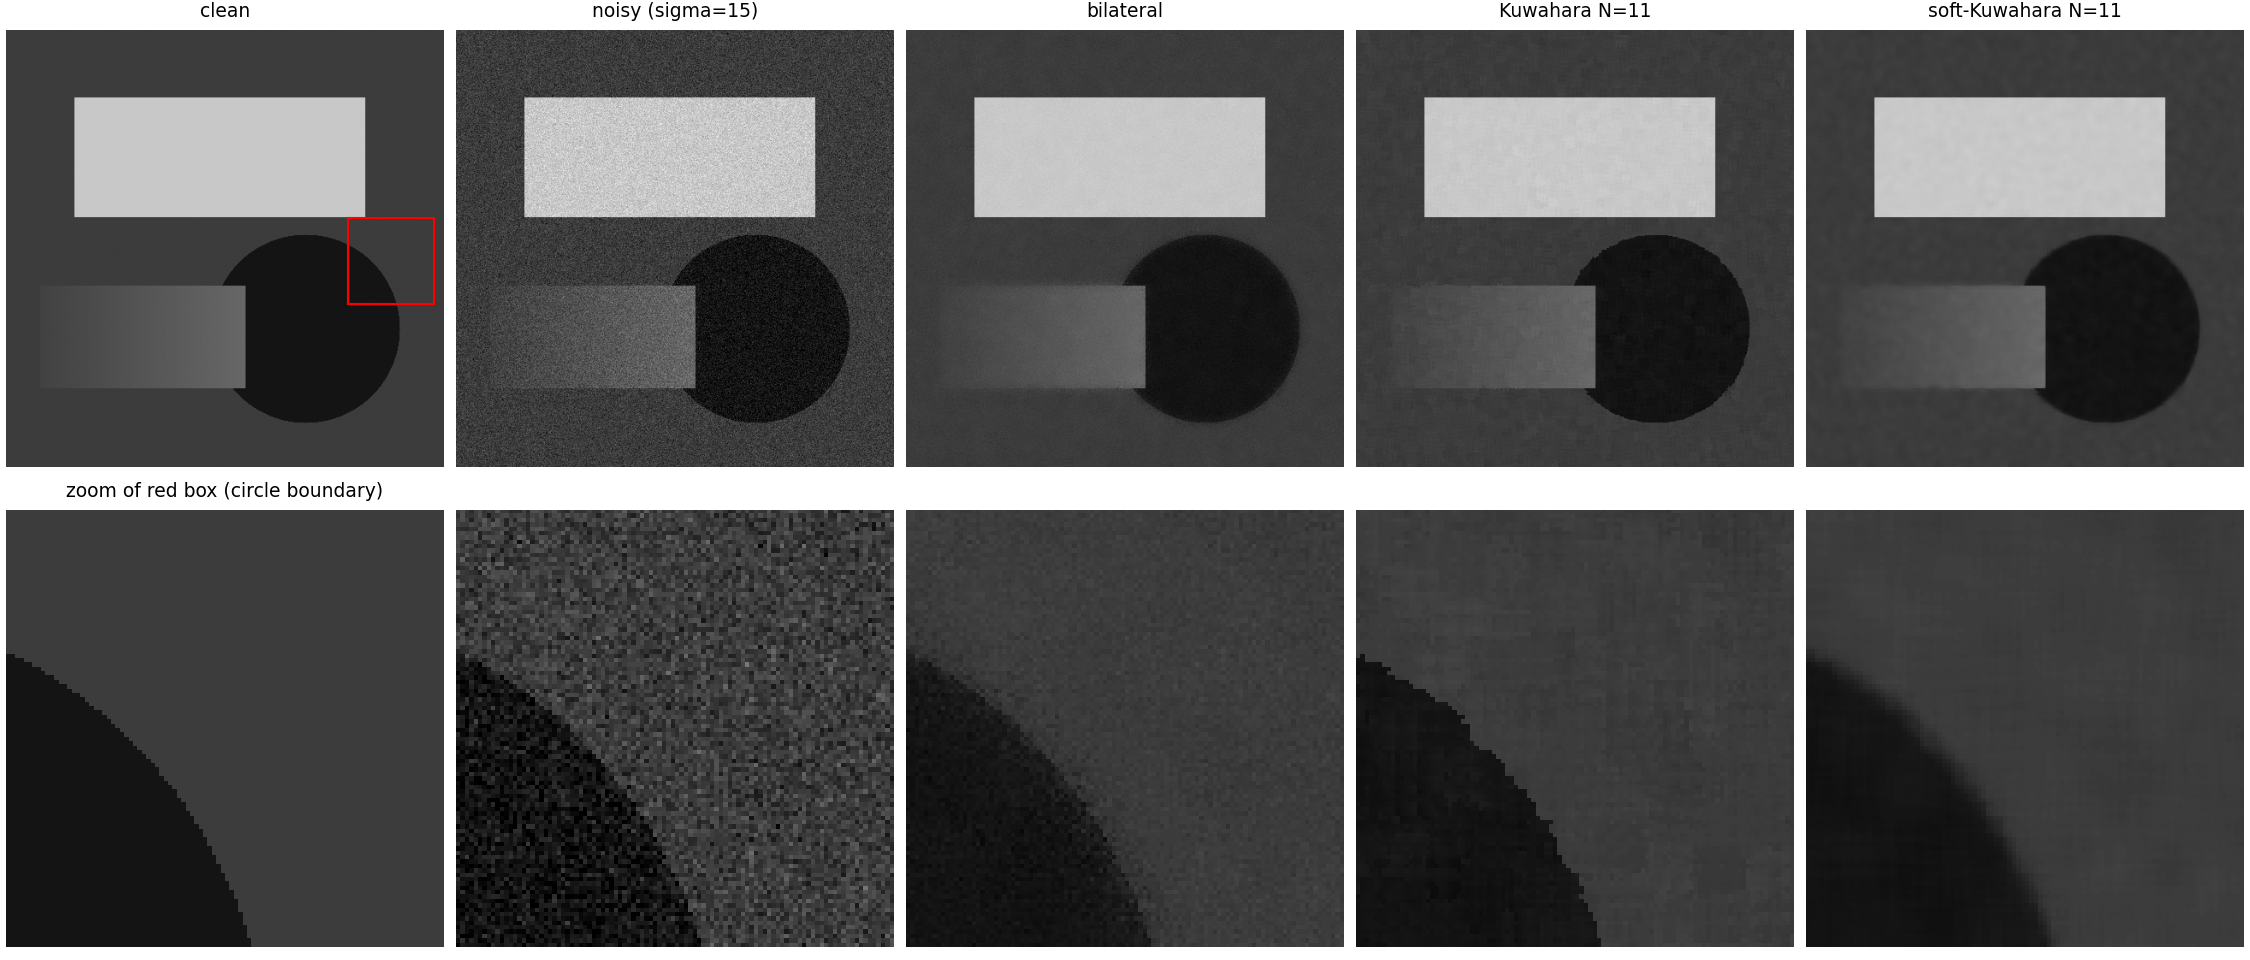
\includegraphics[width=1.00\linewidth]{q4_matched_outputs}\par\vskip 3pt{\small\textbf{Figure 4.1.} Matched-strength outputs at N=11 (bilateral sigma\_s from Table 4.1, sigma\_r=2 sigma, classical Kuwahara, soft-Kuwahara) with zoomed crops of the circle boundary (red box).\par}\end{figure}
\begin{figure}[H]\centering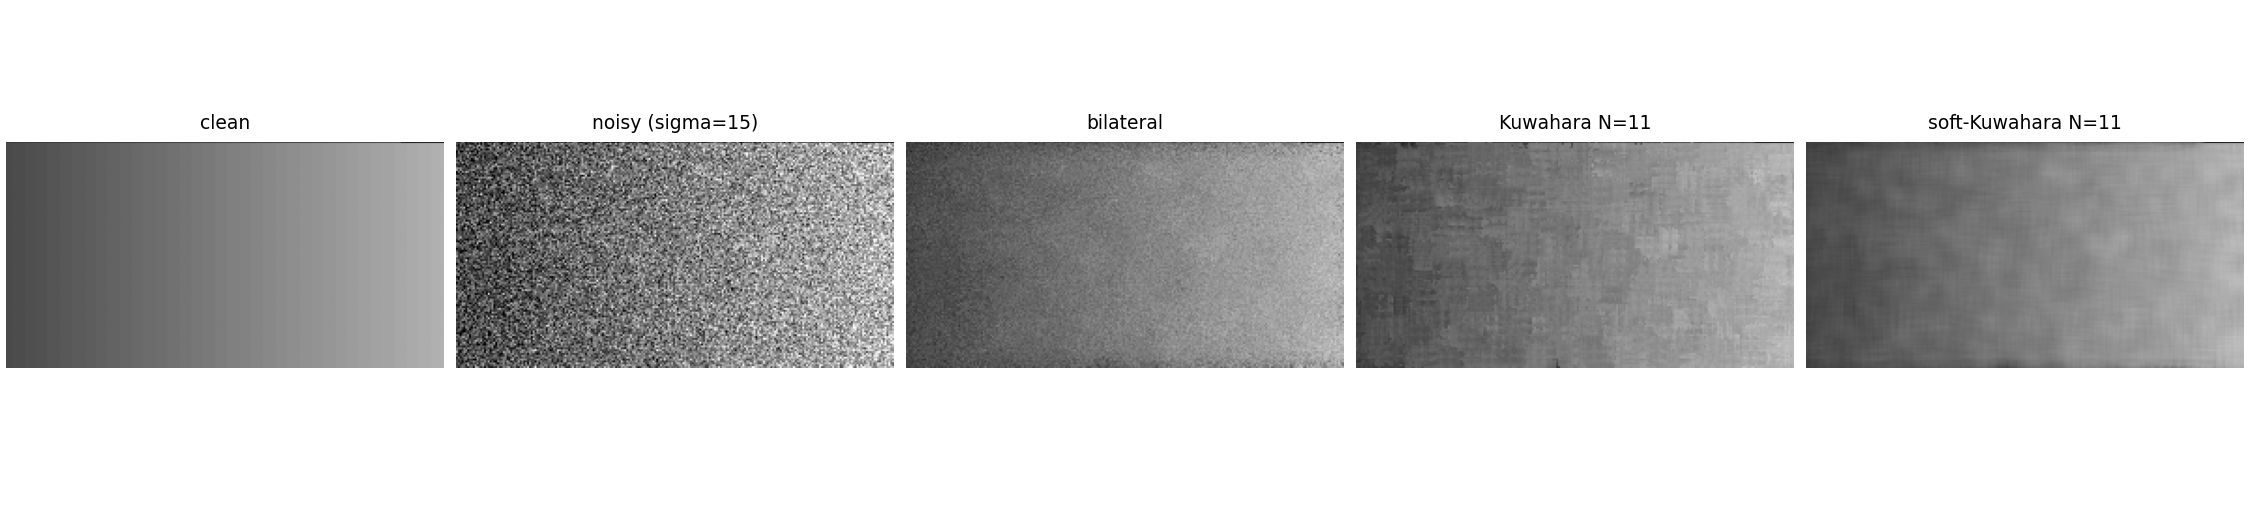
\includegraphics[width=1.00\linewidth]{q4_ramp_zoom}\par\vskip 3pt{\small\textbf{Figure 4.2.} The ramp rectangle (noisy input, N = 11, display range 40-130): the classical Kuwahara output breaks the smooth ramp into patches of roughly the sub-window size with abrupt boundaries (blockiness); the bilateral output keeps residual grain but no patches; the soft-Kuwahara output is smooth.\par}\end{figure}
\textbf{Reading Tables 4.1-4.4 and Figures 4.1-4.2.} (1) \textit{Where the strengths are matched} (N = 5 and 7; N = 9 is within 5.3\% of the target) the classical Kuwahara filter and the rule-based bilateral filter (sigma\_r = 2 sigma) are practically equal in PSNR: 33.57 vs 33.53 dB (N=5) and 35.98 vs 36.05 dB (N=7), with a small SSIM advantage for Kuwahara (0.755 vs 0.747 and 0.857 vs 0.841); the noise sweep of Table 4.3 shows the same picture from sigma = 10 to 30 (differences of 0.06-0.26 dB in favour of Kuwahara, 0.01-0.03 in SSIM). (2) \textit{For N \textgreater{}= 11 the strength match is not reachable}: the bilateral filter with sigma\_r = 2 sigma reduces the flat-field variance only to 0.0435 even with its largest allowed window (25x25), against 0.0276 (N=11) and 0.0151 (N=15) for Kuwahara, so the bilateral outputs for N = 9, 11, 15 are identical (37.04 dB) and the larger Kuwahara PSNR there (39.16 and 40.71 dB) partly reflects stronger smoothing, not better edge preservation: those rows are \textit{not} matched comparisons. (3) \textit{The parameter sigma\_r matters more than the matching:} with the clean image used to pick sigma\_r (Table 4.4, oracle) the bilateral filter reaches 38.94 dB / SSIM 0.957 at N = 7 (sigma\_r = 4 sigma) - 3.0 dB above its rule-based value - and 39.27 dB / 0.952 at N = 11 (sigma\_r = 3 sigma), i.e. equal to classical Kuwahara at N = 11 (39.16 dB / 0.935). (4) \textit{Edge behaviour} (Figure 4.1, zoom on the disc boundary, \textbar{}Delta I\textbar{} = 40 so NCR = 0.375, close to the breakdown region of Section 4.3): the bilateral output has a visibly softened edge and residual grain along it; classical Kuwahara keeps the edge sharp but with jagged, block-shaped steps; soft-Kuwahara gives a smooth, slightly blurred boundary and the cleanest flat areas. (5) The soft-Kuwahara has the highest PSNR/SSIM at every N (36.9 to 42.2 dB), but its flat-field variance ratio is 2.3-3.4 times lower than that of the classical filter at the same N (Table 4.1), so part of the gain is stronger smoothing; compared at a similar flat-field strength (soft N = 5, ratio 0.0522, against classical N = 7, ratio 0.0656) it is still 0.9 dB better.

\subsection{4.2 Kuwahara blockiness and complexity}
\subsubsection{4.2a Why the hard arg-min causes blockiness}
The classical output at pixel $p$ is $\hat I(p)=\mu_{i^*(p)}(p)$ with $i^*(p)=\arg\min_i\sigma^2_i(p)$: a \textit{discontinuous} function of the data. In any region without a sharp edge (a smooth ramp, a curved boundary, texture) the four sub-window variances are nearly equal and differ only by noise or by tiny differences in curvature; which window wins is then decided by arbitrary small fluctuations, and it changes abruptly between neighbouring pixels. Because the winning window is an $m\times m$ box whose mean is \textit{constant} over a region shifted by $\pm k$ pixels, the output is piecewise constant with patches of the size of the sub-window ($m=(N+1)/2$: 6x6 for $N=11$, 8x8 for $N=15$) and straight, axis-aligned jumps between patches: staircase edges on curved boundaries, plateaus on ramps. It is not blur (a selected window mean is not a smoothing of the transition: a clean step is reproduced exactly, tested), not ringing (a mean of a window never leaves the range of the window's data, so there is no overshoot): it is a \textit{selection discontinuity} (a hard decision, a non-Lipschitz map from data to output) whose spatial scale grows with $N$. Figure 4.3 shows the selection map (window index) next to the output: in the flat regions the winning window changes in irregular blobs of roughly the sub-window size (the winner is decided by noise), along the disc boundary it forms a coherent band, and the patch boundaries of the classical output (visible as steps on the boundary and as patches on the ramp, Figures 4.2 and 4.4) lie where the index jumps.

\begin{figure}[H]\centering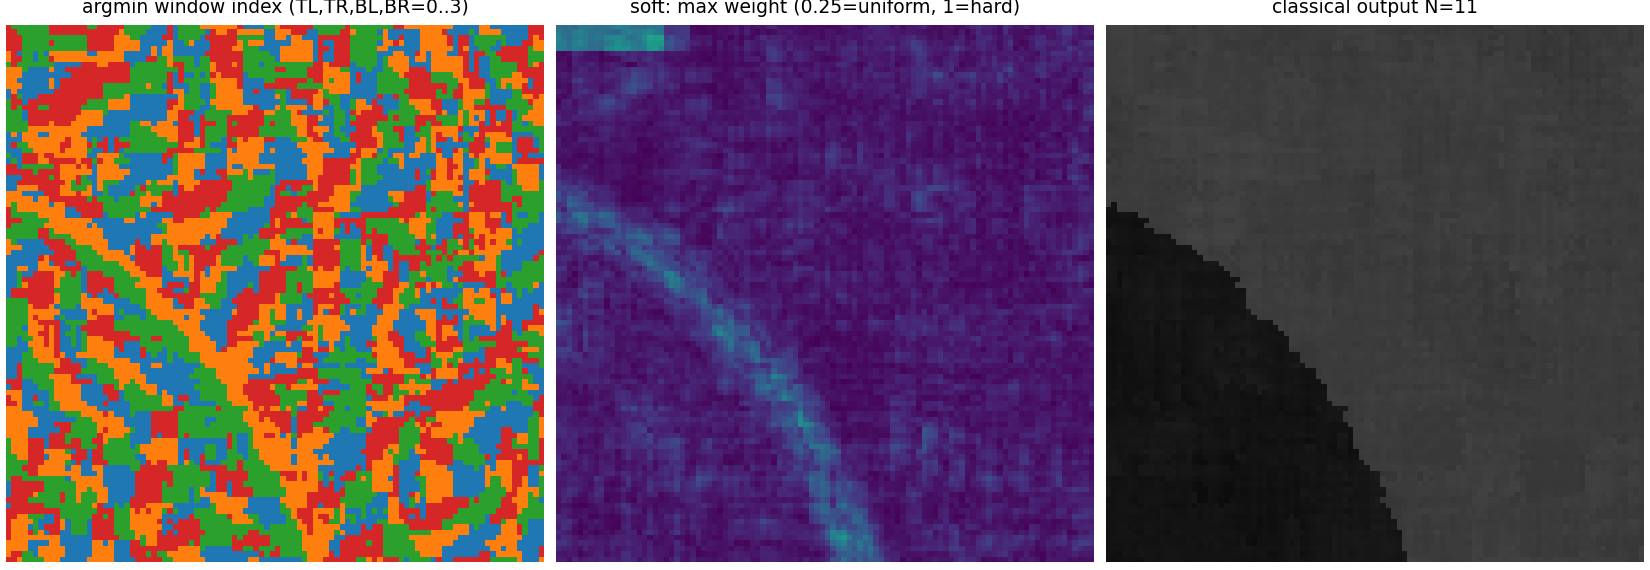
\includegraphics[width=1.00\linewidth]{q4_selection_map}\par\vskip 3pt{\small\textbf{Figure 4.3.} Left: index of the arg-min window (0..3 = TL, TR, BL, BR) over the circle-boundary crop (N = 11, noisy input): the winner flips in blobs. Middle: maximum softmax weight of the soft-Kuwahara (0.25 = uniform, 1 = hard selection). Right: the classical output.\par}\end{figure}
\subsubsection{4.2b De-blocking: Soft-Kuwahara}
\textbf{Modification.} Replace the arg-min by a softmax over the four sub-window variances,

\begin{equation}\hat I(p)=\frac{\sum_{i=1}^{4}w_i\,\mu_i}{\sum_{i=1}^{4}w_i},\qquad w_i=\exp\!\Big(-\frac{\sigma_i^2-\min_j\sigma_j^2}{\tau}\Big),\qquad \tau=\hat\sigma_{n}^{2}\end{equation}
with $\hat\sigma_n$ the Immerkaer estimate of the noise from the noisy image ($\tau\to0$ gives the classical filter, $\tau\to\infty$ the average of the four window means; both limits are tested). The sample variance of an $m^2$-sample flat window fluctuates by $\sigma^2\sqrt{2/(m^2-1)}$ around $\sigma^2$, so with $\tau=\hat\sigma^2$ the windows are weighted nearly equally in flat regions (no arbitrary winner) while at a strong edge the variance difference ($\approx\Delta I^2/4$) is much larger than $\tau$ and the weights become one-hot (edge kept). At the low-contrast disc boundary of the test image ($|\Delta I|=40$, $\sigma=15$) the difference ($\approx400$) is comparable to $\tau\approx225$, so the weights are only partly concentrated (maximum weight 0.5-0.6 along the boundary, Figure 4.3 middle, against 0.25-0.3 in flat areas): this is the regime in which the soft filter smooths the boundary slightly. This continuous weighting makes the output a smooth function of the data.

\textbf{Metrics for blockiness} (explicit; computed on the noisy input at $\sigma=15$, averaged over 4 independent noise realisations, and on the \textit{noise-free} image, where every non-zero value is pure filter artefact): (i) \textit{TV excess}: mean absolute gradient (anisotropic total variation per pixel) of the output minus that of the clean image, on pixels farther than 8 px from any strong edge, so that true edges are excluded - plateau-and-jump structure raises TV; (ii) \textit{ramp gradient irregularity}: standard deviation of the horizontal pixel difference over the ramp rectangle, whose clean value is a constant slope (a blocky output has plateaus of zero gradient separated by jumps, so this standard deviation grows: this is the boundary-gradient-discontinuity measure suggested in the assignment); (iii) \textit{ramp RMS deviation} from the clean ramp (grey levels); (iv) \textit{circle contour deviation}: RMS (px) of the difference between the sub-pixel contour radius $r(\theta)$ of the output and that of the clean image (same ray-casting procedure on both, 720 rays; rays on which the disc is hidden by the ramp rectangle are excluded), which is sensitive to staircase displacement of the boundary. Table 4.5 lists them; Figure 4.4 shows before/after crops at identical window sizes.

\begin{table}[H]\centering\scriptsize{\small\textbf{Table 4.5.} Blockiness metrics. Left block: noisy input (sigma = 15, mean of 4 noise draws); right block: noise-free input (pure artefact of the filter). TV excess = mean \textbar{}gradient\textbar{} in smooth regions minus that of the clean image; ramp gradient std = std of the horizontal difference over the ramp (clean image: the quantisation of the 41-level ramp, value in the last rows); ramp RMS dev = grey levels; contour dev = px.\par}\vskip 3pt
\resizebox{\ifdim\width>\linewidth\linewidth\else\width\fi}{!}{\begin{tabular}{rlrrrrrrrr}\toprule
\textbf{N} & \textbf{filter} & \textbf{\begin{tabular}[b]{@{}c@{}}TV excess\\{}(noisy)\end{tabular}} & \textbf{\begin{tabular}[b]{@{}c@{}}ramp grad\\{}std (noisy)\end{tabular}} & \textbf{\begin{tabular}[b]{@{}c@{}}ramp RMS dev\\{}(noisy)\end{tabular}} & \textbf{\begin{tabular}[b]{@{}c@{}}contour dev\\{}px (noisy)\end{tabular}} & \textbf{\begin{tabular}[b]{@{}c@{}}TV excess\\{}(clean in)\end{tabular}} & \textbf{\begin{tabular}[b]{@{}c@{}}ramp grad\\{}std (clean\\{}in)\end{tabular}} & \textbf{\begin{tabular}[b]{@{}c@{}}ramp RMS dev\\{}(clean in)\end{tabular}} & \textbf{\begin{tabular}[b]{@{}c@{}}contour dev\\{}px (clean\\{}in)\end{tabular}}\\\midrule
7 & classical & 2.84 & 3.885 & 3.89 & 0.43 & 1.3e-04 & 0.363 & 0.00 & 0.060\\
7 & soft & 1.25 & 1.614 & 2.45 & 0.29 & 4.4e-05 & 0.054 & 0.26 & 0.123\\
7 & bilateral & 3.52 & 4.631 & 3.90 & 0.27 & 8.7e-05 & 0.025 & 0.27 & 0.044\\
11 & classical & 1.64 & 2.328 & 2.59 & 0.56 & 0.00992 & 0.453 & 0.19 & 0.062\\
11 & soft & 0.637 & 0.815 & 1.53 & 0.34 & 3.0e-04 & 0.027 & 0.29 & 0.149\\
11 & bilateral & 3.39 & 4.327 & 3.18 & 0.60 & 0.00536 & 0.009 & 0.36 & 0.029\\
15 & classical & 1.11 & 1.675 & 1.99 & 0.70 & 0.0131 & 0.587 & 0.60 & 0.062\\
15 & soft & 0.4 & 0.518 & 1.09 & 0.54 & 0.0015 & 0.047 & 0.25 & 0.402\\
15 & bilateral & 3.39 & 4.327 & 3.18 & 0.60 & 0.00536 & 0.009 & 0.36 & 0.029\\
- & clean image itself & 0 & 0.363 & 0 & 0 & 0 & 0.363 & 0 & 0\\
\bottomrule\end{tabular}}\end{table}
\begin{figure}[H]\centering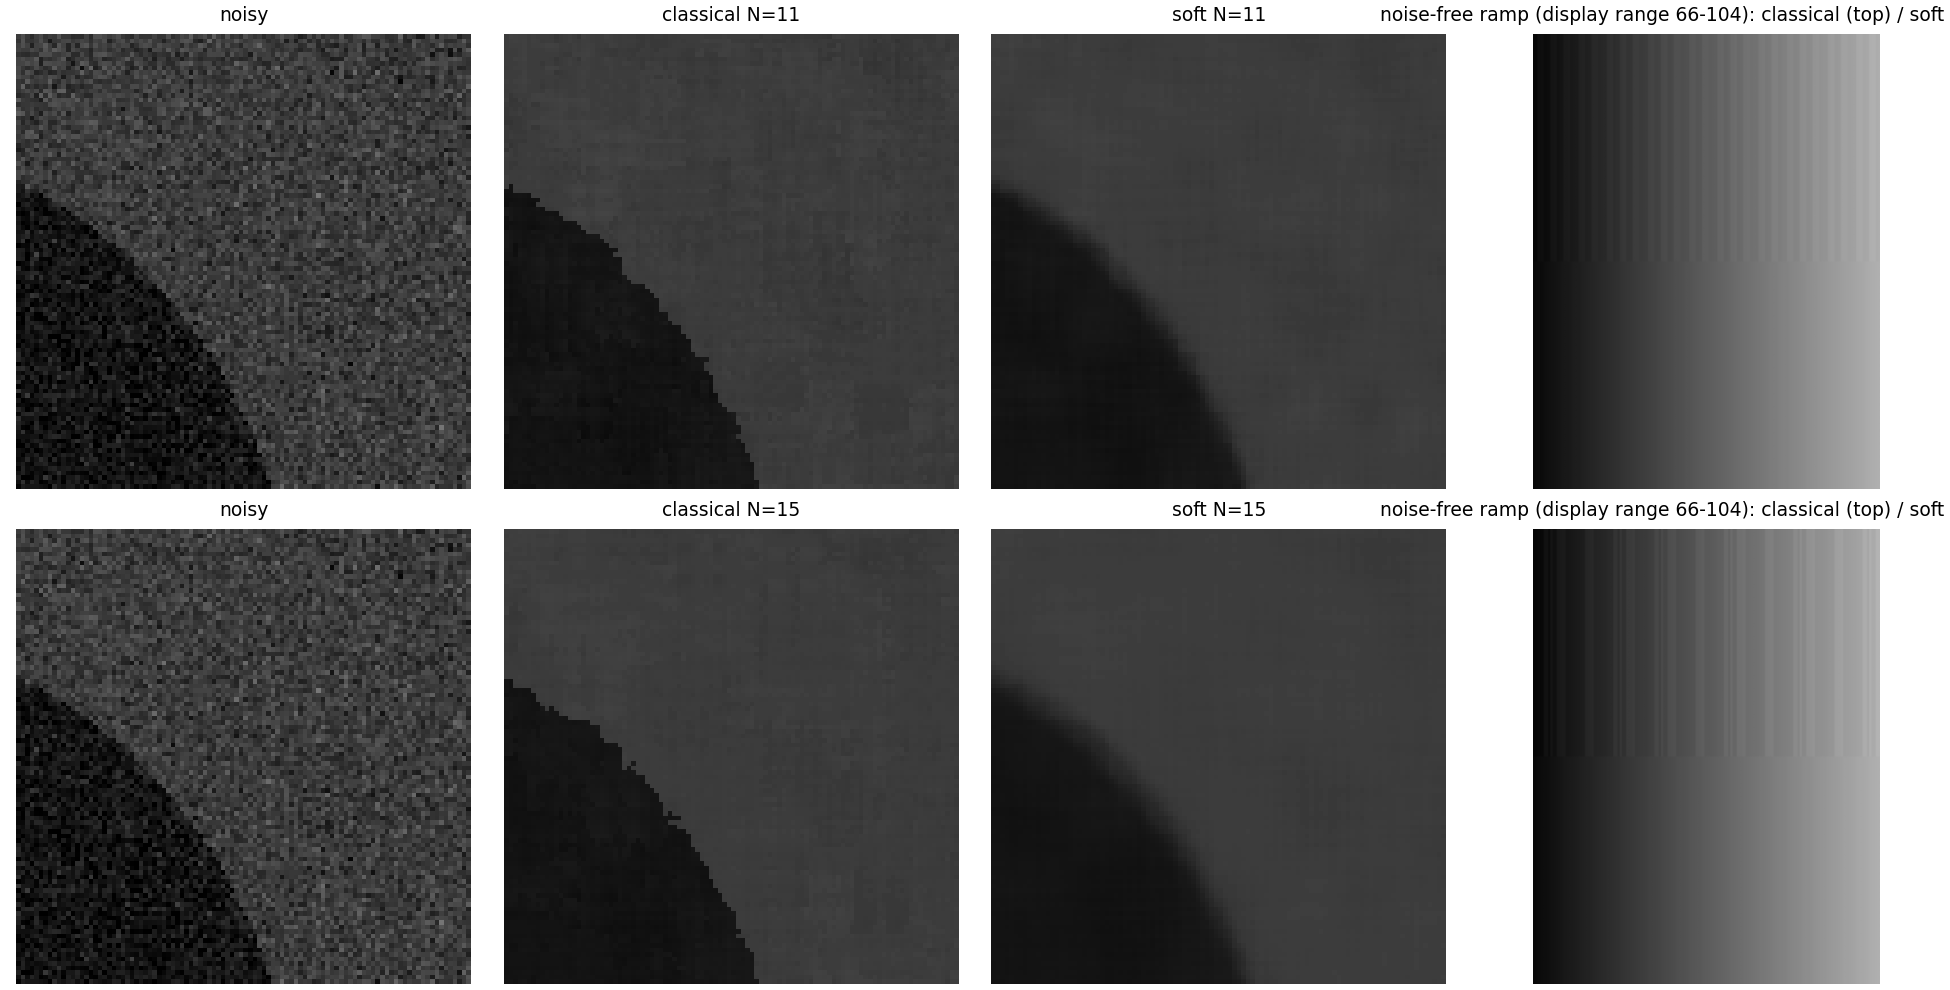
\includegraphics[width=1.00\linewidth]{q4_deblock}\par\vskip 3pt{\small\textbf{Figure 4.4.} Before/after at identical window sizes (rows N = 11 and 15): noisy crop, classical, soft; right column: the noise-free ramp (display range 66-104) processed by the classical filter (top half of each panel: irregular vertical steps, coarser for N = 15) and by the soft filter (bottom half: smooth). The classical boundary of the disc is jagged with block-shaped steps; the soft boundary is smooth but slightly displaced/blurred.\par}\end{figure}
\textbf{Reading the table.} \textit{Noise-free ramp (pure artefact).} The classical filter's artefact grows with the window size, as the assignment states: ramp RMS deviation 0.00, 0.19, 0.60 grey levels for $N=7,11,15$ and ramp gradient std 0.363, 0.453, 0.587 (the clean ramp's own value, caused by the quantisation of the 41-level ramp, is 0.363); the soft filter gives 0.26, 0.29, 0.25 grey levels and a gradient std of only 0.054, 0.027, 0.047, and the bilateral filter 0.36 grey levels and 0.009. At $N=7$ the classical filter reproduces the clean ramp exactly (RMS deviation 0.00) and is more accurate than the soft filter (its symmetric averaging adds a small bias), so de-blocking pays off only for $N\gtrsim11$; at $N=15$ the classical ramp deviation is 2.4 times larger than the soft one and its gradient std (0.587) exceeds that of the clean ramp (plateaus separated by jumps coarser than the quantisation steps). \textit{Noise-free contour.} The disc boundary of the noise-free image is displaced by 0.06 px by the classical filter and by 0.03-0.04 px by the bilateral filter, but by 0.12, 0.15, 0.40 px by the soft filter for $N=7,11,15$: the averaging rounds the boundary, the price of de-blocking (a staircase on the circle is not visible in the classical output of the clean image). The noise-free TV excess is below 0.013 for every filter and does not discriminate. \textit{Noisy input.} The classical filter displaces the contour more than the soft one (0.43 vs 0.29 px at $N=7$, 0.70 vs 0.54 px at $N=15$) and its ramp deviation and ramp gradient std are higher, but these columns mix residual noise, over-smoothing and blockiness: the soft filter reduces the TV excess by a factor of about 2.6 at $N=11$, largely because it smooths more (Table 4.1: flat-field variance ratio 0.009 vs 0.028 for the classical filter at the same $N$). The noise-free columns are therefore the clean evidence of reduced blockiness, and the soft filter's gain in PSNR/SSIM (Table 4.2) should not be attributed to de-blocking alone.

\begin{table}[H]\centering\footnotesize{\small\textbf{Table 4.6.} Soft-Kuwahara temperature sweep at N = 11 (noisy input, tau = lambda sigma-hat\textasciicircum{}2); lambda -\textgreater{} 0 recovers the classical filter.\par}\vskip 3pt
\resizebox{\ifdim\width>\linewidth\linewidth\else\width\fi}{!}{\begin{tabular}{rrrrrr}\toprule
\textbf{\begin{tabular}[b]{@{}c@{}}tau /\\{}sigma-hat\textasciicircum{}2\end{tabular}} & \textbf{PSNR} & \textbf{SSIM} & \textbf{TV excess} & \textbf{\begin{tabular}[b]{@{}c@{}}contour dev\\{}(px)\end{tabular}} & \textbf{ramp RMS dev}\\\midrule
0.0625 & 40.31 & 0.9556 & 1.27 & 0.47 & 2.23\\
0.25 & 42.13 & 0.9779 & 0.807 & 0.42 & 1.70\\
1.0 & 41.93 & 0.9815 & 0.637 & 0.32 & 1.50\\
4.0 & 40.14 & 0.9775 & 0.616 & 0.28 & 1.48\\
16.0 & 34.22 & 0.9633 & 0.614 & 0.48 & 1.48\\
\bottomrule\end{tabular}}\end{table}
\subsubsection{4.2c Per-pixel operation counts}
Counting conventions: additions include subtractions and accumulations; the spatial weights $w_s$ of the bilateral filter and all constants are precomputed (not counted); a window of $N\times N$ with sub-window $m=(N+1)/2$. \textit{Bilateral} (per neighbour: one subtraction, one squaring (multiplication), one scaling by $-1/2\sigma_r^2$, one exponential, one product $w_sw_r$, one product $wI$, two accumulations): $3N^2$ additions, $4N^2$ multiplications, $N^2$ exponentials, 1 division. \textit{Classical Kuwahara} with direct window sums (per sub-window: $m^2-1$ additions for the sum, $m^2$ multiplications and $m^2-1$ additions for the sum of squares, then the mean, its square and the variance: 3 multiplications, 1 subtraction): $4[2(m^2-1)+1]$ additions, $4(m^2+3)$ multiplications, 0 exponentials, 3 comparisons. With integral images of $I$ and $I^2$ (built once per image: 2 additions + 1 multiplication per pixel) each window sum costs 3 additions, so the count is independent of $N$ ($28$ additions, $14$ multiplications). \textit{Soft-Kuwahara} adds to Kuwahara: 4 subtractions ($\sigma_i^2-\sigma^2_{\min}$), 4 scalings by $1/\tau$, \textbf{4 exponentials}, 4 products $w_i\mu_i$, 6 additions, 1 division.

\begin{table}[H]\centering\footnotesize{\small\textbf{Table 4.7.} Operations per pixel (N is the window size; bilateral window = N x N).\par}\vskip 3pt
\resizebox{\ifdim\width>\linewidth\linewidth\else\width\fi}{!}{\begin{tabular}{rlrrrr}\toprule
\textbf{N} & \textbf{algorithm} & \textbf{additions} & \textbf{multiplications} & \textbf{exponentials} & \textbf{divisions}\\\midrule
7 & bilateral & 147 & 196 & 49 & 1\\
7 & classical Kuwahara (direct sums) & 124 & 76 & 0 & 0\\
7 & classical Kuwahara (integral images) & 28 & 14 & 0 & 0\\
7 & soft-Kuwahara (direct sums) & 134 & 84 & 4 & 1\\
7 & soft-Kuwahara (integral images) & 38 & 22 & 4 & 1\\
11 & bilateral & 363 & 484 & 121 & 1\\
11 & classical Kuwahara (direct sums) & 284 & 156 & 0 & 0\\
11 & classical Kuwahara (integral images) & 28 & 14 & 0 & 0\\
11 & soft-Kuwahara (direct sums) & 294 & 164 & 4 & 1\\
11 & soft-Kuwahara (integral images) & 38 & 22 & 4 & 1\\
15 & bilateral & 675 & 900 & 225 & 1\\
15 & classical Kuwahara (direct sums) & 508 & 268 & 0 & 0\\
15 & classical Kuwahara (integral images) & 28 & 14 & 0 & 0\\
15 & soft-Kuwahara (direct sums) & 518 & 276 & 4 & 1\\
15 & soft-Kuwahara (integral images) & 38 & 22 & 4 & 1\\
\bottomrule\end{tabular}}\end{table}
\begin{table}[H]\centering\footnotesize{\small\textbf{Table 4.8.} Measured wall time (s, median of 3, this machine, NumPy implementations on 512x512; bilateral with the matched sigma\_s of Table 4.1 and window capped at 25x25; informative only - not part of any numerical comparison).\par}\vskip 3pt
\resizebox{\ifdim\width>\linewidth\linewidth\else\width\fi}{!}{\begin{tabular}{rrrrr}\toprule
\textbf{N} & \textbf{bilateral (s)} & \textbf{Kuwahara (s)} & \textbf{soft-Kuwahara (s)} & \textbf{bilateral / Kuwahara}\\\midrule
7 & 2.52 & 0.066 & 0.092 & 38\\
11 & 7.00 & 0.065 & 0.091 & 107\\
15 & 6.99 & 0.065 & 0.093 & 108\\
\bottomrule\end{tabular}}\end{table}
\textbf{The bilateral filter is the most expensive per pixel}: its cost is $O(N^2)$ and each of the $N^2$ neighbours needs a transcendental function (the exponential, tens of cycles) plus 7 other operations, because the range weight depends on the data and cannot be precomputed, tabulated per offset or separated into 1-D passes. Kuwahara needs only means and variances, which are sums that can be obtained in $O(1)$ per pixel with integral images, independent of $N$, and has no exponentials; the soft modification adds just 4 exponentials per pixel (independent of $N$). The measured times agree in ordering (bilateral much slower than both Kuwahara variants, which are within a small factor of each other).

\subsection{4.3 Quantitative breakdown analysis of the bilateral filter}
\textbf{Synthetic step-edge generator and experiment.} A 64x64 array is split evenly into two levels $I_1=60$ (left) and $I_2=160$ (right), $|\Delta I|=100$, plus zero-mean Gaussian noise $N(0,\sigma^2)$ with $\sigma=\mathrm{NCR}\cdot|\Delta I|$; 30 values of $\mathrm{NCR}=\sigma/|\Delta I|$ are log-spaced from 0.05 to 2.0, and \textbf{every NCR uses 40 independent noise realisations} (a different random state per NCR; no fixed noisy image). Filter: bilateral with $\sigma_s\in\{1,2,3\}$ and two rules for the range scale: \textbf{rule A} $\sigma_r=2\sigma_{noise}$ (the common 'tie $\sigma_r$ to the noise' practice, used in 4.1) and \textbf{rule B} a fixed $\sigma_r=|\Delta I|/2$ independent of the noise. \textit{Edge preservation metrics:} (1) \textbf{gradient retention} $G=\max_x|\bar p(x+1)-\bar p(x)|/|\Delta I|$ where $\bar p$ is the filtered profile averaged over the central rows (8 px margin) and the 40 realisations (1 = the edge keeps its one-pixel step, \textasciitilde{}$1/(\sqrt{2\pi}\sigma_s)$ = 0.20 for $\sigma_s=2$ if smoothed like a Gaussian); (2) \textbf{edge-band PSNR}: PSNR (peak $|\Delta I|$) between filtered and clean image over the 6-pixel band centred on the edge.

\textbf{Definition of the critical threshold.} $\mathrm{NCR}^*$ is the noise-to-contrast ratio at which the gradient retention falls through 0.5 (linear interpolation in $\log\mathrm{NCR}$); this is a \textit{definition}, the curve is a smooth sigmoid and no sharp transition exists, so $\mathrm{NCR}^*$ depends on the chosen retention level (the alternative definition 'halfway between full retention and the Gaussian-smoothing limit' is also reported). For the primary configuration ($\sigma_s=2$, rule A) the measured $\mathrm{NCR}^*=0.522$.

\begin{figure}[H]\centering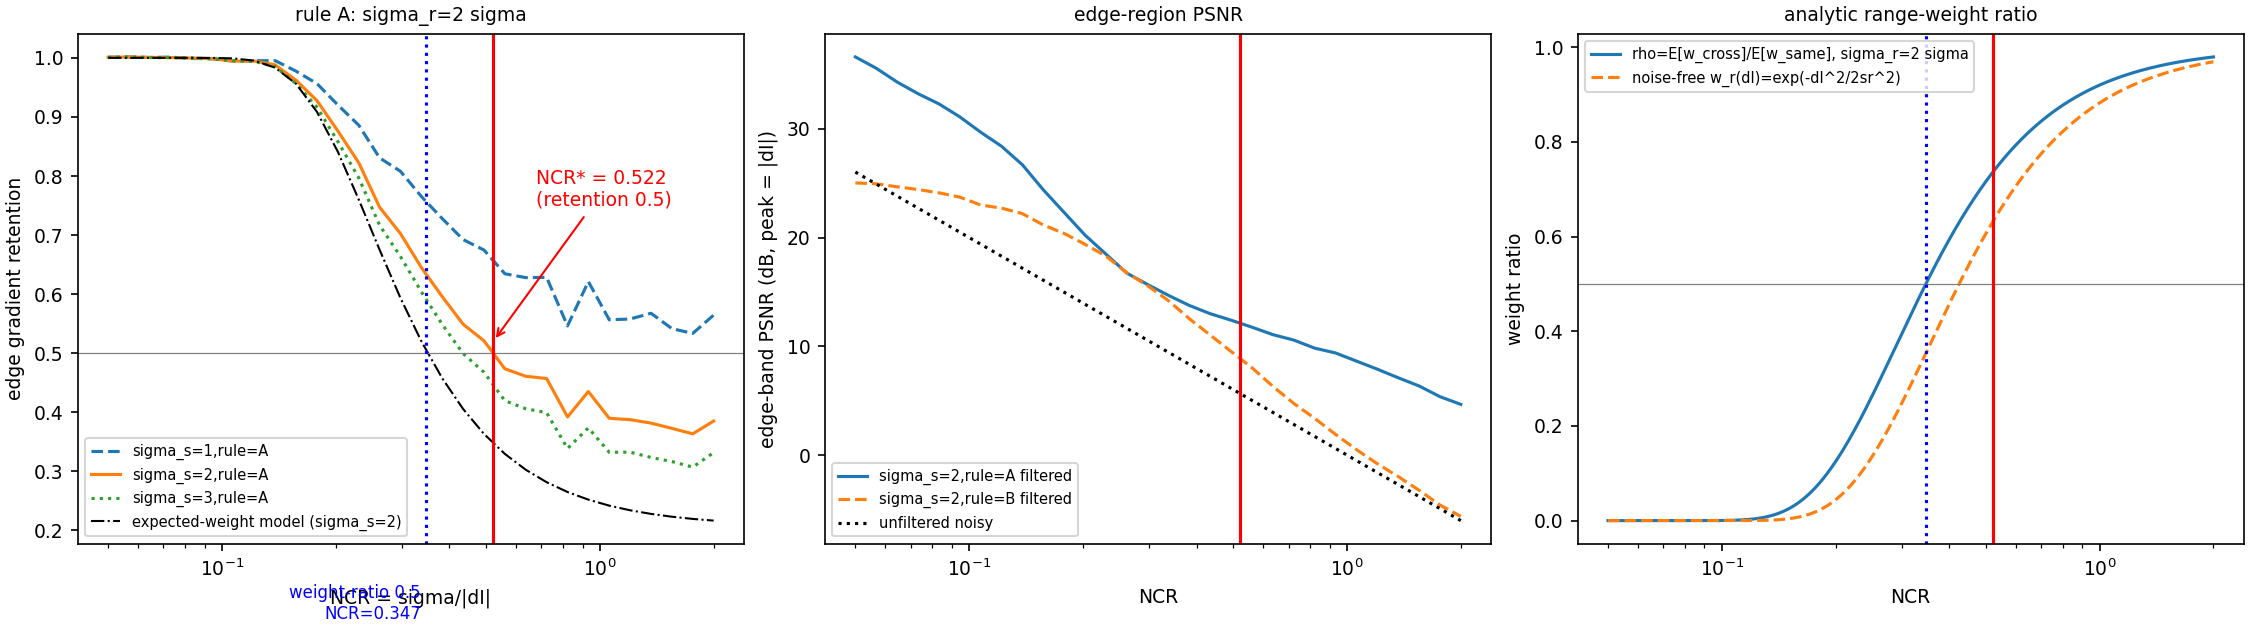
\includegraphics[width=1.00\linewidth]{q4_breakdown}\par\vskip 3pt{\small\textbf{Figure 4.5.} Left: gradient retention vs NCR (log axis) for sigma\_s = 1, 2, 3 (rule A), the expected-weight model (black dash-dot, sigma\_s = 2), the empirical NCR$^*$ (red, annotated) and the analytic weight-ratio value 0.347 (blue). Middle: edge-band PSNR vs NCR for rules A and B and the unfiltered noisy input. Right: analytic range-weight ratio, with noise in the difference (solid) and noise-free (dashed).\par}\end{figure}
\begin{table}[H]\centering\footnotesize{\small\textbf{Table 4.9.} Empirical critical thresholds (gradient retention crossing 0.5, and crossing the midpoint between 1 and the Gaussian-smoothing limit) for all six configurations. 'n/a' = the curve never crosses the level in 0.05 \textless{}= NCR \textless{}= 2.\par}\vskip 3pt
\resizebox{\ifdim\width>\linewidth\linewidth\else\width\fi}{!}{\begin{tabular}{lrrrr}\toprule
\textbf{configuration} & \textbf{retention at NCR=0.05} & \textbf{NCR$^*$ (retention = 0.5)} & \textbf{NCR$^*$ (halfway to Gaussian limit)} & \textbf{Gaussian-limit retention}\\\midrule
sigma\_s=1,rule=A & 1.001 & n/a & 0.424 & 0.399\\
sigma\_s=1,rule=B & 0.889 & n/a & n/a & 0.399\\
sigma\_s=2,rule=A & 1.001 & 0.522 & 0.379 & 0.199\\
sigma\_s=2,rule=B & 0.832 & n/a & n/a & 0.199\\
sigma\_s=3,rule=A & 1.001 & 0.434 & 0.367 & 0.133\\
sigma\_s=3,rule=B & 0.810 & n/a & n/a & 0.133\\
\bottomrule\end{tabular}}\end{table}
\begin{table}[H]\centering\small{\small\textbf{Table 4.10.} Breakdown curve for the primary configuration (sigma\_s=2, sigma\_r = 2 sigma; every third NCR value of the 30 shown; all 30 are in results/q4.json).\par}\vskip 3pt
\resizebox{\ifdim\width>\linewidth\linewidth\else\width\fi}{!}{\begin{tabular}{rrrr}\toprule
\textbf{NCR} & \textbf{gradient retention} & \textbf{edge-band PSNR filtered (dB)} & \textbf{edge-band PSNR noisy (dB)}\\\midrule
0.0500 & 1.001 & 36.60 & 26.02\\
0.0732 & 1.001 & 33.23 & 22.71\\
0.1073 & 0.994 & 29.68 & 19.39\\
0.1571 & 0.962 & 24.39 & 16.08\\
0.2301 & 0.823 & 18.48 & 12.76\\
0.3370 & 0.645 & 14.68 & 9.45\\
0.4936 & 0.521 & 12.40 & 6.13\\
0.7229 & 0.457 & 10.57 & 2.82\\
1.0588 & 0.390 & 8.64 & -0.50\\
1.5508 & 0.373 & 6.36 & -3.81\\
\bottomrule\end{tabular}}\end{table}
\subsubsection{4.3c Mathematical explanation}
\textbf{Mathematical prediction (exact, given the assumptions).} Two pixels $p,q$ on opposite sides of the edge have noisy values differing by $d=\Delta I+n_q-n_p\sim N(\Delta I,2\sigma^2)$; on the same side $d\sim N(0,2\sigma^2)$. For $w_r(d)=e^{-d^2/(2\sigma_r^2)}$ and $d\sim N(\mu,s^2)$, $E[w_r]=\sqrt{\frac{\sigma_r^2}{\sigma_r^2+s^2}}\exp\!\big(-\frac{\mu^2}{2(\sigma_r^2+s^2)}\big)$, so the \textbf{expected cross-edge to same-side weight ratio} is

\begin{equation}\rho=\frac{E[w_r]_{cross}}{E[w_r]_{same}}=\exp\!\Big(-\frac{\Delta I^{2}}{2(\sigma_r^{2}+2\sigma^{2})}\Big)\ \xrightarrow{\ \sigma_r=2\sigma\ }\ \rho=\exp\!\Big(-\frac{1}{12\,\mathrm{NCR}^{2}}\Big)\end{equation}
The \textit{noise-free} range weight $w_r(\Delta I)=e^{-\Delta I^2/(2\sigma_r^2)}=e^{-1/(8\mathrm{NCR}^2)}$ (for $\sigma_r=2\sigma$) is the quantity the question refers to; the noise in the \textit{difference of two noisy samples} adds $2\sigma^2$ to the denominator and is why 12 appears instead of 8. A Monte-Carlo check with $2\times10^6$ pairs agrees with the closed form: NCR = 0.2, 0.347, 0.5, 1.0 gives MC ratios 0.1245, 0.5005, 0.7167, 0.9200 against 0.1245, 0.5005, 0.7165, 0.9200.

\textbf{Mathematical prediction of a threshold.} The weight ratio reaches $1/2$ when $1/(12\mathrm{NCR}^2)=\ln2$, i.e. $\mathrm{NCR}_{\rho=1/2}=1/\sqrt{12\ln2}=0.3467$ (analytic; this is a statement about \textit{weights}, not about measured edge retention). As $\mathrm{NCR}\to\infty$, $\rho\to1$: the range kernel gives the same weight to neighbours across and on the same side of the edge and the bilateral filter degenerates to the Gaussian spatial filter, smoothing across the edge; as $\mathrm{NCR}\to0$, $\rho\to0$ and the edge is perfectly preserved.

\textbf{Heuristic and empirical observations (to be kept apart from the prediction).} \textit{Heuristic:} an expected-weight model replaces the random weights by their means: for a pixel at column $x$ relative to the edge, $\hat p(x)=\sum_jw_{s,j}\bar w_j\mu_j/\sum_jw_{s,j}\bar w_j$ with $\bar w_j$ the expected range weight above (the centre pixel has weight exactly 1). It ignores that the weights are random and correlated through the centre pixel's own noise. It predicts a retention-0.5 crossing at $\mathrm{NCR}=0.351$ (black curve of Figure 4.5). \textit{Empirical:} the measured retention-0.5 crossing for $\sigma_s=2$, rule A is \textbf{0.522} (and n/a for $\sigma_s=1$, 0.434 for $\sigma_s=3$; rule B: n/a, n/a, n/a for $\sigma_s=1,2,3$).

\textbf{Why the analytic weight-ratio value and the measured breakdown threshold differ.} (1) \textit{They are different quantities.} $\rho=1/2$ is a condition on the expected weights of a \textit{pair} of pixels; retention is a property of a weighted \textit{average} over a window, and the level 0.5 is itself arbitrary. (2) \textit{Window geometry alone does not explain the gap.} The expected-weight model already contains the geometry (how many neighbours lie across the edge for a pixel adjacent to it) and it predicts a retention-0.5 crossing at $\mathrm{NCR}=0.351$, almost the weight half-point 0.347, while the measured crossing is 0.522: at NCR = 0.347 the model gives retention 0.52 but the measurement 0.65. The measured filter therefore preserves the edge \textit{better} than the mean-weight model predicts. (3) What the model neglects is the randomness of the weights, and this is the likely cause: the filter weights are functions of the \textit{actual} noisy values, so for a pixel next to the edge the neighbours on the other side whose noisy value happens to lie close to the centre value receive a large weight and the others almost none; the filtered value is a ratio of random sums, whose expectation is not the ratio of the expected sums (Jensen), and the centre pixel's own noise is shared by all its weights and keeps the pixel on its own side of the step (the weights favour neighbours similar to it, i.e. noise copying). This cause was not isolated by a separate experiment (the Monte-Carlo check above verifies the pair-weight ratio, not the retention), so it is a heuristic explanation. (4) The threshold depends on the filter and the metric: 0.522 for $\sigma_s=2$, 0.434 for $\sigma_s=3$ (a larger window gives more cross-edge neighbours), no crossing at all for $\sigma_s=1$ (whose Gaussian-smoothing limit of retention is 0.40 \textless{} 0.5, so the midpoint definition applies: 0.424), and none for rule B (fixed $\sigma_r=|\Delta I|/2$ never reaches retention 0.5 in the explored range because its range kernel is independent of the noise). So neither number is 'the' threshold: 0.347 is the analytic weight-ratio half-point and 0.522 is the empirical NCR at which the edge-gradient retention of this configuration crosses 0.5. The rule of thumb that follows is that bilateral edge preservation degrades progressively as $\sigma/|\Delta I|$ grows through 0.3-0.6 and is largely lost for $\mathrm{NCR}\gtrsim1$ (retention at NCR = 1 is 0.390, against 0.20 for pure Gaussian smoothing with $\sigma_s=2$).

\begin{figure}[H]\centering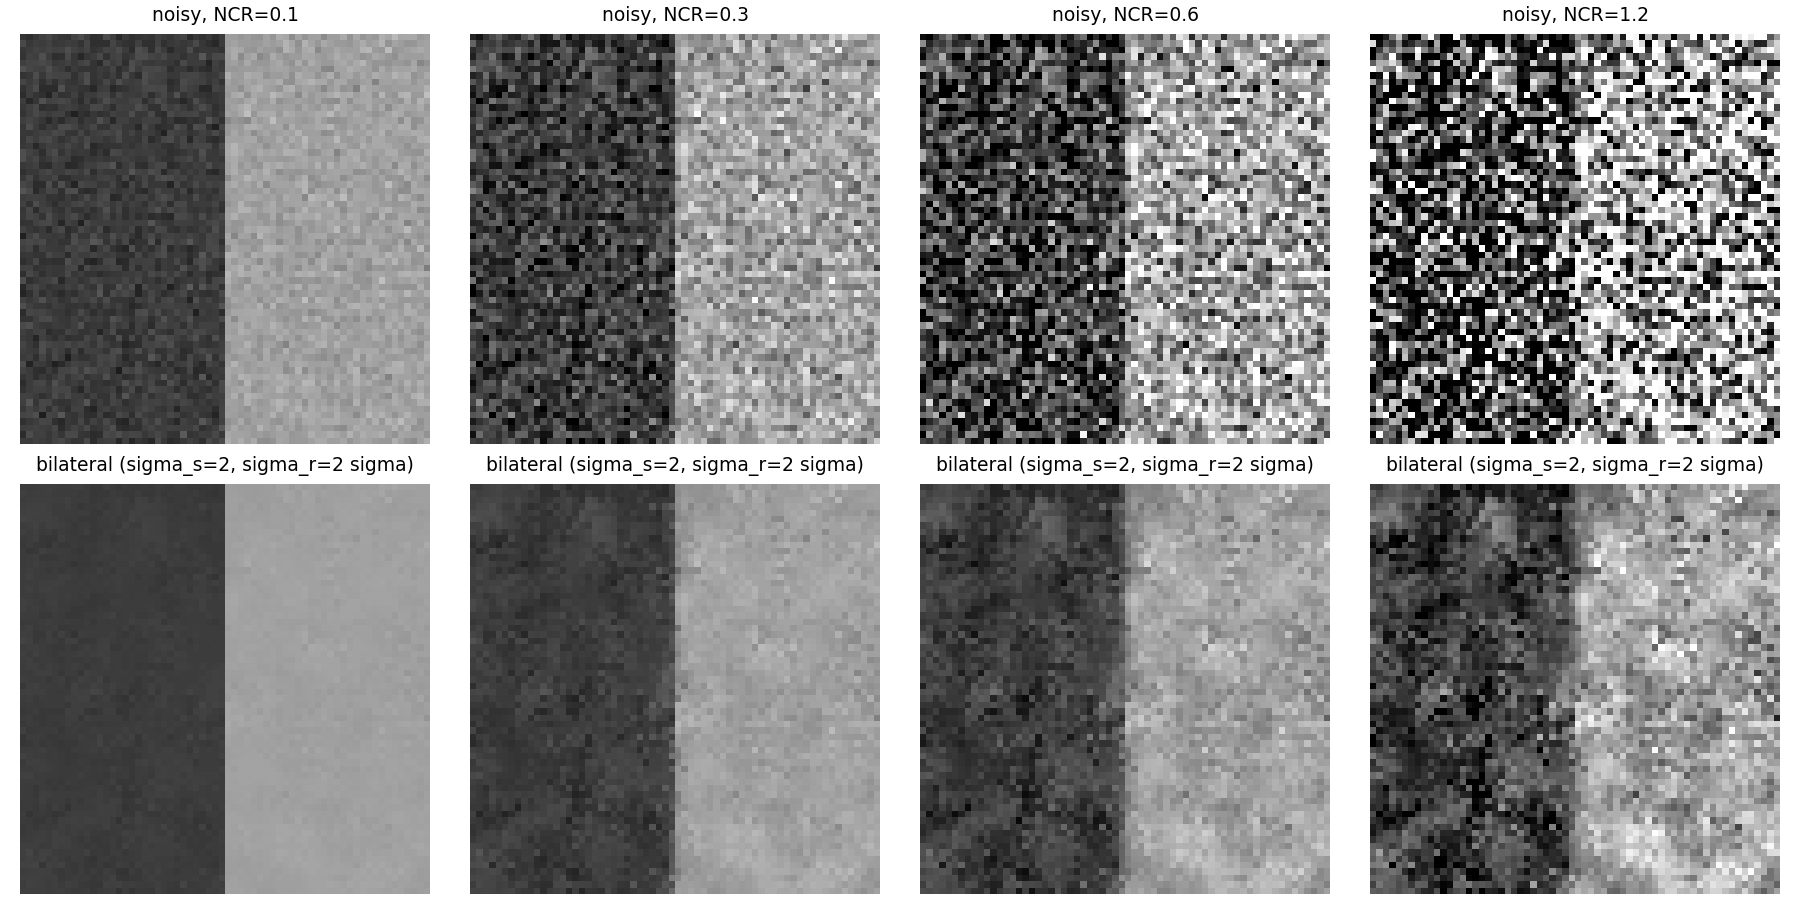
\includegraphics[width=0.85\linewidth]{q4_step_examples}\par\vskip 3pt{\small\textbf{Figure 4.6.} Synthetic step edge at NCR = 0.1, 0.3, 0.6, 1.2 (top) and the bilateral output (sigma\_s = 2, sigma\_r = 2 sigma, bottom): the edge is sharp at low NCR and disappears into the noise at high NCR.\par}\end{figure}
\section{Question 5 - Denoising and the Wiener filter}
\subsection{5.1 The Wiener filter as an MMSE denoiser}
\textbf{Derivation.} Let $g=f+n$ with $f$ and $n$ uncorrelated, zero-mean, wide-sense stationary random fields with power spectral densities $S_{ff}$, $S_{nn}$. Stationarity makes the DFT diagonalise the covariance, so the best \textit{linear} (shift-invariant) estimate is a per-frequency gain, $\hat F(u,v)=W(u,v)G(u,v)$, chosen to minimise $J(W)=E|F-WG|^2$ at each frequency. With $E|F|^2=S_{ff}$, $E|G|^2=S_{ff}+S_{nn}$ and $E[F\bar G]=S_{ff}$ (uncorrelated noise), for the real gain $W$ of a symmetric estimator

\begin{equation}J(W)=S_{ff}-2W S_{ff}+W^{2}(S_{ff}+S_{nn}),\qquad \frac{dJ}{dW}=0\ \Rightarrow\ W=\frac{S_{ff}}{S_{ff}+S_{nn}},\quad J_{\min}=\frac{S_{ff}S_{nn}}{S_{ff}+S_{nn}}\end{equation}
(the second derivative $2(S_{ff}+S_{nn})>0$ confirms a minimum). The estimate is $\hat F=\frac{S_{ff}}{S_{ff}+S_{nn}}G=\frac{\mathrm{SNR}}{\mathrm{SNR}+1}G$ with $\mathrm{SNR}(u,v)=S_{ff}/S_{nn}$: the gain is $\approx1$ where the signal dominates and $\approx\mathrm{SNR}\ll1$ where noise dominates, and the residual error $J_{\min}\le\min(S_{ff},S_{nn})$ is never worse than doing nothing or keeping nothing.

\textbf{Implementation (src/q5\_wiener.py).} Working image: the instructor-provided \texttt{reference\_\allowbreak{}image.\allowbreak{}jpg} is 3072x2048 (native, RGB); to keep the 2-D FFTs and the from-scratch bilateral filter tractable it is reduced by 2x2 block averaging to \textbf{1536x1024} (both sides \textgreater{}= 1024 as the assignment requires; the reduction is area averaging, stored as \texttt{data/\allowbreak{}derived/\allowbreak{}reference\_\allowbreak{}work\_\allowbreak{}1536x1024.\allowbreak{}png}). Intensities are normalised to [0,1] inside the Wiener filter; noise is white Gaussian with $\sigma\in\{5,10,20,40\}$ 8-bit levels, generated as $\sigma z$ from \textbf{one} unit-variance realisation $z$ (seed 2026), so every method sees the same noise at each $\sigma$; the noisy image is \textbf{not} clipped before filtering (clipping only for display and for the metrics). Each colour channel is processed independently. The channel is mirror-padded by 64 px (to a fast FFT size) to avoid wrap-around; $S_{nn}=\sigma^2$ exactly (periodogram normalisation $|G|^2/(P_rP_c)$, white noise has flat periodogram $\sigma^2$); the signal PSD is estimated from the noisy image itself: radially averaged periodogram (240 log-spaced radial bins, interpolated back to 2-D) minus $S_{nn}$, floored at $0.01\,S_{nn}$ so that $W\ge0.0099$ at the highest frequencies. \textbf{Assumptions:} (i) noise white, stationary, signal-independent and Gaussian; (ii) $f$ stationary with an \textit{isotropic} spectrum (the radial average discards the horizontal/vertical dominance of real photographs); (iii) the periodogram is a consistent estimate after radial averaging; (iv) the noise power is either known (injected $\sigma$) or estimated blindly with Immerkaer's method (Table 5.1 reports both: $\hat\sigma$ = 5.89, 10.53, 20.28, 40.12 for $\sigma=5,10,20,40$).

\textbf{Competitors.} (a) Problem 2 low-pass filters: Butterworth ($n=2$) and Gaussian (matched $D_0'=D_0/\sqrt{2\ln2}$), same formulas as \texttt{make\_\allowbreak{}filter} but with mirror padding and cutoffs in cycles/pixel; the cutoff $f_c$ is chosen from 28 log-spaced values in $[0.01,0.5]$ by maximum PSNR on a 512x512 centre crop against the clean image - \textbf{oracle-tuned}. A \textit{blind} Gaussian cutoff (the radius at which the estimated $S_{ff}$ falls below $S_{nn}$) is also reported. (b) Problem 4 bilateral filter (applied per channel), $\sigma_s\in\{1,2,3\}$, $\sigma_r\in\{1,2,3\}\sigma$ tuned on the same crop with the clean reference - \textbf{oracle-tuned}. The Wiener results use no clean-reference information (known $\sigma$ or estimated $\hat\sigma$).

\begin{table}[H]\centering\footnotesize{\small\textbf{Table 5.1.} PSNR (dB, data range 255) and SSIM (own implementation, Gaussian 11x11, sigma 1.5, mean over RGB) on the 1536x1024 working image, same noise realisation for all methods at each sigma. Oracle-tuned = parameters chosen with the clean reference on a 512x512 centre crop; the metrics are on the full image.\par}\vskip 3pt
\resizebox{\ifdim\width>\linewidth\linewidth\else\width\fi}{!}{\begin{tabular}{rlrrl}\toprule
\textbf{sigma} & \textbf{method} & \textbf{PSNR} & \textbf{SSIM} & \textbf{parameters / remark}\\\midrule
5 & noisy input & 34.29 & 0.8637 & -\\
 & Wiener (known sigma) & 36.28 & 0.9188 & S\_nn = sigma\textasciicircum{}2; blind w.r.t. the clean image\\
 & Wiener (Immerkaer sigma-hat = 5.89) & 36.01 & 0.9249 & fully blind\\
 & Butterworth n=2 (oracle-tuned) & 36.16 & 0.9122 & f\_c = 0.500 cyc/px (grid edge)\\
 & Gaussian matched (oracle-tuned) & 36.17 & 0.9173 & f\_c(half-amplitude) = 0.500 cyc/px (grid edge)\\
 & Gaussian, blind cutoff (S\_ff = S\_nn) & 36.17 & 0.9183 & f\_c = 0.489 cyc/px\\
 & Bilateral (oracle-tuned) & 37.07 & 0.9387 & sigma\_s = 1, sigma\_r = 2 sigma\\
10 & noisy input & 28.41 & 0.6560 & -\\
 & Wiener (known sigma) & 32.37 & 0.8392 & S\_nn = sigma\textasciicircum{}2; blind w.r.t. the clean image\\
 & Wiener (Immerkaer sigma-hat = 10.53) & 32.32 & 0.8453 & fully blind\\
 & Butterworth n=2 (oracle-tuned) & 32.29 & 0.8345 & f\_c = 0.324 cyc/px\\
 & Gaussian matched (oracle-tuned) & 32.35 & 0.8373 & f\_c(half-amplitude) = 0.324 cyc/px\\
 & Gaussian, blind cutoff (S\_ff = S\_nn) & 32.31 & 0.8308 & f\_c = 0.343 cyc/px\\
 & Bilateral (oracle-tuned) & 33.14 & 0.8679 & sigma\_s = 1, sigma\_r = 3 sigma\\
20 & noisy input & 22.66 & 0.3828 & -\\
 & Wiener (known sigma) & 29.31 & 0.7376 & S\_nn = sigma\textasciicircum{}2; blind w.r.t. the clean image\\
 & Wiener (Immerkaer sigma-hat = 20.28) & 29.30 & 0.7409 & fully blind\\
 & Butterworth n=2 (oracle-tuned) & 29.12 & 0.7296 & f\_c = 0.210 cyc/px\\
 & Gaussian matched (oracle-tuned) & 29.27 & 0.7332 & f\_c(half-amplitude) = 0.210 cyc/px\\
 & Gaussian, blind cutoff (S\_ff = S\_nn) & 29.27 & 0.7373 & f\_c = 0.202 cyc/px\\
 & Bilateral (oracle-tuned) & 29.38 & 0.7238 & sigma\_s = 1, sigma\_r = 3 sigma\\
40 & noisy input & 17.17 & 0.1713 & -\\
 & Wiener (known sigma) & 26.99 & 0.6379 & S\_nn = sigma\textasciicircum{}2; blind w.r.t. the clean image\\
 & Wiener (Immerkaer sigma-hat = 40.12) & 26.99 & 0.6393 & fully blind\\
 & Butterworth n=2 (oracle-tuned) & 26.73 & 0.6402 & f\_c = 0.102 cyc/px\\
 & Gaussian matched (oracle-tuned) & 26.86 & 0.6353 & f\_c(half-amplitude) = 0.117 cyc/px\\
 & Gaussian, blind cutoff (S\_ff = S\_nn) & 26.82 & 0.6411 & f\_c = 0.102 cyc/px\\
 & Bilateral (oracle-tuned) & 26.79 & 0.6060 & sigma\_s = 2, sigma\_r = 3 sigma\\
\bottomrule\end{tabular}}\end{table}
\begin{figure}[H]\centering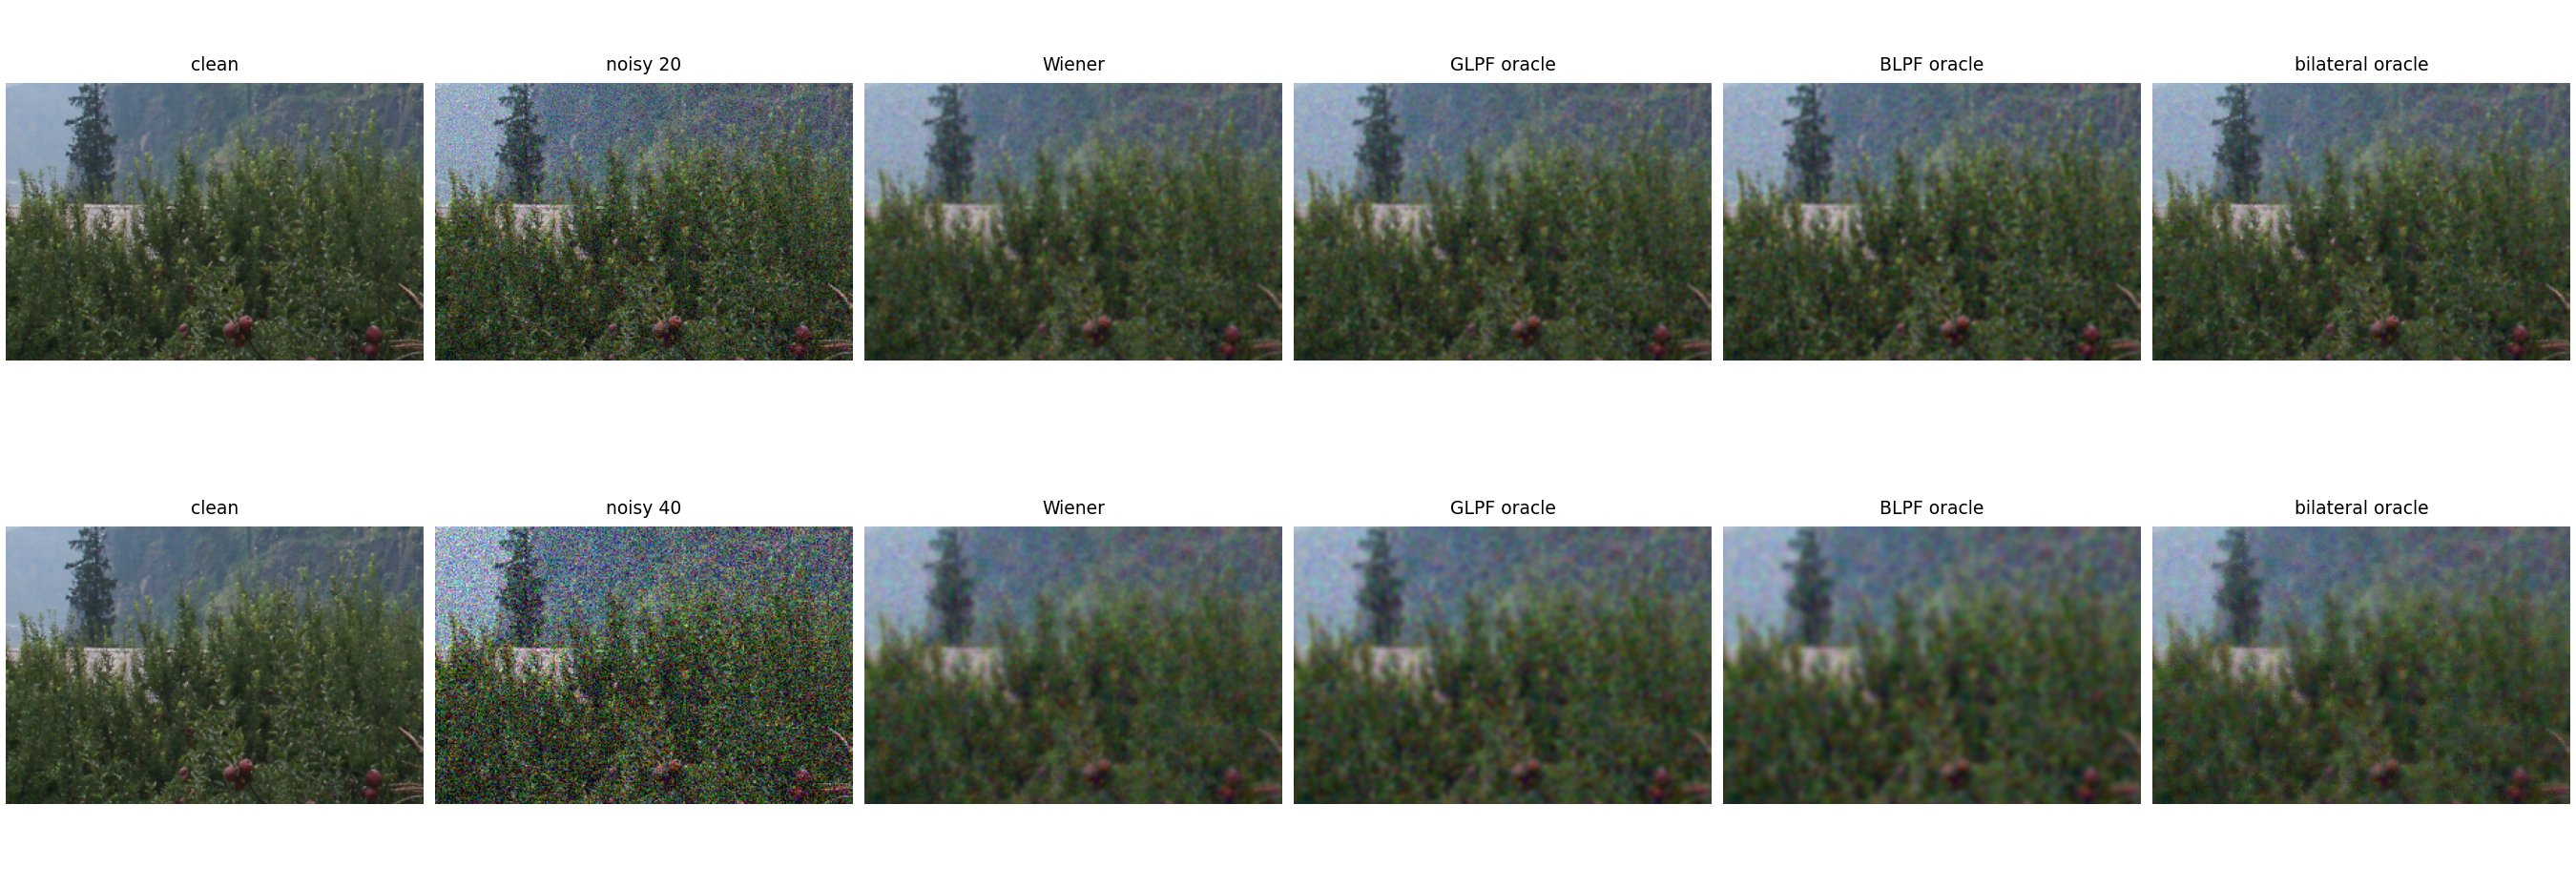
\includegraphics[width=1.00\linewidth]{q5_comparison_crops}\par\vskip 3pt{\small\textbf{Figure 5.1.} Crops (200x300 px) at sigma = 20 (top) and 40 (bottom): clean, noisy, Wiener, Gaussian (oracle), Butterworth (oracle), bilateral (oracle).\par}\end{figure}
\begin{figure}[H]\centering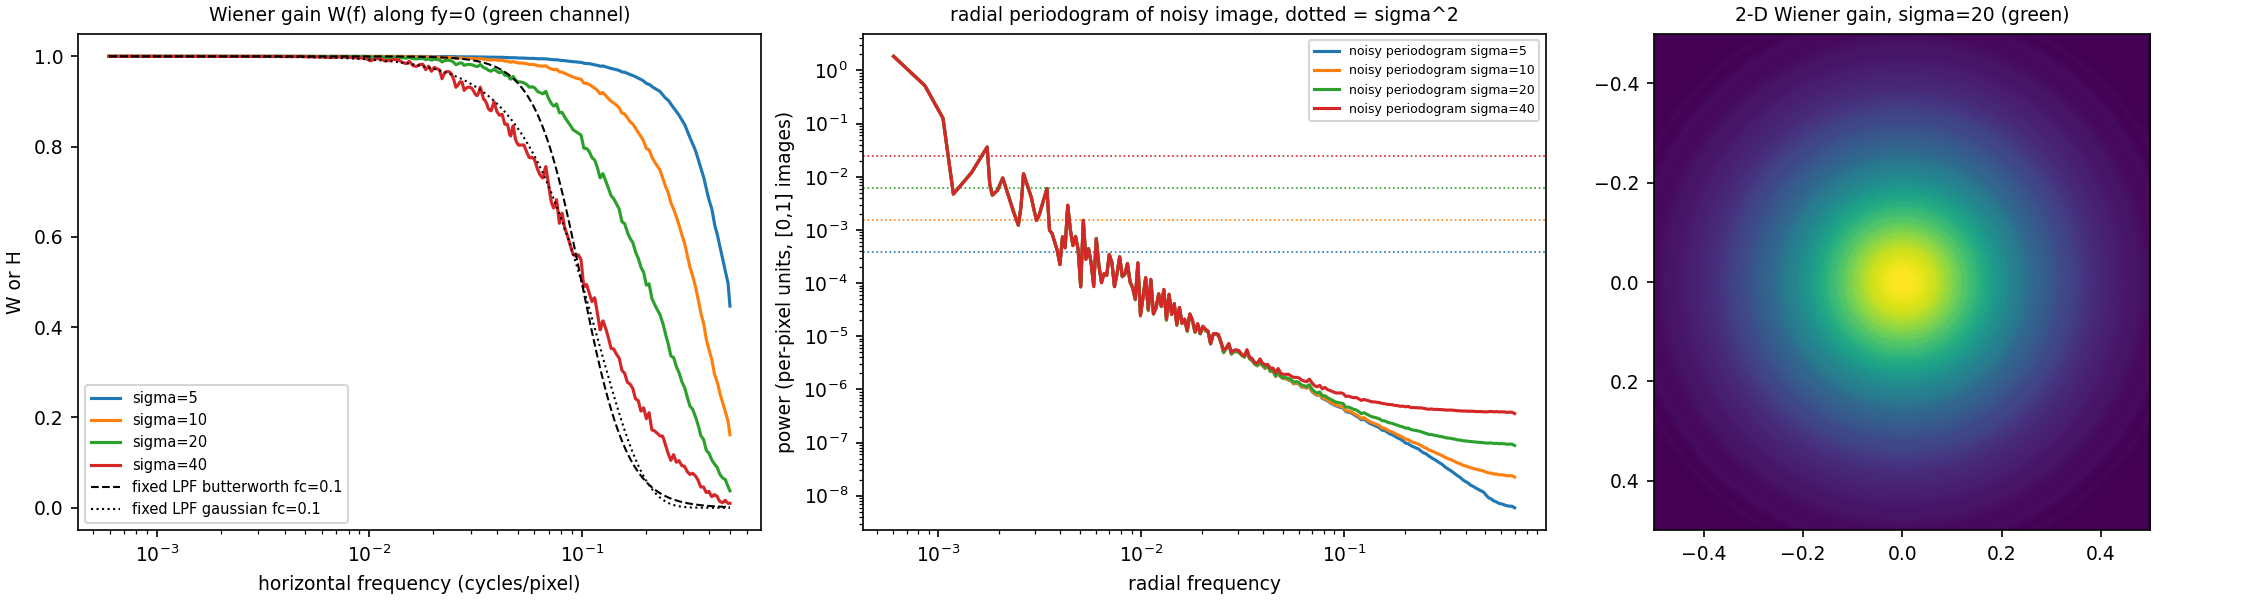
\includegraphics[width=1.00\linewidth]{q5_wiener_gain}\par\vskip 3pt{\small\textbf{Figure 5.2.} Left: Wiener gain W(f) along the horizontal frequency axis for each sigma (green channel) and two fixed low-pass filters (dashed, f\_c = 0.1). Middle: radial periodogram of the noisy image with the white level sigma\textasciicircum{}2 (dotted). Right: 2-D Wiener gain at sigma = 20.\par}\end{figure}
\textbf{How the shrinkage changes with frequency and noise power.} $W(f)=1/(1+1/\mathrm{SNR}(f))$: close to 1 at low frequency where the periodogram is orders of magnitude above $\sigma^2$, then decreasing monotonically through $W=1/2$ at the frequency where $S_{ff}=S_{nn}$ and approaching $S_{ff}/S_{nn}$ beyond (Figure 5.2). When $\sigma$ grows the white level $\sigma^2$ moves up, the crossing moves to lower frequency: the blind crossing radii are 0.489, 0.343, 0.202, 0.102 cycles/pixel for $\sigma=5,10,20,40$, i.e. the Wiener filter automatically tightens its bandwidth by a factor of about 4.8 over this range. \textbf{Difference from a fixed-cutoff low-pass:} a fixed filter has a prescribed shape (flat passband, one transition width, a single cutoff chosen by the user, ideal: 0/1) that does not depend on the data; the Wiener gain follows the \textit{estimated image spectrum}: it has no sharp cutoff, it attenuates gradually exactly where the SNR degrades, and it keeps components above the 'cutoff' if they are strong (e.g. along the dominant horizontal/vertical edge directions in the 2-D gain of Figure 5.2 right, if an anisotropic $S_{ff}$ estimate were used; the radial average used here makes the gain isotropic). If $S_{ff}$ were a step in frequency the Wiener filter would reduce to an ideal low-pass.

\textbf{Results and what they do (not) show.} Without access to the clean image the Wiener filter gains 1.99, 3.97, 6.65, 9.81 dB over the noisy input for $\sigma=5,10,20,40$ and is within 0.3 dB of the \textit{oracle-tuned} Butterworth/Gaussian low-pass filters at every noise level (+0.12, +0.09, +0.18, +0.25 dB over the oracle Butterworth); at $\sigma=5$ the oracle cutoff is at the edge of the search grid (0.5 cycles/pixel), so this one comparison is not a clean optimum. The blind Gaussian cutoff from the $S_{ff}=S_{nn}$ crossing gets within 0.2 dB of the Wiener result at all $\sigma$, which shows that for a \textit{linear, isotropic} filter most of the benefit comes from locating the right bandwidth. The \textbf{bilateral filter wins on PSNR and SSIM at }$\sigma=5,10$ (37.07 vs 36.28 dB and 33.14 vs 32.37 dB, SSIM 0.939/0.868 vs 0.919/0.839) and on PSNR at $\sigma=20$ (29.38 vs 29.31 dB, with \textit{lower} SSIM, 0.724 vs 0.738); only at the highest noise level $\sigma=40$ does Wiener beat it in PSNR (26.99 vs 26.79 dB) and SSIM (0.638 vs 0.606). The comparison is moreover tilted towards the bilateral filter: its two parameters were oracle-tuned with the clean image while the Wiener filter used none. So \textbf{Wiener does not win every comparison}, consistent with the theory: its optimality is for \textit{linear} estimators under stationary second-order statistics, whereas the bilateral filter is nonlinear, adapts locally to edges (images are not stationary), and can exceed the linear MMSE bound on PSNR; where noise is so strong that the range term can no longer separate edges from noise ($\sigma=40$ is $\mathrm{NCR}=0.4$ for an edge of contrast 100 grey levels and larger for weaker edges, cf. Section 4.3) the advantage disappears.

\subsection{5.2a Noise-power mis-specification and edge blur}
\textbf{Wrong noise power.} At $\sigma=20$ the Wiener filter was re-run assuming noise power $\kappa S_{nn}$ with $\kappa\in\{0.5,1,2\}$: $W_\kappa=\frac{S_{ff}}{S_{ff}+\kappa S_{nn}}$. Two variants are reported: (A) the signal PSD estimate is unchanged (it was obtained with the correct $S_{nn}$) and only the denominator is mis-specified - this isolates the formula; (B) the signal PSD is re-estimated by subtracting the \textit{assumed} noise power, $S_{ff}^{(\kappa)}=\bar P-\kappa S_{nn}$, which is what a user who believes the wrong $\sigma$ would actually do, giving $W=1-\kappa S_{nn}/\bar P$. Residual noise is measured as the standard deviation of (output - clean) in the flattest 48x48 clean-image block (the noisy input has 19.8 there) and edge preservation as the mean gradient magnitude of the output over the strongest 5\% clean-gradient pixels relative to the clean image.

\begin{table}[H]\centering\footnotesize{\small\textbf{Table 5.2.} Noise-power mis-specification at sigma = 20 (1536x1024 reference). The 1.0 rows are the correctly specified filter (identical in both variants).\par}\vskip 3pt
\resizebox{\ifdim\width>\linewidth\linewidth\else\width\fi}{!}{\begin{tabular}{lrrrrr}\toprule
\textbf{variant} & \textbf{\begin{tabular}[b]{@{}c@{}}assumed\\{}noise power\\{}/ true\end{tabular}} & \textbf{PSNR} & \textbf{SSIM} & \textbf{\begin{tabular}[b]{@{}c@{}}residual\\{}noise std in\\{}flat patch\end{tabular}} & \textbf{\begin{tabular}[b]{@{}c@{}}edge\\{}gradient\\{}retention\end{tabular}}\\\midrule
A (S\_ff fixed) & 0.5 & 28.95 & 0.6999 & 7.65 & 0.599\\
A (S\_ff fixed) & 1.0 & 29.31 & 0.7376 & 5.96 & 0.475\\
A (S\_ff fixed) & 2.0 & 29.03 & 0.7484 & 4.55 & 0.358\\
B (S\_ff refit) & 0.5 & 26.40 & 0.5475 & 12.11 & 0.746\\
B (S\_ff refit) & 1.0 & 29.31 & 0.7376 & 5.96 & 0.475\\
B (S\_ff refit) & 2.0 & 27.98 & 0.7080 & 3.47 & 0.232\\
\bottomrule\end{tabular}}\end{table}
\begin{figure}[H]\centering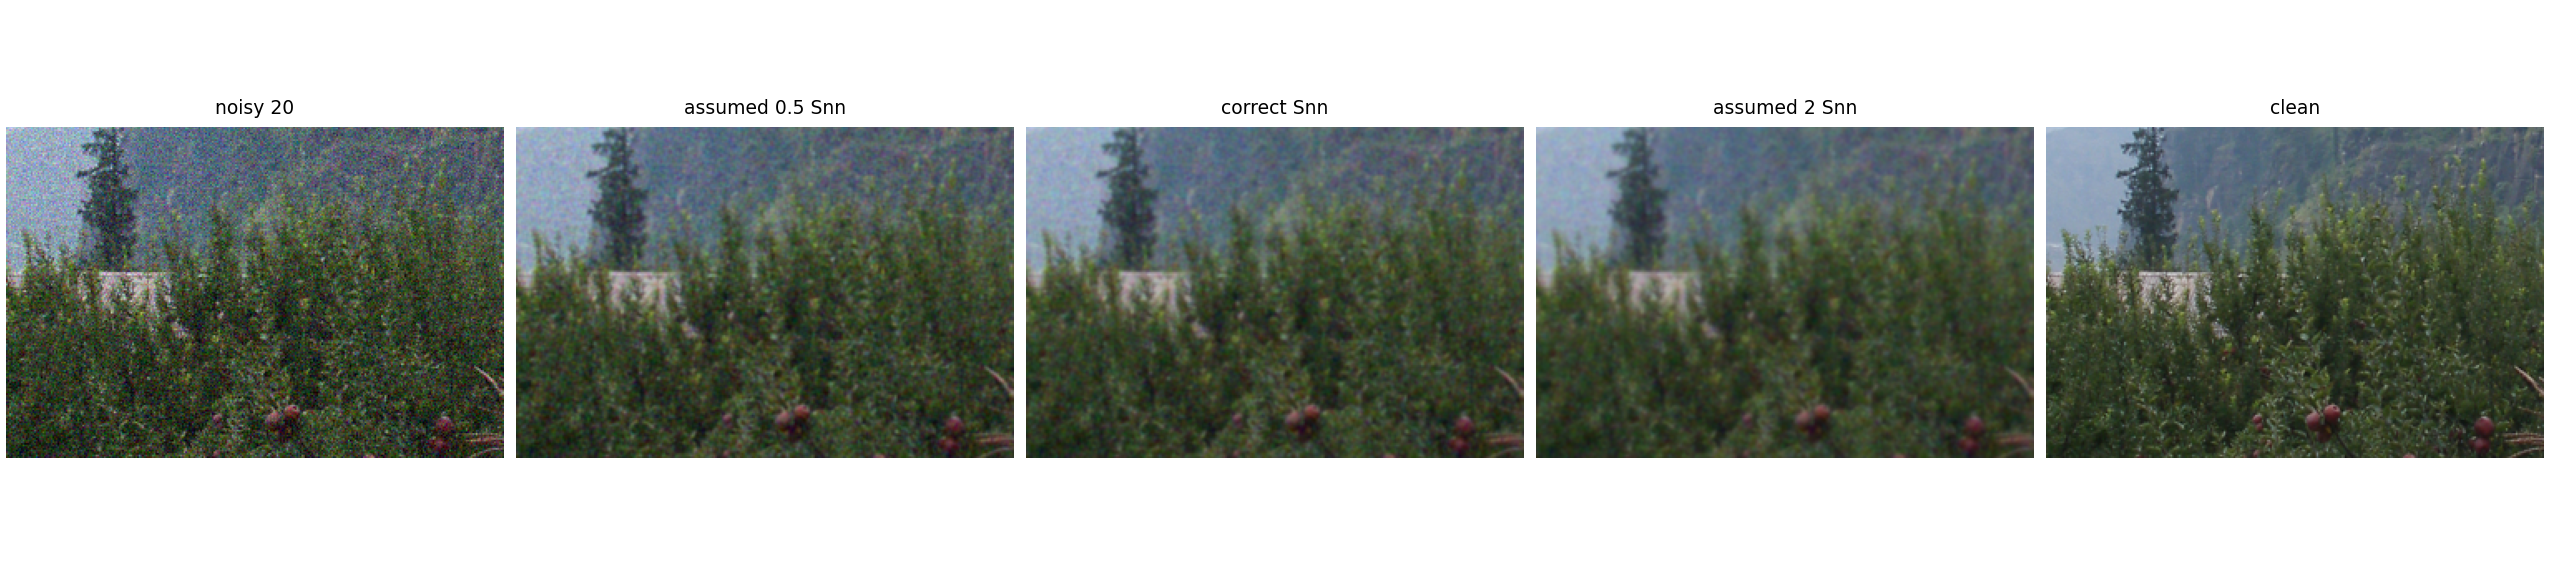
\includegraphics[width=1.00\linewidth]{q5_misestimation}\par\vskip 3pt{\small\textbf{Figure 5.3.} Noise-power mis-estimation at sigma = 20 (crop): noisy, 0.5 S\_nn, correct S\_nn, 2 S\_nn, clean.\par}\end{figure}
\textbf{Explanation.} With $0.5S_{nn}$ the gain $W_{0.5}=S_{ff}/(S_{ff}+0.5S_{nn})$ is larger than the correct one at every frequency, most where $S_{ff}\approx S_{nn}$ (the transition band), so more noise passes: the flat-patch residual noise rises from 5.96 to 7.65 grey levels and the picture looks grainy, while edges are better preserved (gradient retention 0.599 vs 0.475); the PSNR drops by 0.36 dB. With $2S_{nn}$ the gain is smaller (cutoff moves to lower frequency): residual noise falls to 4.55 but signal is removed as well - smoother, more blurred (edge retention 0.358) - and PSNR drops by 0.28 dB. SSIM \textit{increases} from 0.7376 to 0.7484 at $2S_{nn}$ because SSIM penalises residual noise in flat regions (which dominate the image) more than blur of the sparse edges, a case where the two metrics disagree. The penalty is asymmetric: the MSE-optimal setting is the correct one (PSNR 29.31 dB) and the loss is small (\textless{}0.4 dB) for a factor-of-two error in either direction since $J(W)$ is flat near its minimum, but it is larger when the noise power is under-estimated \textit{and} the signal PSD is re-fitted with the same wrong value (variant B: -2.90 dB at $0.5\times$ and -1.33 dB at $2\times$), because then both $S_{ff}$ and $S_{nn}$ are biased.

\textbf{Why a correctly specified Wiener filter still blurs edges.} The estimator is one fixed zero-phase transfer function $W(u,v)$ applied to every pixel, i.e. a convolution with the \textit{same} kernel everywhere; it is optimal for the \textit{ensemble-average} mean-square error of a stationary field. A step edge is a non-stationary event: its energy is spread over all frequencies ($\propto1/f$) and at the frequencies where $S_{ff}(f)<S_{nn}$ the filter must attenuate (the edge's high frequencies are indistinguishable, on average, from noise), so the edge is blurred whatever the local situation; averaged over all pixels this is MSE-optimal because most pixels are flat. The theory promises the minimal \textit{average} squared error among linear filters; it says nothing about edge sharpness, local error, or perceptual quality (the error map of a Wiener result is concentrated at edges), and it assumes second-order statistics only (a Gaussian field has no edges). Measured at $\sigma=20$: the correctly specified filter retains only 0.475 of the mean gradient magnitude at the strongest edges; its spatial kernel (inverse DFT of $W$) has unit sum, peak 0.215 and half-maximum width 1 px, with negligible side lobes ($|\min|/\max=1.7e-03$): a mild, essentially positive low-pass, so there is no ringing but there is blur.

\subsection{5.2b White-noise Wiener filtering of a genuinely noisy photograph}
\textbf{Photographs.} Photograph B (\texttt{IMG\_\allowbreak{}20261026\_\allowbreak{}195556198.\allowbreak{}jpg}, 4080x3072, EXIF \textbf{ISO 6400}, 1/16.7 s, f/1.87, BrightnessValue -4.6: a dark room lit by a few windows/lights) is the real low-light photo; photograph A (\texttt{IMG\_\allowbreak{}20261026\_\allowbreak{}195540763.\allowbreak{}jpg}, ISO 734, 1/14 s, BrightnessValue -0.9) shows the same room much brighter and is used only for a \textit{qualitative} comparison of noise statistics. They are \textit{not} a registered clean/noisy pair (different exposure, illumination colour and framing), so \textbf{no PSNR, SSIM or MSE is computed between them or between either and any denoised result}. Low exposure alone does not establish sensor noise; the evidence below is a direct measurement in flat regions.

\textbf{Noise-power estimation (no reference needed).} (1) Flat-region estimator: the frame is divided into non-overlapping 24x24 patches (patches whose mean is outside 8-245 are discarded because of clipping); a plane is fitted by least squares and removed from each patch; the noise standard deviation of a patch is the residual standard deviation with the $(n-3)$ degrees-of-freedom correction; the flattest 10\% of patches (smallest mean absolute 3x3 Laplacian) are kept and the median is reported per channel. (2) Immerkaer's Laplacian estimator on the whole frame as a cross-check. (3) A \textit{noise-level function}: the same patch statistic versus patch mean level (green channel, flattest 25\% of patches).

\begin{table}[H]\centering\footnotesize{\small\textbf{Table 5.3.} Noise standard deviation (8-bit grey levels) of the original 4080x3072 photographs: flat-patch estimator per channel (median of the flattest 10\% of 24x24 patches, with the inter-quartile range) and Immerkaer's whole-frame estimate.\par}\vskip 3pt
\resizebox{\ifdim\width>\linewidth\linewidth\else\width\fi}{!}{\begin{tabular}{llrrrrr}\toprule
\textbf{photo} & \textbf{channel} & \textbf{flat patches} & \textbf{\begin{tabular}[b]{@{}c@{}}their mean\\{}level\end{tabular}} & \textbf{\begin{tabular}[b]{@{}c@{}}sigma\\{}flat-patch\\{}(median)\end{tabular}} & \textbf{IQR} & \textbf{\begin{tabular}[b]{@{}c@{}}sigma\\{}Immerkaer\end{tabular}}\\\midrule
A (ISO 734) & R & 2188 & 32.2 & 0.65 & 0.58-0.75 & 0.51\\
A (ISO 734) & G & 2181 & 29.6 & 0.64 & 0.58-0.72 & 0.51\\
A (ISO 734) & B & 2180 & 28.0 & 0.67 & 0.60-0.78 & 0.51\\
B (ISO 6400) & R & 2084 & 13.2 & 2.05 & 1.74-2.40 & 1.41\\
B (ISO 6400) & G & 2029 & 14.0 & 2.33 & 2.01-2.62 & 1.41\\
B (ISO 6400) & B & 1993 & 17.4 & 2.49 & 2.26-2.73 & 1.41\\
\bottomrule\end{tabular}}\end{table}
\begin{table}[H]\centering\footnotesize{\small\textbf{Table 5.4.} Noise-level function (green channel): median detrended patch std in bins of patch mean level (flattest 25\% of patches) for A and B and their ratio. Noise grows with signal level in both images (signal-dependent, shot-noise-like) and the ratio at matched level is the like-for-like comparison. The brightest bin of B contains only 70 patches (light sources, clipped/JPEG-processed) and is not reliable.\par}\vskip 3pt
\resizebox{\ifdim\width>\linewidth\linewidth\else\width\fi}{!}{\begin{tabular}{rrrrrr}\toprule
\textbf{level range} & \textbf{sigma A} & \textbf{patches A} & \textbf{sigma B} & \textbf{patches B} & \textbf{ratio B/A}\\\midrule
8-30 & 0.64 & 1420 & 2.53 & 2806 & 3.97\\
30-60 & 0.70 & 1340 & 2.71 & 1209 & 3.89\\
60-100 & 0.90 & 433 & 2.94 & 291 & 3.25\\
100-150 & 0.90 & 1103 & 2.96 & 697 & 3.29\\
150-245 & 0.84 & 1159 & 8.17 & 70 & 9.70\\
\bottomrule\end{tabular}}\end{table}
\textbf{Findings.} Photograph B has a flat-patch noise standard deviation of about 2.0-2.5 grey levels (R/G/B medians 2.05/2.33/2.49) against 0.64-0.67 for A. At matched signal levels the ratio B/A is 4.0, 3.9, 3.3, 3.3 (in the four reliable level bins), i.e. roughly \textbf{3.3-4x} - noticeably more than the ratio 2.8 of the Immerkaer whole-frame estimates. The discrepancy between estimators is not random: the Immerkaer operator is a high-pass Laplacian and under-estimates noise that is spatially correlated (see below), while the flat-patch statistic includes all frequencies. The ISO ratio is 6400/734 = 8.7; shot-noise-limited sensors scale noise with $\sqrt{\text{gain}}=2.95$ and read-noise-limited ones with the gain, so 3.3-4 is physically plausible, but the in-camera processing (denoising, multi-frame stacking, JPEG) is unknown, so no sensor-level claim is made. In absolute terms the noise of B is small (about 1\% of full scale, 2.5-3 grey levels), smaller than the weakest synthetic case ($\sigma=5$) of Section 5.1.

\begin{figure}[H]\centering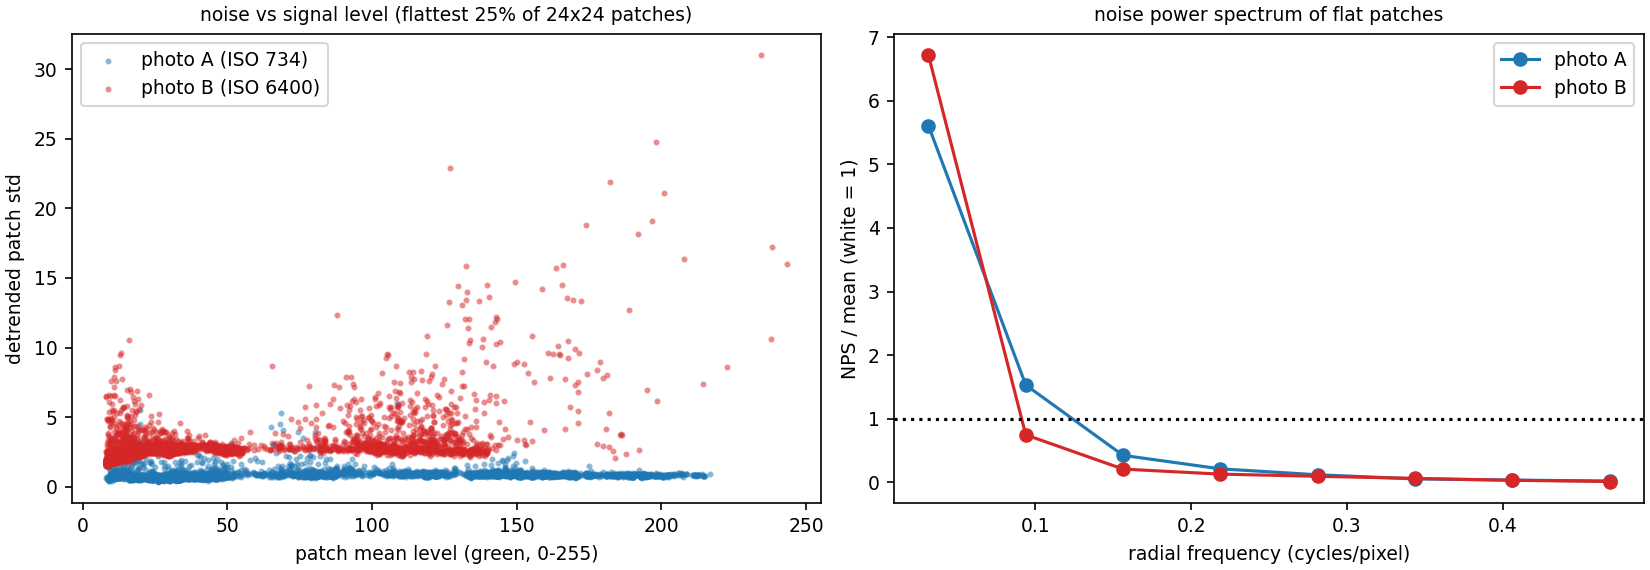
\includegraphics[width=1.00\linewidth]{q5_real_noise_analysis}\par\vskip 3pt{\small\textbf{Figure 5.4.} Left: detrended patch standard deviation vs patch mean level for A and B (green channel; flattest 25\% of patches). Right: radially averaged noise power spectrum of flat 32x32 patches (8 bands up to 0.5 cycles/pixel, normalised to the mean; white noise = 1).\par}\end{figure}
\textbf{Application of the white-noise Wiener filter.} A 1024x1024 native-resolution crop (rows 700-1723, cols 1500-2523: window lights, curtain, dark wall) of each photograph was processed per channel with the Wiener filter of 5.1 using the flat-patch noise estimate of the \textit{crop} ($\hat\sigma_{RGB}$ = 2.86, 2.91, 2.89 for B, 1.04, 1.02, 1.05 for A; the crop contains brighter regions than the frame average so the values exceed the frame-wide medians). Figure 5.5 shows the crop, a zoom before/after and the residual (noisy minus denoised, amplified x4).

\begin{figure}[H]\centering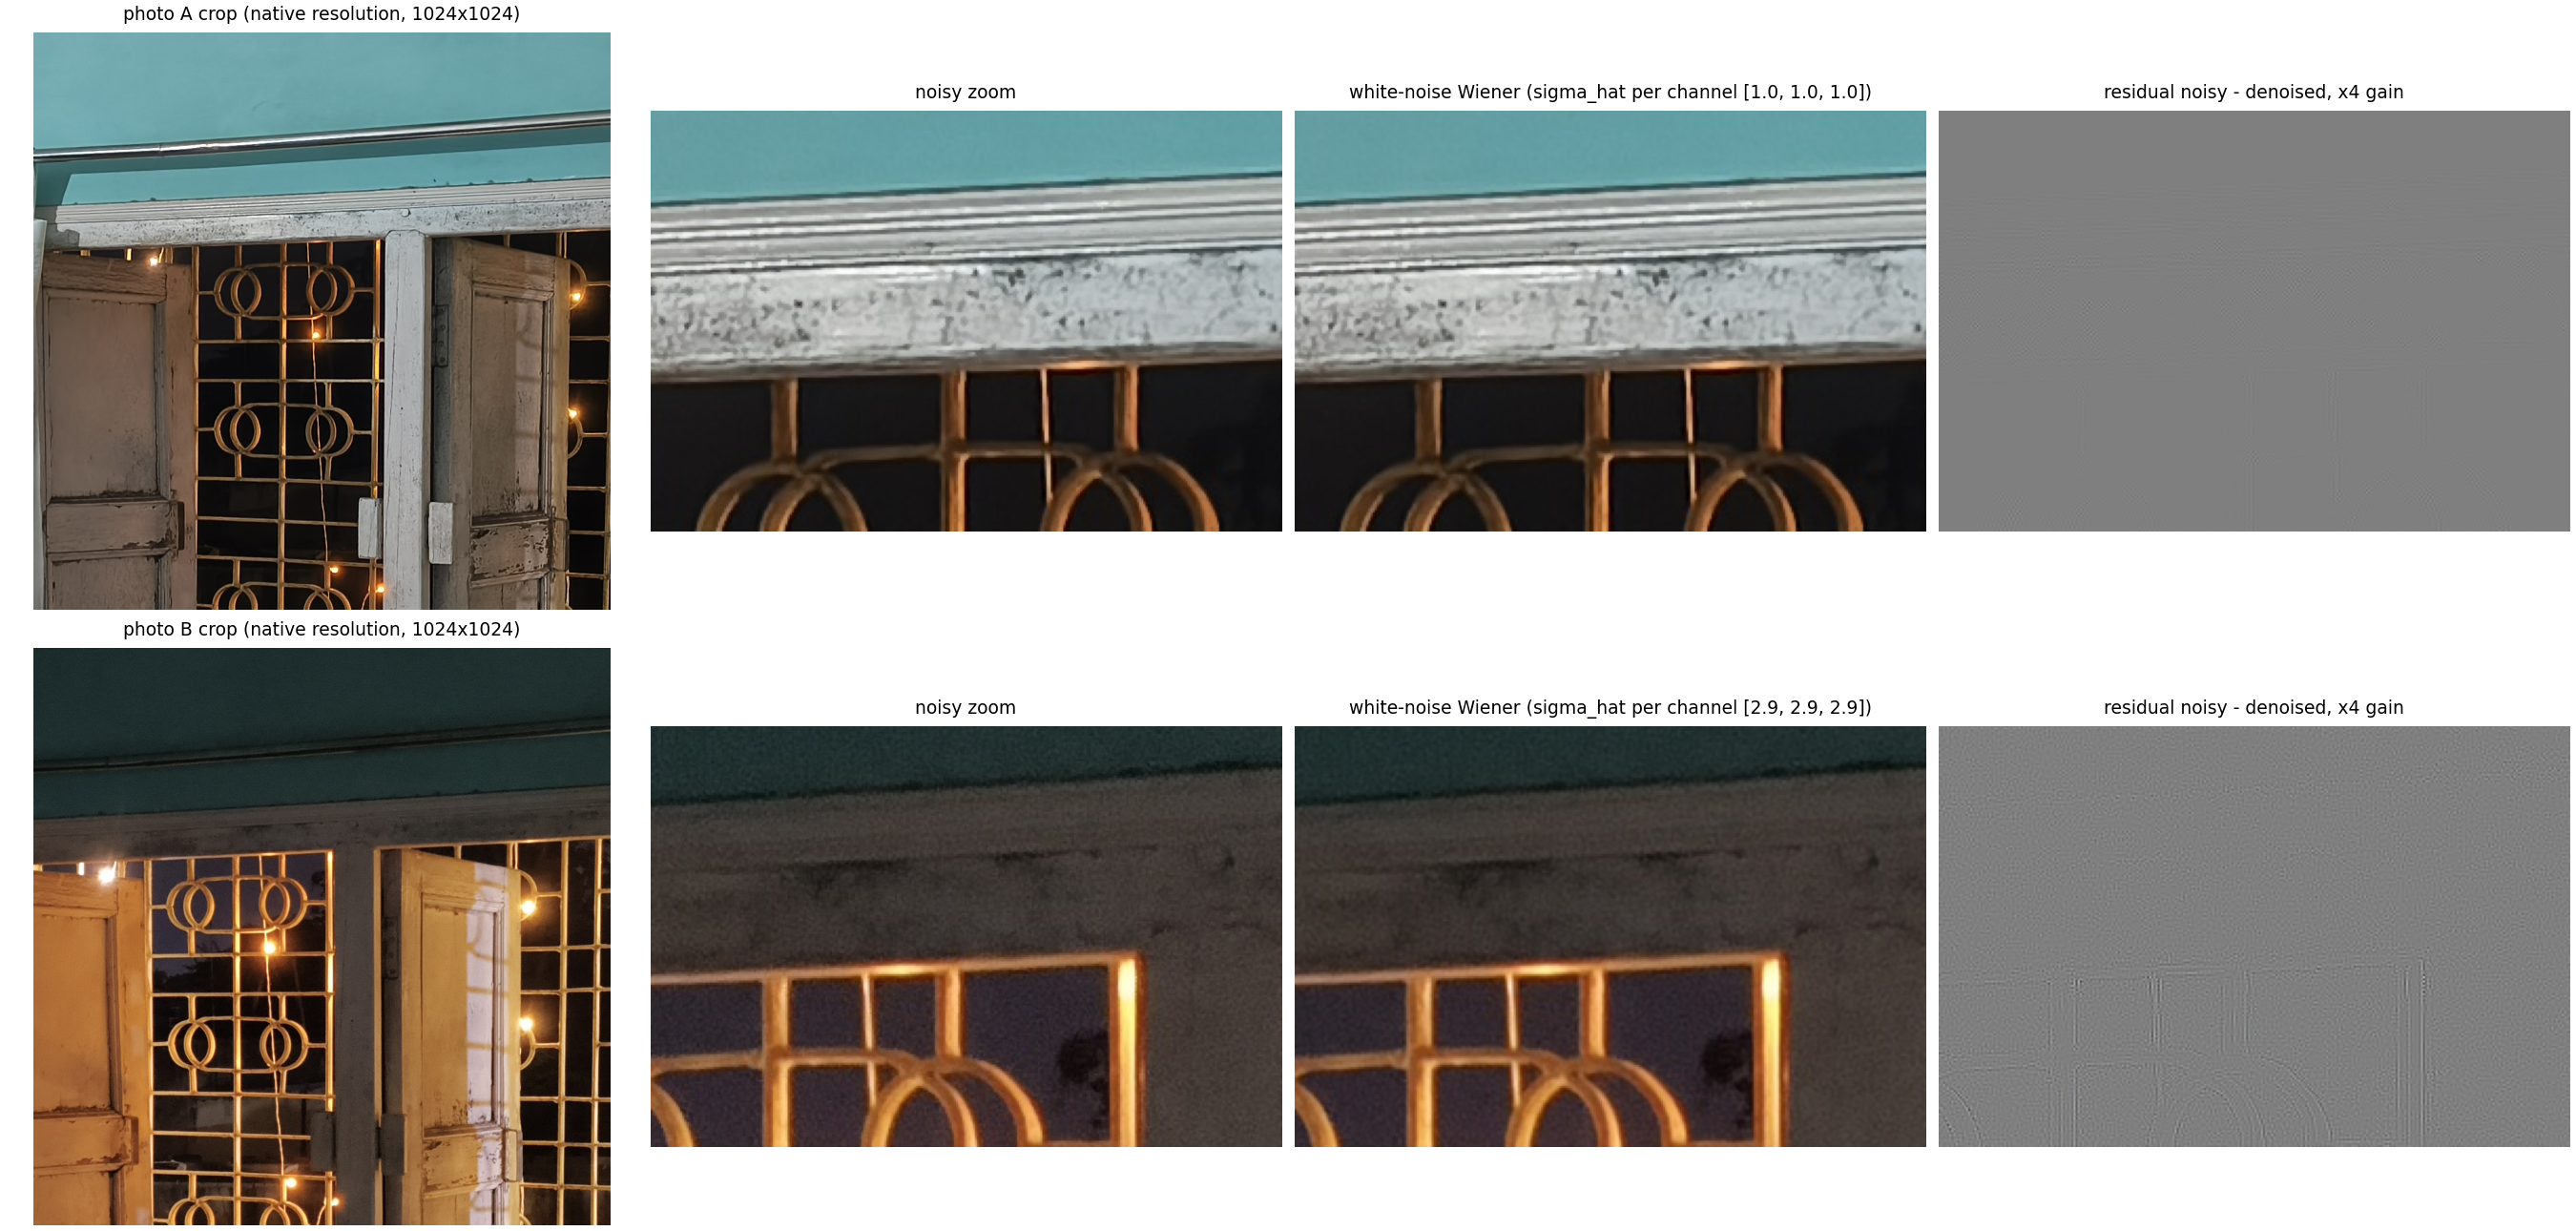
\includegraphics[width=1.00\linewidth]{q5_real_photos}\par\vskip 3pt{\small\textbf{Figure 5.5.} Real photographs at native resolution (A: top, B: bottom). Columns: 1024x1024 crop, noisy zoom, white-noise Wiener output, residual (x4 gain). The residual of B shows edge structure (window frame, arcs): the filter removes signal energy along with noise; the grain that remains in B is blotchy (low-frequency).\par}\end{figure}
\textbf{Qualitative comparison with the synthetic cases and departures from the white-noise model.} In the synthetic cases the noise was white (flat periodogram) and the Wiener output visibly cleaned flat areas while softening edges. On photograph B the denoised crop is only slightly different from the input (mean absolute change 1.14 grey levels; residual standard deviation 1.46/1.70/1.77 in R/G/B, i.e. 51-61\% of the estimated $\hat\sigma$): the grain of B is \textit{not} white. The noise power spectrum of flat patches (Figure 5.4, right, Table 5.5) falls by a factor of 553 between the lowest and the highest radial band (A: 275), versus a flat spectrum for white noise: the noise is dominated by low spatial frequencies (blotches several pixels wide), which is where the signal PSD is large and therefore where the Wiener gain is $\approx1$ - the filter cannot remove it - while the white-noise assumption (flat $S_{nn}$ set to the \textit{total} measured variance) over-attributes power to the high-frequency bands where the true noise power is nearly zero, so there it removes image detail rather than noise (the residual of Figure 5.5 resembles an edge map). Other violations: (i) \textit{signal dependence}: noise grows with brightness (Table 5.4; shot noise is Poisson, $\sigma^2\propto$ signal), so a single $\sigma$ per channel is too large in the shadows and too small near lights; (ii) \textit{demosaicing}: the camera interpolates one colour sample per pixel, which correlates neighbouring pixels and the colour channels (the three channel estimates are nearly equal, which is the signature of processing that treats channels alike); (iii) \textit{in-camera sharpening and denoising}: sharpening boosts mid/high bands and denoising smooths flat areas non-uniformly; (iv) \textit{JPEG compression}: 8x8 block quantisation produces structured, non-Gaussian, spatially correlated errors, strongest in dark flat regions; (v) clipping near the lights. A shot-noise-aware model would use a variance-stabilising transform (Anscombe) before the Wiener filter, and a coloured-noise Wiener filter would use the measured NPS instead of a flat $S_{nn}$.

\begin{table}[H]\centering\scriptsize{\small\textbf{Table 5.5.} Radially averaged noise power spectrum of flat patches (green channel, 52 / 53 patches of 32x32, plane-detrended), 8 equal bands from 0 to 0.5 cycles/pixel, normalised to the mean over bands (white noise would give 1 in every band). Lowest band includes some residual low-frequency scene texture; the strong decay towards high frequency is the evidence of spatially correlated noise.\par}\vskip 3pt
\resizebox{\ifdim\width>\linewidth\linewidth\else\width\fi}{!}{\begin{tabular}{lrrrrrrrr}\toprule
\textbf{photo} & \textbf{band 1} & \textbf{band 2} & \textbf{band 3} & \textbf{band 4} & \textbf{band 5} & \textbf{band 6} & \textbf{band 7} & \textbf{band 8}\\\midrule
A & 5.610 & 1.530 & 0.424 & 0.211 & 0.118 & 0.053 & 0.034 & 0.020\\
B & 6.719 & 0.747 & 0.207 & 0.128 & 0.094 & 0.061 & 0.031 & 0.012\\
\bottomrule\end{tabular}}\end{table}
\section{Question 6 - Motion blur and deblurring}
\subsection{6.1 Model and synthesis}
\textbf{Continuous PSF.} Uniform linear motion of length $L$ along direction $\theta$ during the exposure moves a point of the scene along the segment $t(\cos\theta,\sin\theta)$, $t\in[-L/2,L/2]$, with constant speed, so the energy of a point is spread uniformly along the segment:

\begin{equation}h(x,y)=\frac1L\int_{-L/2}^{L/2}\delta(x-t\cos\theta,\;y-t\sin\theta)\,dt,\qquad \iint h\,dx\,dy=\frac1L\int_{-L/2}^{L/2}dt=1\end{equation}
(a one-dimensional line mass of density $1/L$ per unit length; $x$ is the column direction, $y$ the row direction pointing down, and $\theta$ is measured from $+x$ towards $+y$).

\textbf{Discretisation and normalisation.} The segment is sampled by the midpoint rule at $n=\lceil32L\rceil$ points $t_j=(j+\tfrac12)L/n-L/2$ (each carrying mass $1/n$), and each point is \textit{splatted} with bilinear weights onto the four nearest pixels of a grid with periodic indexing, the origin being pixel $(0,0)$. The result is non-negative, compactly supported (71 non-zero pixels for $L=25$, $\theta=30^\circ$) and sums to exactly 1.0 by construction (also checked in tests). \textbf{Boundary convention (forward and inverse alike): circular}; blurring is $g=\mathcal F^{-1}\{H\,\mathcal F\{f\}\}$ with $H=\mathrm{DFT}\{\text{psf}\}$ on the full image grid and deconvolution divides by the same $H$, so the model used to construct $H$ and the model used to blur are identical (no cropping of boundary pixels is needed). For the real photographs (Section 6.4) the image is mirror-padded before the circular deconvolution to avoid wraparound.

\textbf{Noise and SNR.} The blurred image (in [0,1]) is corrupted by zero-mean white Gaussian noise at a stated SNR, defined as

\begin{equation}\mathrm{SNR}_{dB}=10\log_{10}\frac{\sum_{x,y,c}f(x,y,c)^{2}}{\sum_{x,y,c}n(x,y,c)^{2}},\qquad \sigma_n^{2}=\frac{\sum f^{2}}{N_{px}\,10^{\mathrm{SNR}_{dB}/10}}\end{equation}
with $f$ the \textit{clean} image on the [0,1] scale (not mean-removed). The noise is not clipped. Experiments use the 1536x1024 working version of the instructor-provided reference photograph (Section 5.1; SNR = 20, 30, 40, 50 dB give $\sigma_n=$ 0.0503, 0.0159, 0.0050, 0.0016 on the [0,1] scale).

\textbf{Motion OTF.} Fourier transforming the PSF with $e^{-2\pi i(f_xx+f_yy)}$ (frequencies in cycles/pixel) and using the sifting property,

\begin{equation}H(f_x,f_y)=\frac1L\int_{-L/2}^{L/2}e^{-2\pi i\,t\,s}\,dt=\frac{\sin(\pi L s)}{\pi L s}=\mathrm{sinc}(L s),\qquad s=f_x\cos\theta+f_y\sin\theta\end{equation}
with $\mathrm{sinc}(z)=\sin(\pi z)/(\pi z)$. Zeros occur at $\pi Ls=m\pi$:

\begin{equation}f_x\cos\theta+f_y\sin\theta=\frac{m}{L},\qquad m\in\mathbb Z\setminus\{0\}\end{equation}
\textbf{Adjacent zeros are spaced }$1/L$ in the projected frequency $s$, and each zero set is a \textit{straight line} in the $(f_x,f_y)$ plane with normal vector $(\cos\theta,\sin\theta)$, i.e. \textbf{the zero lines are perpendicular to the motion direction}; $H$ depends on frequency only through its projection on the motion direction, so it is constant along every line perpendicular to the motion, and the dark stripes of $|H|$ are those lines. A discrete FFT grid may sample near, rather than at, the theoretical zeros (the lines do not pass through grid points for general $\theta$).

\textbf{Numerical check of the discretisation.} For the experiment ($L=25$, $\theta=30^\circ$, 1536x1024 grid): $H$ is real to 2.69e-16 (point-symmetric PSF), $H(0,0)=1.0$, and along the motion direction the samples of $|H|$ have their minima at $m/L$ within 3.58e-03 cycles/pixel (largest deviation over the 11 zeros up to 0.45 cycles/pixel; the grid spacing is 1/1536 = 6.5e-4). The DFT of the splatted PSF is \textit{not} exactly the continuous sinc: bilinear splatting convolves the line with the triangle kernel, whose transfer function is $\mathrm{sinc}^2(f_x)\mathrm{sinc}^2(f_y)$, and sampling aliases the product. The relation $H_{DFT}=\sum_{k_x,k_y}\mathrm{sinc}(Ls(f-k))\,\mathrm{sinc}^2(f_x-k_x)\,\mathrm{sinc}^2(f_y-k_y)$ holds to 7.81e-05 over the whole grid (4 aliases each side), and the $k=0$ term alone is accurate to 4.91e-04 for $|f|<0.1$. The extra smooth factor does not move the zero lines. Axis-aligned check: for $L=8$, $\theta=0$ on a 64-point grid $|H|=0e+00, 0e+00, 0e+00$ at $f=m/8$ (m=1,2,3): exact Dirichlet zeros.

\subsection{6.2 Naive inverse filtering and why it fails}
The naive inverse is $\hat F=G/H$ with $G=HF+N$, i.e. $\hat F=F+N/H$. A numerical floor is needed because $H$ has samples at (numerically) zero: $|H|$ is replaced by $\max(|H|,10^{-8})$ keeping its sign (the floor $10^{-8}$ only avoids division by exact zero; a practical floor of $10^{-3}$ is also reported). On the 1536x1024 grid the smallest $|H|$ is 1.71e-08, 18.2\% of the frequency samples have $|H|<10^{-2}$ and 1.72\% have $|H|<10^{-3}$. The noise variance gain $\mathrm{mean}(1/|H|^2)$ is 4.55e+09 with floor $10^{-8}$ and 3.45e+04 with floor $10^{-3}$ (against 1.36e+02 for the Wiener filter with $K=10^{-3}$, Section 6.3).

\begin{figure}[H]\centering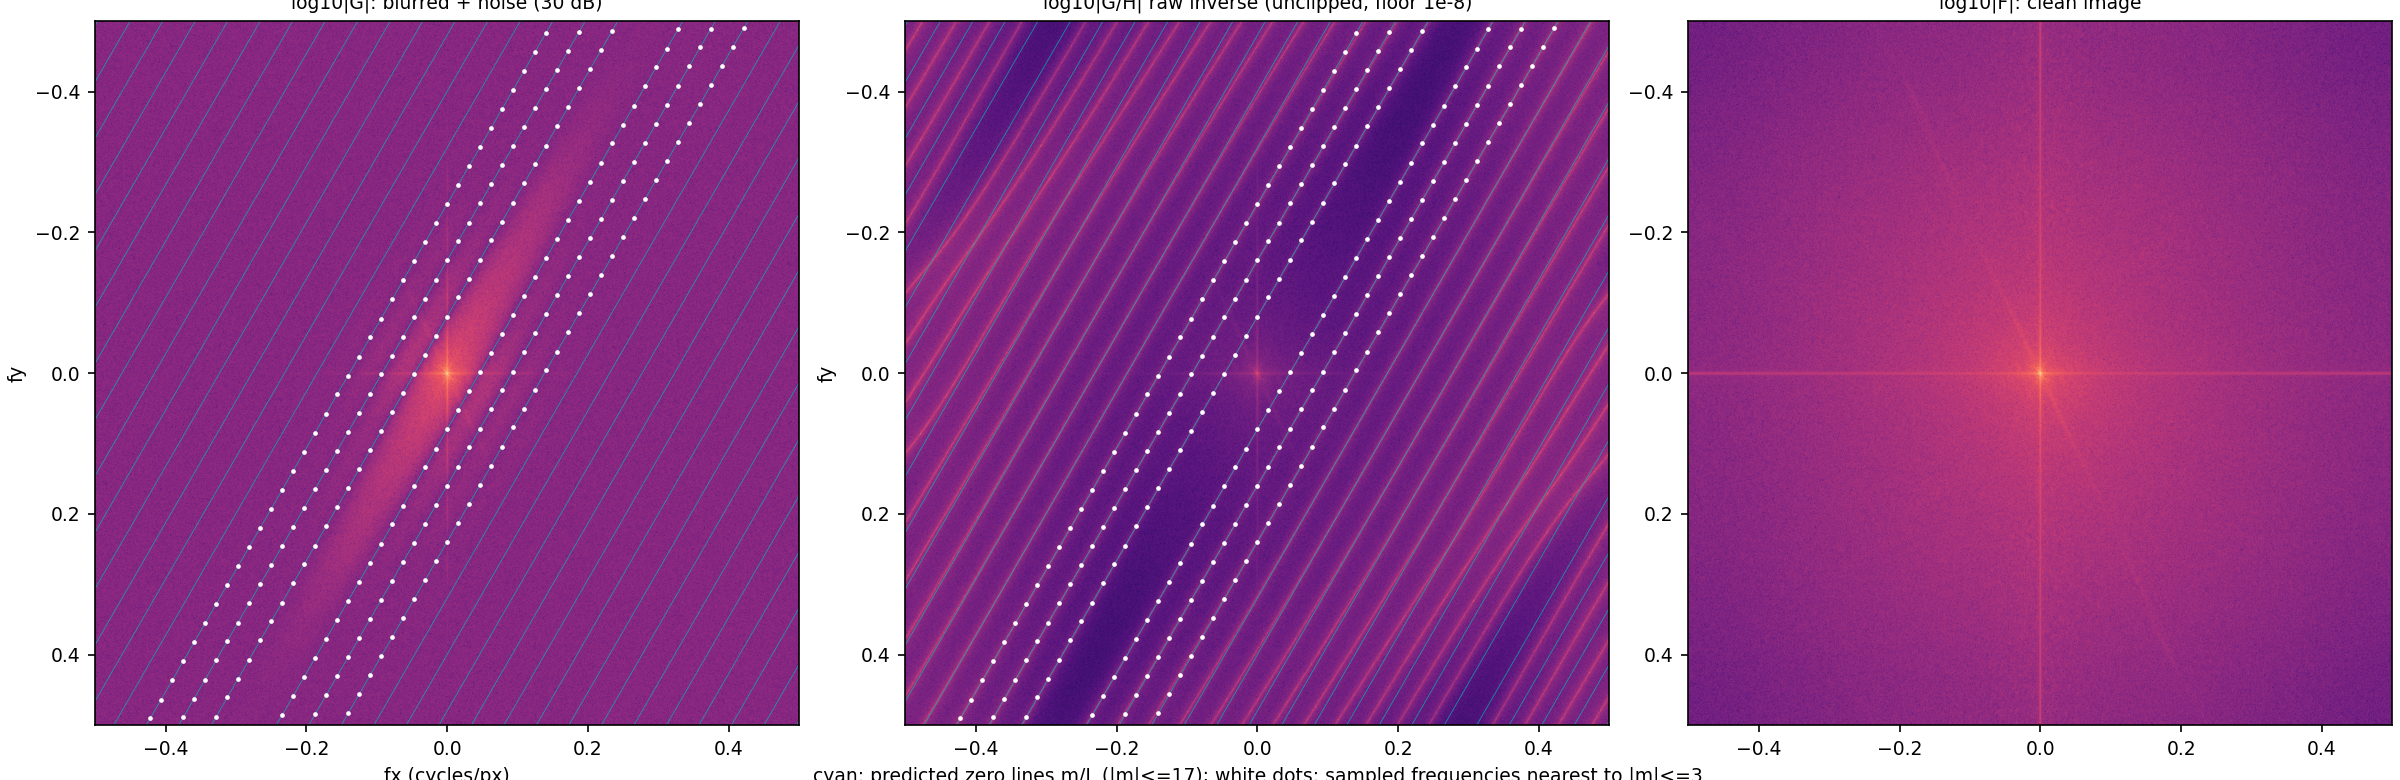
\includegraphics[width=1.00\linewidth]{q6_spectra}\par\vskip 3pt{\small\textbf{Figure 6.1.} Left: log10\textbar{}G\textbar{} of the blurred and noisy (30 dB) luminance. Middle: log10\textbar{}G/H\textbar{}, the raw (unclipped) inverse estimate: the noise is amplified into bright bands exactly on the zero lines of H. Right: log10\textbar{}F\textbar{} of the clean image. Cyan: the predicted zero lines m/L (L = 25, theta = 30 deg, \textbar{}m\textbar{} \textless{}= 17); white dots: the sampled frequencies nearest to the lines m = +-1, +-2, +-3.\par}\end{figure}
\begin{table}[H]\centering\footnotesize{\small\textbf{Table 6.1.} Naive inverse filtering of the blurred+noisy reference image (L=25, theta=30). PSNR (dB, vs the clean image, output clipped for the metric) of the blurred+noisy input and of the inverse estimate with floors 1e-8 and 1e-3; RMS error of the \textit{unclipped} inverse estimate on the [0,1] scale.\par}\vskip 3pt
\resizebox{\ifdim\width>\linewidth\linewidth\else\width\fi}{!}{\begin{tabular}{rrrrrr}\toprule
\textbf{SNR (dB)} & \textbf{achieved SNR} & \textbf{\begin{tabular}[b]{@{}c@{}}PSNR\\{}blurred+noisy\end{tabular}} & \textbf{\begin{tabular}[b]{@{}c@{}}PSNR naive\\{}inverse\\{}(floor 1e-8)\end{tabular}} & \textbf{\begin{tabular}[b]{@{}c@{}}PSNR naive\\{}inverse\\{}(floor 1e-3)\end{tabular}} & \textbf{\begin{tabular}[b]{@{}c@{}}RMS error of\\{}unclipped\\{}inverse\end{tabular}}\\\midrule
20 & 20.000 & 22.09 & 4.46 & 4.67 & 2824\\
30 & 30.000 & 23.91 & 4.46 & 5.14 & 893.2\\
40 & 40.000 & 24.15 & 4.47 & 6.84 & 282.4\\
50 & 50.000 & 24.17 & 4.48 & 12.51 & 89.32\\
\bottomrule\end{tabular}}\end{table}
\textbf{Noise amplification and the zero spacing.} At a frequency where $|H|$ is tiny the term $N/H$ is huge: the amplified-noise bands in Figure 6.1 (middle) are exactly the lines $f_x\cos\theta+f_y\sin\theta=m/L$, repeated with the spacing $1/L=0.04$ cycles/pixel, so a 1536x1024 spectrum is crossed by dozens of such lines and the noise is amplified without bound on each of them. Between the zeros $|H|$ is a sinc side lobe of height $\lesssim1/(\pi L|s|)\approx1/(78|s|)$, so even in the 'pass bands' the inverse multiplies the noise by $1/|H|$, which is large at all but the lowest frequencies. The inverse estimate has an RMS error of 2824 (SNR 20 dB) down to 89.3 (50 dB) on a [0,1] image and PSNR 4.5-4.5 dB, \textit{worse than the blurred input} (22.1-24.2 dB) at all four noise levels.

\textbf{In one sentence:} because the inverse filter multiplies the noise spectrum by $1/H$, any nonzero noise component $N(u,v)$ at a frequency where $|H(u,v)|\to0$ is amplified by the unbounded factor $1/|H(u,v)|$, while the signal $F(u,v)H(u,v)$ there vanishes.

\subsection{6.3 Wiener deconvolution}
\textbf{Derivation.} For $G=HF+N$ with $F$, $N$ uncorrelated with PSDs $S_{ff}$, $S_{nn}$, the linear estimate $\hat F=WG$ minimising $E|F-WG|^2$ at each frequency satisfies the orthogonality condition $E[(F-WG)\bar G]=0$, i.e. $S_{ff}\bar H=W(|H|^2S_{ff}+S_{nn})$, hence

\begin{equation}W(u,v)=\frac{\overline{H}\,S_{ff}}{|H|^{2}S_{ff}+S_{nn}}=\frac{\overline{H}}{|H|^{2}+K},\qquad \hat F=\frac{\overline H\,G}{|H|^{2}+K},\quad K=\frac{S_{nn}}{S_{ff}}\end{equation}
\textbf{Scaling and interpretation of K.} Images are in [0,1] and $H$ has $H(0)=1$; with white noise of variance $\sigma_n^2$ and a signal modelled as a flat spectrum with the \textit{average} signal power $\overline{f^2}=\sum f^2/N_{px}$ (the quantity in the SNR definition), $K=\sigma_n^2/\overline{f^2}=10^{-\mathrm{SNR}_{dB}/10}$: $K$\textbf{ is a constant noise-to-signal power ratio}. For $K\to0$ the filter becomes the inverse $1/H$ (unstable at the zeros); for $|H|^2\ll K$ it becomes $\bar H/K\to0$ (those frequencies are suppressed rather than amplified); for $K\to\infty$ it tends to $\bar H G/K$, i.e. the blurred image blurred \textit{again} by $\bar H$ (under-deconvolution).

\textbf{Sweep.} $K=10^{-8}\ldots10^{0}$ in steps of 0.05 decades (161 values) at each of four noise levels; PSNR is computed against the clean reference for every $K$ (the same noise realisation for all $K$ at a given level). \textbf{Failure modes:} at $K=10^{-8}$ (inverse-like) the PSNR is 4.6, 4.8, 5.6, 8.5 dB for SNR = 20, 30, 40, 50 dB - far below that of the blurred image, because of the amplified noise bands; at $K=1$ the result is under-deconvolved (still blurred, and additionally blurred by $\bar H$) with PSNR 11.8, 11.8, 11.8, 11.8 dB at every noise level (essentially independent of the noise, since the filter has become $\approx\bar H$). The optimum lies between (Figure 6.2, Table 6.2).

\begin{figure}[H]\centering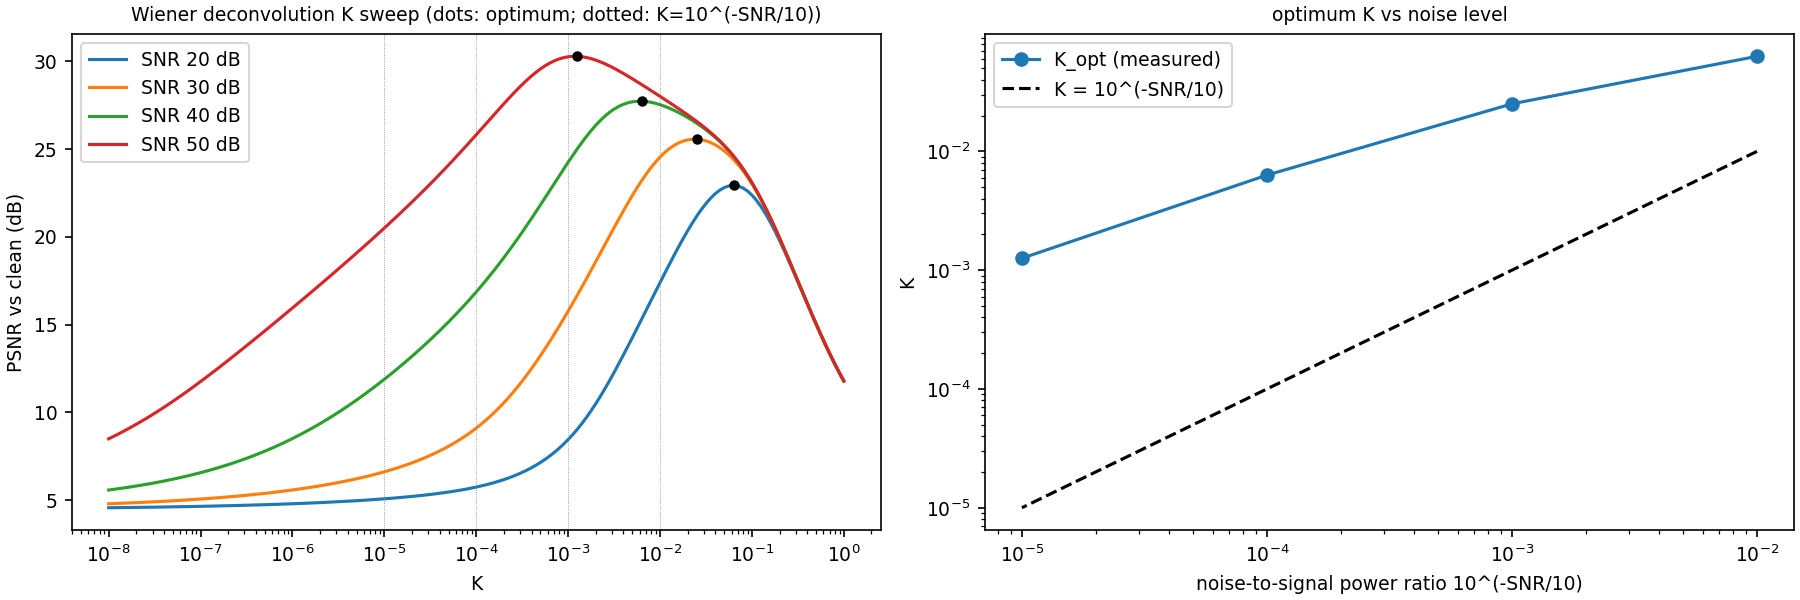
\includegraphics[width=1.00\linewidth]{q6_ksweep}\par\vskip 3pt{\small\textbf{Figure 6.2.} Left: PSNR vs K for four noise levels (black dots: optimum K; dotted vertical lines: the textbook value K = 10\textasciicircum{}(-SNR/10)). Right: measured optimum K against 10\textasciicircum{}(-SNR/10).\par}\end{figure}
\begin{table}[H]\centering\scriptsize{\small\textbf{Table 6.2.} K that maximises PSNR against the clean reference at each noise level (oracle: the clean image is used to read the optimum), compared with the mean-power NSR 10\textasciicircum{}(-SNR/10); PSNR/SSIM at the optimum, PSNR at K = 10\textasciicircum{}(-SNR/10) and of the blurred+noisy input.\par}\vskip 3pt
\resizebox{\ifdim\width>\linewidth\linewidth\else\width\fi}{!}{\begin{tabular}{rrrrrrrr}\toprule
\textbf{SNR (dB)} & \textbf{\begin{tabular}[b]{@{}c@{}}K =\\{}10\textasciicircum{}(-SNR/10)\end{tabular}} & \textbf{\begin{tabular}[b]{@{}c@{}}K\_opt (max\\{}PSNR)\end{tabular}} & \textbf{\begin{tabular}[b]{@{}c@{}}K\_opt /\\{}K\_theory\end{tabular}} & \textbf{\begin{tabular}[b]{@{}c@{}}PSNR at\\{}K\_opt\end{tabular}} & \textbf{\begin{tabular}[b]{@{}c@{}}SSIM at\\{}K\_opt\end{tabular}} & \textbf{\begin{tabular}[b]{@{}c@{}}PSNR at\\{}K\_theory\end{tabular}} & \textbf{\begin{tabular}[b]{@{}c@{}}PSNR\\{}blurred+noisy\end{tabular}}\\\midrule
20 & 0.01 & 0.0631 & 6.3 & 22.93 & 0.376 & 17.39 & 22.09\\
30 & 0.001 & 0.0251 & 25.1 & 25.56 & 0.559 & 15.76 & 23.91\\
40 & 1.0e-04 & 0.00631 & 63.1 & 27.73 & 0.685 & 16.86 & 24.15\\
50 & 1.0e-05 & 0.00126 & 125.9 & 30.28 & 0.793 & 20.50 & 24.17\\
\bottomrule\end{tabular}}\end{table}
\textbf{How the optimum changes with noise level.} $K_{opt}$ decreases monotonically as the noise decreases: 0.0631, 0.0251, 0.00631, 0.00126 for SNR = 20, 30, 40, 50 dB, a factor of 50 over a 1000-fold (30 dB) change in noise power, i.e. $K_{opt}\propto\mathrm{NSR}^{0.57}$ (log-log slope), not proportional to the noise power. It is also larger than the mean-power ratio by a factor of 6.3 to 126, growing as the noise falls. The reason is that $K=S_{nn}/S_{ff}$ assumed one constant $S_{ff}$, whereas natural images have a spectrum falling like $1/f^{\alpha}$: the frequencies where the inverse filter is dangerous (the zeros and the side lobes at higher $|s|$) are mid/high frequencies where $S_{ff}$ is \textit{orders of magnitude below its mean}, so the effective local NSR there is far larger than the global ratio, and the best single constant is a compromise weighted towards them. The gain at the optimum over the blurred+noisy input is 0.8, 1.7, 3.6, 6.1 dB; at $K=K_{theory}$ the result is still dominated by noise bands (PSNR 15.8 dB at 30 dB SNR vs 25.6 dB at $K_{opt}$).

\begin{figure}[H]\centering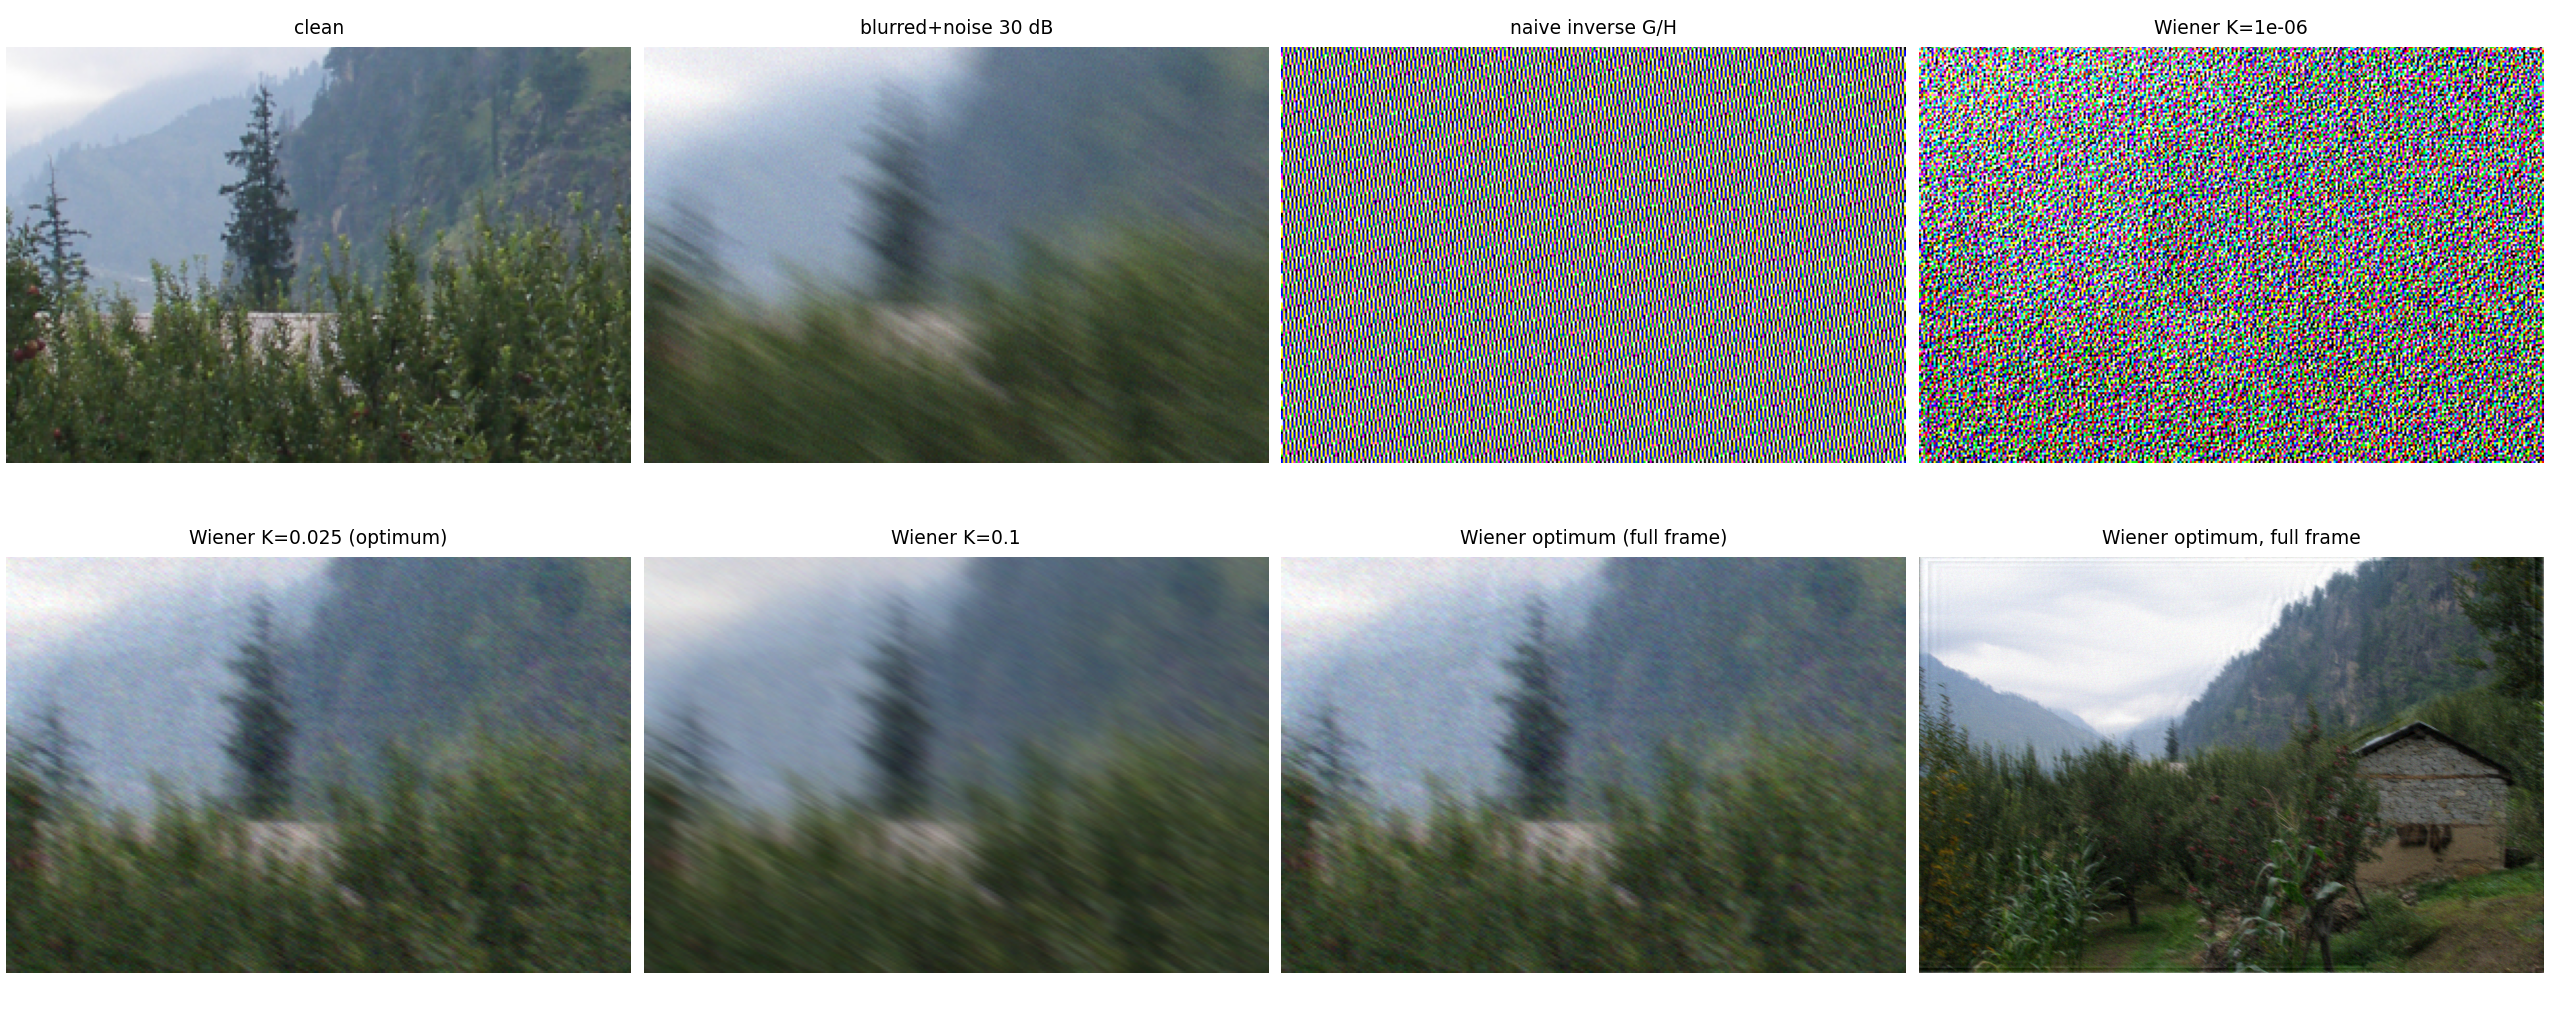
\includegraphics[width=1.00\linewidth]{q6_deconv_grid}\par\vskip 3pt{\small\textbf{Figure 6.3.} Deconvolution at 30 dB SNR (200x300 crop): clean, blurred+noise, naive inverse, Wiener with K = 1e-6 (noise amplification, stripes), K\_opt = 0.025, K = 0.1 (residual blur), and the full-frame optimum.\par}\end{figure}
\subsection{6.4 Estimate the blur from a real photograph, then remove it}
\textbf{Photographs.} Photograph C (\texttt{IMG\_\allowbreak{}20261026\_\allowbreak{}195635983.\allowbreak{}jpg}, 4080x3072, EXIF ISO 491, exposure 1/14 s = 0.07 s, f/1.87, 24 mm-equivalent) is the real motion-blurred photo; photograph D (\texttt{IMG\_\allowbreak{}20261026\_\allowbreak{}195702582.\allowbreak{}jpg}, ISO 722, 1/50 s, same room, different viewpoint) is a sharper photo used only as a \textit{statistical control} in the spectral analysis (never for pixel-wise scores: C and D are not aligned and D is not the sharp version of C). The EXIF data do not record how the camera was held or moved; 1/14 s is much slower than the usual hand-holding guideline of 1/(35 mm-equivalent focal length) = 1/24 s, so camera shake is a plausible cause, but the metadata alone do not establish it. The visible blur is non-uniform (Figures 6.6 and 6.7: the window bars are smeared across tens of pixels, the floor and the door frame much less, the clock face is smeared along a curved path), so a uniform linear model can at best be a first approximation.

\textbf{Estimator 1: single-crop cepstrum + spectral comb (validated on synthetic blur).} For a 1024x1024 grey crop the Hann-windowed power spectrum is divided by its radial mean (whitening). (i) The \textit{cepstrum} of this whitened log-spectrum (inverse FFT, radial trend removed) has a negative peak at the quefrency vector $L(\cos\theta,\sin\theta)$, because $\log\mathrm{sinc}^2(Ls)$ is periodic in $s$ with period $1/L$. (ii) A \textit{comb score} then refines $(L,\theta)$ by minimising the mean whitened log-spectrum on the predicted zero lines $s=m/L$ minus the mean on the half-way lines. The pair was tested on a crop of the sharp photograph D blurred synthetically with known $(L,\theta)$ and without or with noise (2 grey levels): 22 of 26 cases ($L\in\{8,15,25,40,70\}$, angles including 0, 0.7, 89.3, 90, 120, 160 degrees) are recovered within 2 degrees and 10\% (+0.5 px) of the truth; the four exceptions are the three noisy $L=8$ cases (L within 0.8 px, angle off by 3-5 degrees) and the noisy $L=15$, $\theta=89.3^\circ$ case, for which the cepstrum picked a low-quefrency lobe (4.7 px). Table 6.3 lists the validation.

\begin{table}[H]\centering\scriptsize{\small\textbf{Table 6.3.} Single-crop estimator validation: 1024x1024 crop of photograph D blurred synthetically (circular boundary) with known L (px) and theta (deg), without and with additive noise (sigma in grey levels). Cepstrum estimate, comb-refined estimate and the errors of the latter.\par}\vskip 3pt
\resizebox{\ifdim\width>\linewidth\linewidth\else\width\fi}{!}{\begin{tabular}{rrrrrrrrr}\toprule
\textbf{L true} & \textbf{theta true} & \textbf{noise} & \textbf{L cepstrum} & \textbf{\begin{tabular}[b]{@{}c@{}}theta\\{}cepstrum\end{tabular}} & \textbf{L comb} & \textbf{theta comb} & \textbf{theta err} & \textbf{L err}\\\midrule
8 & 0 & 0.0 & 8.0 & 0.1 & 8.0 & 0.1 & 0.1 & 0.01\\
8 & 0 & 2.0 & 8.0 & 7.5 & 7.3 & 5.0 & 5.0 & -0.66\\
8 & 90 & 0.0 & 8.0 & 90.1 & 8.0 & 90.1 & 0.1 & 0.02\\
8 & 90 & 2.0 & 7.9 & 97.9 & 7.2 & 94.9 & 4.9 & -0.77\\
8 & 30 & 0.0 & 8.1 & 29.8 & 8.1 & 29.8 & -0.2 & 0.06\\
8 & 30 & 2.0 & 8.2 & 28.9 & 7.9 & 26.9 & -3.1 & -0.06\\
15 & 30 & 0.0 & 14.8 & 29.7 & 14.8 & 29.7 & -0.3 & -0.22\\
15 & 30 & 2.0 & 15.1 & 30.4 & 14.9 & 30.2 & 0.2 & -0.13\\
15 & 45 & 0.0 & 15.4 & 45.0 & 15.1 & 45.0 & -0.0 & 0.10\\
15 & 45 & 2.0 & 15.0 & 45.8 & 15.0 & 45.8 & 0.8 & 0.01\\
15 & 0.7 & 0.0 & 15.0 & 0.3 & 15.0 & 0.3 & -0.4 & -0.01\\
15 & 0.7 & 2.0 & 15.0 & 3.0 & 14.8 & 0.5 & -0.2 & -0.23\\
15 & 89.3 & 0.0 & 15.0 & 89.9 & 15.0 & 89.9 & 0.6 & -0.01\\
15 & 89.3 & 2.0 & 4.7 & 118.7 & 4.5 & 116.5 & 27.2 & -10.54\\
25 & 30 & 0.0 & 25.4 & 30.4 & 25.1 & 30.1 & 0.1 & 0.10\\
25 & 30 & 2.0 & 24.5 & 30.0 & 24.8 & 30.5 & 0.5 & -0.17\\
25 & 120 & 0.0 & 25.4 & 120.4 & 25.1 & 120.1 & 0.1 & 0.09\\
25 & 120 & 2.0 & 25.4 & 120.1 & 25.1 & 119.8 & -0.2 & 0.12\\
40 & 30 & 0.0 & 40.2 & 29.9 & 40.1 & 29.9 & -0.1 & 0.14\\
40 & 30 & 2.0 & 40.2 & 29.9 & 40.6 & 30.2 & 0.2 & 0.64\\
40 & 160 & 0.0 & 39.4 & 160.1 & 40.0 & 160.1 & 0.1 & -0.00\\
40 & 160 & 2.0 & 40.1 & 160.0 & 40.0 & 160.0 & 0.0 & 0.05\\
70 & 5 & 0.0 & 70.0 & 5.0 & 70.0 & 5.0 & -0.0 & -0.02\\
70 & 5 & 2.0 & 69.7 & 4.9 & 69.7 & 4.9 & -0.1 & -0.27\\
70 & 100 & 0.0 & 70.0 & 99.9 & 70.0 & 99.9 & -0.1 & 0.01\\
70 & 100 & 2.0 & 69.9 & 99.9 & 70.9 & 99.9 & -0.1 & 0.92\\
\bottomrule\end{tabular}}\end{table}
\begin{table}[H]\centering\scriptsize{\small\textbf{Table 6.4.} Single-crop estimator applied to native-resolution 1024x1024 crops of the real photographs (origins row,col). 'z (peak)' = z-score of the cepstral peak against its annulus; 'z (comb)' = comb score relative to 300 random (theta, L) draws: \textbar{}z\textbar{} \textless{} 3 means no stripe pattern.\par}\vskip 3pt
\resizebox{\ifdim\width>\linewidth\linewidth\else\width\fi}{!}{\begin{tabular}{llrrrrrrr}\toprule
\textbf{photo} & \textbf{crop} & \textbf{origin} & \textbf{L cepstrum} & \textbf{\begin{tabular}[b]{@{}c@{}}theta\\{}cepstrum\end{tabular}} & \textbf{z (peak)} & \textbf{L comb} & \textbf{theta comb} & \textbf{z (comb)}\\\midrule
C & window & 850,100 & 4.6 & 150.0 & -20.6 & 4.9 & 153.0 & 0.4\\
C & door & 700,1900 & 4.6 & 117.7 & -16.3 & 4.9 & 117.4 & -0.7\\
C & floor & 1700,1500 & 4.5 & 62.9 & -27.4 & 4.9 & 65.6 & -1.0\\
C & wall\_clock & 200,1000 & 4.6 & 152.9 & -26.7 & 4.9 & 155.9 & 0.4\\
D & window & 850,100 & 4.5 & 60.4 & -19.1 & 4.3 & 63.4 & -0.3\\
D & door & 700,1900 & 4.5 & 25.0 & -19.4 & 4.3 & 22.0 & -0.9\\
D & floor & 1700,1500 & 4.5 & 62.2 & -16.9 & 4.3 & 65.2 & -0.3\\
D & wall\_clock & 200,1000 & 6.4 & 49.2 & -21.6 & 6.0 & 46.4 & -1.9\\
\bottomrule\end{tabular}}\end{table}
\textbf{Result on the real photographs: no clean zero-line pattern.} On every crop of C and of the control D the cepstral peak lies at 4.5-6.4 px, at the lower edge of the search interval [4, 150], with the same behaviour on the sharp photograph D (and on the \textit{unblurred} test crop itself the cepstrum reports a peak of z = -11.4 at L = 5.3 px: a large cepstral z-score is not evidence of blur, it is the low-quefrency lobe of the scene's own spectral envelope); the comb scores relative to random $(\theta,L)$ are indistinguishable from chance ($|z|\le1.9$). The single-crop spectra (Figure 6.4, bottom right) show the strong axis-aligned structure of the scene (bright vertical and horizontal bands) but \textbf{no periodic dark stripes}. This is the limitation the assignment anticipates: for real camera-shake blur the zero lines are not observable in a single crop, because (i) the blur is spatially non-uniform (different blur lengths in different parts of the crop average the sinc$^2$ pattern into a smooth decay), (ii) the scene's own spectrum and the noise/JPEG floor mask the side lobes, and (iii) the crop contains edges of all orientations. \textbf{A stripe pattern is therefore not forced from this estimator; its output is not used.}

\textbf{Estimator 2: tile-averaged, control-normalised spectral analysis (adopted).} Averaging the whitened log-spectrum over many different 512x512 tiles of the whole frame (35 tiles per photograph) cancels the scene content of each tile but keeps what is common: the blur and the global scene statistics (a room full of straight horizontal/vertical edges). The remaining scene anisotropy is cancelled with the tile-averaged spectrum of the sharper photograph D as a \textit{control} (same room, same kind of content; a statement about spectral statistics, not a pixel-level reference). (a) \textit{Direction:} blur along $\theta$ removes energy at frequencies along $\theta$; after whitening, the difference of the angular profiles of $S_C-S_D$ in the band 0.02-0.12 cycles/pixel is therefore \textit{maximal perpendicular to the blur}; its maximum is at 93.8 degrees (Figure 6.4, top middle), giving $\hat\theta=3.8^\circ$ (nearly horizontal motion). The difference ranges from -2.21 (along $\theta\approx0$: energy removed) to +1.23 (at 90 degrees). (b) \textit{Length:} the double ratio $Q(f)=[S_C(f,\hat\theta)-S_C(f,\hat\theta+90^\circ)]-[S_D(f,\hat\theta)-S_D(f,\hat\theta+90^\circ)]$ estimates $\log|H(f)|^2$ along the blur direction with the scene anisotropy cancelled. It falls from -0.45 at 0.012 cycles/pixel to -2.39 at 0.042 and then stays near a floor of about -2.96 up to 0.15 cycles/pixel. The sharp periodic dips of a uniform box blur are replaced by weak undulations: the stripe contrast (value of $Q$ at $m/\hat L$ minus the mean at the two half-way points; negative = dip) is -1.28, -0.47, -0.24, 0.35, -0.07 for $m=1\ldots5$ against -1.79, -0.77, -0.42, -0.26, -0.17 for the box model, i.e. dips of the right sign at $m=1,2,3$ but only a fraction of the expected depth, so the stripes beyond the first are smeared. Only the first lobe is quantitatively informative; fitting $\log[(\mathrm{sinc}^2(Lf)+\kappa)/(1+\kappa)]$ ($\kappa=0.02$ allows a floor) over $f\le0.05$ gives $\hat L=33.0$\textbf{ px} (fit error within 25\% of its minimum for $L\in[32.0,34.5]$). The first zero at $1/\hat L=0.0303$ cycles/pixel is therefore the \textit{estimated} spacing of the stripes; it is marked in Figure 6.4 (cyan lines at $m/\hat L$, spacing 0.0303 cycles/pixel) but only the first stripe is clearly supported by the data (the later ones only weakly).

\begin{table}[H]\centering\footnotesize{\small\textbf{Table 6.5.} Validation of estimator 2 on synthetic blur: the 35 tiles of photograph D are split into two disjoint sets; one set is blurred with known (L, theta) and its tile-averaged spectrum is compared with the other, unblurred half as control. The L = 40, theta = 90 case is not identified: its first zero (0.025 cycles/pixel) lies near the lower end of the fit band and the fit-error minimum is flat up to L = 100 (range column).\par}\vskip 3pt
\resizebox{\ifdim\width>\linewidth\linewidth\else\width\fi}{!}{\begin{tabular}{rrrrrrr}\toprule
\textbf{L true} & \textbf{theta true} & \textbf{theta est} & \textbf{\begin{tabular}[b]{@{}c@{}}theta err\\{}(deg)\end{tabular}} & \textbf{L est} & \textbf{\begin{tabular}[b]{@{}c@{}}L range (fit\\{}error \textless{}=\\{}1.25 min)\end{tabular}} & \textbf{L err \%}\\\midrule
30 & 2 & 2.2 & 0.2 & 29.5 & 27.5-31.0 & -1.7\\
30 & 45 & 43.6 & -1.4 & 29.5 & 27.5-32.0 & -1.7\\
20 & 0 & 176.4 & -3.6 & 19.0 & 17.5-20.5 & -5.0\\
40 & 90 & 91.0 & 1.0 & 100.0 & 39.5-100.0 & 150.0\\
30 & 150 & 148.1 & -1.9 & 29.5 & 28.0-31.0 & -1.7\\
\bottomrule\end{tabular}}\end{table}
\begin{figure}[H]\centering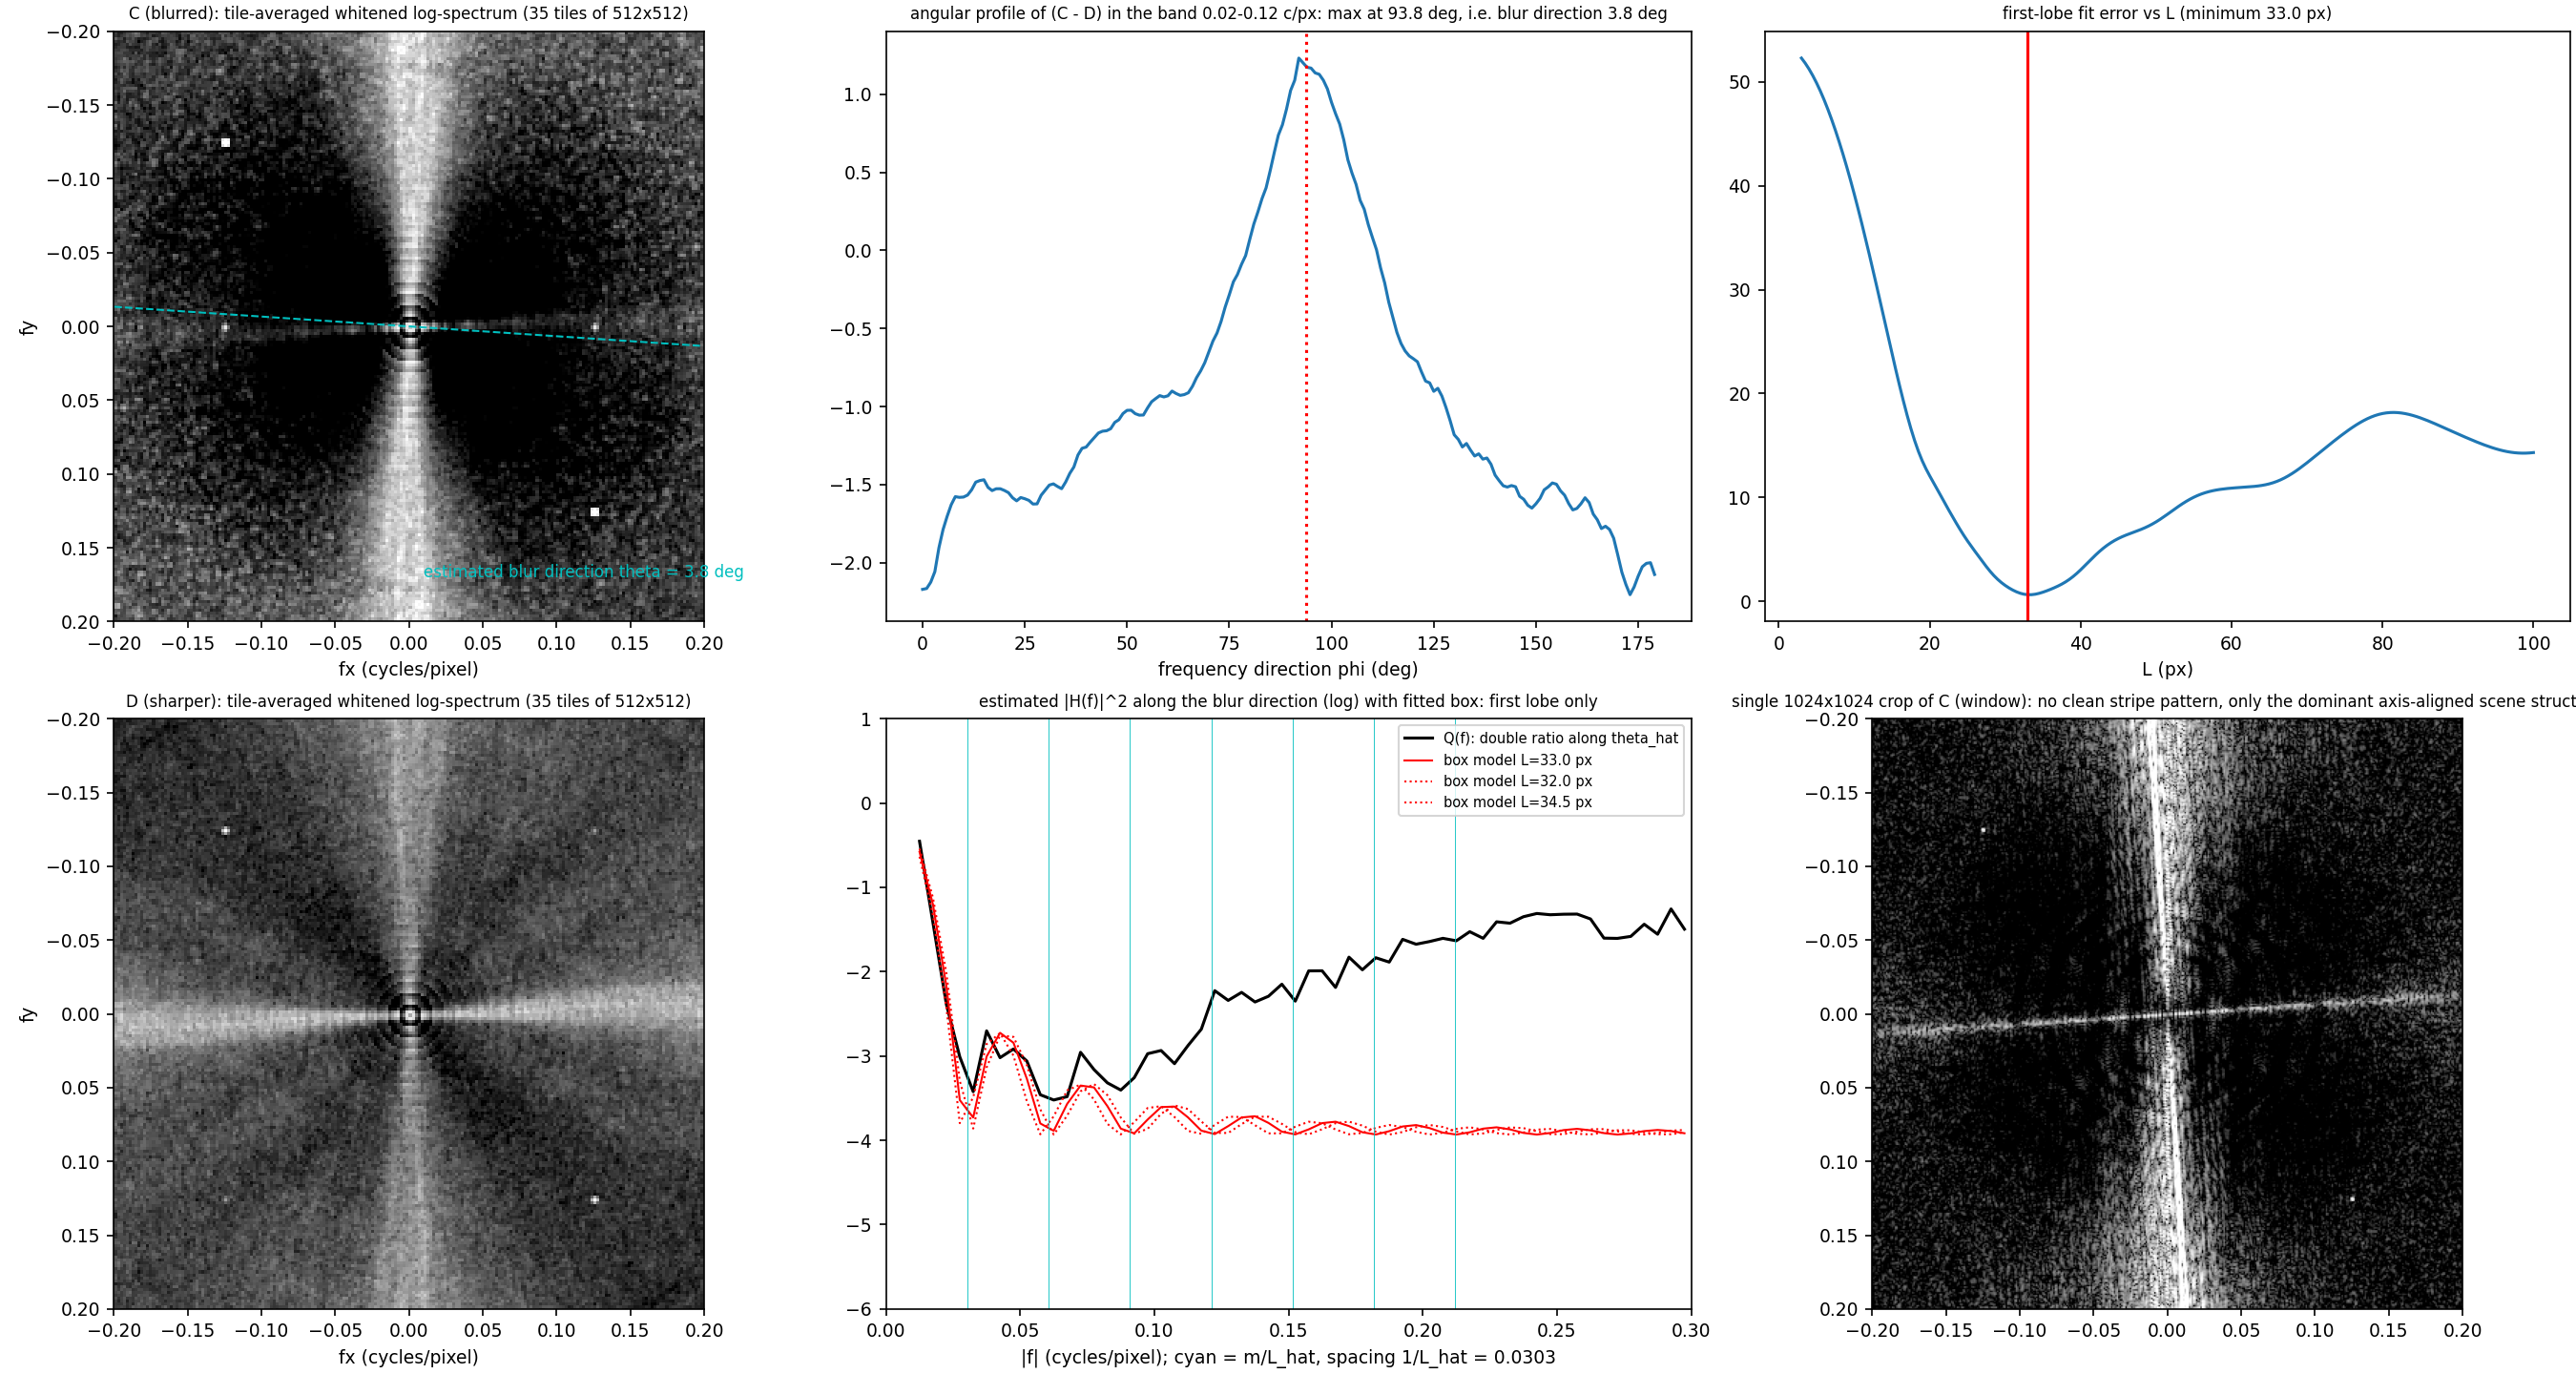
\includegraphics[width=1.00\linewidth]{q6_real_spectra}\par\vskip 3pt{\small\textbf{Figure 6.4.} Real photographs. Top left: tile-averaged whitened log-spectrum of C (35 tiles of 512x512) with the estimated blur direction (cyan dashed); top middle: angular profile of C - D in the 0.02-0.12 c/px band (maximum perpendicular to the blur); top right: first-lobe fit error vs L. Bottom left: tile-averaged spectrum of the sharper D (energy along the horizontal frequency axis retained); bottom middle: double ratio Q(f) = log\textbar{}H\textbar{}\textasciicircum{}2 along the blur direction with the box model (cyan lines at m/L-hat); bottom right: a single 1024x1024 crop of C: no stripe pattern.\par}\end{figure}
\begin{figure}[H]\centering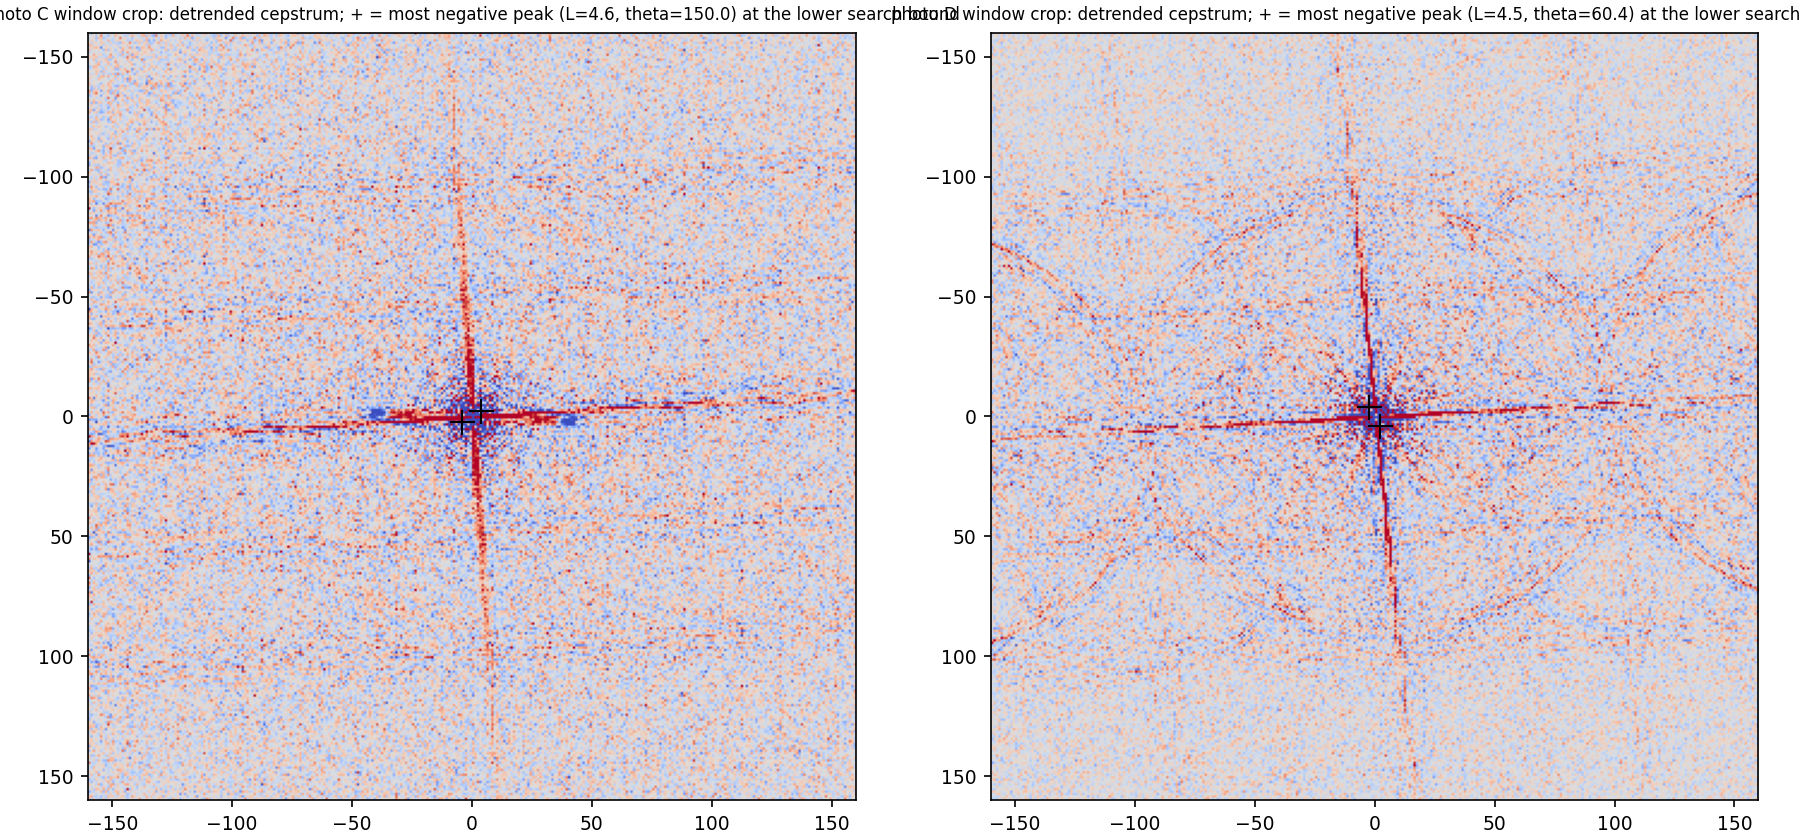
\includegraphics[width=0.75\linewidth]{q6_real_cepstrum}\par\vskip 3pt{\small\textbf{Figure 6.5.} Cepstra of the single window crops of C and D: the most negative peak (+) lies near the origin for both photographs (not a blur signature).\par}\end{figure}
\textbf{Why the dark stripes are perpendicular to the motion.} $H$ depends on $(f_x,f_y)$ only through $s=f_x\cos\theta+f_y\sin\theta$, the component of the frequency vector along the motion; $|H|=|\mathrm{sinc}(Ls)|$ is therefore constant on lines $s=\mathrm{const}$, which are perpendicular to $(\cos\theta,\sin\theta)$, and vanishes on the lines $s=m/L$. A blur along $x$ ($\theta\approx0$) produces vertical stripes in the spectrum; equivalently the image keeps its contrast for structures varying along $y$ (horizontal edges: spectral energy on the vertical frequency axis, preserved in C) and loses it for structures varying along $x$ (vertical bars: spectral energy on the horizontal frequency axis, suppressed in C by about 2 natural-log units relative to D).

\subsubsection{Deblurring with the estimated PSF}
\textbf{Estimated parameters.} \textit{Automatic estimate} (estimator 2, unchanged): $\hat\theta=3.8^\circ$, $\hat L=33.0$ px. \textbf{Adopted} PSF: the same values, no manual adjustment. For $K$ the noise level of the crop was measured from flat patches ($\hat\sigma_{RGB}=1.57, 1.50, 1.34$ grey levels) and the signal variance of the crop is 1801, 1720, 1175 (RGB), so the constant noise-to-signal ratio is $K_{est}=\overline{\hat\sigma^2/\mathrm{var}}=1.41e-03$. Because the PSF is only approximately right, $K_{est}$ (derived from noise alone) is too small: Figure 6.6 shows $K=0.1,1,10,100,1000\times K_{est}$ and Table 6.6 the fraction of output pixels outside [0,255] (a diagnostic of ringing and noise amplification, \textbf{not a quality score}). \textbf{Adopted }$K=1.41e-02=10\,K_{est}$, chosen by inspection of the sweep as the compromise between sharpening and noise/ringing; no ground truth exists and this is a judgement.

\begin{table}[H]\centering\footnotesize{\small\textbf{Table 6.6.} Wiener deconvolution of the 1024x1024 window crop of photograph C with L = 33.0 px, theta = 3.8 deg: diagnostics of the output for five values of K (no reference exists: these are not PSNR/SSIM).\par}\vskip 3pt
\resizebox{\ifdim\width>\linewidth\linewidth\else\width\fi}{!}{\begin{tabular}{rrrrrr}\toprule
\textbf{K / K\_est} & \textbf{K} & \textbf{\begin{tabular}[b]{@{}c@{}}\% pixels\\{}outside\\{}[0,255]\end{tabular}} & \textbf{min} & \textbf{max} & \textbf{\begin{tabular}[b]{@{}c@{}}RMS change\\{}vs blurred\\{}input\end{tabular}}\\\midrule
0.1 & 1.41e-04 & 26.8 & -348 & 498 & 59.8\\
1 & 1.41e-03 & 18.7 & -217 & 357 & 32.3\\
10 & 1.41e-02 & 9.3 & -96 & 251 & 15.0\\
100 & 1.41e-01 & 5.9 & -28 & 181 & 6.9\\
1e+03 & 1.41e+00 & 3.6 & -3 & 82 & 23.7\\
\bottomrule\end{tabular}}\end{table}
\begin{figure}[H]\centering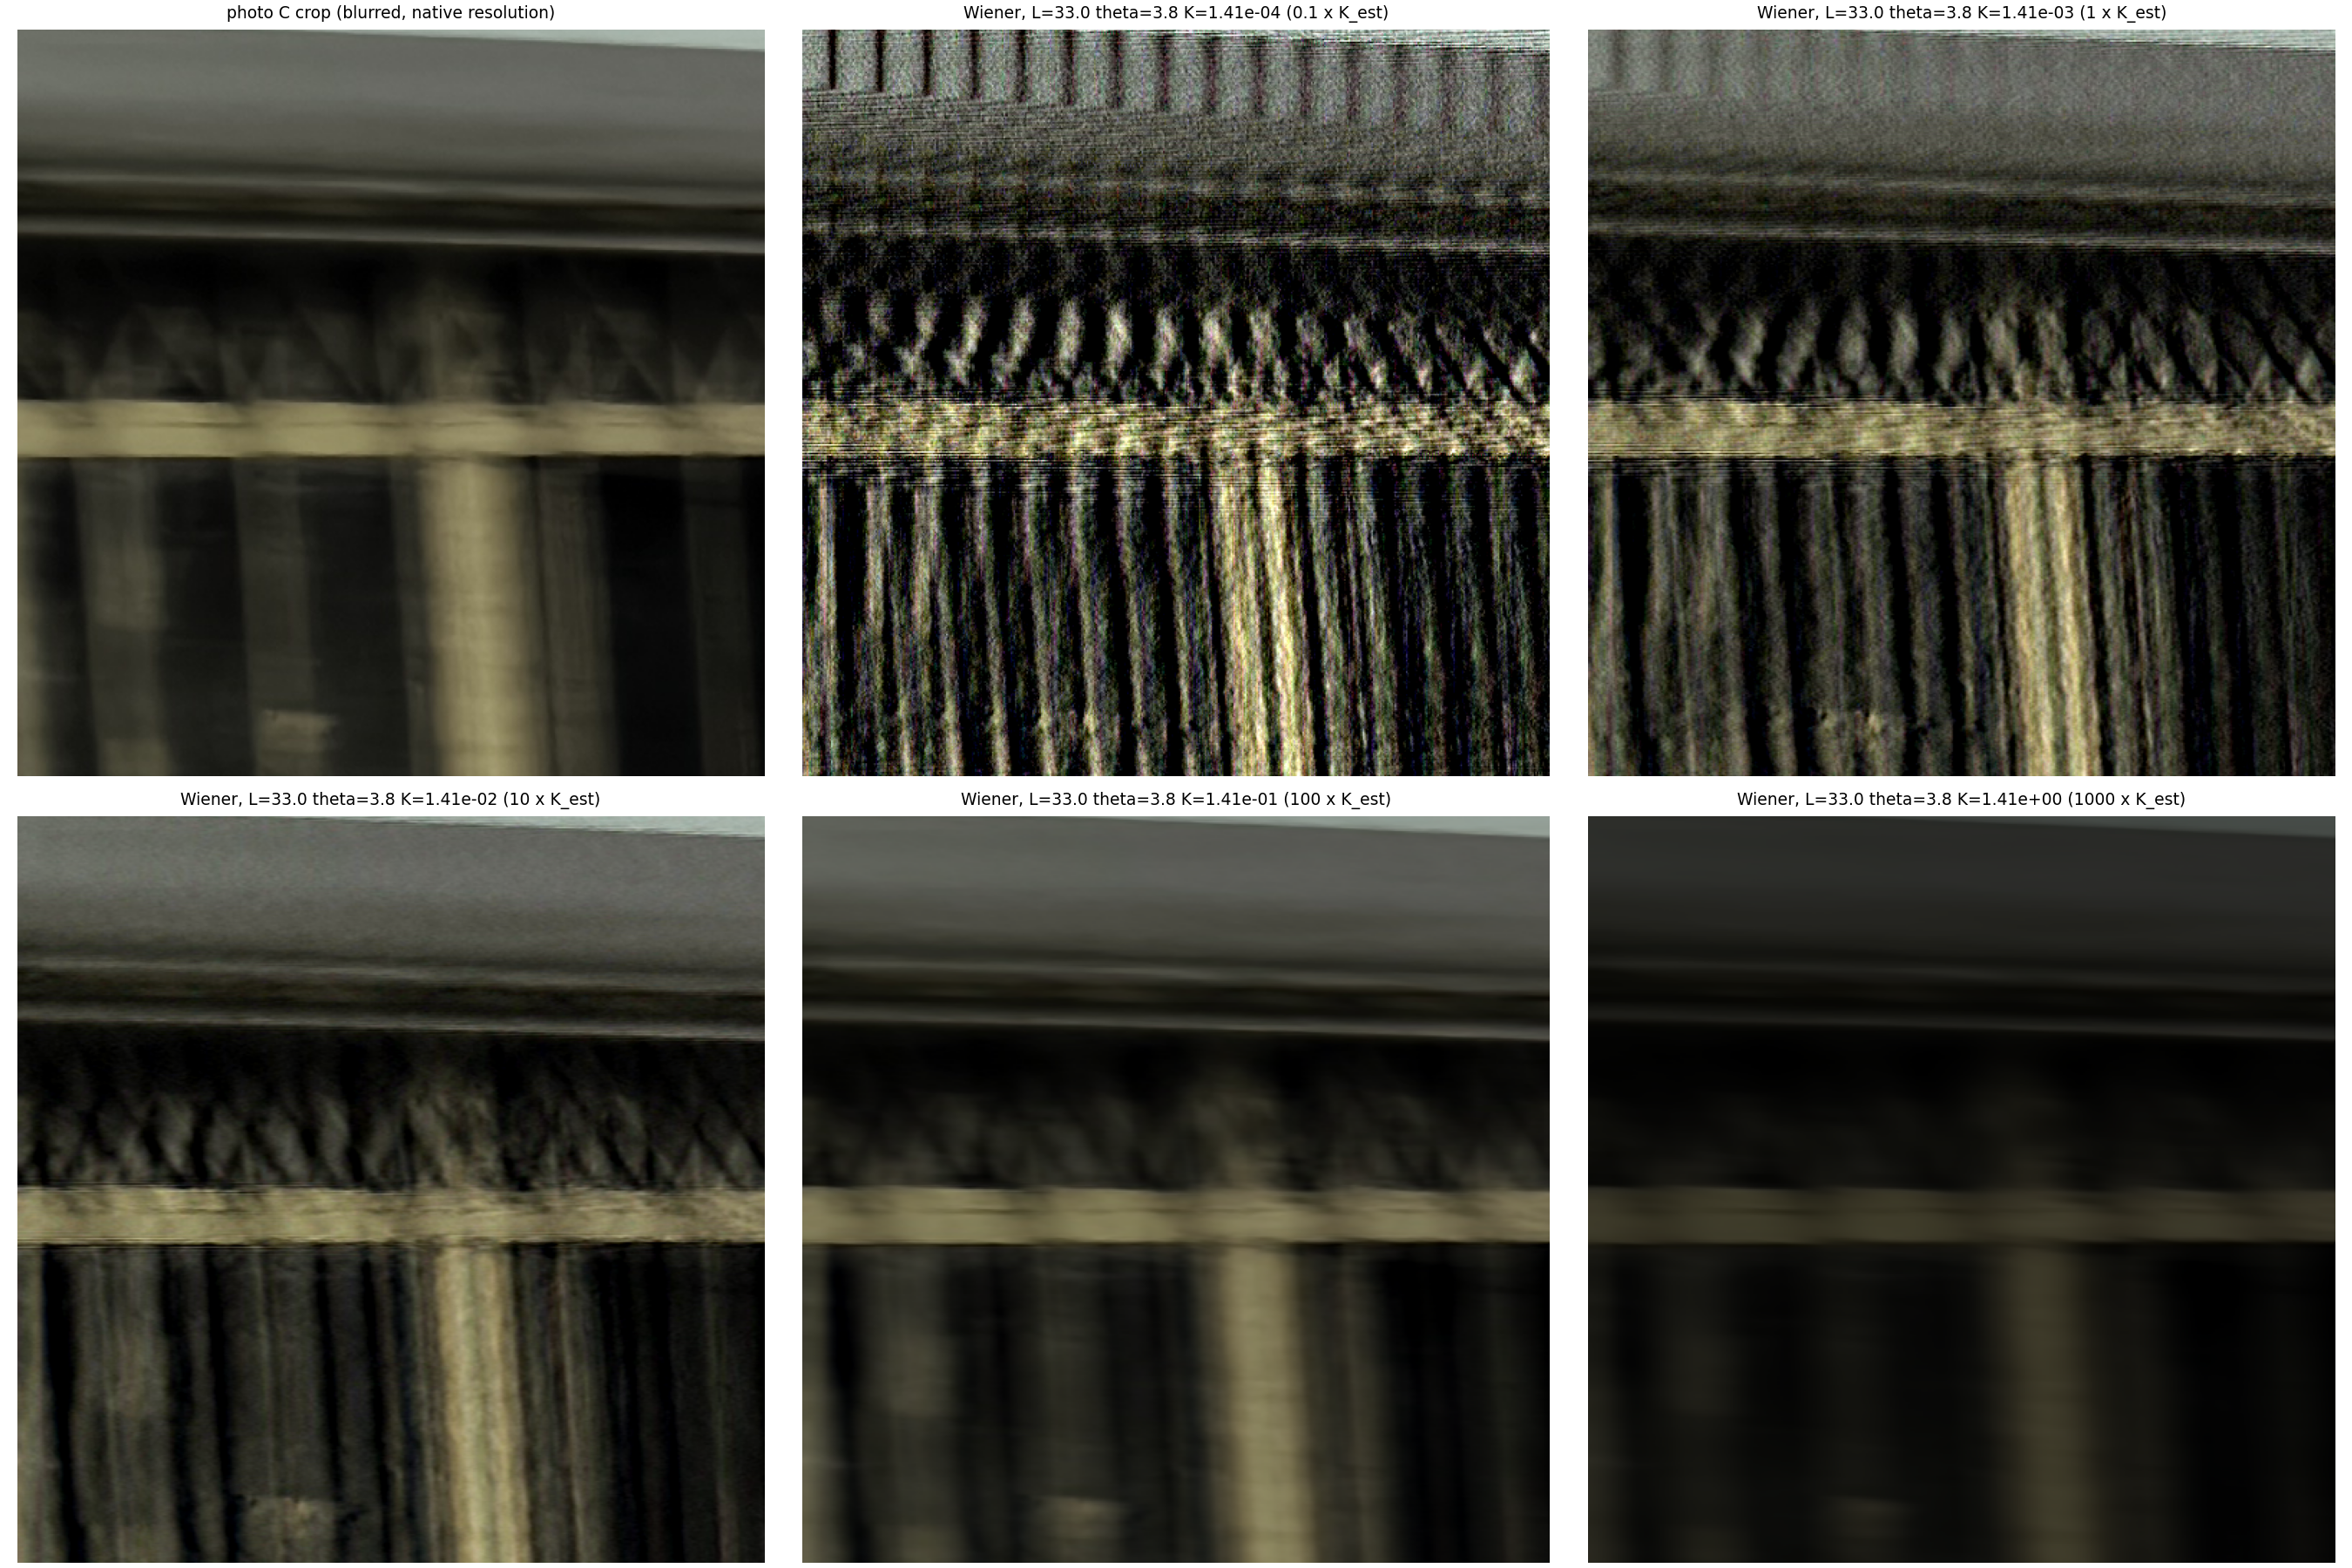
\includegraphics[width=1.00\linewidth]{q6_real_deblur}\par\vskip 3pt{\small\textbf{Figure 6.6.} Photograph C, window crop (native resolution, top-left 520x520 shown): blurred input and Wiener deconvolution with the estimated PSF for K = 0.1, 1, 10, 100, 1000 x K\_est. The vertical bars and the ornament separate clearly at 1-10 x K\_est; large K under-deconvolves.\par}\end{figure}
\begin{figure}[H]\centering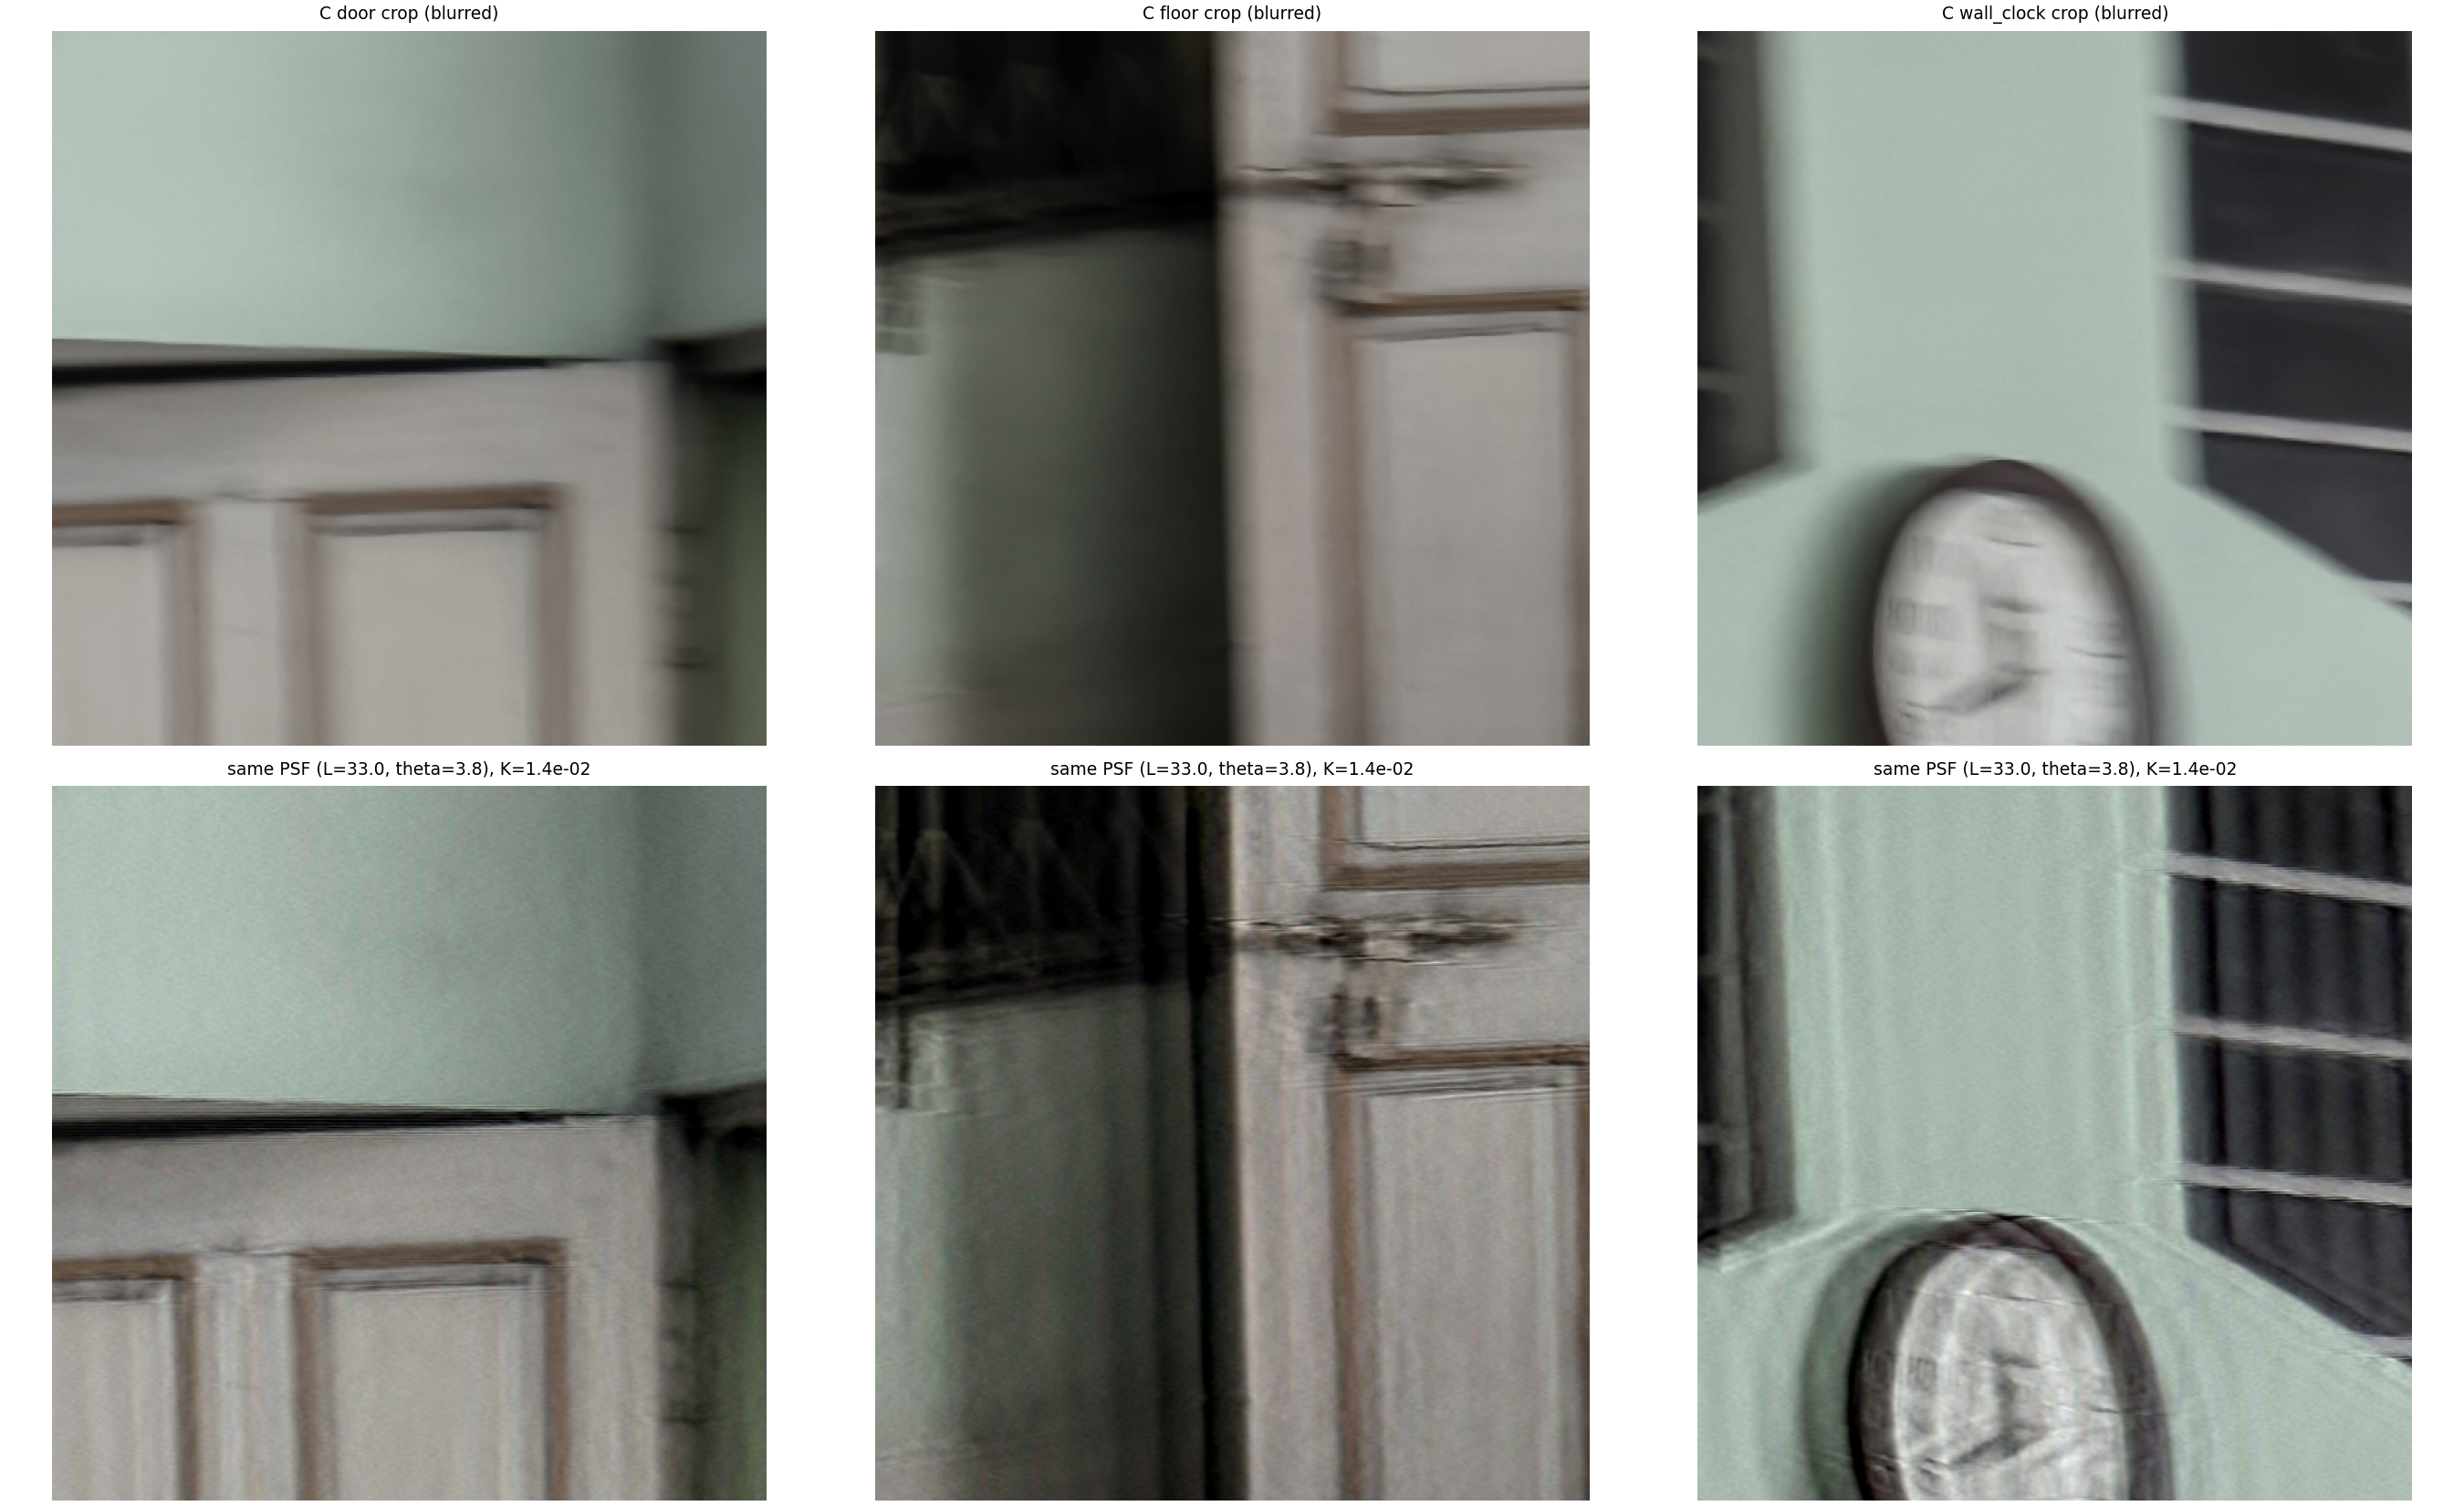
\includegraphics[width=1.00\linewidth]{q6_real_other_crops}\par\vskip 3pt{\small\textbf{Figure 6.7.} The same global PSF (L = 33, theta = 3.8, adopted K) applied to three other crops of C (door, door frame/floor, wall clock): panel edges and the clock face are recovered, but ringing and curved double contours remain where the true blur differs from the global estimate (clock outline, left of the floor crop).\par}\end{figure}
\textbf{Qualitative evaluation (no ground truth, no PSNR/SSIM).} The deconvolution recovers detail that is invisible in the input: the window bars (thin dark gaps between narrow vertical bars) and the ornamental triangles, the door panel edges and mouldings, and the clock hands and numerals partially. Smaller $K$ gives sharper but noisier results with horizontal streaks (noise amplification where $|H|$ is small, Section 6.2); larger $K$ keeps the blur (the under-deconvolution of Section 6.3): at $1000K_{est}$ the output is essentially the dimmed, still-blurred image. As a control, deconvolving the sharper photograph D (which is not blurred along this direction) with the same PSF (Figure 6.8) produces ringing and over-sharpening instead of new detail, so what is recovered in C is real blur removal and not an artefact of the filter.

\begin{figure}[H]\centering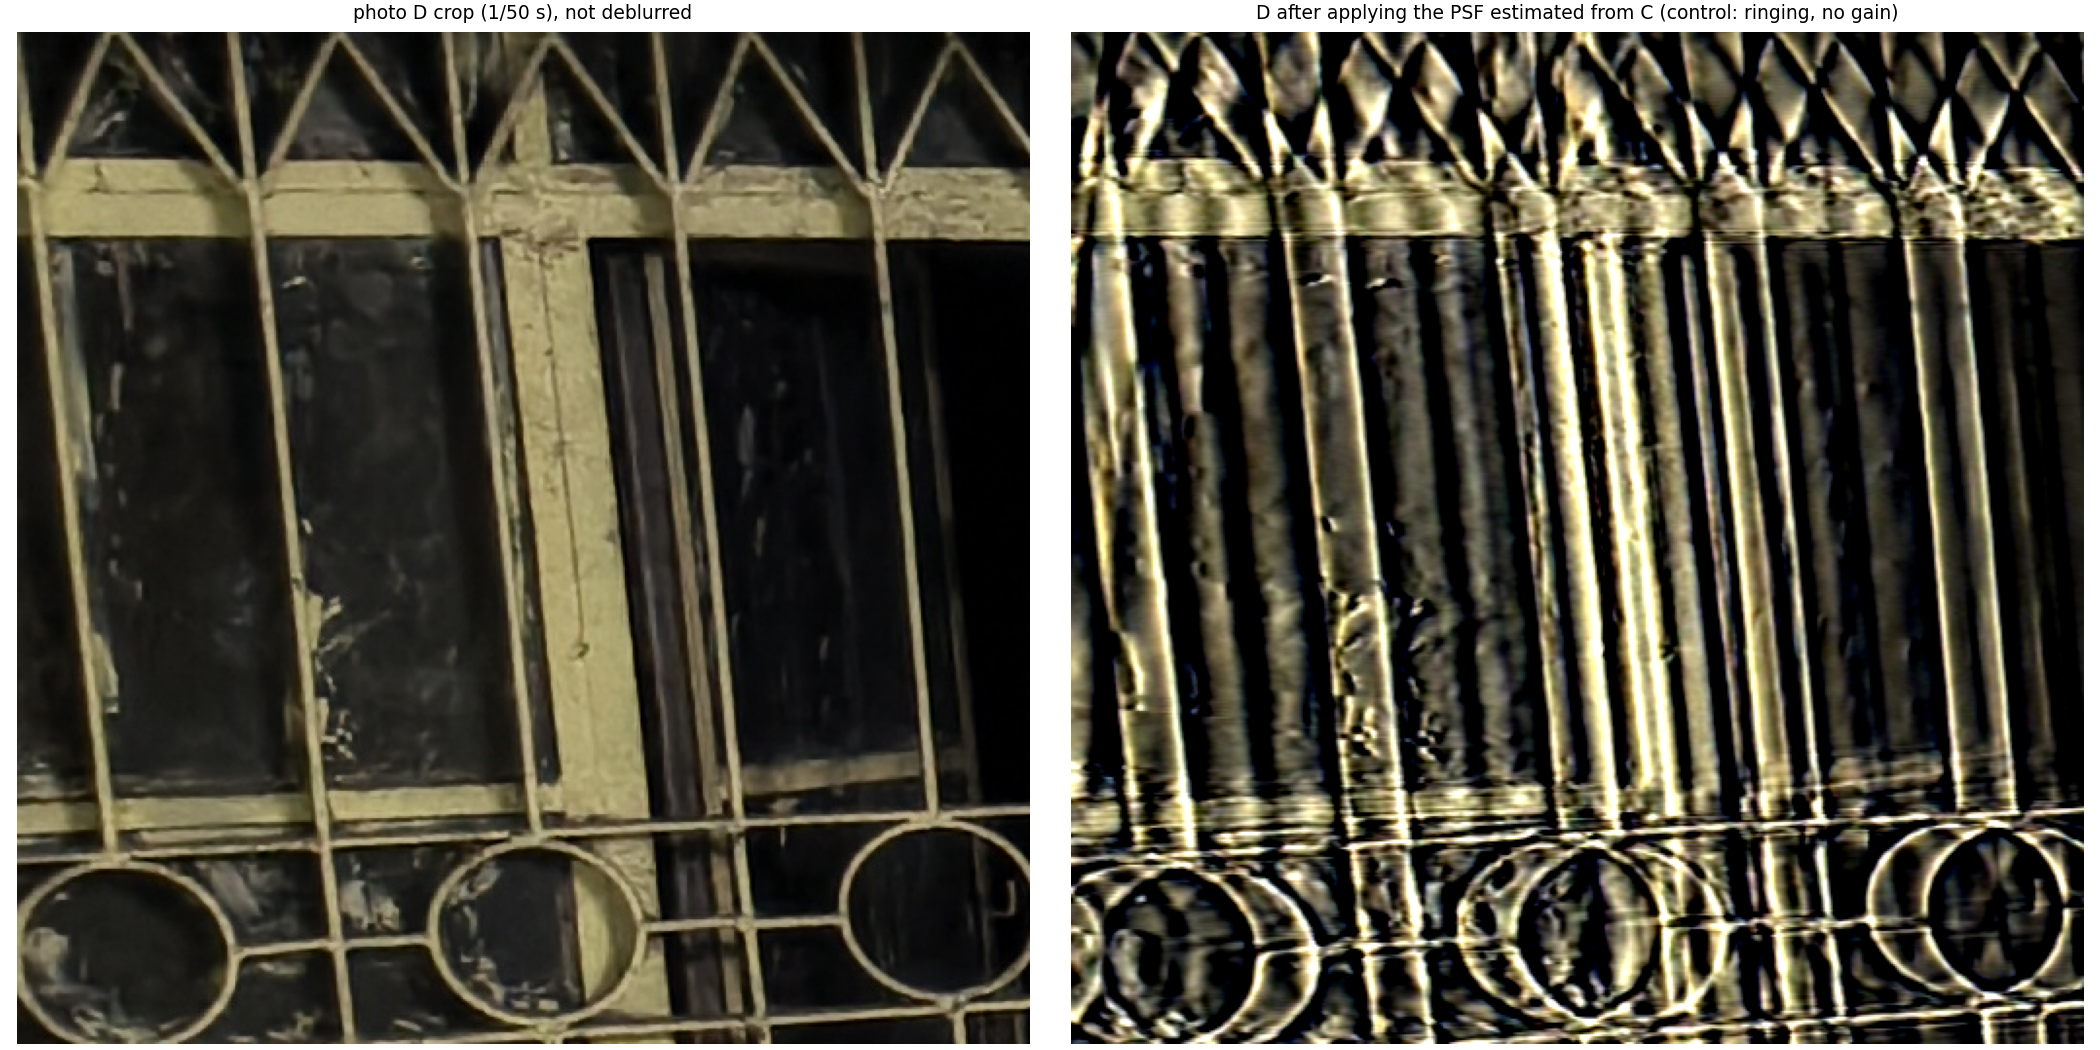
\includegraphics[width=0.85\linewidth]{q6_real_control_D}\par\vskip 3pt{\small\textbf{Figure 6.8.} Control: photograph D (sharper), left; the same Wiener deconvolution with the PSF estimated from C, right: ringing and over-sharpening only.\par}\end{figure}
\textbf{Visible artefacts and the limits of the linear, spatially invariant motion model.} (1) \textit{Ringing/overshoot} around high-contrast bars (dark and bright rims beside window bars; 19\% of the output pixels leave [0,255] at $K_{est}$ and 9\% at the adopted $K$): the PSF has zeros, the length estimate is only good to a few percent (range 32.0-34.5 px) and an error in $L$ moves the zeros away from the true ones. (2) \textit{Non-uniform blur / camera rotation:} camera shake usually contains rotation as well as translation, so blur length and direction vary over the frame (rotation about the optical axis gives arc-shaped blur growing with the distance from the centre). The single global PSF fits the window region, is too long for the floor region and has the wrong shape at the clock: the clock outline shows curved double contours and a halo (Figure 6.7, right). (3) \textit{Changing velocity:} camera shake is not constant-speed motion, the true PSF is not a box and has no clean zeros (the double ratio shows only weak, shallow undulations after the first lobe), so the box PSF reproduces the first lobe only. (4) \textit{Clipped highlights and occlusion:} saturated pixels (the bright door and the tube light) do not follow the linear model (the recorded value is min(255, convolution)), and regions where objects move across the frame are not the convolution of one sharp image; ringing appears around them. (5) \textit{Noise model:} the noise is not white (Section 5.2), so a scalar $K$ cannot be right at all frequencies.

\textbf{Reported values.} Estimated direction $\hat\theta=3.8^\circ$ (from $+x$ towards $+y$: almost horizontal), estimated length $\hat L=33.0$ px (at the native 4080x3072 resolution), scalar regularisation $K=1.41e-02$ (the noise-based $K_{est}=1.41e-03$ times 10). Automatic and adopted values of $\theta$ and $L$ coincide; only $K$ was adjusted, by inspection.

\section{7. Conclusions and limitations}
\textbf{Conclusions.} In each problem a closed-form prediction was compared with measurement, and where the two disagree the violated assumption is identified. The 8.95\% Gibbs overshoot of the ideal low-pass filter describes an edge whose neighbourhood is one-dimensional on the scale of the ripple; it does not describe small cutoffs applied to a 256-pixel square (Section 2.2). The analytic bilateral weight-ratio half-point (NCR = 0.347) and the measured edge-retention threshold are different quantities and are not expected to coincide (Section 4.3). The optimality of the Wiener filter is a statement about linear estimators under stationary second-order statistics: a locally adaptive nonlinear filter can exceed it on PSNR (Section 5.1), and the correlated, signal-dependent noise of the real photograph violates its assumptions (Section 5.2b). Several results rely on parameters tuned with the clean reference (marked oracle-tuned); they show what is attainable, not what a blind user would obtain.

\textbf{Limitations.}

\begin{itemize}\item \textbf{Real photographs.} A/B and C/D are not aligned clean/degraded pairs, so no PSNR/SSIM/MSE is computed on them. The blur of C is non-uniform: the estimated direction and length are a global effective value, the box PSF reproduces only the first lobe of the transfer function, and K for the real deblurring was chosen by inspection. \item \textbf{Resolutions.} Synthetic Q5/Q6 experiments use a 2x2 block-mean reduction of the instructor image (1536x1024, both sides \textgreater{}= 1024); Q3 uses a 3x reduction of the tunnel image; the real-photo analyses use native-resolution crops (1024x1024) and, for noise statistics, the full 4080x3072 frames. Derived images are stored separately in \texttt{data/\allowbreak{}derived/\allowbreak{}}; the four original photographs are unmodified (SHA-256 recorded). \item \textbf{Search grids.} Q5's oracle low-pass cutoff grid ends at 0.5 cycles/pixel (the sigma = 5 optimum sits at the edge); Q4's bilateral window is capped at 25x25 so the strength match cannot be reached for N \textgreater{}= 11 at sigma\_r = 2 sigma (reported in Table 4.1). \item \textbf{Timings.} Wall-clock timings depend on the hardware (Table 0.1) and are reported for orientation only. \end{itemize}
\section{8. Code and reproducibility}
Source code, experiment scripts, data-processing utilities and reproducibility instructions are available in the project repository:

\texttt{https:/\allowbreak{}/\allowbreak{}github.\allowbreak{}com/\allowbreak{}shouryasarkar713/\allowbreak{}dip-assignment-2}

The repository is private; access must be requested from the author. It contains the implementation of each question (\texttt{src/\allowbreak{}}), the input data and photographs (\texttt{data/\allowbreak{}}), the result files (\texttt{results/\allowbreak{}}), the figures (\texttt{figures/\allowbreak{}}), the tests (\texttt{tests/\allowbreak{}}) and the sources of this report (\texttt{report/\allowbreak{}}).

All random numbers come from \texttt{numpy.\allowbreak{}random.\allowbreak{}default\_\allowbreak{}rng} with fixed seeds. \texttt{python run\_\allowbreak{}all.\allowbreak{}py} regenerates the results and figures from the supplied inputs, and \texttt{python report/\allowbreak{}build\_\allowbreak{}report.\allowbreak{}py} regenerates the PDF and DOCX report from them. On a different software stack the numbers can differ at floating-point rounding level.

\end{document}